\documentclass[11pt,a4paper]{article}
\usepackage[margin=24mm,headheight=14pt]{geometry}
\usepackage[T1]{fontenc}
\usepackage[utf8]{inputenc}
\usepackage{lmodern,amssymb}
\usepackage{babel}
\babelprovide[import,main]{portuguese}
\usepackage{amsmath,amsthm,mathtools}

\PassOptionsToPackage{obeyspaces,spaces}{url}% preserva os espaços em \code{...} (identificadores Lean)
\usepackage{microtype,graphicx,xcolor,booktabs,longtable,array,float,tabularx,multicol,placeins,mathrsfs,xurl}
\usepackage{enumitem}
\usepackage{tikz}
\usetikzlibrary{arrows.meta,positioning,calc,fit}
\usepackage[round,authoryear]{natbib}
\usepackage{caption}
\captionsetup{font=small,labelfont=bf,skip=7pt}
\usepackage{fancyhdr}
\usepackage{hyperref}
\usepackage[nameinlink,noabbrev]{cleveref}
\definecolor{ink}{HTML}{172C3C}
\definecolor{accent}{HTML}{166F80}
\hypersetup{colorlinks=true,linkcolor=ink,citecolor=ink,urlcolor=accent,
 pdftitle={Biblioteca determinística de segmentos afins racionais em células diádicas: endereçamento, aproximação e refinamento certificado},
 pdfauthor={Victor Gabriel de Oliveira},
 pdfsubject={Construção racional, aproximação certificada e descrição aritmética}}
\pagestyle{fancy}
\fancyhf{}
\fancyhead[L]{\small\itshape Biblioteca determinística de segmentos afins racionais}
\fancyfoot[C]{\small\thepage}
\renewcommand{\headrulewidth}{0pt}
\setlength{\parindent}{1.25em}
\setlength{\parskip}{2pt}
\setlength{\emergencystretch}{2em}
\setlength{\textfloatsep}{15pt plus 3pt minus 3pt}
\setlength{\intextsep}{14pt plus 3pt minus 3pt}
\setlist{nosep,leftmargin=2em}
\newtheoremstyle{preciso}{8pt}{5pt}{\itshape}{}{\bfseries}{.}{.5em}{}
\theoremstyle{preciso}
\newtheorem{teorema}{Teorema}[section]
\newtheorem{lema}[teorema]{Lema}
\newtheorem{proposicao}[teorema]{Proposição}
\newtheorem{corolario}[teorema]{Corolário}
\theoremstyle{definition}
\newtheorem{definicao}[teorema]{Definição}
\newtheorem{algoritmo}[teorema]{Algoritmo}
\newtheorem{observacao}[teorema]{Observação}
\renewcommand{\proofname}{Demonstração}
\newcommand{\N}{\mathbb N}
\newcommand{\Z}{\mathbb Z}
\newcommand{\Q}{\mathbb Q}
\newcommand{\R}{\mathbb R}
\newcommand{\D}{\mathbb D}
\newcommand{\LL}{\mathcal L}
\newcommand{\Asm}{\mathcal A}
\newcommand{\FF}{\mathcal F}
\newcommand{\EE}{\mathcal E}
\newcommand{\RR}{\mathcal R}
\newcommand{\CC}{\mathcal C}
\newcommand{\heightq}{\operatorname{ht}}
\newcommand{\rank}{\operatorname{rank}}
\newcommand{\Eval}{\operatorname{Eval}}
\newcommand{\ser}{\operatorname{ser}}
\newcommand{\norm}[1]{\left\|#1\right\|_{\infty}}
\newcommand{\normK}[2]{\left\|#1\right\|_{\infty,#2}}
\newcommand{\eqn}[2]{\begin{equation}\label{eq:#1}#2\end{equation}}
\newcommand{\figura}[4]{\begin{figure}[!htbp]\centering
 \includegraphics[width=#2\linewidth]{figuras/#1.pdf}
 \caption{#3}\label{fig:#4}\end{figure}}

\newcommand{\Atoms}{\mathsf{Atom}}
\newcommand{\Cell}{\mathsf{Cell}}
\newcommand{\CK}{\mathsf C_K}
\newcommand{\Fin}{\operatorname{Fin}}
\newcommand{\FS}{\operatorname{Finset}}
\newcommand{\card}{\operatorname{card}}
\newcommand{\htq}{\operatorname{ht}}
\newcommand{\Norm}{\operatorname{Norm}}
\newcommand{\Act}{\operatorname{Active}}
\newcommand{\Sep}{\operatorname{Sep}}
\newcommand{\Cov}{\operatorname{Cover}}
\newcommand{\Match}{\operatorname{Match}}
\newcommand{\Agree}{\operatorname{Agree}}
\newcommand{\Loc}{\operatorname{LocalRep}}
\newcommand{\Str}{\operatorname{StrongRep}}
\newcommand{\Res}{\operatorname{Res}}
\newcommand{\ImageRes}{\operatorname{ResImage}}
\newcommand{\Aloc}{\mathcal A^{\mathrm{loc}}}
\newcommand{\Astr}{\mathcal A^{\mathrm{con}}}
\newcommand{\List}{\operatorname{List}}
\newcommand{\pos}{\operatorname{pos}}
\newcommand{\dec}{\operatorname{dec}}
\newcommand{\enc}{\operatorname{enc}}
\newcommand{\pred}{\operatorname{Pred}}
\newcommand{\rankq}{\operatorname{rank}}
\newcommand{\qstar}{\Q^{\times}}
\newcommand{\co}{\operatorname{coef}}
\newcommand{\cls}{\operatorname{closure}}
\newcommand{\intr}{\operatorname{interior}}
\newcommand{\ERealPos}{\overline{\R}_{\ge0}}
\newcommand{\code}[1]{\nolinkurl{#1}}
\newcommand{\crefrangeconjunction}{ a }
\newcommand{\crefpairconjunction}{ e }
\newcommand{\crefmiddleconjunction}{, }
\newcommand{\creflastconjunction}{ e }
\newcommand{\Nzero}{\mathbb{N}_0}
\newcommand{\Qstar}{\mathbb{Q}^{\!*}}
\newcommand{\Dmid}{\mathbb{D}_{\mathrm{mid}}}
\newcommand{\Aclass}{\mathcal{A}}
\newcommand{\Library}{\mathcal{L}}
\newcommand{\Intervals}{\mathcal{I}}
\newcommand{\Representations}{\mathfrak{R}}
\newcommand{\Trees}{\mathfrak{T}}
\newcommand{\Values}{\mathcal{V}}
\newcommand{\Pairs}{\mathcal{P}}
\newcommand{\height}{\operatorname{ht}}
\newcommand{\own}{\mathrm{own}}
\newcommand{\cost}{\mathcal{J}}
\newcommand{\loss}{\mathcal{E}}
\newcommand{\dd}{\,\mathrm{d}}
\newcommand{\runningtitle}{Custo, seleção exata e interpolação diádica}
\crefname{section}{seção}{seções}
\Crefname{section}{Seção}{Seções}
\crefname{subsection}{subseção}{subseções}
\Crefname{subsection}{Subseção}{Subseções}
\crefname{figure}{figura}{figuras}
\Crefname{figure}{Figura}{Figuras}
\crefname{table}{tabela}{tabelas}
\Crefname{table}{Tabela}{Tabelas}
\crefname{equation}{equação}{equações}
\Crefname{equation}{Equação}{Equações}
\crefname{appendix}{apêndice}{apêndices}
\Crefname{appendix}{Apêndice}{Apêndices}
\crefname{theorem}{teorema}{teoremas}
\crefname{lemma}{lema}{lemas}
\crefname{proposition}{proposição}{proposições}
\crefname{corollary}{corolário}{corolários}
\crefname{definition}{definição}{definições}
\crefname{algorithm}{algoritmo}{algoritmos}
\crefname{remark}{observação}{observações}
\DeclareMathOperator*{\argmin}{arg\,min}
\theoremstyle{preciso}
\newtheorem{theorem}[teorema]{Teorema}
\theoremstyle{preciso}
\newtheorem{lemma}[teorema]{Lema}
\theoremstyle{preciso}
\newtheorem{proposition}[teorema]{Proposição}
\theoremstyle{preciso}
\newtheorem{corollary}[teorema]{Corolário}
\theoremstyle{definition}
\newtheorem{definition}[teorema]{Definição}
\theoremstyle{preciso}
\newtheorem{algorithm}[teorema]{Algoritmo}
\theoremstyle{definition}
\newtheorem{remark}[teorema]{Observação}
% Ambientes sem numeração (acréscimos editoriais): não alteram contadores nem o mapa de 151 ambientes.
\theoremstyle{preciso}
\newtheorem*{proposicaoSN}{Proposição (ponte entre as Partes~I e~III)}
\theoremstyle{definition}
\newtheorem*{observacaoSN}{Observação}

\renewcommand{\partname}{Parte}
\renewcommand{\contentsname}{Sumário}
\renewcommand{\refname}{Referências}
\renewcommand{\thesection}{\Roman{part}.\arabic{section}}
\renewcommand{\thefigure}{\Roman{part}.\arabic{figure}}
\renewcommand{\thetable}{\Roman{part}.\arabic{table}}
\renewcommand{\theequation}{\Roman{part}.\arabic{equation}}
\renewcommand{\theHsection}{\thesection}
\renewcommand{\theHfigure}{\arabic{part}.\arabic{figure}}
\renewcommand{\theHtable}{\arabic{part}.\arabic{table}}
\renewcommand{\theHequation}{\arabic{part}.\arabic{equation}}
\newcommand{\volumeparte}[1]{\clearpage\part{#1}\setcounter{section}{0}\setcounter{figure}{0}\setcounter{table}{0}\setcounter{equation}{0}\renewcommand{\thesection}{\Roman{part}.\arabic{section}}}
\makeatletter
\renewcommand*{\l@section}{\@dottedtocline{1}{1.5em}{4em}}
\renewcommand*{\l@subsection}{\@dottedtocline{2}{4em}{5em}}
\renewcommand*{\l@subsubsection}{\@dottedtocline{3}{8em}{6em}}
\makeatother
\fancyhead[L]{\small\itshape Biblioteca determinística: volume unificado}
\hypersetup{pdftitle={Biblioteca determinística: volume unificado e correspondência Lean 4},pdfauthor={Victor Gabriel de Oliveira}}
\title{\bfseries Biblioteca determinística de segmentos afins racionais\\[8pt]\Large Construção, seleção, aproximação e normalização\\[8pt]\large Volume unificado com correspondência Lean 4}
\author{Victor Gabriel de Oliveira}
\date{Edição consolidada de 13 de novembro de 2026}
\begin{document}
\maketitle
\begin{abstract}
Este volume reúne a construção da biblioteca racional em células diádicas, a normalização das montagens, os custos aritméticos e a seleção exata, a teoria direta--inversa e os complementos do manuscrito de 77 páginas. Os enunciados e as demonstrações disponíveis são preservados em cinco partes. A correspondência final relaciona os 151 ambientes da edição atual aos fontes Lean existentes e aos 108 ambientes do manuscrito original. As diferenças semânticas e os resultados ainda sem formalização localizada permanecem identificados.
\end{abstract}
\section*{Convenções desta edição}
A numeração tem a forma parte.seção.resultado. As remissões numéricas textuais herdadas dos artigos usam a numeração local da própria parte, salvo indicação explícita de outro artigo. A Parte I corresponde ao Artigo 1; a Parte II contém a normalização auxiliar; as Partes III e IV correspondem aos Artigos 2 e 3; a Parte V conserva os complementos das seções 6 e 21 originais. A correspondência documental reúne os destinos do original sem duplicar seu bloco de custo aritmético.

Os fontes Lean recebidos permanecem inalterados; as novas provas ficam nas bibliotecas \texttt{Pendencias} e \texttt{PendenciasParte1}. Em 13 de novembro de 2026, os três ambientes foram recompilados e as auditorias dessas bibliotecas encontraram apenas \texttt{propext}, \texttt{Classical.choice} e \texttt{Quot.sound}. Correspondência herdada e prova compilada permanecem categorias distintas. A pasta \texttt{Fase3} pertence à base do Artigo 1. Quatro dos 42 casos do dossiê original permanecem sem fechamento completo, com motivos registrados no pacote; não se afirma formalização integral.
\tableofcontents

% I | fonte original: artigos/artigo_1/artigo.tex
\volumeparte{Biblioteca, endereçamento e refinamento}
% Reconstruído de artigos/artigo_1/artigo.tex
\renewcommand{\eqn}[2]{\begin{equation}\label{artigo_1:eq:#1}#2\end{equation}}



% INICIO artigos/artigo_1/secoes/00_resumos.tex
\begin{abstract}
Construímos uma biblioteca enumerável, sem repetições, de segmentos afins de inclinação racional não nula ancorados em células diádicas. Cada endereço recupera exatamente a célula e a função afim. Montagens contínuas finitas são densas em $C(K)$ e admitem representação exata por redes ReLU rasas racionais com quebras diádicas. Para funções $C^2$, a racionalização preserva a constante $1/8$ do erro interpolatório uniforme. O refinamento adaptativo combina majorantes intervalares racionais da segunda derivada e racionalização nodal, com correção, término e tamanho controlados sob as hipóteses explicitadas. A contagem por altura, os custos de codificação, a entropia e a seleção em catálogos finitos são desenvolvidos no segundo artigo da série.

\smallskip\noindent\textbf{Palavras-chave:} aproximação linear por partes; células diádicas; altura aritmética; endereçamento; refinamento certificado; redes ReLU.
\end{abstract}

\begingroup\small
\begin{center}\textbf{Abstract}\end{center}
\noindent We construct a repetition-free enumerable library of affine segments with nonzero rational slopes anchored on dyadic cells. Each address recovers the cell and the affine function exactly. Finite continuous assemblies are dense in $C(K)$ and admit exact representations as rational shallow ReLU networks with dyadic breakpoints. For $C^2$ functions, rationalization preserves the constant $1/8$ in uniform interpolation error. Adaptive refinement combines rational interval bounds for the second derivative and nodal rationalization, with correctness, termination and size bounds under the stated hypotheses. Height counting, coding costs, entropy and selection in finite catalogs are developed in the second article of the series.

\smallskip\noindent\textbf{Keywords:} piecewise-linear approximation; dyadic cells; arithmetic height; addressing; certified refinement; ReLU networks.
\endgroup
% FIM artigos/artigo_1/secoes/00_resumos.tex
% INICIO artigos/artigo_1/secoes/01_introducao.tex
\section{Introdução}
Representar uma curva por segmentos afins envolve erro, número de peças e tamanho aritmético dos parâmetros. Este artigo constrói uma biblioteca de segmentos racionais ancorados em células diádicas. Cada átomo possui endereço único e uma interface global que recupera seu suporte.

A aproximação linear por partes, a escolha de nós e a aproximação não linear têm tratamento clássico em \citet{artigo_1-deboor1973,artigo_1-burchard1974,artigo_1-deboor2001,artigo_1-powell1981,artigo_1-schumaker2007,artigo_1-devore1998}. A representação por hinges e sua relação com redes ReLU são desenvolvidas em \citet{artigo_1-yarotsky2017,artigo_1-devore2021,artigo_1-daubechies2022}; a aproximação com pesos codificáveis, em \citet{artigo_1-petersen2018,artigo_1-elbrachter2021,artigo_1-bolcskei2019,artigo_1-guhring2021}. Aqui, esses resultados se integram a uma parametrização racional com recuperação exata da célula.

A construção usa a altura elementar dos racionais \citep{artigo_1-bombieri2006} e distingue a enumeração por altura da ordem de Calkin--Wilf \citep{artigo_1-calkin2000}, relacionada à sequência de Stern \citep{artigo_1-stern1858,artigo_1-northshield2010}. O refinamento combina aproximação em árvores \citep{artigo_1-cohen2001,artigo_1-binev2004,artigo_1-kessebohmer2025} com aritmética intervalar \citep{artigo_1-moore2009,artigo_1-silva2025}.

O modelo fixa inclinações não nulas para tornar o suporte recuperável pela imagem do segmento. A certificação adaptativa requer majorantes validados da segunda derivada; testes em pontos isolados não substituem esse contrato. A quantização diádica é distinguida da escolha de nós livres.

A exposição progride da indexação à biblioteca, das montagens às garantias de aproximação uniforme e destas ao refinamento certificado. A contagem de átomos, os limites minimax do endereçamento, os formatos de codificação, a entropia e a seleção em catálogos finitos ficam no segundo artigo da série. Os resultados clássicos sobre árvores, nós livres e Besov e o lema auxiliar de Runge permanecem integralmente no complemento do manuscrito original, com a numeração de origem preservada.
% FIM artigos/artigo_1/secoes/01_introducao.tex
% INICIO artigos/artigo_1/secoes/02_indexacao.tex
\section{Ferramentas de indexação}
Escreva $\N_0=\{0,1,2,\ldots\}$ e $T_m=m(m+1)/2$.

\subsection{Pareamento de Cantor}
Para $u,v\in\N_0$, defina
\eqn{01}{\pi(u,v)=T_{u+v}+v=\frac{(u+v)(u+v+1)}2+v.}
% MAPA artigo_1:2.1 | fonte artigos/artigo_1/secoes/02_indexacao.tex:7
\begin{lema}[pareamento e cota]\label{map:artigo_1:2.1}
$\pi:\N_0^2\to\N_0$ é bijetiva. Para $n\in\N_0$, sua inversa é
\eqn{02}{w=\left\lfloor\frac{\sqrt{8n+1}-1}{2}\right\rfloor,\qquad v=n-T_w,\qquad u=w-v.}
Além disso, $\pi(u,v)\le(u+v+1)^2$.
\end{lema}
\begin{proof}
Se $m=u+v$, então $T_m\le\pi(u,v)=T_m+v<T_{m+1}$, pois $0\le v\le m$. Assim, cada imagem pertence a um único bloco diagonal $[T_m,T_{m+1})$. Dado $n$, a expressão para $w$ em \eqref{artigo_1:eq:02} é precisamente o único inteiro com $T_w\le n<T_{w+1}$. Logo $0\le v=n-T_w\le w$, $u=w-v\ge0$ e $\pi(u,v)=n$, provando sobrejetividade. O bloco determina $w=u+v$ e, dentro dele, $v=n-T_w$; portanto o par é único. Por fim, com $x=u+v+1$, tem-se $T_{u+v}\le x^2/2$ e $v\le x^2/2$, donde $\pi(u,v)\le x^2$.
\end{proof}

\subsection{Inteiros e racionais por altura}
Defina $Z:\N_0\to\Z$ por
\eqn{03}{Z(t)=\begin{cases}t/2,&t\text{ par},\\-(t+1)/2,&t\text{ ímpar}.\end{cases}}
% MAPA artigo_1:2.2 | fonte artigos/artigo_1/secoes/02_indexacao.tex:19
\begin{lema}\label{map:artigo_1:2.2}
$Z$ é bijetiva, com $Z^{-1}(m)=2m$ para $m\ge0$ e $Z^{-1}(m)=-2m-1$ para $m<0$. Em particular, $Z^{-1}(m)\le2|m|+1$.
\end{lema}
\begin{proof}
Os índices pares percorrem $\N_0$ exatamente uma vez; os ímpares percorrem $\Z\setminus\N_0$ exatamente uma vez. As duas imagens são disjuntas e as fórmulas inversas resultam por resolução direta de \eqref{artigo_1:eq:03}.
\end{proof}

Todo $r\in\Q$ tem uma representação reduzida única $p/q$, com $p\in\Z$, $q\in\N$ e $\gcd(|p|,q)=1$. Adote a altura multiplicativa elementar
\eqn{04}{\heightq(p/q)=\max\{|p|,q\}.}
Ordene os pares reduzidos primeiro por altura, depois por $q$ e finalmente por $p$. Essa leitura define bijeções
\eqn{05}{Q:\N_0\to\Q,\qquad Q^*:\N_0\to\Q^*,}
na segunda das quais se omite $0/1$.

% MAPA artigo_1:2.3 | fonte artigos/artigo_1/secoes/02_indexacao.tex:32
\begin{lema}[contagem por altura]\label{map:artigo_1:2.3}
Seja $\Q_H=\{r\in\Q:\heightq(r)\le H\}$. Então
\eqn{06}{|\Q_H|\le3H^2\qquad\text{para todo }H\ge1,}
e existem $H_0$ e $c_1>0$ universais tais que
\eqn{07}{|\Q_H|\ge c_1H^2\qquad\text{para todo }H\ge H_0.}
Pode-se tomar $c_1=1/4$.
\end{lema}
\begin{proof}
A forma reduzida com denominador positivo é única: de $p/q=p'/q'$ e das duas coprimalidades segue $q\mid q'$ e $q'\mid q$, logo $q=q'$ e $p=p'$. Cada $r\in\Q_H$ corresponde então a um único par $(p,q)$ com $|p|\le H$ e $1\le q\le H$; há no máximo $(2H+1)H\le3H^2$ tais pares, o que prova \eqref{artigo_1:eq:06}.

Para \eqref{artigo_1:eq:07}, observe que $\Q_H$ contém todas as frações $p/q$ com $1\le q\le H$, $1\le p\le q$ e $\gcd(p,q)=1$, cuja quantidade é $\Phi(H)=\sum_{q\le H}\varphi(q)$. Pelo teorema clássico de Mertens sobre a soma de Euler \citep[Teorema 330]{artigo_1-hardy2008},
\[
\Phi(H)=\frac3{\pi^2}H^2+O(H\log H),
\]
e $3/\pi^2>0{,}30$. Logo $\Phi(H)\ge H^2/4$ para todo $H$ suficientemente grande.
\end{proof}

% MAPA artigo_1:2.4 | fonte artigos/artigo_1/secoes/02_indexacao.tex:49
\begin{lema}[posto por altura]\label{map:artigo_1:2.4}
As aplicações em \eqref{artigo_1:eq:05} são bijetivas. Se $\heightq(p/q)\le H$, então o posto de $p/q$ em qualquer uma delas é estritamente menor que $3H^2$.
\end{lema}
\begin{proof}
A ordenação esgota cada casca finita de altura antes de passar à seguinte; portanto lista todo racional uma única vez, o que dá a bijetividade. Todo elemento que precede $p/q$ pertence a $\Q_H$, e o lema~2.3 limita essa cardinalidade por $3H^2$. A remoção de $0/1$ em $Q^*$ só diminui a contagem.
\end{proof}

\subsection{Bijetividade e crescimento do índice}
A ordem de Calkin--Wilf fornece uma comparação entre bijetividade e crescimento do endereço. Seja $(S_n)_{n\ge0}$ a sequência diatômica de Stern,
\eqn{08}{S_0=0,\qquad S_1=1,\qquad S_{2n}=S_n,\qquad S_{2n+1}=S_n+S_{n+1},}
e $CW(n)=S_n/S_{n+1}$, $n\ge1$, que enumera $\Q_{>0}$ sem repetições.
% MAPA artigo_1:2.5 | fonte artigos/artigo_1/secoes/02_indexacao.tex:60
\begin{lema}\label{map:artigo_1:2.5}
Para todo $q\ge1$, $CW(2^{q-1})=1/q$.
\end{lema}
\begin{proof}
Da recorrência par, $S_{2^m}=S_1=1$. Também $S_{2^m+1}=m+1$: o caso $m=0$ é $S_2=1$ e
\[
S_{2^{m+1}+1}=S_{2(2^m)+1}=S_{2^m}+S_{2^m+1}=1+(m+1).
\]
Tomando $m=q-1$, resulta $CW(2^{q-1})=1/q$.
\end{proof}

O racional $1/q$ tem altura $q$, mas índice $2^{q-1}$; a escrita binária do índice exige $q$ bits, contra os $O(\log q)$ do lema~2.4. A ordenação por altura controla o endereço em função de $\heightq(r)$. A \cref{artigo_2:sec:complexity} determina o comprimento mínimo no pior caso por contagem e constrói uma enumeração que o realiza.
\begin{figure}[!htbp]\centering
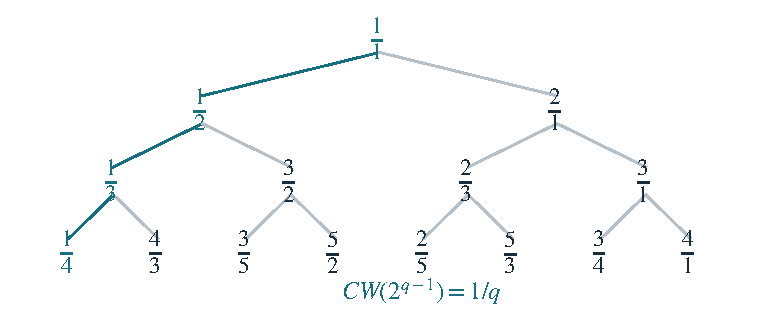
\includegraphics[width=.94\linewidth]{figuras/artigo_1/01_calkin_wilf.pdf}
\caption{Primeiros níveis da árvore de Calkin--Wilf. O ramo esquerdo contém $1/q$ no índice $2^{q-1}$; a ordenação por altura fornece índices polinomiais na altura.}\label{artigo_1:fig:cw}\end{figure}
% FIM artigos/artigo_1/secoes/02_indexacao.tex
% INICIO artigos/artigo_1/secoes/03_biblioteca.tex
\section{Células diádicas e operador gerador}
\subsection{Células, posse e centros}
Para $k\in\N_0$ e $m\in\Z$, sejam
\eqn{09}{J_{k,m}=[m2^{-k},(m+1)2^{-k}],\qquad J_{k,m}^{\rm own}=[m2^{-k},(m+1)2^{-k}),}
e
\eqn{10}{x_0(k,m)=\left(m+\frac12\right)2^{-k}=\frac{2m+1}{2^{k+1}}.}
A célula fechada sustenta o segmento; a versão semiaberta atribui cada fronteira a um único proprietário. Escreva
\[
\D=\{j2^{-K}:j\in\Z,\ K\in\N_0\},\qquad \D_{\rm mid}=\D\setminus\Z.
\]
% MAPA artigo_1:3.1 | fonte artigos/artigo_1/secoes/03_biblioteca.tex:11
\begin{lema}[estrutura diádica]\label{map:artigo_1:3.1}
Para cada $k$, as células $J_{k,m}^{\rm own}$ particionam $\R$ e
\eqn{11}{J_{k,m}=J_{k+1,2m}\cup J_{k+1,2m+1},\qquad |J_{k,m}|=2^{-k}.}
O mapa $(k,m)\mapsto x_0(k,m)$ é uma bijeção de $\N_0\times\Z$ sobre $\D_{\rm mid}$, que é denso em $\R$.
\end{lema}
\begin{proof}
Para $x\in\R$, o único índice de posse na escala $k$ é $m=\lfloor2^kx\rfloor$; isso prova a partição. A identidade de refinamento decorre de cindir $[2m2^{-(k+1)},(2m+2)2^{-(k+1)}]$ em seu ponto médio.

Pela \eqref{artigo_1:eq:10}, o centro tem numerador ímpar e denominador reduzido $2^{k+1}\ge2$, logo pertence a $\D_{\rm mid}$. Reciprocamente, cada $x\in\D_{\rm mid}$ possui forma reduzida única $j/2^K$, com $K\ge1$ e $j$ ímpar; tomando $k=K-1$ e $m=(j-1)/2$, obtém-se $x=x_0(k,m)$. A mesma unicidade prova a injetividade. Por fim, os centros de escala $k$ estão espaçados por $2^{-k}$; escolhendo o mais próximo de um real dado, a distância tende a zero com $k$, o que prova a densidade.
\end{proof}
\begin{figure}[!htbp]\centering
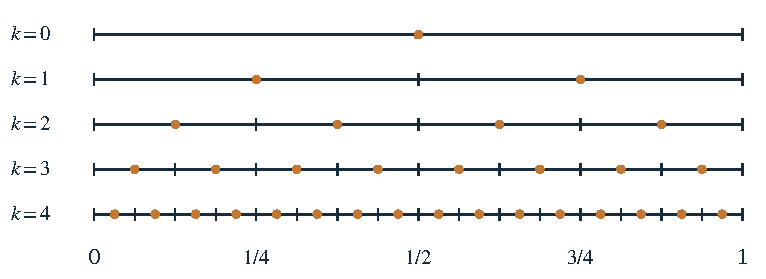
\includegraphics[width=.92\linewidth]{figuras/artigo_1/02_celulas.pdf}
\caption{Células diádicas, centros e posse das fronteiras. Cada célula se divide em dois filhos; os centros determinam a célula de origem.}\label{artigo_1:fig:celulas}\end{figure}

\subsection{Retas ancoradas e descompactação}
Dados $x_0,y_0\in\R$ e $s\ne0$, a reta ancorada é
\eqn{12}{\ell(x)=y_0+s(x-x_0)=a+bx,\qquad b=s,\quad a=y_0-sx_0.}
Para $n\in\N_0$, aplique sucessivamente a inversa do pareamento:
\eqn{13}{(u,v)=\pi^{-1}(n),\qquad(k,\mu)=\pi^{-1}(u),\qquad(r,t)=\pi^{-1}(v).}
% MAPA artigo_1:3.2 | fonte artigos/artigo_1/secoes/03_biblioteca.tex:28
\begin{lema}\label{map:artigo_1:3.2}
O mapa $n\mapsto(k,\mu,r,t)$ de \eqref{artigo_1:eq:13} é uma bijeção de $\N_0$ sobre $\N_0^4$.
\end{lema}
\begin{proof}
Sua inversa explícita é
\[
(k,\mu,r,t)\longmapsto\pi\bigl(\pi(k,\mu),\pi(r,t)\bigr),
\]
uma composição de bijeções pelo lema~2.1.
\end{proof}
Defina
\eqn{14}{m=Z(\mu),\quad x_{0,n}=x_0(k,m),\quad y_{0,n}=Q(r),\quad s_n=Q^*(t),}
e converta para a forma global por
\eqn{15}{b_n=s_n,\qquad a_n=y_{0,n}-s_nx_{0,n}.}
Se $x_L=m2^{-k}$ e $x_R=(m+1)2^{-k}$, ponha
\eqn{16}{c_n=\min\{\ell_n(x_L),\ell_n(x_R)\},\qquad d_n=\max\{\ell_n(x_L),\ell_n(x_R)\}.}
% MAPA artigo_1:3.3 | fonte artigos/artigo_1/secoes/03_biblioteca.tex:44
\begin{definicao}[gerador e biblioteca]\label{map:artigo_1:3.3}
Se $\mathcal I$ é o conjunto dos intervalos fechados não degenerados de $\R$, defina
\eqn{17}{\Gamma:\N_0\to\R\times(\R\setminus\{0\})\times\mathcal I,\qquad
\Gamma(n)=(a_n,b_n,[c_n,d_n]).}
A biblioteca é $\LL=\Gamma(\N_0)$. O átomo de endereço $n$ é a restrição de $\ell_n$ à célula $J_{k(n),m(n)}$.
\end{definicao}
Como $s_n\ne0$ e $x_L\ne x_R$, o intervalo em \eqref{artigo_1:eq:16} é não degenerado. A inclinação não nula torna a interface invertível no eixo espacial: uma peça constante teria imagem pontual e perderia a informação da célula. Para $\Gamma(n)=(a_n,b_n,[c_n,d_n])$, a pré-imagem espacial é
\eqn{18}{I_n^x=\left[
\min\left\{\frac{c_n-a_n}{b_n},\frac{d_n-a_n}{b_n}\right\},
\max\left\{\frac{c_n-a_n}{b_n},\frac{d_n-a_n}{b_n}\right\}\right].}

\subsection{Recuperação da célula e endereço canônico}
% MAPA artigo_1:3.4 | fonte artigos/artigo_1/secoes/03_biblioteca.tex:56
\begin{lema}[validade espacial exata]\label{map:artigo_1:3.4}
Para todo $n\in\N_0$, o intervalo $I_n^x$ definido em \eqref{artigo_1:eq:18} satisfaz
\[
I_n^x=J_{k(n),m(n)}.
\]
\end{lema}
\begin{proof}
Como $b_n\ne0$, $\ell_n$ é uma bijeção afim estritamente monótona. Sua restrição a $[x_L,x_R]$ tem imagem $[c_n,d_n]$ por \eqref{artigo_1:eq:16}; logo $\ell_n^{-1}([c_n,d_n])=[x_L,x_R]$. Os dois quocientes em \eqref{artigo_1:eq:18} são precisamente $\ell_n^{-1}(c_n)$ e $\ell_n^{-1}(d_n)$, possivelmente em ordem invertida quando $b_n<0$.
\end{proof}
% MAPA artigo_1:3.5 | fonte artigos/artigo_1/secoes/03_biblioteca.tex:65
\begin{teorema}[unicidade do endereço]\label{map:artigo_1:3.5}
$\Gamma$ é injetiva. Portanto, é uma bijeção de $\N_0$ sobre $\LL$ e cada átomo tem um único endereço.
\end{teorema}
\begin{proof}
Suponha $\Gamma(n)=\Gamma(n')=(a,b,[c,d])$. Pelo lema~3.4, a tripla recupera a célula comum $J=[x_L,x_R]$. Seu comprimento determina unicamente $k=-\log_2|J|$, e $m=2^kx_L$. Assim, também se recupera $x_0=(m+1/2)2^{-k}$. A inclinação local é $s=b$ e o valor ancorado é $y_0=a+bx_0$.

Pelas bijeções dos lemas~2.2, 2.4 e 3.1, os dados $(x_0,y_0,s)$ determinam unicamente $(k,\mu,r,t)$. O lema~3.2 determina então um único $n$. Logo $n=n'$.
\end{proof}
Em uma fronteira, duas células fechadas podem estar ativas. A célula semiaberta escolhe uma proprietária; em uma montagem contínua, as duas peças têm o mesmo valor no nó.
% MAPA artigo_1:3.6 | fonte artigos/artigo_1/secoes/03_biblioteca.tex:74
\begin{teorema}[dicionário de jatos racionais]\label{map:artigo_1:3.6}
O mapa
\eqn{19}{n\longmapsto(x_{0,n},y_{0,n},s_n)}
é uma bijeção de $\N_0$ sobre $\D_{\rm mid}\times\Q\times\Q^*$. Sua imagem é densa em $\R^3$.
\end{teorema}
\begin{proof}
A bijetividade resulta da composição das bijeções em \eqref{artigo_1:eq:13}--\eqref{artigo_1:eq:14}. A densidade decorre da densidade de $\D_{\rm mid}$, de $\Q$ e de $\Q^*$ em $\R$, aplicada coordenada a coordenada na norma do máximo.
\end{proof}
O dicionário \eqref{artigo_1:eq:19} parametriza todos os 1-jatos com centro diádico não inteiro, valor racional e derivada racional não nula. Montagens contínuas ligam esses dados locais por valores de fronteira compartilhados.

\subsection{Calibre dos parâmetros}
Para um átomo com dados $(k,m,y_0,s)$, usamos o mesmo calibre aritmético do segundo artigo:
\eqn{46}{H=\max\{2,k+1,|m|+1,\heightq(y_0),\heightq(s)\}.}
A definição fixa o significado da hipótese de altura na proposição~4.4; as contagens sob esse calibre são tratadas no segundo artigo.
% FIM artigos/artigo_1/secoes/03_biblioteca.tex
% INICIO artigos/artigo_1/secoes/04_montagens.tex
\section{Montagens e densidade em espaços de funções contínuas}
% MAPA artigo_1:4.1 | fonte artigos/artigo_1/secoes/04_montagens.tex:2
\begin{definicao}[montagem contínua]\label{map:artigo_1:4.1}
Se $K=[\alpha,\beta]$ é um intervalo compacto não degenerado, $\Asm(K)$ é o conjunto das funções $g\in C(K)$ para as quais existe uma coleção finita $\Lambda$ de células diádicas, com interiores disjuntos e união contendo $K$, e endereços $n(J)$, $J\in\Lambda$, tais que
\eqn{20}{g|_{J\cap K}=\ell_{n(J)}|_{J\cap K},}
com valores coincidentes nas fronteiras compartilhadas.
\end{definicao}
Para $f\in C(K)$, denote o módulo de continuidade por
\eqn{21}{\omega(f;\delta)=\sup\{|f(x)-f(y)|:x,y\in K,\ |x-y|\le\delta\}.}
O resultado seguinte impõe simultaneamente nós diádicos, valores racionais e inclinações não nulas. A figura~\ref{artigo_1:fig:montagem} mostra a ligação das peças por nós comuns.
\begin{figure}[!htbp]\centering
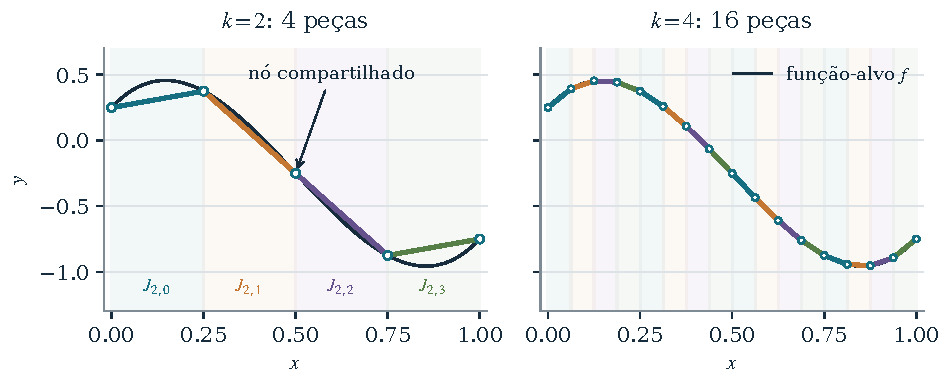
\includegraphics[width=1\linewidth]{figuras/artigo_1/03_montagem_continua.pdf}
\caption{Montagem contínua de átomos. À esquerda, cada cor identifica uma célula e seu segmento; peças consecutivas compartilham o mesmo valor no nó. À direita, o refinamento substitui células por filhos e aproxima a função-alvo com mais peças conectadas.}\label{artigo_1:fig:montagem}\end{figure}

% MAPA artigo_1:4.2 | fonte artigos/artigo_1/secoes/04_montagens.tex:12
\begin{teorema}[densidade das montagens]\label{map:artigo_1:4.2}
Para todo $f\in C[\alpha,\beta]$ e todo $\varepsilon>0$, existe $g\in\Asm([\alpha,\beta])$ tal que
\[
\normK{f-g}{[\alpha,\beta]}<\varepsilon.
\]
Todas as peças de $g$ pertencem a $\LL$ e têm inclinação não nula.
\end{teorema}
\begin{proof}
Estenda $f$ por constantes: $F(x)=f(\alpha)$ para $x<\alpha$, $F=f$ em $[\alpha,\beta]$ e $F(x)=f(\beta)$ para $x>\beta$. A extensão é uniformemente contínua. Escolha $k$ de modo que, com $h=2^{-k}$,
\eqn{22}{\omega(F;h)<\varepsilon/2.}
Tome os nós $t_j=jh$ desde $j_{\min}=\lfloor\alpha/h\rfloor$ até $j_{\max}=\lceil\beta/h\rceil$. Para cada $j$, escolha racional $v_j$ com $|v_j-F(t_j)|<\varepsilon/2$ e, sequencialmente, imponha $v_{j+1}\ne v_j$. Isso é possível porque cada intervalo aberto de escolha contém infinitos racionais e apenas um valor é proibido em cada passo.

Seja $g$ o interpolante linear dos pares $(t_j,v_j)$. Em $J_{k,j}$, sua inclinação é $(v_{j+1}-v_j)/h\in\Q^*$ e seu valor no centro é $(v_j+v_{j+1})/2\in\Q$. Pelo teorema~3.6, a peça é o único átomo com esses parâmetros. Os valores nodais compartilhados tornam $g$ contínua.

Se $P_kF$ é o interpolante dos valores exatos, então, para $x=(1-\theta)t_j+\theta t_{j+1}$,
\[
|F(x)-P_kF(x)|\le(1-\theta)|F(x)-F(t_j)|+\theta|F(x)-F(t_{j+1})|
\le\omega(F;h)<\varepsilon/2.
\]
Além disso, $P_kF-g$ é linear em cada célula e seus valores nodais têm módulo menor que $\varepsilon/2$, logo $\norm{P_kF-g}<\varepsilon/2$. A desigualdade triangular conclui.
\end{proof}
O número de células dessa cobertura uniforme é
\eqn{23}{N_k=\lceil\beta2^k\rceil-\lfloor\alpha2^k\rfloor=(\beta-\alpha)2^k+O(1).}

\subsection{Equivalência exata com redes ReLU racionais}
Escreva $\rho(z)=z_+=\max\{0,z\}$. A identidade em hinges abaixo conserva os nós diádicos, os parâmetros racionais e as inclinações não nulas da montagem.
% MAPA artigo_1:4.3 | fonte artigos/artigo_1/secoes/04_montagens.tex:38
\begin{teorema}[equivalência montagem--ReLU racional]\label{map:artigo_1:4.3}
Seja $g\in\Asm(K)$ dada por $N$ folhas consecutivas, com nós $t_0<t_1<\cdots<t_N$ e inclinação racional não nula $s_j$ em $[t_j,t_{j+1}]\cap K$, $0\le j<N$. Como $t_0$ pode estar fora de $K$, $g(t_0)$ denota o valor em $t_0$ da primeira peça $\ell_{n(J_0)}$, $J_0=[t_0,t_1]$, que coincide com $g(t_0)$ quando $t_0\in K$. Então, em $K$,
\eqn{24}{g(x)=g(t_0)+s_0(x-t_0)+\sum_{j=1}^{N-1}(s_j-s_{j-1})\rho(x-t_j).}
Depois de expandido o primeiro termo afim, todos os coeficientes são racionais, todos os pontos de quebra internos são diádicos e \eqref{artigo_1:eq:24} é uma rede ReLU rasa normalizada com $N-1$ unidades hinge e um termo afim de saída. Unidades cujo peso de saída é zero podem ser removidas.

Reciprocamente, seja
\eqn{25}{R(x)=c+qx+\sum_{j=1}^Ma_j\rho(x-\tau_j),\qquad c,q,a_j\in\Q,\quad\tau_j\in\D,}
com nós distintos. Suponha que $K$ admita uma cobertura por células diádicas compatível com os $\tau_j$, que os valores nodais sejam racionais e que cada inclinação local
\eqn{26}{q+\sum_{\tau_j<x}a_j}
seja não nula. Então $R|_K\in\Asm(K)$. Uma malha diádica uniforme que refine todos os $\tau_j$ fornece essa montagem explicitamente.
\end{teorema}
\begin{proof}
Na primeira folha, o lado direito de \eqref{artigo_1:eq:24} tem valor $g(t_0)$ em $t_0$ e inclinação $s_0$. Ao atravessar $t_j$, a derivada ganha exatamente $s_j-s_{j-1}$; por indução, sua inclinação na folha $j$ é $s_j$. Como ambos os lados são contínuos e coincidem no primeiro nó, coincidem em todo $K$. Cada $s_j$ é racional. Os nós internos são fronteiras de células diádicas, e o intercepto do primeiro átomo é racional por \eqref{artigo_1:eq:15}; logo a forma expandida tem somente parâmetros racionais.

Para a recíproca, refine uma grade diádica até que cada $\tau_j$ seja uma fronteira. Em qualquer célula aberta da grade, \eqref{artigo_1:eq:25} é afim, com inclinação \eqref{artigo_1:eq:26}. O valor no centro da célula é racional, pois o centro, os nós e todos os coeficientes são racionais. A hipótese de inclinação não nula permite aplicar o teorema~3.6, que fornece um único átomo da biblioteca nessa célula. A continuidade de $R$ faz os valores coincidirem nas fronteiras. A união das peças é, portanto, uma montagem no sentido da definição~4.1.
\end{proof}
A forma normalizada \eqref{artigo_1:eq:25} já implica valores nodais racionais. Se a arquitetura não oferecer conexão afim direta, $x=\rho(x)-\rho(-x)$ realiza o termo linear com duas unidades adicionais e viés constante na saída.

% MAPA artigo_1:4.4 | fonte artigos/artigo_1/secoes/04_montagens.tex:56
\begin{proposicao}[parâmetros e altura]\label{map:artigo_1:4.4}
Na forma normalizada, a conversão de uma montagem com $N$ folhas armazena $2N$ racionais: o intercepto e a inclinação iniciais, mais um nó e um salto de inclinação para cada uma das $N-1$ unidades. Se todos os átomos têm altura no máximo $H\ge2$, a altura máxima dos parâmetros produzidos satisfaz
\eqn{27}{H_{\rm ReLU}\le2^{H+1}H^2.}
\end{proposicao}
\begin{proof}
Há $N-1$ pares $(t_j,s_j-s_{j-1})$, além dos dois parâmetros afins. Pela definição de altura atômica, $\heightq(s_j)\le H$, os nós satisfazem $\heightq(t_j)\le2^H$, e a forma geral do \cref{artigo_2:lem:height-arithmetic} dá $\heightq(s_j-s_{j-1})\le2H^2$. Para o intercepto inicial, escreva $a=y_0-sx_0$. Como $\heightq(x_0)\le2^H$,
\[
\heightq(a)\le2\heightq(y_0)\heightq(sx_0)\le2^{H+1}H^2.
\]
Isso prova \eqref{artigo_1:eq:27}. Como os demais parâmetros são produtos ou somas dos mesmos dados, essa cota também garante que a conversão é efetiva em aritmética racional exata.
\end{proof}
\begin{figure}[!htbp]\centering
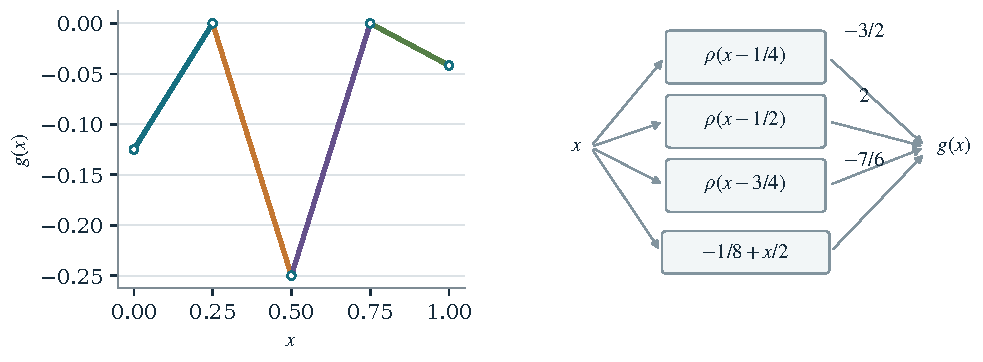
\includegraphics[width=1\linewidth]{figuras/artigo_1/04_relu.pdf}
\caption{Uma montagem racional com quatro folhas e a rede ReLU rasa dada pela identidade \eqref{artigo_1:eq:24}. O gráfico e os pesos são calculados a partir dos mesmos dados racionais.}\label{artigo_1:fig:relu}\end{figure}
A identidade funcional do teorema~4.3 conduz aos formatos da \cref{artigo_2:subsec:coding-formats}, que distinguem a transmissão estrutural dos diádicos de sua expansão em frações reduzidas.

\subsection{Relação com o 1-jato de Taylor}
Se $J_{k,m}$ tem centro $x_0$ e largura $h$, o 1-jato de $f\in C^2(J_{k,m})$ é
\[
T_{x_0}f(x)=f(x_0)+f'(x_0)(x-x_0).
\]
% MAPA artigo_1:4.5 | fonte artigos/artigo_1/secoes/04_montagens.tex:75
\begin{proposicao}[pertencimento e aderência]\label{map:artigo_1:4.5}
Se $f(x_0)\in\Q$ e $f'(x_0)\in\Q^*$, então $T_{x_0}f$ é o átomo de $\LL$ associado à célula. Em geral, para todo $\delta>0$ existem $q_0\in\Q$ e $q_1\in\Q^*$ tais que $\ell_q(x)=q_0+q_1(x-x_0)$ satisfaz
\eqn{28}{\normK{T_{x_0}f-\ell_q}{J_{k,m}}<\delta,}
\eqn{29}{\normK{f-\ell_q}{J_{k,m}}\le\frac{h^2}8\normK{f''}{J_{k,m}}+\delta.}
\end{proposicao}
\begin{proof}
No primeiro caso, $(x_0,f(x_0),f'(x_0))$ pertence ao contradomínio do teorema~3.6. No caso geral, escolha $q_0$ com $|f(x_0)-q_0|<\delta/2$ e $q_1\ne0$ com $|f'(x_0)-q_1|<\delta/h$. Como $|x-x_0|\le h/2$, obtém-se \eqref{artigo_1:eq:28}. O resto integral de Taylor fornece
\[
|f(x)-T_{x_0}f(x)|=\left|\int_{x_0}^x(x-t)f''(t)\,dt\right|
\le\frac{|x-x_0|^2}2\norm{f''}\le\frac{h^2}8\norm{f''}.
\]
A desigualdade triangular prova \eqref{artigo_1:eq:29}.
\end{proof}
Jatos reais arbitrários pertencem, portanto, à aderência local da biblioteca racional.
% FIM artigos/artigo_1/secoes/04_montagens.tex
% INICIO artigos/artigo_1/secoes/05_taxas.tex
\section{Taxas uniformes e constante assintótica}
Para $f\in C^2[\alpha,\beta]$, use a extensão
\eqn{30}{F(x)=\begin{cases}
f(\alpha)+f'(\alpha)(x-\alpha)+\frac12f''(\alpha)(x-\alpha)^2,&x<\alpha,\\
f(x),&\alpha\le x\le\beta,\\
f(\beta)+f'(\beta)(x-\beta)+\frac12f''(\beta)(x-\beta)^2,&x>\beta.
\end{cases}}
Então $F\in C^2(\R)$ e $\normK{F''}{\R}=\normK{f''}{[\alpha,\beta]}$. Seja $P_kF$ o interpolante nos nós $j2^{-k}$.

% MAPA artigo_1:5.1 | fonte artigos/artigo_1/secoes/05_taxas.tex:10
\begin{teorema}[cota aguda e limite]\label{map:artigo_1:5.1}
Ponha $h=2^{-k}$ e $M=\normK{f''}{[\alpha,\beta]}$. Então
\eqn{31}{\normK{f-P_kF}{[\alpha,\beta]}\le\frac{h^2M}8,}
e
\eqn{32}{\lim_{k\to\infty}\frac8{h^2}\normK{f-P_kF}{[\alpha,\beta]}=M.}
Além disso, para todo $\delta>0$ existe $g_{k,\delta}\in\Asm([\alpha,\beta])$ com
\eqn{33}{\norm{f-g_{k,\delta}}\le\frac{h^2M}8+\delta.}
\end{teorema}
\begin{proof}
Em uma célula $[x_L,x_R]$ de largura $h$, ponha $e=F-P_kF$. Para $x\in(x_L,x_R)$, a função
\[
\psi(t)=e(t)-\frac{(t-x_L)(t-x_R)}{(x-x_L)(x-x_R)}e(x)
\]
anula-se em $x_L,x,x_R$. Três aplicações de Rolle produzem $\xi_x\in(x_L,x_R)$ com $\psi''(\xi_x)=0$; portanto
\eqn{34}{F(x)-P_kF(x)=\frac12F''(\xi_x)(x-x_L)(x-x_R).}
O módulo do produto é no máximo $h^2/4$, com igualdade no centro, o que prova \eqref{artigo_1:eq:31}.

Se $M=0$, \eqref{artigo_1:eq:32} é imediata. Se $M>0$, escolha $x_*\in[\alpha,\beta]$ com $|f''(x_*)|=M$. Para cada $k$ suficientemente grande, escolha um centro de escala $k$, $z_k\in[\alpha,\beta]$, com $z_k\to x_*$. Avaliando \eqref{artigo_1:eq:34} em $z_k$,
\[
|F(z_k)-P_kF(z_k)|=\frac{h^2}8|F''(\xi_k)|,
\]
onde $\xi_k$ pertence à célula de $z_k$. O diâmetro da célula tende a zero, logo $\xi_k\to x_*$ e $|F''(\xi_k)|\to M$. Isso dá o limite inferior; \eqref{artigo_1:eq:31} fornece o superior.

Para a última afirmação, racionalize todos os valores nodais da cobertura finita com erro menor que $\delta$ e mantenha valores adjacentes distintos, como no teorema~4.2. O interpolante resultante é uma montagem e dista menos que $\delta$ de $P_kF$ em norma uniforme. A desigualdade triangular conclui.
\end{proof}

% MAPA artigo_1:5.2 | fonte artigos/artigo_1/secoes/05_taxas.tex:36
\begin{corolario}[preservação da constante]\label{map:artigo_1:5.2}
Existe uma sequência $g_k\in\Asm([\alpha,\beta])$ tal que
\[
\lim_{k\to\infty}\frac8{h^2}\norm{f-g_k}=M.
\]
\end{corolario}
\begin{proof}
Na construção do teorema~5.1, escolha erros nodais $\delta_k=o(h^2)$. Então
\[
\left|\norm{f-g_k}-\norm{f-P_kF}\right|\le\norm{g_k-P_kF}<\delta_k.
\]
Divida por $h^2/8$ e aplique \eqref{artigo_1:eq:32}.
\end{proof}
Com $N_k$ de \eqref{artigo_1:eq:23}, $h=(\beta-\alpha)N_k^{-1}(1+O(N_k^{-1}))$ e, portanto,
\eqn{35}{\norm{f-P_kF}\le\frac{(\beta-\alpha)^2M}8N_k^{-2}\bigl(1+O(N_k^{-1})\bigr).}
Quando os extremos já são nós da malha, o termo de borda desaparece.
\begin{table}[!htbp]\centering
\caption{Erro exato do interpolante de $e^x$ em $[0,1]$.}
\begin{tabular}{rrrr}\toprule
$k$&erro exato&$2^{-2k}e/8$&razão\\\midrule
2&$1{,}8774\times10^{-2}$&$2{,}1237\times10^{-2}$&$0{,}8840$\\
4&$1{,}2866\times10^{-3}$&$1{,}3273\times10^{-3}$&$0{,}9693$\\
6&$8{,}2310\times10^{-5}$&$8{,}2955\times10^{-5}$&$0{,}9922$\\
8&$5{,}1746\times10^{-6}$&$5{,}1847\times10^{-6}$&$0{,}9980$\\
10&$3{,}2389\times10^{-7}$&$3{,}2404\times10^{-7}$&$0{,}9995$\\\bottomrule
\end{tabular}
\end{table}
\begin{figure}[!htbp]\centering
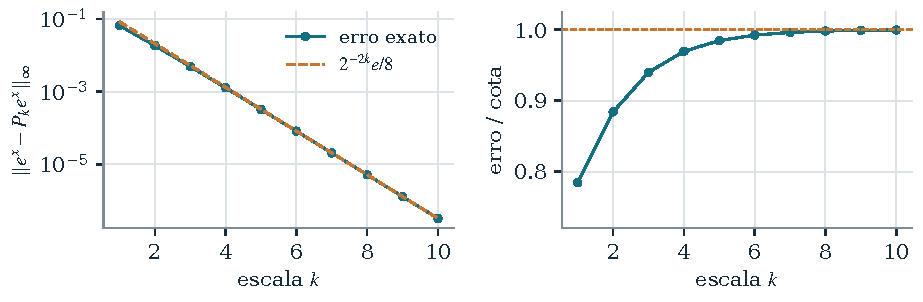
\includegraphics[width=.98\linewidth]{figuras/artigo_1/05_taxa_exponencial.pdf}
\caption{Erro do interpolante de $e^x$ e razão entre erro e cota. A razão converge a $1$, conforme \eqref{artigo_1:eq:32}.}\label{artigo_1:fig:taxa}\end{figure}
% FIM artigos/artigo_1/secoes/05_taxas.tex
% INICIO artigos/artigo_1/secoes/06_refinamento.tex
\section{Refinamento diádico adaptativo certificado}
O refinamento usa majorantes locais validados de $|F''|$ para controlar o erro em cada célula.

\subsection{Fechamento operacional por aritmética intervalar}
Seja $\EE$ a menor classe de expressões que contém $x$ e as constantes racionais e é fechada por soma, subtração, produto, recíproco, $\exp$, $\sin$, $\cos$ e composição. Um recíproco é admissível em intervalos nos quais seu denominador não se anula. Essa classe contém os polinômios, as funções racionais sem polos no domínio e as funções elementares usadas nos exemplos.

Composição significa substituição sintática: em $u\circ v$, cada folha $x$ da árvore de $u$ é substituída pela árvore de $v$. Toda expressão composta é, assim, uma árvore das operações-base.

Escreva $\mathbb I_{\Q}$ para os intervalos fechados com extremos racionais. A rotina
\eqn{36}{\operatorname{BoundSecondDerivative}(E,J;P,d)
=[\underline m_J,\overline m_J]\in\mathbb I_{\Q}}
usa precisão transcendental $P$ e profundidade de subdivisão $d$. Ela propaga simultaneamente intervalos para $(E,E',E'')$, isto é, 2-jatos intervalares. Por exemplo,
\begin{align*}
(uv)''&=u''v+2u'v'+uv'',\\
(u^{-1})''&=2(u')^2u^{-3}-u''u^{-2},\\
(e^u)''&=e^u\bigl((u')^2+u''\bigr),\\
(\sin u)''&=-\sin(u)(u')^2+\cos(u)u'',\\
(\cos u)''&=-\cos(u)(u')^2-\sin(u)u''.
\end{align*}
As operações racionais são exatas. Para $\exp$, a redução do argumento a $|z|\le1/2$ é seguida por uma soma de Taylor com resto majorado por uma série geométrica racional; para $\sin$ e $\cos$, usa-se o resto de Lagrange racional e a interseção com $[-1,1]$. Elevar $P$ e $d$ reduz a sobrestimação.

% MAPA artigo_1:6.1 | fonte artigos/artigo_1/secoes/06_refinamento.tex:22
\begin{lema}[restos transcendentais com extremos racionais]\label{map:artigo_1:6.1}
Se $I=[a,b]\in\mathbb I_{\Q}$, as rotinas descritas acima produzem intervalos de extremos racionais que contêm $\exp(I)$, $\sin(I)$ e $\cos(I)$. Mais explicitamente, para $0\le z\le1/2$ e $n\ge0$,
\eqn{37}{0\le e^z-\sum_{j=0}^n\frac{z^j}{j!}
\le\frac{z^{n+1}}{(n+1)!}\frac1{1-z/(n+2)}.}
Se $R=\max\{|a|,|b|\}$ e
\[
P_n^{\sin}(z)=\sum_{j=0}^n(-1)^j\frac{z^{2j+1}}{(2j+1)!},\qquad
P_n^{\cos}(z)=\sum_{j=0}^n(-1)^j\frac{z^{2j}}{(2j)!},
\]
então, para todo $z\in I$,
\eqn{38}{|\sin z-P_n^{\sin}(z)|\le\frac{R^{2n+2}}{(2n+2)!},\qquad
|\cos z-P_n^{\cos}(z)|\le\frac{R^{2n+1}}{(2n+1)!}.}
Avaliar os polinômios em $I$, inflar pelos respectivos restos e intersectar com $[-1,1]$ preserva a inclusão.
\end{lema}
\begin{proof}
Na série de $e^z$, o primeiro termo omitido é $t_{n+1}=z^{n+1}/(n+1)!$. Para $j\ge n+1$, a razão entre termos consecutivos é $z/(j+1)\le z/(n+2)<1$; a cauda é, portanto, majorada pela série geométrica de primeiro termo $t_{n+1}$ e razão $z/(n+2)$, o que dá \eqref{artigo_1:eq:37}. Para um argumento racional $x$ arbitrário, escolha $r$ com $z=|x|/2^r\le1/2$, aplique a inclusão anterior e eleve o intervalo ao quadrado $r$ vezes; se $x<0$, tome o recíproco do intervalo positivo obtido para $-x$. Em $I=[a,b]$, a monotonicidade de $e^x$ permite usar o extremo inferior da inclusão em $a$ e o superior da inclusão em $b$.

As duas desigualdades em \eqref{artigo_1:eq:38} são o resto de Lagrange dos polinômios de Maclaurin de graus $2n+1$ e $2n$, pois todas as derivadas de seno e cosseno têm módulo no máximo $1$. A avaliação intervalar contém a imagem de cada polinômio; inflar pelo raio do resto contém a função. Como seno e cosseno já pertencem a $[-1,1]$, a interseção não remove nenhum valor possível. Todas as operações, fatoriais e extremos envolvidos são racionais.
\end{proof}

% MAPA artigo_1:6.2 | fonte artigos/artigo_1/secoes/06_refinamento.tex:42
\begin{proposicao}[correção do majorante intervalar]\label{map:artigo_1:6.2}
Se $E\in\EE$ define uma função $C^2$ em $J$ e a rotina \eqref{artigo_1:eq:36} termina com sucesso, então
\eqn{39}{E''(x)\in[\underline m_J,\overline m_J]\ (x\in J),\qquad
M_{\rm int}(J):=\max\{|\underline m_J|,|\overline m_J|\}\ge\normK{E''}{J}.}
Se algum intervalo de denominador contém zero mesmo após a subdivisão permitida, a rotina devolve falha e nenhum número é aceito como certificado.
\end{proposicao}
\begin{proof}
Para constantes e para $x$, a inclusão é imediata. Soma, produto e recíproco preservam inclusão pelas operações elementares de intervalos; o recíproco só é executado quando zero está fora do intervalo do denominador. As fórmulas de 2-jatos acima e o lema~6.1 dão o passo de indução estrutural para toda expressão de $\EE$. Pela normalização sintática declarada antes do lema, uma composição genérica já foi expandida nessa árvore e não acrescenta um caso independente. Subdividir $J$ preserva a cobertura, e tomar o fecho convexo dos intervalos obtidos em suas partes contém a união das imagens de $E''$. Isso prova a primeira inclusão e, tomando módulos, \eqref{artigo_1:eq:39}. A regra de falha impede que uma divisão não validada produza uma falsa garantia.
\end{proof}
A propagação registra a largura dos intervalos, o número de caixas e a profundidade usados. Subdivisão e Taylor racional permitem apertar as inclusões.

% MAPA artigo_1:6.3 | fonte artigos/artigo_1/secoes/06_refinamento.tex:53
\begin{algoritmo}[refinamento certificado]\label{map:artigo_1:6.3}
Dados $f\in C^2[\alpha,\beta]$, tolerâncias $\varepsilon_I,\varepsilon_R>0$ e a extensão $F$ de \eqref{artigo_1:eq:30}, use, para toda célula $J$, um majorante validado
\eqn{40}{\normK{F''}{J}\le M(J)\le M_*<\infty.}
Quando $F$ é fornecida por uma expressão de $\EE$, tome $M(J)=M_{\rm int}(J)$ de \eqref{artigo_1:eq:39}; se a certificação falhar, aborte sem emitir uma montagem garantida. Para uma função $C^2$ fora dessa interface, \eqref{artigo_1:eq:40} é um contrato de entrada.
\begin{enumerate}[label=(\roman*),topsep=6pt,itemsep=3pt]
\item Inicie com uma cobertura diádica finita de $[\alpha,\beta]$.
\item Para cada folha $J$, calcule
\eqn{41}{\eta_{\rm cert}(J)=\frac{|J|^2M(J)}8.}
\item Enquanto existir folha com $\eta_{\rm cert}(J)>\varepsilon_I$, substitua-a por seus dois filhos.
\item Nos nós finais, escolha racionais compartilhados $v_t$ com $|v_t-F(t)|<\varepsilon_R$ e valores adjacentes distintos.
\item Emita, em cada folha, o endereço do átomo que interpola seus dois valores nodais.
\end{enumerate}
\end{algoritmo}

% MAPA artigo_1:6.4 | fonte artigos/artigo_1/secoes/06_refinamento.tex:67
\begin{teorema}[correção, término e tamanho]\label{map:artigo_1:6.4}
O algoritmo~6.3 termina e produz $g\in\Asm([\alpha,\beta])$ com
\eqn{42}{\norm{f-g}\le\varepsilon_I+\varepsilon_R.}
Se a cobertura inicial tem $R_0$ raízes de largura máxima $h_0$ e $M_*>0$, nenhuma ramificação ultrapassa
\eqn{43}{r_*=\max\left\{0,\left\lceil\frac12\log_2\left(\frac{h_0^2M_*}{8\varepsilon_I}\right)\right\rceil\right\}}
níveis, e há no máximo $R_02^{r_*}$ folhas. Se $M_*=0$, pode-se tomar $r_*=0$.
\end{teorema}
\begin{proof}
Após $r$ subdivisões, uma folha descendente de uma raiz tem $|J|\le h_02^{-r}$ e, por \eqref{artigo_1:eq:40},
\[
\eta_{\rm cert}(J)\le\frac{h_0^2M_*}8\,4^{-r}.
\]
O lado direito é no máximo $\varepsilon_I$ para $r\ge r_*$; logo nenhuma folha é subdividida além dessa profundidade. A árvore é finita e cada raiz gera no máximo $2^{r_*}$ folhas.

Na partição final, \eqref{artigo_1:eq:34} e \eqref{artigo_1:eq:40} implicam
\[
\normK{F-P_\Lambda F}{J}\le\frac{|J|^2}8\normK{F''}{J}\le\eta_{\rm cert}(J)\le\varepsilon_I.
\]
A racionalização nodal produz, pelos teoremas~3.5 e 3.6, uma montagem de átomos de endereço único e com $\norm{P_\Lambda F-g}<\varepsilon_R$. Como $F=f$ no intervalo original, a desigualdade triangular prova \eqref{artigo_1:eq:42}.
\end{proof}
\begin{figure}[H]\centering
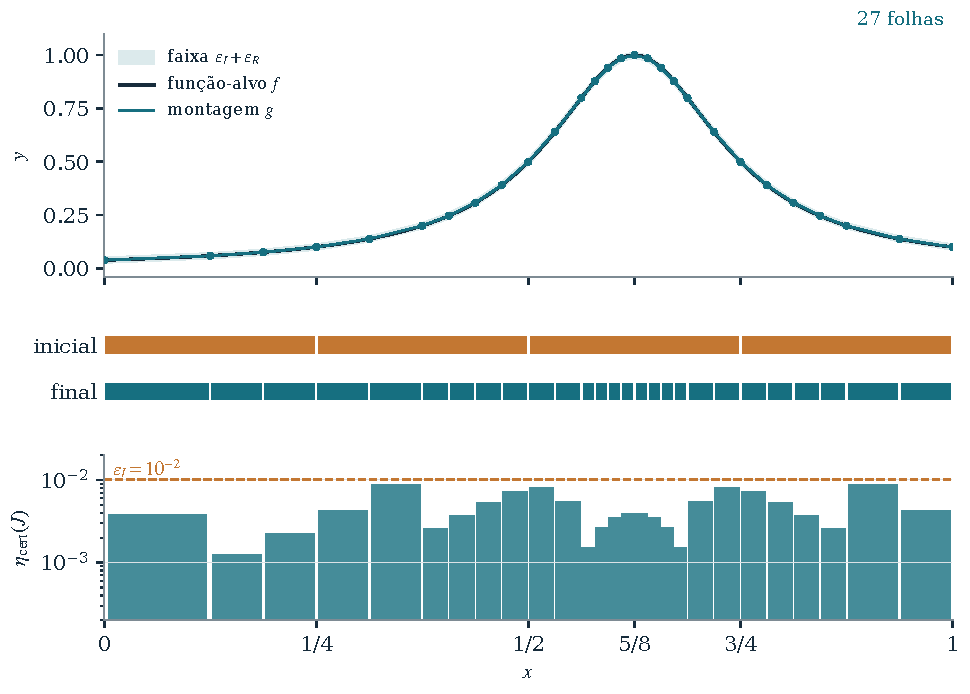
\includegraphics[width=.90\linewidth]{figuras/artigo_1/06_refinamento_certificado.pdf}
\caption{Refinamento certificado para $f(x)=[1+64(x-5/8)^2]^{-1}$. Células com certificado acima de $\varepsilon_I$ são subdivididas. A malha se concentra na região de maior curvatura, e o painel inferior compara os certificados finais com a tolerância. A faixa superior representa o limite uniforme $\varepsilon_I+\varepsilon_R$.}
\label{artigo_1:fig:refinamento}
\end{figure}

% MAPA artigo_1:6.5 | fonte artigos/artigo_1/secoes/06_refinamento.tex:93
\begin{proposicao}[calibração exata para curvatura constante]\label{map:artigo_1:6.5}
Suponha que $[\alpha,\beta]=J_0$ seja uma única célula diádica inicial, $F''\equiv\kappa\ne0$ em $J_0$ e $M(J)=|\kappa|$ em todo descendente. Pondo
\[
A=\frac{|J_0|^2|\kappa|}8,
\]
o número de folhas produzido com tolerância $\varepsilon_I$ é
\eqn{44}{N(\varepsilon_I)=2^{r(\varepsilon_I)},\qquad
r(\varepsilon_I)=\max\left\{0,\left\lceil\log_4\left(\frac A{\varepsilon_I}\right)\right\rceil\right\}.}
Consequentemente,
\eqn{45}{\begin{aligned}
\liminf_{\varepsilon_I\downarrow0}\sqrt{\varepsilon_I}\,N(\varepsilon_I)
&=\frac1{\sqrt8}\int_\alpha^\beta|f''(x)|^{1/2}\,dx,\\
\limsup_{\varepsilon_I\downarrow0}\sqrt{\varepsilon_I}\,N(\varepsilon_I)
&=\frac1{\sqrt2}\int_\alpha^\beta|f''(x)|^{1/2}\,dx.
\end{aligned}}
A quantização diádica introduz, nesse caso, um fator dois entre os limites de acumulação.
\end{proposicao}
\begin{proof}
Após $r$ subdivisões uniformes, cada folha tem largura $|J_0|2^{-r}$ e certificado $A4^{-r}$. Como todos os certificados de um mesmo nível são iguais, o algoritmo para no primeiro $r$ com $A4^{-r}\le\varepsilon_I$, o que prova \eqref{artigo_1:eq:44}. Para $A4^{-r}\le\varepsilon_I<A4^{-(r-1)}$, tem-se
\[
\sqrt A\le\sqrt{\varepsilon_I}\,2^r<2\sqrt A.
\]
Os extremos inferior e superior são atingidos, respectivamente, nos limiares $\varepsilon_I=A4^{-r}$ e por aproximação pela esquerda aos limiares $A4^{-(r-1)}$. Por fim, $\int_\alpha^\beta|f''|^{1/2}=|J_0|\sqrt{|\kappa|}$.
\end{proof}

% MAPA artigo_1:6.6 | fonte artigos/artigo_1/secoes/06_refinamento.tex:118
\begin{observacao}[diferença segunda e erro no centro]\label{map:artigo_1:6.6}
Se $x_0=(x_L+x_R)/2$, então
\[
|f(x_0)-P_Jf(x_0)|=\frac12|f(x_L)-2f(x_0)+f(x_R)|.
\]
Isso mede o erro no centro. Para $f(x)=x^3$ em $[-1,1]$, $P_Jf(x)=x$ e a diferença segunda central é zero, enquanto
\[
\norm{x^3-x}=\frac2{3\sqrt3}\approx0{,}3849.
\]
O controle em todo o intervalo é fornecido pelo majorante de \eqref{artigo_1:eq:40}.
\end{observacao}
% FIM artigos/artigo_1/secoes/06_refinamento.tex
% INICIO artigos/artigo_1/secoes/08_conclusao.tex
\begin{figure}[!htbp]
\centering
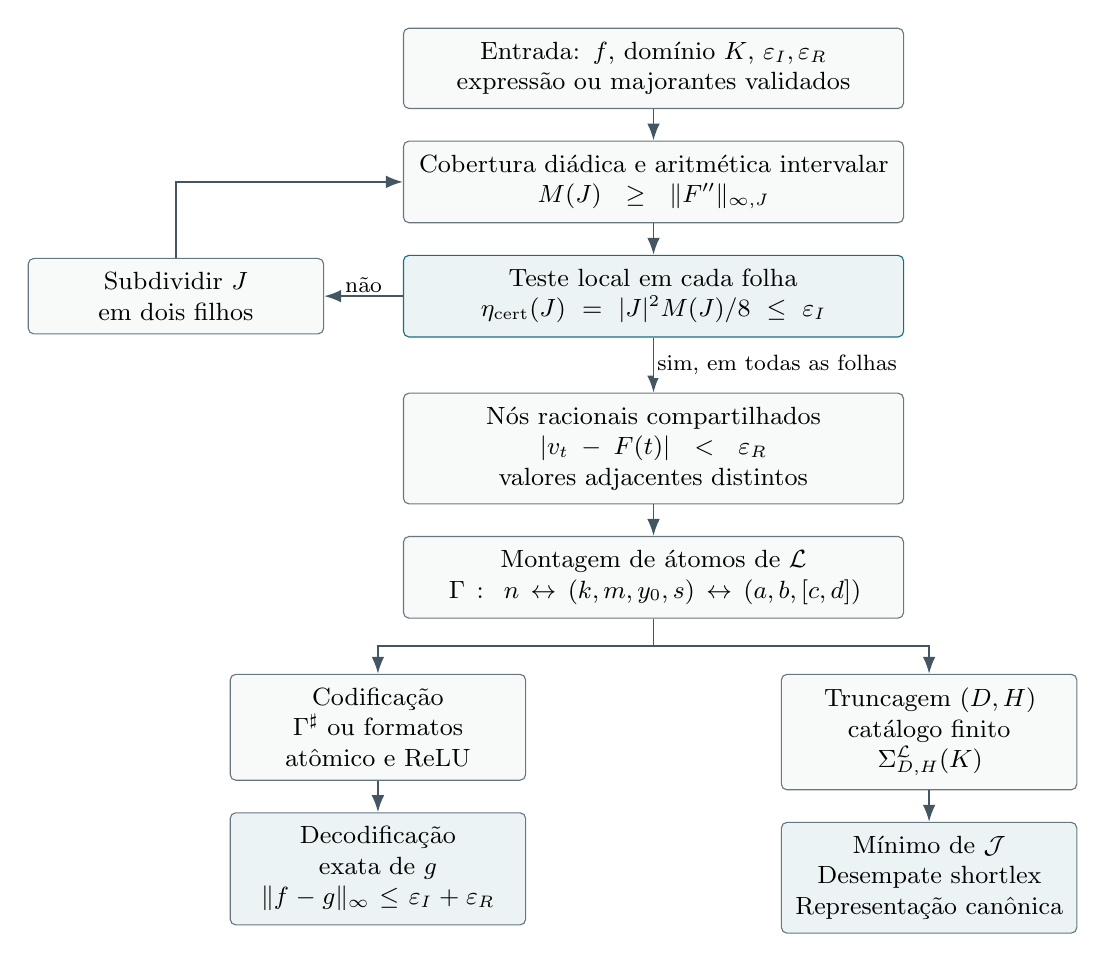
\begin{tikzpicture}[
 >=Latex,
 box/.style={draw=ink!65,rounded corners=2pt,fill=ink!3,
  align=center,text width=6.0cm,minimum height=.95cm,inner sep=5pt,font=\small},
 side/.style={box,text width=3.4cm},
 arr/.style={->,line width=.7pt,draw=ink!80},
 lab/.style={font=\footnotesize,fill=white,inner sep=1pt}]
\node[box] (in) {Entrada: $f$, domínio $K$, $\varepsilon_I,\varepsilon_R$\\expressão ou majorantes validados};
\node[box,below=4mm of in] (bound) {Cobertura diádica e aritmética intervalar\\$M(J)\ge\|F''\|_{\infty,J}$};
\node[box,below=4mm of bound,fill=accent!8,draw=accent] (test)
 {Teste local em cada folha\\$\eta_{\rm cert}(J)=|J|^2M(J)/8\le\varepsilon_I$};
\node[side,left=10mm of test] (split) {Subdividir $J$\\em dois filhos};
\node[box,below=7mm of test] (rational) {Nós racionais compartilhados\\$|v_t-F(t)|<\varepsilon_R$\\valores adjacentes distintos};
\node[box,below=4mm of rational] (atoms) {Montagem de átomos de $\LL$\\$\Gamma:\ n\leftrightarrow(k,m,y_0,s)\leftrightarrow(a,b,[c,d])$};
\node[side,anchor=north] (codec) at ($(atoms.south)+(-3.5,-.7)$)
 {Codificação\\$\Gamma^\sharp$ ou formatos\\atômico e ReLU};
\node[side,anchor=north] (catalog) at ($(atoms.south)+(3.5,-.7)$)
 {Truncagem $(D,H)$\\catálogo finito\\$\Sigma^{\LL}_{D,H}(K)$};
\node[side,below=4mm of codec,fill=accent!8] (out)
 {Decodificação exata de $g$\\$\|f-g\|_\infty\le\varepsilon_I+\varepsilon_R$};
\node[side,below=4mm of catalog,fill=accent!8] (min)
 {Mínimo de $\mathcal J$\\Desempate shortlex\\Representação canônica};
\draw[arr] (in)--(bound);
\draw[arr] (bound)--(test);
\draw[arr] (test.west)--node[lab,above]{não}(split.east);
\draw[arr] (split.north)|-(bound.west);
\draw[arr] (test)--node[lab,right]{sim, em todas as folhas}(rational);
\draw[arr] (rational)--(atoms);
\draw[arr] (atoms.south)--++(0,-.35)-|(codec.north);
\draw[arr] (atoms.south)--++(0,-.35)-|(catalog.north);
\draw[arr] (codec)--(out);
\draw[arr] (catalog)--(min);
\end{tikzpicture}
\caption{Circuito da construção: certificação local, refinamento, racionalização, endereçamento e descrição. A truncagem fornece a via finita de enumeração e minimização.}
\label{artigo_1:fig:circuito}
\end{figure}

\section{Conclusão}
A biblioteca $\LL$ reúne segmentos afins racionais com endereço único e suporte diádico recuperável. A bijeção com jatos racionais produz montagens contínuas densas em $C(K)$ e uma representação ReLU rasa exata. Na aproximação uniforme de funções $C^2$, a racionalização preserva a constante $1/8$ do erro interpolatório.

O refinamento adaptativo combina majorantes intervalares da segunda derivada e racionalização nodal para obter erro até $\varepsilon_I+\varepsilon_R$, com término e número de folhas controlados sob as hipóteses declaradas. A contagem aritmética, a codificação e a seleção exata são desenvolvidas no segundo artigo; as agendas de altura e a teoria direta--inversa, no terceiro. Os quatro resultados de referência não reproduzidos nesses recortes têm texto e demonstração preservados no complemento do original.
% FIM artigos/artigo_1/secoes/08_conclusao.tex
\clearpage
\section*{Apêndice da Parte I}\addcontentsline{toc}{section}{Apêndice da Parte I}
\setcounter{section}{0}\renewcommand{\thesection}{I.\Alph{section}}
% INICIO artigos/artigo_1/secoes/A_notacao.tex
\section{Quadro de notação}
\footnotesize
\renewcommand{\arraystretch}{1.1}
\begin{longtable}{@{}p{.28\linewidth}p{.68\linewidth}@{}}
\toprule Símbolo&Significado\\\midrule
\endfirsthead
\toprule Símbolo&Significado\\\midrule
\endhead
\bottomrule\endfoot
$\pi,\pi^{-1}$&Pareamento de Cantor e sua inversa.\\
$Z,Q,Q^*$&Enumerações de $\Z$, $\Q$ e $\Q^*$.\\
$\heightq(p/q)$&Altura $\max\{|p|,q\}$ da fração reduzida.\\
$\Q_H$&Racionais de altura no máximo $H$.\\
$\D,\D_{\rm mid}$&Diádicos e diádicos não inteiros.\\
$J_{k,m},J_{k,m}^{\rm own}$&Célula fechada e célula semiaberta de posse.\\
$x_0,y_0,s$&Centro, valor ancorado e inclinação de um átomo.\\
$\Gamma,\LL,\LL_H$&Gerador aritmético, biblioteca e truncagem por altura.\\
$I_n^x$&Suporte espacial recuperado da interface global.\\
$\Asm(K)$&Montagens contínuas finitas no domínio $K$.\\
$\omega(f;\delta)$&Módulo de continuidade de $f$.\\
$\rho(z)=z_+$&Ativação ReLU.\\
$P_kF,P_Jf,P_\Lambda F$&Interpolantes na malha uniforme, em uma célula e em uma partição.\\
$\EE,\mathbb I_{\Q}$&Gramática de expressões e intervalos de extremos racionais.\\
$P,d$&Precisão transcendental e profundidade de subdivisão intervalar.\\
$M_{\rm int}(J),M(J)$&Majorantes validados de $\|F''\|_{\infty,J}$.\\
$\eta_{\rm cert}(J)$&Certificado local $|J|^2M(J)/8$.\\
$\varepsilon_I,\varepsilon_R$&Tolerâncias de interpolação e racionalização.\\
$H$&Calibre atômico definido em \eqref{artigo_1:eq:46}.\\
\end{longtable}
\normalsize
% FIM artigos/artigo_1/secoes/A_notacao.tex


% II | fonte original: entradas/parte_1/Solucao_Equivalencia_Montagens_Parte_1 (1).tex
\volumeparte{Normalização e equivalência das montagens}
% Reconstruído de entradas/parte_1/Solucao_Equivalencia_Montagens_Parte_1 (1).tex



\begin{abstract}
Fixamos os tipos e as dependências de todas as construções usadas na
normalização de montagens diádicas. Definimos as representações por
átomos e por células endereçadas, suas conversões, as classes de funções,
os orçamentos e os erros em um reticulado completo. Demonstramos a
normalização por células ativas e a equivalência entre as três
formulações com os mesmos limites de folhas e altura. A ordenação finita,
a cadeia de nós e a extensão ReLU recebem construções explícitas. As
operações recursivas incluem medidas de término e casos iniciais.
\end{abstract}

\section{Base de tipos e convenções}
\label{normalizacao:sec:base}

\paragraph{Primitivos.}
Usamos os tipos padrão $\N=\{0,1,\ldots\}$, $\Z$, $\Q$ e $\R$,
as inclusões canônicas entre eles, conjuntos, subtipos, funções,
produtos, listas e conjuntos finitos. Em Lean, correspondem aos tipos
padrão e às estruturas de \code{Mathlib}. A ordem e a topologia de $\R$
são as usuais. Soma, produto, potência natural, mínimo, máximo,
continuidade, fecho, interior e cardinalidade finita têm suas definições
padrão nessa biblioteca. Os objetos próprios deste desenvolvimento são
definidos abaixo em ordem de dependência.

\paragraph{Subtipos e igualdade.}
Para $P:X\to\mathrm{Prop}$, o subtipo
$\{x:X\mid P(x)\}$ contém pares $\langle x,h\rangle$, com $h:P(x)$.
Sua projeção é $\langle x,h\rangle\mapsto x$. Dois elementos desse subtipo
são iguais quando suas projeções são iguais; as provas não constituem
dados adicionais de comparação. A igualdade de funções é extensional.

\paragraph{Conjuntos finitos.}
$\FS(X)$ é o tipo dos conjuntos finitos de elementos de $X$, sem
multiplicidades. Para $F:\FS(X)$, escrevemos $x\in F$ para pertinência e
$|F|:=\card F\in\N$. Fixamos as operações
\begin{align*}
 \operatorname{filter}(P,F)&=\{x\in F:P(x)\},\\
 \operatorname{image}(u,F)&=\{u(x):x\in F\},\\
 \operatorname{erase}(F,x)&=F\setminus\{x\}.
\end{align*}
São caracterizadas por essas equivalências de pertinência. Em particular,
filtrar produz um subconjunto, e a imagem por uma função injetiva em $F$
preserva $|F|$. Escrever $\bigcup_{x\in F}S_x$ significa o conjunto
$\{z:\exists x\in F,\ z\in S_x\}$. A finitude é mantida como dado, e
não como uma hipótese implícita sobre um conjunto arbitrário.
O conjunto subjacente a $F$ é $\{x:X:x\in F\}$.
Se $S\subseteq X$ é um conjunto finito com esse mesmo conjunto
subjacente, sua cardinalidade natural $S.\operatorname{ncard}$ é $|F|$.
Isso identifica contagens por conjuntos finitos e por \code{Finset}
quando as implementações dos postos usam representações diferentes.

\paragraph{Índices finitos.}
$\Fin(n):=\{j:\N\mid j<n\}$. Quando escrevemos $a_j$ para
$a:\Fin(n)\to X$, a desigualdade $j<n$ faz parte do índice.
Denote por $\operatorname{univ}_n:\FS(\Fin(n))$ o conjunto de todos
os elementos de $\Fin(n)$. Uma soma $\sum_{1\le j<M}$ percorre o conjunto finito
$\{j:\N:1\le j<M\}$; nela, $j$ e $j-1$ são índices válidos de
$\Fin(M)$. Se $M=1$, esse conjunto é vazio e a soma vale zero.

\paragraph{Domínio.}
Fixe $\alpha,\beta:\R$ e uma hipótese $h_K:\alpha<\beta$.
Defina separadamente o conjunto e o subtipo
\[
 K:=\{x:\R:\alpha\le x\le\beta\},\qquad
 |K|_{\rm type}:=\{x:\R\mid x\in K\},\qquad
 \iota_K:|K|_{\rm type}\to\R,\quad\iota_K(z)=z.1.
\]
Usamos $K$ também para o subtipo quando o tipo de uma função o explicita.
O intervalo aberto é $K^\circ=(\alpha,\beta)$.
Defina
\[
 \CK:=\{g:K\to\R\mid g\text{ é contínua na topologia de subtipo}\}.
\]
Para espaços topológicos $X,Y$, $C(X,Y)$ denota funções contínuas
com domínio $X$ e codomínio $Y$, acompanhadas da prova de continuidade.
Assim $\CK=C(K,\R)$ é o tipo
\code{ContinuousMap (Set.Icc alpha beta) Real}. Para $g:\CK$ e $x\in K$, a expressão $g(x)$ abrevia
$g(\langle x,h_x\rangle)$; seu valor independe da prova $h_x$.
O domínio é não vazio, compacto e igual a $\cls(K^\circ)$.

\section{Racionais, células e átomos}
\label{normalizacao:sec:objects}

% MAPA normalizacao:2.1
\begin{definicao}[racional reduzido e altura]\label{map:normalizacao:2.1}
Para $r:\Q$, sejam $p(r):\Z$ e $q(r):\N$ seu numerador e denominador
reduzidos, determinados por
\[
 q(r)>0,\qquad \gcd(|p(r)|,q(r))=1,\qquad r=p(r)/q(r).
\]
Em particular, $p(0)=0$ e $q(0)=1$. Defina
\[
 \htq:\Q\to\N,\qquad \htq(r)=\max\{|p(r)|,q(r)\},\qquad
 \qstar:=\{r:\Q\mid r\ne0\}.
\]
Aqui $|p(r)|$ é o valor absoluto natural do inteiro, isto é,
\code{Rat.num.natAbs}; $q(r)$ é \code{Rat.den}. Logo
$1\le\htq(r)$, $|p(r)|\le\htq(r)$ e $q(r)\le\htq(r)$.
\end{definicao}

% MAPA normalizacao:2.2
\begin{definicao}[célula e funções de seus extremos]\label{map:normalizacao:2.2}
O tipo de índices de células é $\Cell:=\N\times\Z$. Para $c=(k,m)$,
defina primeiro funções com valores racionais:
\begin{align*}
 L_\Q(c)&=\frac{m}{2^k},&
 R_\Q(c)&=\frac{m+1}{2^k},&
 X_\Q(c)&=\frac{2m+1}{2^{k+1}}.
\end{align*}
As operações nessas fórmulas são em $\Q$. Defina as versões reais por
inclusão: $L(c)=\uparrow L_\Q(c)$, $R(c)=\uparrow R_\Q(c)$ e
$X(c)=\uparrow X_\Q(c)$. Os três intervalos associados são
\[
 J(c)=[L(c),R(c)],\qquad O(c)=(L(c),R(c)),\qquad
 P(c)=[L(c),R(c)).
\]
$J(c)$ é o suporte fechado. $O(c)=\intr J(c)$ é seu interior.
$P(c)$ é a convenção de posse semiaberta; ela não substitui $J(c)$
nas definições de representação.
Os diádicos são
$\D:=\{\uparrow(m/2^k):(k,m)\in\Cell\}\subset\R$.
\end{definicao}

% MAPA normalizacao:2.3
\begin{lema}[geometria elementar]\label{map:normalizacao:2.3}\label{normalizacao:lem:geometry}
Para $c=(k,m)$,
\[
 R_\Q(c)-L_\Q(c)=2^{-k}>0,\qquad
 X_\Q(c)=\frac{L_\Q(c)+R_\Q(c)}2.
\]
Consequentemente, $J(c)$ é fechado e não degenerado, $O(c)$ é não
vazio e $L(c)<X(c)<R(c)$. Os três valores pertencem a $\D$.
Além disso, $J(c)=J(d)$ implica $c=d$.
\end{lema}
\begin{proof}
As duas identidades seguem da aritmética racional e $2^k>0$.
Para o centro, use o índice $(k+1,2m+1)$ na definição de $\D$.
Se os suportes são iguais, seus mínimos e máximos são iguais.
As larguras dão $2^{-k}=2^{-k'}$, logo $k=k'$, pela estrita
monotonicidade das potências de dois. A igualdade dos extremos
esquerdos dá então $m=m'$.
\end{proof}

% MAPA normalizacao:2.4
\begin{definicao}[átomo e suas projeções]\label{map:normalizacao:2.4}\label{normalizacao:def:atom}
$\Atoms$ é a estrutura com campos
\[
 k:\N,\quad m:\Z,\quad y:\Q,\quad s:\Q,\quad h_s:s\ne0.
\]
A igualdade de átomos é a igualdade dos quatro campos de dados
$(k,m,y,s)$. Para $a:\Atoms$, defina
\begin{align*}
 C(a)&=(a.k,a.m):\Cell, & J_a&=J(C(a)), & O_a&=O(C(a)),\\
 L_a&=L(C(a)),&R_a&=R(C(a)),&X_a&=X(C(a)),\\
 b(a)&=a.s:\Q,& u(a)&=a.y-a.s\,X_\Q(C(a)):\Q.
\end{align*}
\begin{align*}
 \ell_a(x)&=\uparrow a.y+\uparrow a.s\,(x-X_a)\quad(x:\R),\\
 h(a)&=\max\{2,a.k+1,|a.m|+1,\htq(a.y),\htq(a.s)\}:\N.
\end{align*}
O átomo de valor padrão é
$a_\dagger=(0,0,0,1,\,1\ne0)$.
\end{definicao}

% MAPA normalizacao:2.5
\begin{lema}[formas da reta]\label{map:normalizacao:2.5}\label{normalizacao:lem:line}
Para todo $a:\Atoms$ e $x:\R$,
\[
 \ell_a(x)=\uparrow u(a)+\uparrow b(a)\,x,\qquad
 \ell_a(X_a)=\uparrow a.y.
\]
A função $\ell_a:\R\to\R$ é contínua e tem inclinação não nula.
Se $C(a)=C(a')$, $a.y=a'.y$ e $a.s=a'.s$, então
$a=a'$, $J_a=J_{a'}$ e $\ell_a=\ell_{a'}$ como funções globais.
\end{lema}
\begin{proof}
Expanda os produtos, usando que a inclusão $\Q\to\R$ preserva soma
e produto. A continuidade é a de uma função afim. A inclusão é
injetiva, logo $h_s$ também garante a inclinação real não nula.
As igualdades finais seguem da igualdade dos campos da estrutura.
\end{proof}

\section{Predicados de representação e normalização}
\label{normalizacao:sec:normalization}

% MAPA normalizacao:3.1
\begin{definicao}[campos dos contratos]\label{map:normalizacao:3.1}\label{normalizacao:def:contracts}
Para $\Lambda:\FS(\Atoms)$, $g:\CK$ e $G:\R\to\R$, defina
\begin{align*}
 \Sep(\Lambda)&:\Longleftrightarrow
  \forall a,b\in\Lambda,\ a\ne b\Rightarrow O_a\cap O_b=\varnothing,\\
 \Cov(K,\Lambda)&:\Longleftrightarrow
  \forall x\in K,\ \exists a\in\Lambda,\ x\in J_a,\\
 \Match_K(g,\Lambda)&:\Longleftrightarrow
  \forall a\in\Lambda\ \forall z:K,\
       \iota_K(z)\in J_a\Rightarrow g(z)=\ell_a(\iota_K(z)),\\
 \Match^G_K(G,\Lambda)&:\Longleftrightarrow
  \forall a\in\Lambda\ \forall x\in J_a\cap K,\ G(x)=\ell_a(x),\\
 \Agree(\Lambda)&:\Longleftrightarrow
  \forall a,b\in\Lambda\ \forall x\in J_a\cap J_b,\
       \ell_a(x)=\ell_b(x).
\end{align*}
Defina os predicados, todos com valores em $\mathrm{Prop}$,
\begin{align*}
 \Loc_K(g,\Lambda)&:=\Sep(\Lambda)\land\Cov(K,\Lambda)
                         \land\Match_K(g,\Lambda),\\
 \Str_K(g,\Lambda)&:=\Loc_K(g,\Lambda)\land\Agree(\Lambda),\\
 \Loc^G_K(G,\Lambda)&:=\Sep(\Lambda)\land\Cov(K,\Lambda)
                         \land\Match^G_K(G,\Lambda),\\
 \Str^G_K(G,\Lambda)&:=\Loc^G_K(G,\Lambda)\land\Agree(\Lambda).
\end{align*}
Finalmente, como subconjuntos do mesmo tipo $\CK$,
\[
 \Aloc(K):=\{g:\CK:\exists\Lambda,\ \Loc_K(g,\Lambda)\},\qquad
 \Astr(K):=\{g:\CK:\exists\Lambda,\ \Str_K(g,\Lambda)\}.
\]
\end{definicao}

A igualdade das retas em $J_a\cap J_b\cap K$ é consequência de
$\Match$: ambas têm o valor $g(x)$. A cláusula $\Agree$ exige
igualdade também nos encontros fora de $K$.

% MAPA normalizacao:3.2
\begin{definicao}[atividade e filtro]\label{map:normalizacao:3.2}\label{normalizacao:def:norm}
Defina $\Act_K:\Atoms\to\mathrm{Prop}$ e
$\Norm_K:\FS(\Atoms)\to\FS(\Atoms)$ por
\[
 \Act_K(a):\Longleftrightarrow O_a\cap K^\circ\ne\varnothing,
 \qquad \Norm_K(\Lambda):=\operatorname{filter}(\Act_K,\Lambda).
\]
Portanto,
$a\in\Norm_K(\Lambda)\Longleftrightarrow a\in\Lambda\land\Act_K(a)$.
Atividade significa interseção não vazia dos interiores.
\end{definicao}

% MAPA normalizacao:3.3
\begin{lema}[critério exato de atividade]\label{map:normalizacao:3.3}\label{normalizacao:lem:active}
Para todo $a:\Atoms$,
\[
 \Act_K(a)\Longleftrightarrow L_a<\beta\ \land\ \alpha<R_a.
\]
\end{lema}
\begin{proof}
Um ponto da interseção implica as duas desigualdades. Reciprocamente,
ponha $v=\max\{L_a,\alpha\}$ e $w=\min\{R_a,\beta\}$. De
$L_a<R_a$, $\alpha<\beta$ e das duas desigualdades segue $v<w$.
O ponto $(v+w)/2$ pertence a ambos os intervalos abertos.
\end{proof}

\paragraph{Decidibilidade.}
Para $\alpha,\beta\in\R$, o filtro é definido em Lean usando
\code{Classical.propDecidable}; isso é uma escolha lógica de
instâncias, não uma rotina efetiva de comparação de reais.
Se os extremos são racionais, o lema~\ref{normalizacao:lem:active} fornece um filtro
executável por comparações racionais exatas.

% MAPA normalizacao:3.4
\begin{lema}[intervalos separados]\label{map:normalizacao:3.4}\label{normalizacao:lem:separated}
Se $u<v$, $p<q$ e $(u,v)\cap(p,q)=\varnothing$, então
$v\le p$ ou $q\le u$. Se $[u,v]\cap[p,q]$ é não vazio, ele é
uma única extremidade comum.
\end{lema}
\begin{proof}
A negação das duas desigualdades dá
$\max\{u,p\}<\min\{v,q\}$. Seu ponto médio contradiz a
disjunção. No caso $v\le p$, uma interseção implica $v=p$ e
ela é $\{v\}$. O outro caso é simétrico.
\end{proof}

% MAPA normalizacao:3.5
\begin{teorema}[normalização]\label{map:normalizacao:3.5}\label{normalizacao:thm:norm}
Se $\Loc_K(g,\Lambda)$, então, para $\Lambda'=\Norm_K(\Lambda)$,
\begin{enumerate}
\item $\Lambda'\subseteq\Lambda$ e $|\Lambda'|\le|\Lambda|$;
\item $\Cov(K,\Lambda')$ e $\Lambda'\ne\varnothing$;
\item $J_a\cap J_b\subseteq K^\circ$ para $a\ne b$ em $\Lambda'$;
\item $\Str_K(g,\Lambda')$;
\item $\Norm_K(\Lambda')=\Lambda'$.
\end{enumerate}
As mesmas conclusões, com os predicados globais, valem sob
$\Loc^G_K(G,\Lambda)$; nesse caso a função $G$ inteira é preservada.
\end{teorema}
\begin{proof}
A inclusão e a cota de cardinalidade são propriedades de filtro.
Se $x\in K^\circ$ e $x\in J_a$ com $a\in\Lambda$, então
$L_a\le x<\beta$ e $\alpha<x\le R_a$. O
lema~\ref{normalizacao:lem:active} implica $\Act_K(a)$. Logo
$K^\circ\subseteq U:=\bigcup_{a\in\Lambda'}J_a$.
$U$ é uma união finita de fechados e, portanto, é fechado.
Assim $K=\cls(K^\circ)\subseteq U$. Como $\alpha\in K$,
a família $\Lambda'$ não é vazia.

Para $a\ne b$ retidos, o lema~\ref{normalizacao:lem:separated} mostra que
uma interseção não vazia é $\{z\}$, com
$R_a=z=L_b$ após eventual troca dos nomes. Escolha pontos ativos
$u\in O_a\cap K^\circ$ e $v\in O_b\cap K^\circ$. Então
$\alpha<u<z<v<\beta$, provando a terceira conclusão.

Disjunção dos interiores e coincidência com $g$ são herdadas da
família original. Em cada interseção entre átomos distintos retidos,
a terceira conclusão permite escrever
$\ell_a(z)=g(z)=\ell_b(z)$. Para átomos iguais, a igualdade é
reflexiva. Obtemos $\Agree(\Lambda')$ e, portanto, $\Str$.
A idempotência segue da equivalência de pertinência do filtro:
$P\land P\Longleftrightarrow P$. O argumento global usa
$G(z)$ no lugar de $g(z)$ e não altera $G$ em nenhum ponto.
\end{proof}

% MAPA normalizacao:3.6
\begin{corolario}[equivalência local e consolidada]\label{map:normalizacao:3.6}\label{normalizacao:cor:classes}
$\Aloc(K)=\Astr(K)$ como subconjuntos de $\CK$.
\end{corolario}
\begin{proof}
Esquecer $\Agree$ dá uma inclusão. Aplicar o
teorema~\ref{normalizacao:thm:norm} a uma testemunha local dá a outra.
\end{proof}

\section{Enumerações fixadas por fórmulas}
\label{normalizacao:sec:enumeration}

As enumerações usadas nesta seção são determinadas pelas fórmulas do
pacote examinado. Uma sobrejeção abstrata não substitui esses dados.

% MAPA normalizacao:4.1
\begin{definicao}[pareamento e descompactação]\label{map:normalizacao:4.1}
Defina $T:\N\to\N$ por recursão
\[
 T(0)=0,\qquad T(n+1)=T(n)+n+1.
\]
Assim $T(n)=n(n+1)/2$. Defina
$\pi(u,v)=T(u+v)+v$. Para $n:\N$, o conjunto finito
$\{j\in\{0,\ldots,n\}:T(j)\le n\}$ contém zero. Ponha
\begin{align*}
 w(n)&=\max\{j\le n:T(j)\le n\},\\
 v(n)&=n-T(w(n)),& u(n)&=w(n)-v(n),&
 \pi^{-1}(n)&=(u(n),v(n)).
\end{align*}
As subtrações são naturais; as cotas provadas abaixo garantem que não
há truncamento na região usada. Finalmente, defina
\begin{align*}
 \operatorname{pack}(k,\mu,r,t)&=\pi(\pi(k,\mu),\pi(r,t)),\\
 \operatorname{unpack}(n)&=(k,\mu,r,t),
 \quad\text{onde }(u,v)=\pi^{-1}(n),\ (k,\mu)=\pi^{-1}(u),\
 (r,t)=\pi^{-1}(v).
\end{align*}
Esses mapas têm tipos $\N^4\to\N$ e $\N\to\N^4$.
\end{definicao}

% MAPA normalizacao:4.2
\begin{lema}[inversas do pareamento]\label{map:normalizacao:4.2}\label{normalizacao:lem:pair}
$T(w(n))\le n<T(w(n)+1)$, $0\le v(n)\le w(n)$ e
\[
 \pi^{-1}(\pi(u,v))=(u,v),\quad
 \pi(\pi^{-1}(n))=n.
\]
Consequentemente, $\operatorname{pack}$ e $\operatorname{unpack}$
são inversas. A expressão de $w$ usada no código é
\[
 w(n)=\left\lfloor
 \frac{\lfloor\sqrt{8n+1}\rfloor-1}{2}\right\rfloor,
\]
com raiz quadrada inteira \code{Nat.sqrt} e divisão natural.
\end{lema}
\begin{proof}
A recorrência dá $T(j+1)-T(j)=j+1>0$ e $T(j)\ge j$.
A definição de máximo fornece a primeira desigualdade. Se
$T(w+1)\le n$, então $w+1\le n$, contradizendo a maximalidade;
logo vale a segunda. Portanto $0\le n-T(w)<w+1$ e $v\le w$.
Como $u+v=w$, temos $\pi(u,v)=T(w)+v=n$.
Para um par dado, $T(u+v)\le\pi(u,v)<T(u+v+1)$ determina
unicamente a diagonal e, nela, $v$. Isso prova as duas identidades.
As inversas dos mapas em quatro coordenadas seguem por três aplicações.
Por fim, $8T(w)+1=(2w+1)^2$; as desigualdades da diagonal dão
$2w+1\le\sqrt{8n+1}<2w+3$, que implica a fórmula inteira.
\end{proof}

% MAPA normalizacao:4.3
\begin{definicao}[enumeração dos inteiros]\label{map:normalizacao:4.3}
Defina $Z:\N\to\Z$ por casos de paridade e $Z^{-1}:\Z\to\N$ por
\[
 Z(2j)=j,\qquad Z(2j+1)=-(j+1),\qquad
 Z^{-1}(m)=\begin{cases}2m,&m\ge0,\\-2m-1,&m<0.\end{cases}
\]
Os valores da última expressão são naturais. Substituir os dois casos
mostra $Z(Z^{-1}(m))=m$ e $Z^{-1}(Z(n))=n$.
\end{definicao}

% MAPA normalizacao:4.4
\begin{definicao}[ordens e postos dos racionais]\label{map:normalizacao:4.4}\label{normalizacao:def:rank}
Para $H:\N$, defina o conjunto finito
\[
 \mathcal Q_H=
 \left\{\frac{p}{q}:p\in\Z,\ |p|\le H,
                         \ q\in\N,\ 1\le q\le H\right\}.
\]
Como conjunto de valores racionais, ele contém cada valor uma única
vez. É exatamente $\{r:\Q:\htq(r)\le H\}$: reduzir uma fração não
amplia numerador ou denominador, e a representação reduzida dá a
inclusão inversa.

A ordem $\prec_2$, também usada para $\prec_3$, é a ordem
lexicográfica da tripla
\[
 \bigl(\htq(r),q(r),p(r)\bigr):\N\times\N\times\Z.
\]
Na ordem lexicográfica, compara-se a primeira coordenada diferente.
Para a implementação consolidada, defina a chave natural
\[
 \kappa(r)=4\htq(r)^3+q(r)(2\htq(r)+1)
                  +(p(r)+\htq(r))_{\N},
 \qquad r\prec_{\rm c}s:\Longleftrightarrow\kappa(r)<\kappa(s).
\]
O símbolo $(z)_{\N}$ é \code{Int.toNat}; neste uso,
$p(r)+\htq(r)\ge0$.
Para $i\in\{2,3,\mathrm c\}$, defina
\begin{align*}
 \pred_i(r):\FS(\Q)&=\{v\in\mathcal Q_{\htq(r)}:v\prec_i r\},
 &\rankq_i(r)&=|\pred_i(r)|,\\
 \pred_i^*(r):\FS(\qstar)&=\{v:\qstar:v.1\in\mathcal Q_{\htq(r.1)},\ v.1\prec_i r.1\},
 &\rankq_i^*(r)&=|\pred_i^*(r)|.
\end{align*}
Os tipos dos postos são $\Q\to\N$ e $\qstar\to\N$.
\end{definicao}

% MAPA normalizacao:4.5
\begin{lema}[postos e enumerações inversas]\label{map:normalizacao:4.5}\label{normalizacao:lem:rank}
As três ordens da definição~\ref{normalizacao:def:rank} coincidem e cada conjunto
de predecessores é finito e contém todos os predecessores na ordem
respectiva. Cada $\rankq_i$ e $\rankq_i^*$ é bijetiva.
Definimos, portanto, univocamente
\[
 Q_i:\N\to\Q,\quad\rankq_i(Q_i(n))=n,
 \qquad Q_i^*:\N\to\qstar,\quad\rankq_i^*(Q_i^*(n))=n.
\]
Valem também $Q_i(\rankq_i(r))=r$ e
$Q_i^*(\rankq_i^*(s))=s$.
\end{lema}
\begin{proof}
Para altura $H\ge1$, a parte da chave $\kappa$ posterior a $4H^3$
está entre zero e $2H^2+3H$, que é menor que
$4(H+1)^3-4H^3$. Logo alturas diferentes são comparadas primeiro
pela altura. A altura fixa, aumentar o denominador em um aumenta
a chave em pelo menos $(2H+1)-2H=1$, e a denominador fixo o
numerador decide a ordem. Assim $\prec_{\rm c}$ é precisamente a
ordem lexicográfica. Qualquer predecessor de $r$ tem altura no
máximo $\htq(r)$, justificando os filtros finitos.

Em qualquer ordem linear infinita com conjuntos finitos de
predecessores, o posto dado por sua cardinalidade é estritamente
crescente: se $a\prec b$, os predecessores de $a$ estão entre os de
$b$, e $a$ pertence somente ao segundo conjunto. Logo o posto é
injetivo. Sua imagem é infinita, portanto não limitada em $\N$.
Dado $n$, escolha $b$ com posto pelo menos $n$. O conjunto finito
ordenado $\pred(b)\cup\{b\}$ tem um elemento na posição $n$,
contando a partir de zero. Todos os predecessores desse elemento
pertencem a esse conjunto, e são exatamente os $n$ elementos
anteriores; seu posto é $n$. Isso prova sobrejetividade.
A ordem de $\Q$ é infinita pela inclusão de $\Z$; a ordem restrita a
$\qstar$ é infinita pela inclusão dos inteiros positivos.
As identidades das inversas decorrem de existência e unicidade.
\end{proof}

% MAPA normalizacao:4.6
\begin{definicao}[codificadores concretos de átomos]\label{map:normalizacao:4.6}\label{normalizacao:def:codec}
Para cada $i\in\{2,3,\mathrm c\}$, defina
\begin{align*}
 \enc_i(a)&=\operatorname{pack}
    \bigl(a.k,Z^{-1}(a.m),\rankq_i(a.y),
                     \rankq_i^*(\langle a.s,h_s\rangle)\bigr),\\
 \dec_i(n)&=
 \bigl(k,Z(\mu),Q_i(r),(Q_i^*(t)).1,(Q_i^*(t)).2\bigr),
 \qquad (k,\mu,r,t)=\operatorname{unpack}(n).
\end{align*}
Assim $\enc_i:\Atoms\to\N$ e $\dec_i:\N\to\Atoms$.
Defina ainda
\[
 C_i(n)=C(\dec_i(n)),\qquad
 U_i(n)=u(\dec_i(n)),\qquad B_i(n)=b(\dec_i(n)),
\]
\[
 \lambda_i(n,x)=\uparrow U_i(n)+\uparrow B_i(n)\,x
 \quad(n:\N,\ x:\R).
\]
\end{definicao}

% MAPA normalizacao:4.7
\begin{lema}[contrato completo de endereçamento]\label{map:normalizacao:4.7}\label{normalizacao:lem:codec}
Para cada $i$,
\[
 \dec_i(\enc_i(a))=a,\qquad \enc_i(\dec_i(n))=n,
 \qquad\lambda_i(n,x)=\ell_{\dec_i(n)}(x).
\]
Para $i,j\in\{2,3,\mathrm c\}$, o reendereçamento é a função
$\tau_{i\to j}:=\enc_j\circ\dec_i:\N\to\N$. Ela satisfaz
\[
 \dec_j(\tau_{i\to j}(n))=\dec_i(n),\qquad
 C_j(\tau_{i\to j}(n))=C_i(n),\qquad
 \lambda_j(\tau_{i\to j}(n),x)=\lambda_i(n,x).
\]
\end{lema}
\begin{proof}
As duas primeiras identidades resultam das inversas de
$\operatorname{pack}$, $Z$ e dos postos racionais, coordenada a
coordenada. A identidade de retas é o lema~\ref{normalizacao:lem:line}.
Substituir $a=\dec_i(n)$ na primeira identidade prova todas as
propriedades de $\tau$.
\end{proof}

\section{Representações por células e mapas entre os tipos de função}
\label{normalizacao:sec:bridge}

% MAPA normalizacao:5.1
\begin{definicao}[testemunha por células endereçadas]\label{map:normalizacao:5.1}\label{normalizacao:def:cellrep}
Para $F:\FS(\Cell)$ e $e:\Cell\to\N$, defina
$\operatorname{CellRep}_{i,K}(g,F,e)$, com $g:\CK$, pelas quatro
cláusulas
\begin{align*}
 &\forall c,d\in F,\ c\ne d\Rightarrow O(c)\cap O(d)=\varnothing;\\
 &\forall x\in K,\ \exists c\in F,\ x\in J(c);\\
 &\forall c\in F,\ C_i(e(c))=c;\\
 &\forall c\in F\ \forall z:K,\ \iota_K(z)\in J(c)
       \Rightarrow g(z)=\lambda_i(e(c),\iota_K(z)).
\end{align*}
O predicado $\operatorname{CellRep}^G_{i,K}(G,F,e)$ tem as mesmas
três primeiras cláusulas e substitui a última por
\[
 \forall c\in F\ \forall x\in J(c)\cap K,\quad
 G(x)=\lambda_i(e(c),x),\qquad G:\R\to\R.
\]
\end{definicao}

% MAPA normalizacao:5.2
\begin{definicao}[continuidade no domínio e restrição]\label{map:normalizacao:5.2}\label{normalizacao:def:restriction}
Para $G:\R\to\R$, $\operatorname{ContOn}_K(G)$ significa
\[
 \forall x\in K\ \forall\varepsilon>0\ \exists\delta>0\
 \forall y\in K,\quad |y-x|<\delta\Rightarrow
                         |G(y)-G(x)|<\varepsilon.
\]
Sob uma prova $h:\operatorname{ContOn}_K(G)$,
$\Res_K(G,h):\CK$ é a função $z\mapsto G(\iota_K(z))$ com a
continuidade garantida por $h$.
Para $\mathcal S\subseteq(\R\to\R)$, defina
\[
 \ImageRes_K(\mathcal S)=
 \{g:\CK:\exists G\in\mathcal S,\
             \forall z:K,\ g(z)=G(\iota_K(z))\}.
\]
Essa imagem é um subconjunto de $\CK$ e não depende da escolha
de uma prova de continuidade.
\end{definicao}

% MAPA normalizacao:5.3
\begin{definicao}[as três classes tipadas]\label{map:normalizacao:5.3}\label{normalizacao:def:threeclasses}
Fixe exatamente
\begin{align*}
 \mathcal B_2(K)&:=
 \{g:\CK:\exists F:\FS(\Cell)\ \exists e:\Cell\to\N,\
                  \operatorname{CellRep}_{2,K}(g,F,e)\},\\
 \mathcal B_3(K)&:=
 \{G:\R\to\R:\operatorname{ContOn}_K(G)\ \land\\
 &\hspace{32mm}\exists F:\FS(\Cell)\ \exists e:\Cell\to\N,\
                   \operatorname{CellRep}^G_{3,K}(G,F,e)\},\\
 \mathcal B_{\rm con}(K)&:=
 \{G:\R\to\R:\operatorname{ContOn}_K(G)\ \land\
                  \exists\Lambda:\FS(\Atoms),\ \Str^G_K(G,\Lambda)\}.
\end{align*}
\end{definicao}

% MAPA normalizacao:5.4
\begin{lema}[conversões explícitas das testemunhas]\label{map:normalizacao:5.4}\label{normalizacao:lem:witnesses}
As testemunhas por células e por átomos se convertem com a mesma
cardinalidade e com as mesmas peças afins, antes da normalização.
As funções de conversão são as seguintes.
\end{lema}
\begin{proof}
\emph{Células para átomos.} Dada $(F,e)$ válida para a fase $i$,
defina
\[
 T_i(F,e):=\operatorname{image}
             (c\mapsto\dec_i(e(c)),F):\FS(\Atoms).
\]
A compatibilidade $C_i(e(c))=c$ mostra que esse mapa é injetivo em
$F$: a igualdade dos átomos implica a igualdade das células.
Logo $|T_i(F,e)|=|F|$. As cláusulas de disjunção, cobertura e
coincidência com $g$ são transportadas pelo lema~\ref{normalizacao:lem:codec}.

\emph{Átomos para células.} Suponha $\Sep(\Lambda)$. O mapa
$C$ é injetivo em $\Lambda$. De fato, se $a\ne b$ tivessem a
mesma célula, então $O_a=O_b\ne\varnothing$, contradizendo
$\Sep$. Defina
\[
 I(\Lambda):=\operatorname{image}(C,\Lambda):\FS(\Cell).
\]
Para todo $c:\Cell$, defina a função total
\[
 \sigma_\Lambda(c)=
 \begin{cases}
 \text{o único }a\in\Lambda\text{ tal que }C(a)=c,
                                      &c\in I(\Lambda),\\
 a_\dagger,                            &c\notin I(\Lambda).
 \end{cases}
\]
A unicidade foi provada, e a existência é a equivalência de
pertinência da imagem. Em Lean, essa é uma descrição única sob
\code{Classical}; nenhum átomo novo é introduzido na família.
Defina a função de endereçamento total
\[
 e_{i,\Lambda}:\Cell\to\N,\qquad
 e_{i,\Lambda}(c):=\enc_i(\sigma_\Lambda(c)).
\]
Para $c\in I(\Lambda)$, a decodificação recupera precisamente o
único átomo original da célula $c$. Consequentemente,
$(I(\Lambda),e_{i,\Lambda})$ satisfaz as cláusulas celulares,
$|I(\Lambda)|=|\Lambda|$ e
\[
 T_i(I(\Lambda),e_{i,\Lambda})=\Lambda.
\]
Na direção oposta, $I(T_i(F,e))=F$, e o endereçamento reconstruído
coincide com $e$ em $F$, pela identidade $\enc_i\circ\dec_i=\mathrm{id}$.
As mesmas construções e provas usam $\Match^G$ para funções globais.
\end{proof}

% MAPA normalizacao:5.5
\begin{definicao}[extensão contínua por projeção]\label{map:normalizacao:5.5}\label{normalizacao:def:clamp}
Defina o mapa $p_K:\R\to K$ e a extensão $E_0:\CK\to C(\R,\R)$ por
\[
 p_K(x)=\langle\min\{\beta,\max\{\alpha,x\}\},h_x\rangle,
 \qquad E_0(g)(x)=g(p_K(x)).
\]
A prova $h_x$ é dada pelas desigualdades
$\alpha\le\min\{\beta,\max\{\alpha,x\}\}\le\beta$.
Mínimo e máximo são contínuos, logo $p_K$ é contínuo como mapa
para o subtipo e $E_0(g)$ é contínua por composição.
Se $x\in K$, então $\iota_K(p_K(x))=x$; portanto
$\Res_K(E_0(g))=g$.
\end{definicao}

% MAPA normalizacao:5.6
\begin{teorema}[equivalência extensional tipada]\label{map:normalizacao:5.6}\label{normalizacao:thm:bridge}
Como subconjuntos de $\CK$,
\begin{align*}
 \mathcal B_2(K)&=\Aloc(K)=\Astr(K),\\
 \ImageRes_K(\mathcal B_3(K))&=\Aloc(K),\\
 \ImageRes_K(\mathcal B_{\rm con}(K))&=\Astr(K).
\end{align*}
Como subconjuntos de $\R\to\R$,
$\mathcal B_3(K)=\mathcal B_{\rm con}(K)$.
\end{teorema}
\begin{proof}
O lema~\ref{normalizacao:lem:witnesses} identifica $\mathcal B_2(K)$ com
$\Aloc(K)$ e traduz as testemunhas globais da Fase 3 para
$\Loc^G$. A restrição de cada função global com continuidade em
$K$ produz um elemento de $\CK$ com a mesma representação.
Reciprocamente, $E_0(g)$ é uma função global contínua com a mesma
coincidência com as peças em $K$. Isso prova as duas igualdades
de imagens de restrição. O corolário~\ref{normalizacao:cor:classes} identifica
as classes local e consolidada no tipo $\CK$.

Para a igualdade no tipo global, converta uma testemunha de
$\mathcal B_3(K)$ em átomos e aplique a versão global do
teorema~\ref{normalizacao:thm:norm}. A função global $G$ não muda. Na outra
direção, esqueça $\Agree$ e converta os átomos para células da
Fase 3 pelo lema~\ref{normalizacao:lem:witnesses}. A continuidade em $K$ é
preservada nas duas direções.
\end{proof}

\section{Orçamentos e erro com codomínio completo}
\label{normalizacao:sec:error}

% MAPA normalizacao:6.1
\begin{definicao}[orçamento da testemunha]\label{map:normalizacao:6.1}
Para $N,H:\N$, defina
\[
 \operatorname{Budget}_{N,H}(\Lambda):\Longleftrightarrow
 |\Lambda|\le N\ \land\ \forall a\in\Lambda,\ h(a)\le H.
\]
Com $H\ge2$, defina os subconjuntos de $\CK$
\begin{align*}
 \Aloc_{N,H}(K)&=\{g:\CK:\exists\Lambda,\
       \Loc_K(g,\Lambda)\land\operatorname{Budget}_{N,H}(\Lambda)\},\\
 \Astr_{N,H}(K)&=\{g:\CK:\exists\Lambda,\
       \Str_K(g,\Lambda)\land\operatorname{Budget}_{N,H}(\Lambda)\}.
\end{align*}
Os dois limites pertencem à mesma testemunha finita.
\end{definicao}

% MAPA normalizacao:6.2
\begin{teorema}[igualdade sob os mesmos recursos]\label{map:normalizacao:6.2}\label{normalizacao:thm:budget}
Para todos $N,H:\N$ com $H\ge2$,
$\Aloc_{N,H}(K)=\Astr_{N,H}(K)$.
\end{teorema}
\begin{proof}
A normalização produz um subconjunto da testemunha original, logo
preserva o limite de cardinalidade e cada cota $h(a)\le H$.
Isso dá a inclusão local para consolidada. A inclusão inversa usa
a própria testemunha consolidada e esquece $\Agree$.
\end{proof}

% MAPA normalizacao:6.3
\begin{definicao}[distância uniforme e ínfimo]\label{map:normalizacao:6.3}
Para $f,g:\CK$, defina o número real
\[
 d_K(f,g)=\max_{z:K}|f(z)-g(z)|\in\R_{\ge0}.
\]
O máximo existe porque a função sob o máximo é contínua e $K$ é
compacto não vazio. Ele é a norma uniforme de $f-g$.
Defina o reticulado completo
$\ERealPos=[0,+\infty]$, correspondente a \code{ENNReal}, e a inclusão
$\operatorname{ofReal}:\R\to\ERealPos$, que envia $x$ ao
valor finito $\max\{0,x\}$. Para argumentos não negativos, ela
coincide com a inclusão canônica.
Para $\mathcal S\subseteq\CK$, defina
\[
 \operatorname{Err}_K(f,\mathcal S)=
 \inf\{\operatorname{ofReal}(d_K(f,g)):g\in\mathcal S\}
 \quad\text{em }\ERealPos.
\]
Nesse reticulado, $\inf\varnothing=+\infty$. Ponha
\[
 E^{\rm loc}_{N,H}(f)=\operatorname{Err}_K(f,\Aloc_{N,H}(K)),\qquad
 E^{\rm con}_{N,H}(f)=\operatorname{Err}_K(f,\Astr_{N,H}(K)).
\]
\end{definicao}

% MAPA normalizacao:6.4
\begin{corolario}[igualdade dos erros e de suas condições de altura]\label{map:normalizacao:6.4}
Para todo $f:\CK$ e todos $N,H:\N$ com $H\ge2$,
\[
 E^{\rm loc}_{N,H}(f)=E^{\rm con}_{N,H}(f).
\]
Para $\varepsilon\ge0$, os conjuntos de alturas admissíveis
$\{H\ge2:E^{\rm loc}_{N,H}(f)\le\operatorname{ofReal}(\varepsilon)\}$
e seu análogo consolidado coincidem. Se são não vazios, seus mínimos
naturais coincidem.
\end{corolario}
\begin{proof}
O teorema~\ref{normalizacao:thm:budget} identifica exatamente os conjuntos sobre
os quais os ínfimos são tomados. A igualdade dos conjuntos de alturas
segue substituindo esses valores iguais; um subconjunto não vazio
de $\N$ possui um único menor elemento.
\end{proof}

% MAPA normalizacao:6.5
\begin{proposicao}[testemunhas já ativas]\label{map:normalizacao:6.5}\label{normalizacao:prop:fixed}
Se $\Act_K(a)$ para todo $a\in\Lambda$, então
$\Norm_K(\Lambda)=\Lambda$. Em particular, isso vale se
$J_a\subseteq K$ para todo $a\in\Lambda$.
\end{proposicao}
\begin{proof}
A primeira afirmação é a regra de pertinência do filtro. Para a
segunda, $\alpha\le L_a<X_a<R_a\le\beta$, logo
$X_a\in O_a\cap K^\circ$.
\end{proof}

Assim, nas testemunhas cujas células já estão dentro de $K$, a
normalização mantém cada rótulo e a própria família, além das
cotas de recursos. Para as demais testemunhas, a igualdade de classes
é obtida removendo somente átomos inativos.

\section{Ordenação finita e cadeia normalizada}
\label{normalizacao:sec:chain}

% MAPA normalizacao:7.1
\begin{definicao}[ordem auxiliar total dos átomos]\label{map:normalizacao:7.1}\label{normalizacao:def:sort}
Compare átomos pela ordem lexicográfica da chave
\[
 \zeta(a)=\bigl(L_\Q(C(a)),a.k,a.m,a.y,a.s\bigr)
          \in\Q\times\N\times\Z\times\Q\times\Q.
\]
Essa chave é injetiva, pois contém os quatro campos de dados.
Ela induz uma ordem linear $\triangleleft$ em $\Atoms$.
Defina $\operatorname{sort}:\FS(\Atoms)\to\List(\Atoms)$ por
recursão bem fundada na cardinalidade:
\[
 \operatorname{sort}(\varnothing)=[],\qquad
 \operatorname{sort}(F)=a::\operatorname{sort}(F\setminus\{a\})
       \quad(F\ne\varnothing),
 \qquad a=\min_{\triangleleft}F.
\]
O mínimo existe e é único porque $F$ é finito não vazio e a ordem
é linear. Como $a\in F$,
$|F\setminus\{a\}|=|F|-1$, o que fornece a medida de término.

Para listas, $[]$ é a lista vazia e $a::L$ acrescenta $a$ à frente
de $L$. Comprimento e acesso satisfazem
\[
 \operatorname{length}([])=0,\quad
 \operatorname{length}(a::L)=1+\operatorname{length}(L),\quad
 (a::L)_0=a,\quad (a::L)_{j+1}=L_j,
\]
sempre sob o limite de índice correspondente.
\end{definicao}

% MAPA normalizacao:7.2
\begin{lema}[propriedades da lista ordenada]\label{map:normalizacao:7.2}\label{normalizacao:lem:sort}
$\operatorname{sort}(F)$ tem comprimento $|F|$, não tem repetições,
contém exatamente os elementos de $F$ e é estritamente crescente
em $\triangleleft$. Se $\Sep(F)$, seus extremos esquerdos são
estritamente crescentes.
\end{lema}
\begin{proof}
As quatro primeiras propriedades seguem por indução em $|F|$:
o caso vazio é imediato; no passo, o mínimo pertence a $F$, é
removido antes da chamada recursiva e precede estritamente todos
os elementos restantes. A fórmula do comprimento dá $|F|$.

Sob $\Sep(F)$, dois átomos distintos não podem ter o mesmo
extremo esquerdo. Se $L_a=L_b=L$, o intervalo
$(L,\min\{R_a,R_b\})$ é não vazio e está em $O_a\cap O_b$.
Como a primeira coordenada de $\zeta$ é $L_\Q$, a ordem da lista
é então estrita também nessa coordenada.
\end{proof}

% MAPA normalizacao:7.3
\begin{definicao}[tipo dos dados de cadeia]\label{map:normalizacao:7.3}\label{normalizacao:def:chain}
Para $\Lambda:\FS(\Atoms)$, uma estrutura
$\operatorname{NormChain}_K(\Lambda)$ contém os dados
\[
 M:\N,\quad h_M:1\le M,\quad
 a:\Fin(M)\to\Atoms,\quad t:\Fin(M+1)\to\Q
\]
e as seguintes propriedades:
\begin{enumerate}
\item $a$ é injetiva e
$\operatorname{image}(a,\operatorname{univ}_M)=\Norm_K(\Lambda)$;
\item $t_j<t_{j+1}$ para $0\le j<M$;
\item $L_\Q(C(a_j))=t_j$ e $R_\Q(C(a_j))=t_{j+1}$ para $j<M$;
\item $\uparrow t_0\le\alpha$ e $\beta\le\uparrow t_M$;
\item $\alpha<\uparrow t_j<\beta$ para $1\le j<M$.
\end{enumerate}
Na segunda e terceira cláusulas, o índice $j$ de $t$ é a inclusão
$\langle j,h_j\rangle\mapsto\langle j,h_j':j<M+1\rangle$;
o índice seguinte é $\langle j+1,j+1<M+1\rangle$.
Por definição dos extremos, a terceira cláusula implica
$J_{a_j}=[\uparrow t_j,\uparrow t_{j+1}]$, com ambos os extremos incluídos.
\end{definicao}

% MAPA normalizacao:7.4
\begin{teorema}[construção determinada da cadeia]\label{map:normalizacao:7.4}\label{normalizacao:thm:chain}
De $\Loc_K(g,\Lambda)$ obtemos uma estrutura
$\operatorname{NormChain}_K(\Lambda)$ pela seguinte construção:
\begin{align*}
 F&:=\Norm_K(\Lambda),& M&:=|F|,\\
 a_j&:=(\operatorname{sort}(F))_j\quad(j<M),\\
 t_0&:=L_\Q(C(a_0)),&
 t_{j+1}&:=R_\Q(C(a_j))\quad(j<M).
\end{align*}
Não há escolhas de enumeração adicionais nessa construção.
\end{teorema}
\begin{proof}
O teorema~\ref{normalizacao:thm:norm} dá $F\ne\varnothing$, logo $M\ge1$
e o índice zero de $a$ existe. O lema~\ref{normalizacao:lem:sort} garante
que $a$ enumera $F$ bijetivamente e que $L_{a_j}<L_{a_{j+1}}$.
Para quaisquer $i<j$, o lema~\ref{normalizacao:lem:separated} dá
$R_{a_i}\le L_{a_j}$: a outra ordenação contradiz a ordem
estrita dos extremos esquerdos.

Para índices consecutivos, suponha
$R_{a_j}<L_{a_{j+1}}$. Seja
$z=(R_{a_j}+L_{a_{j+1}})/2$. Escolha pontos ativos
$u\in O_{a_j}\cap K^\circ$ e
$v\in O_{a_{j+1}}\cap K^\circ$. Temos
$\alpha<u<z<v<\beta$, logo $z\in K$.
Para $i\le j$, a ordenação fornece $R_{a_i}\le R_{a_j}<z$;
para $i\ge j+1$, temos $z<L_{a_{j+1}}\le L_{a_i}$.
Assim nenhuma célula de $F$ contém $z$, contrariando sua cobertura.
Concluímos
\[
 R_{a_j}=L_{a_{j+1}}\qquad(0\le j<M-1).
\]
Isso prova a terceira cláusula da cadeia e, como cada largura é
positiva, também a segunda. A cobertura de $\alpha$ e de $\beta$
fornece $L_{a_0}\le\alpha$ e $\beta\le R_{a_{M-1}}$.
Cada nó interno é a interseção de duas células distintas de $F$;
o teorema~\ref{normalizacao:thm:norm} o situa em $K^\circ$.
Todos os nós são racionais por sua fórmula e diádicos pelo
lema~\ref{normalizacao:lem:geometry}. Cada campo de
$\operatorname{NormChain}$ foi assim construído e justificado.
\end{proof}

\section{Extensão ReLU por recursão finita}
\label{normalizacao:sec:relu}

% MAPA normalizacao:8.1
\begin{definicao}[parâmetros e funções parciais]\label{map:normalizacao:8.1}\label{normalizacao:def:relu}
Dada uma cadeia $q:\operatorname{NormChain}_K(\Lambda)$, use seus
campos $M,a,t$. Defina
\[
 s_j=a_j.s\in\Q\quad(j<M),\qquad
 c_0=u(a_0)\in\Q,\qquad
 w_j=s_j-s_{j-1}\in\Q\quad(1\le j<M),
\]
\[
 \rho:\R\to\R,\qquad\rho(x)=\max\{0,x\}.
\]
Para cada natural $r<M$, defina $F_r:\R\to\R$ por recursão em $r$:
\begin{align*}
 F_0(x)&=\uparrow c_0+\uparrow s_0\,x,\\
 F_{r+1}(x)&=F_r(x)+\uparrow(s_{r+1}-s_r)\,
                       \rho(x-\uparrow t_{r+1})
                    \quad(r+1<M).
\end{align*}
A segunda cláusula só usa índices menores que $M$. Em uma definição
Lean dependente, o argumento é $(r:\N)$ junto à prova $r<M$;
na chamada recursiva $r+1\mapsto r$, essa prova é enfraquecida
para $r<M$. A medida de término é $r$.
Defina
\[
 R(q):=F_{M-1}:\R\to\R.
\]
O índice final é válido porque $M\ge1$.
\end{definicao}

% MAPA normalizacao:8.2
\begin{lema}[expansão da recursão]\label{map:normalizacao:8.2}\label{normalizacao:lem:sum}
Para $r<M$,
\[
 F_r(x)=\uparrow c_0+\uparrow s_0\,x+
        \sum_{1\le j\le r}\uparrow w_j\,\rho(x-\uparrow t_j).
\]
Em particular,
\begin{align}
 R(q)(x)&=\uparrow c_0+\uparrow s_0\,x+
        \sum_{1\le j<M}\uparrow w_j\,\rho(x-\uparrow t_j)
                                                       \label{normalizacao:eq:relu_sum}\\
 &=\ell_{a_0}(\uparrow t_0)+\uparrow s_0(x-\uparrow t_0)+
        \sum_{1\le j<M}\uparrow w_j\,\rho(x-\uparrow t_j).
                                                       \label{normalizacao:eq:relu_anchor}
\end{align}
Se $M=1$, $R(q)=\ell_{a_0}$ em toda a reta.
\end{lema}
\begin{proof}
A primeira identidade é indução em $r$: a soma inicial é vazia,
e a cláusula sucessora acrescenta exatamente o termo $j=r+1$.
Tome $r=M-1$ para obter \eqref{normalizacao:eq:relu_sum}. Pelo
lema~\ref{normalizacao:lem:line},
$\ell_{a_0}(\uparrow t_0)=\uparrow c_0+\uparrow s_0\,\uparrow t_0$,
que dá \eqref{normalizacao:eq:relu_anchor}. Para $M=1$, não existe termo de
correção e a função inicial é a primeira reta.
\end{proof}

% MAPA normalizacao:8.3
\begin{lema}[identidade de duas retas incidentes]\label{map:normalizacao:8.3}\label{normalizacao:lem:incident}
Se $j+1<M$ e
$\ell_{a_{j+1}}(\uparrow t_{j+1})=
 \ell_{a_j}(\uparrow t_{j+1})$, então, para todo $x:\R$,
\[
 \ell_{a_{j+1}}(x)-\ell_{a_j}(x)
   =\uparrow(s_{j+1}-s_j)(x-\uparrow t_{j+1}).
\]
\end{lema}
\begin{proof}
Escreva as duas retas como intercepto mais inclinação vezes $x$.
A igualdade em $\uparrow t_{j+1}$ determina a diferença dos
interceptos como $-\uparrow(s_{j+1}-s_j)\uparrow t_{j+1}$.
Substituir essa diferença e fatorar prova a identidade.
\end{proof}

% MAPA normalizacao:8.4
\begin{teorema}[correção da extensão]\label{map:normalizacao:8.4}\label{normalizacao:thm:extension}
Suponha $\Loc_K(g,\Lambda)$ e seja
$q:\operatorname{NormChain}_K(\Lambda)$ qualquer cadeia válida.
Então $R(q)$ é contínua em $\R$ e satisfaz
\begin{align*}
 R(q)(x)&=\ell_{a_j}(x)
            &&(j<M,\ \uparrow t_j\le x\le\uparrow t_{j+1}),\\
 R(q)(\iota_K(z))&=g(z)&& (z:K),\\
 R(q)(x)&=\ell_{a_0}(x)&& (x\le\uparrow t_0),\\
 R(q)(x)&=\ell_{a_{M-1}}(x)&& (x\ge\uparrow t_{M-1}).
\end{align*}
Todos os parâmetros de \eqref{normalizacao:eq:relu_sum} são racionais e seus
nós internos pertencem a $K^\circ\cap\D$. Se $M>1$, a igualdade
com a primeira reta vale também para $x\le\uparrow t_1$.
\end{teorema}
\begin{proof}
O teorema~\ref{normalizacao:thm:norm} fornece $\Agree$ na família normalizada.
Como as duas células adjacentes contêm $\uparrow t_{j+1}$,
o lema~\ref{normalizacao:lem:incident} aplica-se a cada par consecutivo.

Por indução, para $r<M$,
\[
 F_r(x)=\ell_{a_r}(x)\quad\text{se }x\ge\uparrow t_r.
\]
O caso $r=0$ decorre da forma global da primeira reta.
No passo, $x\ge\uparrow t_{r+1}>\uparrow t_r$ permite usar a
hipótese de indução, e
$\rho(x-\uparrow t_{r+1})=x-\uparrow t_{r+1}$. A identidade
de retas incidentes produz precisamente $\ell_{a_{r+1}}(x)$.

Se $x\in[\uparrow t_j,\uparrow t_{j+1}]$, a identidade anterior
vale para $F_j(x)$. Todos os termos posteriores têm nós
$\uparrow t_r\ge\uparrow t_{j+1}$ e, portanto, são zero nesse
ponto. Segue a primeira conclusão. A cobertura por essas células
e $\Match_K(g,\Norm_K(\Lambda))$ dão a segunda.
À esquerda de $\uparrow t_0$, todas as correções são zero; quando
$M>1$, o mesmo vale até $\uparrow t_1$. À direita de
$\uparrow t_{M-1}$, a identidade indutiva para $F_{M-1}$ dá a
última reta. O caso $M=1$ é o lema~\ref{normalizacao:lem:sum}.

Cada $F_r$ é contínua por indução: a inicial é afim, $\rho$ é
contínua como máximo de funções contínuas, e soma, translação e
produto por constante preservam continuidade. A racionalidade
vem dos tipos de $c_0,s_0,w_j,t_j$. A localização e a diadicidade
dos nós foram provadas no teorema~\ref{normalizacao:thm:chain}.
\end{proof}

% MAPA normalizacao:8.5
\begin{lema}[unicidade de uma reta a partir de dois pontos]\label{map:normalizacao:8.5}\label{normalizacao:lem:two_points}
Se duas funções afins coincidem em dois pontos distintos, coincidem
em toda a reta.
\end{lema}
\begin{proof}
Subtraia as duas igualdades de valores. O resultado é
$(s-s')(x_2-x_1)=0$. Como $x_1\ne x_2$, as inclinações são
iguais; qualquer uma das igualdades originais dá a igualdade dos
interceptos.
\end{proof}

% MAPA normalizacao:8.6
\begin{teorema}[independência da testemunha]\label{map:normalizacao:8.6}\label{normalizacao:thm:unique}
Se $\Loc_K(g,\Lambda)$ e $\Loc_K(g,\Lambda')$, e se
$q:\operatorname{NormChain}_K(\Lambda)$ e
$q':\operatorname{NormChain}_K(\Lambda')$, então
$R(q)=R(q')$ como funções $\R\to\R$.
\end{teorema}
\begin{proof}
As extensões coincidem em $K$ pelo teorema~\ref{normalizacao:thm:extension}.
Para cada cadeia, defina o número positivo
\[
 \eta_L(q)=\begin{cases}
 \uparrow t_1-\alpha,&M>1,\\
 \beta-\alpha,&M=1.
 \end{cases}
\]
A positividade decorre da localização dos nós internos e de $h_K$.
Ponha
$\delta_L=\tfrac12\min\{\beta-\alpha,\eta_L(q),\eta_L(q')\}>0$.
As duas extensões são suas respectivas primeiras retas em
$(-\infty,\alpha+\delta_L]$. Elas coincidem em
$x_1=\alpha+\delta_L/3$ e
$x_2=\alpha+2\delta_L/3$, dois pontos distintos de $K$.
O lema~\ref{normalizacao:lem:two_points} identifica as primeiras retas
em toda a reta, logo as extensões coincidem para $x\le\alpha$.

À direita, use
$\eta_R(q)=\beta-\uparrow t_{M-1}$ se $M>1$, e
$\eta_R(q)=\beta-\alpha$ se $M=1$; defina $\delta_R$
pelo mesmo mínimo e use os pontos
$\beta-\delta_R/3$ e $\beta-2\delta_R/3$.
As últimas retas coincidem, logo as extensões coincidem para
$x\ge\beta$. Esses dois conjuntos e $K$ cobrem $\R$.
\end{proof}

% MAPA normalizacao:8.7
\begin{definicao}[operador de extensão das montagens]\label{map:normalizacao:8.7}
Para o subtipo $\{g:\CK\mid g\in\Aloc(K)\}$, defina
\[
 \mathcal E_K:\{g:\CK\mid g\in\Aloc(K)\}\longrightarrow C(\R,\R)
\]
como a única extensão $R(q)$ produzida por uma representação local
e uma cadeia válida. A existência usa os
teoremas~\ref{normalizacao:thm:chain} e \ref{normalizacao:thm:extension}; a unicidade é o
teorema~\ref{normalizacao:thm:unique}. Logo a definição independe da prova de
pertinência, da testemunha e da cadeia escolhidas. Vale
$\Res_K(\mathcal E_K(g))=g$.
\end{definicao}

Em \eqref{normalizacao:eq:relu_anchor}, o valor inicial é
$\ell_{a_0}(\uparrow t_0)$, definido em toda a reta. Também é
$\mathcal E_K(g)(\uparrow t_0)$. A avaliação direta de $g(t_0)$
só é uma expressão bem tipada quando $\uparrow t_0\in K$.

\clearpage
\setcounter{section}{0}\renewcommand{\thesection}{II.\Alph{section}}
\section{Vinculação às definições Lean existentes}
\label{normalizacao:sec:adapters}

A correspondência abaixo fixa o significado dos nomes do pacote
\code{Biblioteca_Lean_Equivalencias_v2_COMPLETO.zip}. Ela é uma
especificação de integração: os lemas de identificação devem ser
provados ao reutilizar as definições existentes. A definição matemática
não fica a cargo de uma nova escolha do formalizador.

\begin{longtable}{@{}>{\raggedright\arraybackslash}p{0.28\linewidth}>{\raggedright\arraybackslash}p{0.67\linewidth}@{}}
\toprule
Objeto neste texto & Identificador ou expressão no pacote examinado\\
\midrule
\endhead
$\Atoms$ e seus campos & \code{Dyadic.Lib.Atom}; os campos $y,s$ são
\code{y0,s}, e a prova de não nulidade é \code{hs}.\\
$L_\Q,R_\Q,X_\Q$ do átomo &
\code{Dyadic.Lib.Atom.left}, \code{right}, \code{center}.\\
$J_a$, $\ell_a$, $u(a)$, $h(a)$ &
\code{Dyadic.Lib.Atom.cell}, \code{line}, \code{intercept}, \code{height}.\\
Célula das Fases 2 e 3 &
\code{Dyadic2.cellJ k m}; \code{Fase3.cell k m}.\\
Centro das Fases 2 e 3 &
\code{Dyadic2.center k m}; \code{Fase3.center k m}.\\
$\rankq_2,\rankq_2^*$ &
\code{Dyadic2.Qrank}; \code{Dyadic2.Qstarrank}.\\
$Q_2,Q_2^*$ & \code{Dyadic2.Qenum}; \code{Dyadic2.Qstar}.\\
$\rankq_3,\rankq_3^*$ &
\code{Fase3.rankQ}; \code{Fase3.rankQstar}.\\
$Q_3,Q_3^*$ & \code{Fase3.Qenum}; \code{Fase3.QstarEnum}.\\
$\rankq_{\rm c},\rankq_{\rm c}^*$ &
\code{Dyadic.Lib.rankQ}; \code{Dyadic.Lib.rankQstar}.\\
$\enc_{\rm c},\dec_{\rm c}$ &
\code{Dyadic.Lib.encode}; \code{Dyadic.Lib.decode}.\\
Átomo decodificado da Fase 2 & \code{SemanticBridge.ofFase2 n}; campos
\code{Dyadic2.scale n}, \code{cellIdx n}, \code{y0n n}, \code{sn n}.\\
Átomo decodificado da Fase 3 & \code{SemanticBridge.ofFase3 n}; campos
\code{Fase3.gK n}, \code{gM n}, \code{y0 n}, \code{slope n}.\\
$\lambda_2(n,\cdot)$, $\lambda_3(n,\cdot)$ &
\code{Dyadic2.line n}; \code{Fase3.atomLine n}.\\
$\Loc^G_K(G,\Lambda)$ &
\code{SemanticBridge.AssemblyCore K G Lambda}.\\
Local com concordância interna redundante &
\code{SemanticBridge.IsAssemblyRepOn K G Lambda}; equivale a
\code{AssemblyCore} por \code{SemanticBridge.local_iff_core}.\\
$\Str^G_K(G,\Lambda)$ &
\code{Dyadic.Lib.IsAssemblyRep K G Lambda}.\\
$\mathcal B_2(K)$ & \code{Dyadic2.Asm alpha beta}.\\
$\mathcal B_3(K)$ & Predicado \code{Fase3.IsAssembly alpha beta G}.\\
$\mathcal B_{\rm con}(K)$ & \code{Dyadic.Lib.Asm (Set.Icc alpha beta)}.\\
Classe consolidada com orçamentos &
\code{Dyadic.Lib.AsmNH (Set.Icc alpha beta) N H}, no tipo global;
a versão em $\CK$ é sua imagem por restrição.\\
Condição de interseções internas &
\code{SemanticBridge.IntersectionsInside K Lambda}; a terceira conclusão
do teorema~\ref{normalizacao:thm:norm} implica esse predicado.\\
Conversão local para consolidada sob esse critério &
\code{SemanticBridge.strong_iff_local_of_intersections_inside}.\\
\bottomrule
\end{longtable}

\paragraph{Predicados auxiliares importados.}
Para tornar explícitas as duas linhas auxiliares da tabela, defina
\begin{align*}
 \operatorname{InnerAgree}_K(\Lambda)
 &:\Longleftrightarrow
 \forall a,b\in\Lambda\ \forall x\in J_a\cap J_b\cap K,\
                    \ell_a(x)=\ell_b(x),\\
 \operatorname{IntersectionsInside}_K(\Lambda)
 &:\Longleftrightarrow
 \forall a,b\in\Lambda,\ a\ne b\Rightarrow J_a\cap J_b\subseteq K.
\end{align*}
O predicado importado \code{IsAssemblyRepOn K G Lambda} é
$\Loc^G_K(G,\Lambda)\land\operatorname{InnerAgree}_K(\Lambda)$,
com a associação de conjunções expandida na sua definição original.
A concordância interna deriva de $\Match^G$. Sob
$\operatorname{IntersectionsInside}_K(\Lambda)$, ela implica
$\Agree(\Lambda)$, pois encontros de átomos iguais têm igualdade
reflexiva e encontros de átomos distintos estão em $K$.

\paragraph{Identidades obrigatórias dos adaptadores.}
Se o tipo existente de átomos é importado, $\Atoms$ deve ser um
alias desse tipo, com as projeções indicadas na tabela.
As duas construções \code{ofFase2} e \code{ofFase3} são fixadas
por seus quatro campos de dados. As identidades de integração
requeridas são
\[
 \begin{aligned}
 \text{\ttfamily SemanticBridge.ofFase2 n}&=\dec_2(n),\\
 \text{\ttfamily SemanticBridge.ofFase3 n}&=\dec_3(n).
 \end{aligned}
\]
Para $i=2,3$, devem ser transportadas também as identidades
\[
 J_{\dec_i(n)}=J(C_i(n)),\qquad
 \ell_{\dec_i(n)}=\lambda_i(n,\cdot).
\]
As primeiras duas igualdades seguem expandindo pareamento, enumeração dos
inteiros e inversas dos postos definidos na
seção~\ref{normalizacao:sec:enumeration}. As identidades de suporte e reta seguem das
seções~\ref{normalizacao:sec:objects} e \ref{normalizacao:sec:enumeration}.
A equivalência dos predicados é então provada campo a campo,
incluindo as coerções entre $x:\R$ com prova $x\in K$ e $z:K$.

O enunciado final no tipo global é
\[
 \forall G:\R\to\R,\qquad
 \text{\ttfamily Fase3.IsAssembly}\ \alpha\ \beta\ G
 \ \Longleftrightarrow\
 G\in\text{\ttfamily Dyadic.Lib.Asm}\bigl([\alpha,\beta]\bigr),
\]
sob $\alpha<\beta$. A igualdade com \code{Dyadic2.Asm} é
expressa no tipo $\CK$ por $\ImageRes_K$, como no
teorema~\ref{normalizacao:thm:bridge}. Os dois tipos de função permanecem
explícitos nos enunciados.

\section{Ordem de formalização e fronteiras das obrigações}
\label{normalizacao:sec:dependencies}

\begin{longtable}{@{}>{\raggedright\arraybackslash}p{0.07\linewidth}>{\raggedright\arraybackslash}p{0.28\linewidth}>{\raggedright\arraybackslash}p{0.59\linewidth}@{}}
\toprule
Etapa & Dados definidos & Propriedades necessárias antes da etapa seguinte\\
\midrule
\endhead
1 & Subtipos, $K$, $\CK$, conjuntos finitos &
Extensionalidade; $\alpha<\beta$; compacidade e
$K=\cls(K^\circ)$.\\
2 & Racionais reduzidos, $\Cell$, $\Atoms$, $h$ &
Largura positiva; interior não vazio; igualdade de células e de retas.\\
3 & $\Sep,\Cov$,\newline $\Match,\Agree$,\newline $\Loc,\Str$ &
Cada campo tem domínio e quantificadores fixados;
concordância interna deriva de $\Match$.\\
4 & $\Act$, filtro $\Norm$ &
Cobertura dos extremos; interseções internas; contrato forte;
idempotência e não aumento de cardinalidade.\\
5 & $T,\pi,Z$, postos, $Q_i,Q_i^*,\enc_i,\dec_i$ &
Inversas nos dois sentidos; suporte e reta preservados.\\
6 & $\operatorname{CellRep}$, $T_i,I,\sigma,e_{i,\Lambda}$,
$\Res,E_0$ &
Conversões válidas; cardinalidades; restrição bem tipada;
identificação com as definições importadas.\\
7 & Classes limitadas, $d_K$, $\operatorname{Err}_K$ &
Igualdade das classes com os mesmos $N,H$;
ínfimo em \code{ENNReal}, inclusive na classe vazia.\\
8 & Ordem $\zeta$, lista \code{sort}, $\operatorname{NormChain}$ &
Término por cardinalidade; bijeção finita; adjacência sem lacunas;
limites de todos os índices.\\
9 & $F_r$, $R(q)$, $\mathcal E_K$ &
Término por $r$; identidade de retas incidentes; continuidade;
coincidência em $K$ e independência da testemunha.\\
\bottomrule
\end{longtable}

A normalização e as igualdades das classes encerram-se nas etapas 4 e 6.
A extensão ReLU depende dessas etapas e pode ser formalizada depois,
em lemas separados.

As inversas únicas e as decisões clássicas sobre reais podem ser definidas
com \code{noncomputable}. A marca não comprova seus contratos:
decodificação, suporte, cobertura e igualdade de funções continuam
exigindo provas. As equivalências não exigem computabilidade.




% III | fonte original: artigos/artigo_2/Artigo_2.tex
\volumeparte{Custo, entropia e seleção exata}
% Reconstruído de artigos/artigo_2/Artigo_2.tex


\renewcommand{\abstractname}{Resumo}
\begin{abstract}Estudamos os custos aritméticos, a seleção exata e os limites de interpolação de montagens racionais em árvores diádicas. Sob um calibre explícito, a biblioteca contém $\Theta(H^6)$ átomos; o gerador aritmético tem pior índice $\Theta(H^8)$ e a enumeração por altura realiza o mínimo exato do maior índice. Três formatos prefix-free distinguem endereços, estrutura ReLU e expansão racional. Em classes limitadas de $C^2$, a restrição de curvatura fornece um codebook com entropia de ordem $\varepsilon^{-1/2}$. Pares racionais de fronteira são estados suficientes para selecionar simultaneamente árvore e átomos, com penalidades de descrição ou orçamentos de folhas. Demonstramos as recorrências, a compatibilidade do desempate e cotas de complexidade, incluindo crescimento dos operandos. Para interpolação real em árvores estritamente diádicas, obtemos o envelope assintótico $[I(f)^2/8,\allowbreak I(f)^2/2]$. A curvatura constante realiza o intervalo completo de acumulação, e quadráticas por partes admitem uma lei periódica de fases.\end{abstract}
\renewcommand{\abstractname}{Abstract}
\begin{abstract}We study arithmetic costs, exact selection, and interpolation limits for rational assemblies on dyadic trees. Under an explicit height gauge, the library contains $\Theta(H^6)$ atoms. The arithmetic generator has worst index $\Theta(H^8)$, whereas height ordering attains the exact minimum worst index. Three prefix-free formats distinguish addresses, ReLU structure, and expanded rational coefficients. Curvature constraints yield a codebook with entropy of order $\varepsilon^{-1/2}$ on bounded $C^2$ classes. Rational boundary pairs provide sufficient states for joint tree and atom selection under description penalties or leaf budgets. We prove the recurrences, canonical tie-breaking, and complexity bounds, including operand growth. For real interpolation on strictly dyadic trees, we obtain the asymptotic envelope $[I(f)^2/8,\allowbreak I(f)^2/2]$. Constant curvature attains the full cluster interval, and piecewise quadratics admit a periodic phase law.\end{abstract}
\renewcommand{\abstractname}{Resumo}
\section{Introdução}
A aproximação por segmentos racionais envolve erro, número de folhas, altura dos coeficientes e comprimento da descrição. A seleção de uma montagem acrescenta um problema de otimização: valores em fronteiras compartilhadas acoplam decisões locais. Este artigo reúne a contagem desses recursos e as recorrências que realizam o mínimo em catálogos finitos.

A construção da biblioteca e sua semântica de endereçamento foram estabelecidas no primeiro artigo \citep{artigo_2-oliveiraI}. A codificação e a entropia se apoiam na teoria clássica de informação e aproximação \citep{artigo_1-kolmogorov1959,artigo_1-elias1975,artigo_1-cohen2001,artigo_1-cover2006}. A seleção em árvores se relaciona a partições recursivas e aproximação adaptativa \citep{artigo_2-breiman1984,artigo_2-donoho1997,artigo_2-blanchard2007,artigo_1-binev2004}. Aqui, o estado conserva os dois valores externos de cada subárvore e a admissibilidade aritmética das folhas.

O desenvolvimento liga três problemas. A contagem por altura determina o custo de endereçamento. O alfabeto racional finito permite otimizar a árvore e seus rótulos por programação dinâmica. Por fim, a restrição estritamente diádica introduz fases no erro interpolatório, mesmo antes de racionalizar os valores nodais. A referência de nós livres vem da teoria de splines \citep{artigo_1-deboor1973,artigo_1-burchard1974}; a análise diádica determina o intervalo de acumulação e sua lei de fase.

As provas de seleção exata pressupõem avaliação e comparação exatas dos custos locais. Os experimentos registrados verificam instâncias finitas dessas identidades. Os teoremas de interpolação usam valores nodais reais; sua realização racional depende também da altura. A teoria de taxas e a reversibilidade são desenvolvidas no terceiro artigo da série.

\section{Biblioteca racional e preliminares}
\label{artigo_2:sec:indexing}\label{artigo_2:sec:generator}\label{artigo_2:sec:assemblies}
Fixamos as convenções do primeiro artigo \citep{artigo_2-oliveiraI}. Para uma fração reduzida $p/q$, $q>0$, escreva $\height(p/q)=\max\{|p|,q\}$. A enumeração $Q:\Nzero\to\mathbb Q$ ordena as frações por altura, depois por denominador e numerador; $Q^*:\Nzero\to\Qstar$ omite $0$.
\begin{equation}
 Q:\Nzero\longrightarrow\mathbb Q,\qquad Q^*:\Nzero\longrightarrow\Qstar.
 \label{artigo_2:eq:q-enums}
\end{equation}
% MAPA artigo_2:2.1
\begin{lemma}[indexação elementar]\label{map:artigo_2:2.1}
\label{artigo_2:lem:cantor}\label{artigo_2:lem:integers}\label{artigo_2:lem:rational-count}\label{artigo_2:lem:rational-rank}
O pareamento $\pi(u,v)=(u+v)(u+v+1)/2+v$ é bijetivo e satisfaz $\pi(u,v)\le(u+v+1)^2$. A bijeção $Z(2j)=j$, $Z(2j+1)=-j-1$ satisfaz $Z^{-1}(m)\le2|m|+1$. Se $\mathcal Q_H=\{r:\height(r)\le H\}$, então
\[
 |\mathcal Q_H|\le3H^2,\qquad |\mathcal Q_H|\ge H^2/4\quad(H\text{ suficientemente grande}).
\]
Os postos de elementos de $\mathcal Q_H$ em $Q$ e $Q^*$ são menores que $3H^2$.
\end{lemma}
\begin{proof}
As diagonais $u+v=w$ ocupam os blocos consecutivos $[w(w+1)/2,(w+1)(w+2)/2)$. Essa decomposição fornece a inversa e a cota de $\pi$. A fórmula de $Z$ percorre separadamente inteiros não negativos e negativos. Há no máximo $(2H+1)H\le3H^2$ pares de numerador e denominador. Para a cota inferior, as frações $1\le p\le q\le H$ reduzidas são contadas por $\sum_{q\le H}\varphi(q)=3H^2/\pi^2+O(H\log H)$ \citep{artigo_1-hardy2008}. A ordem por altura limita os postos pela cardinalidade da truncagem.
\end{proof}

Para $k\in\Nzero$ e $m\in\mathbb Z$, sejam
\[
 J_{k,m}=[m2^{-k},(m+1)2^{-k}],\qquad x_{k,m}=(m+1/2)2^{-k}.
\]
% MAPA artigo_2:2.2
\begin{definition}[átomos e montagens]\label{map:artigo_2:2.2}\label{artigo_2:def:assembly}\label{artigo_2:thm:dictionary}\label{artigo_2:lem:cell-recovery}
A biblioteca $\Library$ consiste nos segmentos
\[
 \ell(x)=y_0+s(x-x_{k,m}),\qquad x\in J_{k,m},\quad y_0\in\mathbb Q,\ s\in\Qstar.
\]
Seu endereço é $\Gamma^{-1}(\ell)=\pi(\pi(k,Z^{-1}(m)),\pi(Q^{-1}(y_0),(Q^*)^{-1}(s)))$. A interface $(a,b,[c,d])$ transmite a reta $a+bx$ e sua imagem no suporte. Como $b=s\ne0$, a pré-imagem de $[c,d]$ recupera a célula. O comprimento e o extremo esquerdo recuperam $k,m$; a reta recupera $y_0,s$. Logo o endereço é único.

Uma montagem em uma raiz diádica $K$ é uma função contínua obtida por átomos nas folhas de uma árvore binária diádica cheia e finita. Denote por $\Aclass(K)$ a classe dessas funções. A convenção de posse é semiaberta à direita, exceto na folha que contém o extremo direito de $K$.
\end{definition}

% MAPA artigo_2:2.3
\begin{proposition}[densidade, interpolação e forma ReLU]\label{map:artigo_2:2.3}\label{artigo_2:prop:preliminary-facts}
As montagens são densas em $C(K)$. Se $P_Jf$ interpola $f$ nos extremos de $J$ e $f\in C^2(J)$, então
\begin{equation}
 \|f-P_Jf\|_{\infty,J}\le\frac{|J|^2}{8}\|f''\|_{\infty,J}.
 \label{artigo_2:eq:interpolation-remainder}
\end{equation}
Para uma montagem com nós $t_0<\cdots<t_N$ e inclinações $s_j$, vale, com $\rho(z)=\max\{0,z\}$,
\begin{equation}
 g(x)=g(t_0)+s_0(x-t_0)+\sum_{j=1}^{N-1}(s_j-s_{j-1})\rho(x-t_j).
 \label{artigo_2:eq:assembly-relu}
\end{equation}
\end{proposition}
\begin{proof}
A interpolação em malhas diádicas uniformes converge para toda função contínua. Em cada malha, aproximam-se seus valores nodais por racionais compartilhados, escolhendo valores adjacentes distintos. A perturbação uniforme fica limitada pelo maior erro nodal, e as inclinações resultantes são racionais não nulas. Isso prova a densidade. O resto de interpolação é $f''(\xi)(x-a)(x-b)/2$; o máximo de $|(x-a)(x-b)|$ em $[a,b]$ é $|J|^2/4$. Na fórmula ReLU, cada hinge altera a inclinação por $s_j-s_{j-1}$ e preserva a continuidade. O valor inicial e as inclinações coincidem com os da montagem em todas as folhas.
\end{proof}

\begin{proposicaoSN}\label{artigo_2:prop:bridge-part1}
Seja $K=J_{k_0,m_0}$ uma célula diádica. Então a classe $\mathcal A(K)$ da definição~\ref{map:artigo_1:4.1} (cobertura finita por células diádicas com interiores disjuntos, união contendo $K$ e valores nodais coincidentes) é igual à classe $\Aclass(K)$ da definição~\ref{map:artigo_2:2.2} (folhas de uma árvore diádica cheia de raiz $K$), como conjuntos de funções em $K$. Em ambas, cada peça é um átomo de $\Library$.
\end{proposicaoSN}
\begin{proof}
Se $g\in\Aclass(K)$, as folhas da árvore têm interiores disjuntos e união $K$, e a continuidade dá os valores nodais coincidentes; logo $g\in\mathcal A(K)$. Reciprocamente, seja $\Lambda$ uma cobertura como na definição~I.4.1 e descarte as células cuja interseção com $K$ é um ponto, que não afetam $g|_K$. Duas células diádicas ou têm interiores disjuntos ou uma contém a outra; assim, cada $J\in\Lambda$ restante satisfaz $J\subseteq K$ ou $K\subsetneq J$.

Se $K\subsetneq J$ para algum $J\in\Lambda$, o interior de $J$ contém o de $K$, de modo que $J$ é a única célula restante e $g|_K=\ell_J|_K$ com $\ell_J(x)=y_0+s(x-x_J)$. Essa restrição é afim, de inclinação $s\ne0$, e seu valor $\ell_J(x_{k_0,m_0})=y_0+s(x_{k_0,m_0}-x_J)$ no centro de $K$ é racional, pois $x_J,x_{k_0,m_0}\in\mathbb D$. Logo $g|_K$ é um átomo de $\Library$ sobre $K$, isto é, a montagem com a árvore reduzida à raiz. Se todas as células restantes estão contidas em $K$, sua união é $K$ e seus interiores são disjuntos. O fecho dessa coleção por ancestrais dentro de $K$ é uma árvore diádica finita; nenhum nó interno tem apenas um filho presente, porque o interior de cada filho está coberto por folhas. Assim, a árvore é cheia e tem as células de $\Lambda$ como folhas, o que dá $g\in\Aclass(K)$.
\end{proof}
\begin{observacaoSN}
A igualdade acima é entre as classes sem orçamento. Com orçamentos de altura e de folhas, a restrição a $K$ de um átomo de uma célula $J\supsetneq K$ pode ter altura maior: em $K=[0,1/2]$, o átomo $\ell(x)=x-1/2$ de $J_{0,0}$ tem altura $2$, mas sua restrição tem $k=1$, centro $1/4$, $y_0=-1/4$ e altura $4$. Por isso a proposição~\ref{normalizacao:prop:fixed} da Parte~II, que supõe $J_a\subseteq K$ para todos os átomos usados, é o caso em que os orçamentos coincidem. Para $K$ compacto não diádico, a definição~I.4.1 é a única disponível; todos os teoremas desta Parte e da seguinte são enunciados sobre raízes diádicas, onde as duas definições coincidem.
\end{observacaoSN}

Como referência, a interpolação linear com nós livres tem constante assintótica $I(f)^2/8$, onde $I(f)=\int_K\sqrt{|f''(x)|}\,dx$, sob as hipóteses usuais de curvatura \citep{artigo_1-deboor1973,artigo_1-burchard1974}. A restrição a árvores diádicas será examinada nas \cref{artigo_2:sec:dyadic-asymptotic,artigo_2:sec:dyadic-exact-cases}.

\section{Endereços, entropia, descrição e busca}
\label{artigo_2:sec:complexity}

\subsection{Comprimento do índice canônico}

Para um átomo com parâmetros $(k,m,y_0,s)$, defina
\begin{equation}
 H=\max\{2,\ k+1,\ |m|+1,\ \height(y_0),\ \height(s)\}.
 \label{artigo_2:eq:atom-height}
\end{equation}
Escreva $\Library_H\subset\Library$ para o conjunto dos átomos de altura no máximo $H$.

% MAPA artigo_2:3.1
\begin{theorem}[cota polinomial do endereço]\label{map:artigo_2:3.1}\label{artigo_2:thm:index-bound}
O único endereço $n$ do átomo satisfaz
\begin{equation}
 n=O(H^8),\qquad \log_2(n+1)=O(\log H).
 \label{artigo_2:eq:index-bound}
\end{equation}
As constantes são universais para a enumeração fixada.
\end{theorem}

\begin{proof}
Pelo \cref{artigo_2:lem:rational-rank}, os postos $r$ de $y_0$ e $t$ de $s$ são $O(H^2)$. Pelo \cref{artigo_2:lem:integers}, $\mu=Z^{-1}(m)=O(H)$, e $k=O(H)$. A cota do \cref{artigo_2:lem:cantor} dá
\[
 u=\pi(k,\mu)=O(H^2),\qquad v=\pi(r,t)=O(H^4),
\]
e, por uma última aplicação,
\[
 n=\pi(u,v)=O\bigl((u+v+1)^2\bigr)=O(H^8).
\]
Como $H\ge2$, tomar logaritmos fornece a segunda afirmação.
\end{proof}

\subsection{Contagem por altura e consequência minimax para o endereço}

O expoente $8$ do \cref{artigo_2:thm:index-bound} resulta do aninhamento do pareamento de Cantor. A contagem por altura determina o expoente minimax do endereçamento.

% MAPA artigo_2:3.2
\begin{lemma}[cardinalidade das cascas de altura]\label{map:artigo_2:3.2}\label{artigo_2:lem:atom-count}
Para todo $H\ge2$,
\begin{equation}
 |\Library_H|\le18H^6.
 \label{artigo_2:eq:atom-count-upper}
\end{equation}
Além disso, existem uma constante universal $c_\Library>0$ e $H_1\ge2$ tais
que, para todo $H\ge H_1$,
\begin{equation}
 |\Library_H|\ge c_\Library H^6.
 \label{artigo_2:eq:atom-count}
\end{equation}
Em particular, $|\Library_H|=\Theta(H^6)$.
\end{lemma}

\begin{proof}
Pelo \cref{artigo_2:thm:dictionary}, um átomo é determinado bijetivamente pela quádrupla $(k,m,y_0,s)\in\Nzero\times\mathbb{Z}\times\mathbb{Q}\times\Qstar$, e a altura \eqref{artigo_2:eq:atom-height} limita cada coordenada separadamente. Assim
\[
 |\Library_H|=\#\{k\le H-1\}\cdot\#\{|m|\le H-1\}\cdot|\mathcal{Q}_H|\cdot|\mathcal{Q}_H\setminus\{0\}|,
\]
com $\mathcal{Q}_H$ como no \cref{artigo_2:lem:rational-count}. O primeiro fator é $H$, o segundo é $2H-1$, e os dois últimos estão entre $c_1H^2$ e $3H^2$ para $H$ grande. Logo
\[
 |\Library_H|\le H\cdot 2H\cdot 3H^2\cdot 3H^2=18H^6,
\]
\[
 |\Library_H|\ge H\cdot H\cdot c_1H^2\cdot\bigl(c_1H^2-1\bigr)\ \ge\ \frac{c_1^2}{2}H^6
\]
para todo $H$ suficientemente grande. Tome $c_\Library=c_1^2/2$.
\end{proof}

\paragraph{Dependência do expoente no calibre.}
O expoente $6$ pertence à exaustão definida por \eqref{artigo_2:eq:atom-height}, não à
biblioteca sem calibre. De fato, se os quatro orçamentos forem desacoplados,
\[
 \Library_{K_0,M_0,Y,S}
 :=\{(k,m,y_0,s):k\le K_0,\ |m|\le M_0,
       \ \height(y_0)\le Y,\ \height(s)\le S\},
\]
então a bijeção do \cref{artigo_2:thm:dictionary} dá exatamente
\[
 |\Library_{K_0,M_0,Y,S}|
 =(K_0+1)(2M_0+1)|\mathcal Q_Y|
   (|\mathcal Q_S|-1).
\]
Assim, até constantes universais e para $Y,S$ grandes, a contagem é da ordem
de $(K_0+1)(M_0+1)Y^2S^2$. O calibre
\eqref{artigo_2:eq:atom-height} acopla $K_0=M_0=H-1$ e $Y=S=H$, produzindo $H^6$;
o acoplamento $K_0=M_0=\lfloor\log_2H\rfloor$ e $Y=S=H$, por exemplo,
produziria $H^4(\log H)^2$. Portanto mudar o orçamento de resolução, extensão
espacial ou precisão aritmética muda o expoente.

% MAPA artigo_2:3.3
\begin{proposition}[ordem exata do pior endereço aritmético]\label{map:artigo_2:3.3}
\label{artigo_2:prop:gamma-exact-order}
Se
\[
 M_\Gamma(H):=\max_{a\in\Library_H}\Gamma^{-1}(a),
\]
então
\begin{equation}
 M_\Gamma(H)=\Theta(H^8).
 \label{artigo_2:eq:gamma-exact-order}
\end{equation}
Consequentemente, o comprimento da maior palavra do gerador aritmético sobre
$\Library_H$ é $8\log_2H+O(1)$ bits.
\end{proposition}

\begin{proof}
A cota superior é o \cref{artigo_2:thm:index-bound}. Para a inferior, escreva
$N_H=|\mathcal Q_H|$. Pelo \cref{artigo_2:lem:rational-count}, $N_H\ge c_1H^2$ para
$H$ suficientemente grande. Como as enumerações de \eqref{artigo_2:eq:q-enums} listam
por altura, existem $y_H\in\mathcal Q_H$ e
$s_H\in\mathcal Q_H\setminus\{0\}$ cujos postos respectivos satisfazem
\[
 r_H=N_H-1,\qquad t_H=N_H-2,
\]
e, portanto, $r_H,t_H\ge c_2H^2$ para alguma constante universal $c_2>0$.
Considere o átomo de parâmetros $(k,m,y_0,s)=(0,0,y_H,s_H)$, que pertence a
$\Library_H$. Como
\[
 \pi(x,y)=\frac{(x+y)(x+y+1)}2+y\ge\frac{(x+y)^2}{2},
\]
temos $v_H=\pi(r_H,t_H)\ge c_3H^4$. Além disso,
$\pi(0,0)=0$, de modo que o endereço desse átomo satisfaz
\[
 n_H=\pi\bigl(\pi(0,0),v_H\bigr)=\pi(0,v_H)
 \ge\frac{v_H^2}{2}\ge c_4H^8.
\]
Logo $M_\Gamma(H)=\Omega(H^8)$, que, junto da cota superior, prova
\eqref{artigo_2:eq:gamma-exact-order}. A afirmação em bits segue tomando logaritmos.
\end{proof}

% MAPA artigo_2:3.4
\begin{theorem}[cota minimax relativa ao calibre]\label{map:artigo_2:3.4}\label{artigo_2:thm:address-lower}
Seja $A:\Library\to\Nzero$ uma aplicação injetiva qualquer. Para todo $H\ge2$,
\begin{equation}
 \max_{a\in\Library_H}A(a)\ge |\Library_H|-1.
 \label{artigo_2:eq:address-pigeonhole}
\end{equation}
Consequentemente, para todo $H\ge H_1$, existe um átomo de altura no máximo
$H$ com
\begin{equation}
 A(\text{átomo})\ \ge\ c_\Library H^6-1,
 \qquad\text{logo}\qquad
 \log_2\bigl(A(\text{átomo})+1\bigr)\ \ge\ 6\log_2H-O(1).
 \label{artigo_2:eq:address-lower}
\end{equation}
Em particular, nenhum esquema de endereçamento injetivo, canônico ou não,
pode usar $o(\log H)$ bits no pior caso sobre $\Library_H$. O expoente $6$ é
o expoente minimax para a exaustão determinada por \eqref{artigo_2:eq:atom-height}.
\end{theorem}

\begin{proof}
Por injetividade, $A(\Library_H)$ é um subconjunto de $\Nzero$ com
$|\Library_H|$ elementos distintos; seu máximo é, portanto, pelo menos
$|\Library_H|-1$, o que prova \eqref{artigo_2:eq:address-pigeonhole}. Aplique então
\eqref{artigo_2:eq:atom-count} e tome logaritmos.
\end{proof}

O \cref{artigo_2:thm:address-lower} aplica o princípio da casa dos pombos à exaustão finita. A contagem do \cref{artigo_2:lem:atom-count} fornece a ordem, e a enumeração por cascas a realiza com igualdade.

% MAPA artigo_2:3.5
\begin{remark}\label{map:artigo_2:3.5}
O argumento é puramente de contagem e não usa nenhuma propriedade de $\Gamma$. Ele vale igualmente para endereçamentos que dependam de tabelas, de estado ou de escolhas arbitrárias. Combinado com a \cref{artigo_2:prop:gamma-exact-order}, mostra que o gerador aritmético $\Gamma$ usa, no pior caso, $8\log_2H+O(1)$ bits, enquanto o limite minimax é $6\log_2H+O(1)$. Logo a razão assintótica entre os comprimentos máximos das palavras é $8/6=4/3$.
\end{remark}

A enumeração por cascas realiza o expoente $6$ para esse calibre.

% MAPA artigo_2:3.6
\begin{definition}[enumeração por altura da biblioteca]\label{map:artigo_2:3.6}\label{artigo_2:def:sharp}
Para $H\ge2$, a casca $\Library_H\setminus\Library_{H-1}$ é finita e não vazia. Ordene $\Library$ listando as cascas em ordem crescente de $H$ e, dentro de cada casca, ordenando as quádruplas $(k,m,y_0,s)$ lexicograficamente por $\bigl(k,\ Z^{-1}(m),\ \rank_Q(y_0),\ \rank_{Q^*}(s)\bigr)$, onde $\rank$ denota o posto nas enumerações \eqref{artigo_2:eq:q-enums}. A bijeção resultante é denotada $\Gamma^\sharp:\Nzero\to\Library$, e $n^\sharp$ é o endereço de um átomo nessa ordem.
\end{definition}

% MAPA artigo_2:3.7
\begin{theorem}[endereço minimax exato para a exaustão]\label{map:artigo_2:3.7}\label{artigo_2:thm:sharp-optimal}
A aplicação $\Gamma^\sharp$ é uma bijeção de $\Nzero$ sobre $\Library$, computável nos dois sentidos, e para todo $H\ge2$
\begin{equation}
 \max_{a\in\Library_H}n^\sharp(a)=|\Library_H|-1\ \le\ 18H^6-1 .
 \label{artigo_2:eq:sharp-upper}
\end{equation}
Além disso, para \emph{qualquer} endereçamento injetivo $A:\Library\to\Nzero$,
\begin{equation}
 \max_{a\in\Library_H}A(a)\ \ge\ |\Library_H|-1 .
 \label{artigo_2:eq:sharp-minimax}
\end{equation}
Logo $\Gamma^\sharp$ realiza, com igualdade e para todo $H$, o mínimo possível
do maior índice no pior caso sobre $\Library_H$; em particular esse pior
índice é $\Theta(H^6)$ e seu comprimento binário é minimax-ótimo para o
calibre \eqref{artigo_2:eq:atom-height}.
\end{theorem}

\begin{proof}
Cada casca é finita pelo \cref{artigo_2:lem:atom-count} e a ordem dentro dela é total, de modo que a concatenação está bem definida e é bijetiva; a computabilidade nos dois sentidos segue de as cascas serem finitas e explicitamente enumeráveis. Por construção, $\Gamma^\sharp$ lista primeiro, e exatamente, os elementos de $\Library_H$; portanto $\Gamma^\sharp$ restrita a $\{0,\ldots,|\Library_H|-1\}$ é uma bijeção sobre $\Library_H$, o que dá a igualdade em \eqref{artigo_2:eq:sharp-upper}, e \eqref{artigo_2:eq:atom-count-upper} dá a cota numérica. A desigualdade \eqref{artigo_2:eq:sharp-minimax} é \eqref{artigo_2:eq:address-pigeonhole}: a imagem $A(\Library_H)$ tem $|\Library_H|$ elementos distintos de $\Nzero$, logo seu máximo é ao menos $|\Library_H|-1$.
\end{proof}

% MAPA artigo_2:3.8
\begin{remark}[qual endereço usar]\label{map:artigo_2:3.8}\label{artigo_2:rem:which-address}
As duas enumerações resolvem problemas diferentes e ambas são mantidas neste trabalho.
\begin{itemize}[leftmargin=1.6em]
 \item A etapa de Cantor de $\Gamma$ tem inversa fechada: três raízes quadradas inteiras recuperam $(k,\mu,r,t)$. A recuperação de $Q(r)$ e $Q^*(t)$ utiliza os decodificadores das enumerações racionais. O pior índice tem expoente $8$.
 \item $\Gamma^\sharp$ atinge o mínimo exato de \eqref{artigo_2:eq:sharp-minimax}, logo o expoente minimax $6$ para o maior índice sob o calibre fixado, mas sua inversa requer calcular cardinalidades de cascas, isto é, somas de totientes truncadas; o custo é polinomial em $H$, não constante.
\end{itemize}
Em bits, os dois esquemas coincidem em ordem: $\log_2(n+1)=\Theta(\log H)$ em ambos, e o \cref{artigo_2:thm:address-lower} mostra que nenhum outro esquema faz melhor no pior caso sobre $\Library_H$. A diferença é uma constante multiplicativa $4/3$ no comprimento da palavra.
\end{remark}

Operacionalmente, $\Gamma$ é a semântica do átomo: seu índice é descompactado
diretamente em célula, valor ancorado e inclinação, e fornece a semântica usada na avaliação. O seletor das seções seguintes usa $\Gamma^\sharp$ no desempate declarado. Já $\Gamma^\sharp$ é um
\emph{codec} para armazenamento ou transmissão sob um limite de altura
conhecido. Converter um endereço de $\Gamma$ para $\Gamma^\sharp$ significa
decodificar primeiro o átomo e recodificar a mesma quádrupla na ordem por
cascas; a conversão inversa faz o percurso oposto. Em ambos os sentidos, a
célula e a função afim selecionada permanecem exatamente as mesmas. Portanto,
a vantagem minimax de $\Gamma^\sharp$ não altera a semântica definida por
$\Gamma$.

Sob uma raiz, um domínio e uma convenção de fronteira compartilhados, os
endereços dos átomos já recuperam suas células pela
\cref{artigo_2:lem:cell-recovery}. O conjunto das células-folha determina a árvore
diádica podada ao fechá-lo por ancestrais até a raiz; a ordem espacial é
recuperada ordenando os extremos. Assim, basta transmitir $N$, $H$ e a lista
de endereços: um esqueleto separado seria redundante.

% MAPA artigo_2:3.9
\begin{theorem}[serialização condicionada de montagens]\label{map:artigo_2:3.9}\label{artigo_2:thm:assembly-serialization}
Fixe, como informação compartilhada, o domínio $K$, a raiz diádica inicial,
a convenção de fronteira e a enumeração usada. Seja $g\in\Aclass(K)$ descrita
por uma árvore diádica com $N$ folhas, e seja $H\ge2$ a maior altura de seus
átomos. Existe um fluxo de bits autodelimitado, decodificável sem conhecer
previamente $N$ ou $H$, com comprimento
\begin{align}
 L(g\mid K)
 &\le \bigl(2\lfloor\log_2N\rfloor+1\bigr)
      +\bigl(2\lfloor\log_2H\rfloor+1\bigr)
      +N\left\lceil\log_2(18H^6)\right\rceil \notag\\
 &=N\bigl(6\log_2H+O(1)\bigr)+O(\log N+\log H)
 \label{artigo_2:eq:assembly-bitrate}
\end{align}
quando os átomos são transmitidos por $\Gamma^\sharp$. Com o gerador
aritmético $\Gamma$, o termo por folha é $8\log_2H+O(1)$ bits.
\end{theorem}

\begin{proof}
Codifique $N$ e $H$, nessa ordem, pelo código gama de Elias, com comprimentos
$2\lfloor\log_2N\rfloor+1$ e
$2\lfloor\log_2H\rfloor+1$. Conhecido $H$, cada endereço de $\Gamma^\sharp$
ocupa exatamente
$b_H=\lceil\log_2(18H^6)\rceil$ bits, pois
$n^\sharp<18H^6$ pelo \cref{artigo_2:thm:sharp-optimal}. O cabeçalho $N$ informa
quantos blocos de largura $b_H$ devem ser lidos. Os endereços recuperam os
átomos e suas células; ordenar os extremos fornece a ordem espacial, e fechar
as células por ancestrais recupera a árvore podada. O domínio compartilhado
determina apenas o recorte nas extremidades. Isso prova a primeira cota e a
decodificação sem esqueleto separado. Para $\Gamma$, use
$\max_{a\in\Library_H}\Gamma^{-1}(a)=\Theta(H^8)$ da
\cref{artigo_2:prop:gamma-exact-order}.
\end{proof}

% MAPA artigo_2:3.10
\begin{remark}\label{map:artigo_2:3.10}
Sem o domínio e a convenção de fronteira compartilhados, a expressão
``descrição completa'' seria incorreta para um intervalo $K$ com extremos
reais arbitrários: esses dados têm custo próprio e não são codificáveis, em
geral, por uma palavra finita. O \cref{artigo_2:thm:assembly-serialization} explicita
precisamente a informação lateral sob a qual a taxa de bits é afirmada.
\end{remark}

\subsection{Três formatos prefix-free e propagação de altura}
\label{artigo_2:subsec:coding-formats}

As comparações de bits usam os fluxos definidos a seguir. Códigos universais para inteiros e sua relação
com comprimentos autodelimitados são clássicos
\citep{artigo_1-elias1975,artigo_1-cover2006}. Para $n\ge1$, seja
\[
 \gamma(n)=0^{\lfloor\log_2n\rfloor}\operatorname{bin}(n)
\]
o código gama de Elias, e ponha
\[
 \zeta(z)=\begin{cases}2z,&z\ge0,\\-2z-1,&z<0.
 \end{cases}
\]
Para $r=p/q$ reduzido, $q>0$, e para o diádico escrito canonicamente como
$t=u2^{-k}$, com $u$ ímpar quando $k>0$, defina
\begin{align}
 C_{\mathbb Z}(z)&=\gamma(\zeta(z)+1),\\
 C_{\rm rat}(p/q)&=C_{\mathbb Z}(p)\,\gamma(q),
 &L_{\rm rat}(p/q)&=|C_{\rm rat}(p/q)|,\label{artigo_2:eq:rational-code}\\
 C_{\rm dyad}(u,k)&=C_{\mathbb Z}(u)\,\gamma(k+1),
 &L_{\rm dyad}(u,k)&=|C_{\rm dyad}(u,k)|.
 \label{artigo_2:eq:dyadic-code}
\end{align}
Cada componente é prefix-free e a quantidade de componentes é determinada
pelo cabeçalho do objeto; logo as concatenações abaixo são decodificáveis sem
separadores. Em particular, isso declara exatamente o que significa escrever
um diádico ``estruturalmente'' ou como racional reduzido.

% MAPA artigo_2:3.11
\begin{lemma}[cálculo elementar de alturas]\label{map:artigo_2:3.11}
\label{artigo_2:lem:height-arithmetic}
Para quaisquer $r,s\in\mathbb Q$,
\begin{equation}
 \height(r\pm s)\le2\height(r)\height(s),
 \qquad
 \height(rs)\le\height(r)\height(s).
 \label{artigo_2:eq:height-arithmetic}
\end{equation}
Em particular, se ambos têm altura no máximo $H$, as cotas respectivas são
$2H^2$ e $H^2$.
Para uma montagem de altura atômica máxima $H$, todo nó interno
$t_j=u_j2^{-k_j}$ satisfaz $|u_j|\le H$ e $k_j\le H$ em sua forma reduzida;
além disso,
\begin{align}
 \height(s_j-s_{j-1})&\le2H^2,\label{artigo_2:eq:slope-jump-height}\\
 \height(s_jt_j)&\le H2^H,\label{artigo_2:eq:slope-knot-height}\\
 \height\bigl(g(t_0)-s_0t_0\bigr)&\le2^{H+1}H^2.
 \label{artigo_2:eq:intercept-height}
\end{align}
\end{lemma}

\begin{proof}
Escreva $r=p/q$ e $s=a/b$ em forma reduzida e ponha
$R=\height(r)$, $S=\height(s)$. Antes de qualquer cancelamento,
$r\pm s=(pb\pm aq)/(qb)$ e $rs=pa/(qb)$; os numeradores têm módulos no
máximo $2RS$ e $RS$, respectivamente, e os denominadores são no máximo
$RS$. Reduzir não aumenta altura, o que prova
\eqref{artigo_2:eq:height-arithmetic}. Um nó é fronteira de uma célula
$J_{k,m}$, logo sua forma não reduzida tem expoente $k\le H-1$ e numerador
$m$ ou $m+1$, de módulo no máximo $H$; redução só diminui esses dados. As
cotas \eqref{artigo_2:eq:slope-jump-height} e \eqref{artigo_2:eq:slope-knot-height} seguem da
primeira parte e de $\height(t_j)\le2^H$. Finalmente, na primeira folha,
$g(t_0)-s_0t_0=y_0-s_0x_0$; como
$\height(x_0)\le2^H$, duas aplicações das cotas de produto e soma dão
\eqref{artigo_2:eq:intercept-height}.
\end{proof}

Fixe a ordem espacial das folhas. Os três fluxos executáveis são:
\begin{enumerate}[label=(\roman*),leftmargin=2.1em]
 \item $C_{\rm atom}(g)$: $\gamma(N)$, seguido, para cada folha, de
 $\gamma(k+1)C_{\mathbb Z}(m)C_{\rm rat}(y_0)C_{\rm rat}(s)$;
 \item $C_{\rm ReLU,str}(g)$: $\gamma(N)$, o primeiro átomo na forma ancorada
 $C_{\rm dyad}(x_0)C_{\rm rat}(y_0)C_{\rm rat}(s_0)$, e os pares
 $C_{\rm dyad}(t_j)C_{\rm rat}(s_j-s_{j-1})$;
 \item $C_{\rm ReLU,rat}(g)$: $\gamma(N)$ e a forma expandida
 $C_{\rm rat}(c)C_{\rm rat}(s_0)$, seguida dos pares
 $C_{\rm rat}(t_j)C_{\rm rat}(s_j-s_{j-1})$, onde
 $c=g(t_0)-s_0t_0$.
\end{enumerate}
Denote os comprimentos respectivos por $L_{\rm atom}$,
$L_{\rm ReLU,str}$ e $L_{\rm ReLU,rat}$. O primeiro fluxo é uma alternativa
estrutural direta à serialização por $\Gamma^\sharp$ do
\cref{artigo_2:thm:assembly-serialization}; ambos têm a mesma ordem, mas não a mesma
palavra.

% MAPA artigo_2:3.12
\begin{theorem}[comparação rigorosa dos formatos]\label{map:artigo_2:3.12}
\label{artigo_2:thm:coding-formats}
Os três fluxos acima são prefix-free e possuem decodificadores exatos. Para
toda montagem com $N$ folhas e altura atômica máxima $H\ge2$,
\begin{equation}
 L_{\rm atom}(g)=O(N\log H),\qquad
 L_{\rm ReLU,str}(g)=O(N\log H),\qquad
 L_{\rm ReLU,rat}(g)=O(NH),
 \label{artigo_2:eq:coding-format-orders}
\end{equation}
com constantes universais. A última ordem é atingida conjuntamente em $N$ e
$H$: para todo $H\ge2$ e toda potência de dois $N=2^r$ com $2\le N\le H$, seja
$K=J_{H-1-r,0}$ e considere as folhas $J_{H-1,j}$, $0\le j<N$, que são
exatamente as folhas da árvore diádica cheia de profundidade $r$ com raiz $K$.
Tome em cada folha o valor central zero e a inclinação $(-1)^j$.
Essa montagem contínua em $\Aclass(K)$ tem altura $H$, e
\begin{equation}
 L_{\rm atom}=O(N\log H),\qquad
 L_{\rm ReLU,str}=O(N\log H),\qquad
 L_{\rm ReLU,rat}=\Omega(NH).
 \label{artigo_2:eq:coding-gap-family}
\end{equation}
Assim, a equivalência funcional montagem--ReLU preserva a ordem de bits sob o
formato estrutural fixado, mas não sob a expansão racional ingênua dos
diádicos. Para $N$ qualquer com $2\le N\le H$, a mesma construção com
$N'=2^{\lfloor\log_2N\rfloor}>N/2$ folhas dá uma montagem com no máximo $N$
folhas e $L_{\rm ReLU,rat}=\Omega(N'H)=\Omega(NH)$.
\end{theorem}

\begin{proof}
O código gama é prefix-free; o mapa $\zeta$ é bijetivo entre $\mathbb Z$ e
$\Nzero$, e frações reduzidas e pares diádicos canônicos são únicos. Lendo o
cabeçalho $N$, cada decodificador sabe quantos blocos seguintes consumir. No
fluxo atômico, os blocos recuperam exatamente $(k,m,y_0,s)$ de cada folha. No
fluxo ReLU estrutural, o primeiro bloco recupera $(x_0,y_0,s_0)$ e, portanto,
$c=y_0-s_0x_0$; os demais recuperam os nós e saltos de inclinação da
\cref{artigo_2:eq:assembly-relu}; o terceiro fluxo já transmite esses parâmetros
expandidos. Logo os decodificadores são exatos.

Se $|z|\le A$, então $|C_{\mathbb Z}(z)|=O(\log(1+A))$, e se
$\height(r)\le A$, então $L_{\rm rat}(r)=O(\log(1+A))$. As coordenadas dos
átomos têm tamanho $O(H)$; os pares diádicos estruturais têm numerador e
expoente $O(H)$; e os saltos têm altura $O(H^2)$ pelo
\cref{artigo_2:lem:height-arithmetic}. Isso prova as duas primeiras cotas de
\eqref{artigo_2:eq:coding-format-orders}. Na forma ingênua, cada nó pode ter
denominador $2^H$, e o intercepto pode ter altura $2^{H+1}H^2$; o
\cref{artigo_2:lem:height-arithmetic} dá $O(H)$ bits por bloco e prova a terceira cota.

Na família final, como $N=2^r\le H$ e $H\ge2$, vale $r\le\log_2H\le H-1$, de
modo que $K=J_{H-1-r,0}$ é uma célula diádica de nível $H-1-r\ge0$. Seus
$2^r$ descendentes de nível $H-1$ são $J_{H-1,j}$, $0\le j<N$, isto é, as
folhas da árvore cheia de profundidade $r$; logo a montagem pertence a
$\Aclass(K)$ (\cref{artigo_2:def:assembly}) e seu suporte é $K=[0,2^{-(H-1-r)}]$.
As duas peças adjacentes ao nó
$t_j=j2^{-(H-1)}$ assumem ali o mesmo valor
$(-1)^{j-1}2^{-H}$, logo a montagem é contínua. Como $j<N\le H$, sua altura
atômica máxima é exatamente $H$. Há ao menos $(N-2)/2$ índices internos
ímpares $j$; para eles, $t_j$ já está reduzido e tem denominador
$2^{H-1}$. Cada bloco racional correspondente custa $\Omega(H)$ bits por
\eqref{artigo_2:eq:rational-code}, e os saltos de inclinação são não nulos. Portanto
$L_{\rm ReLU,rat}=\Omega(NH)$; os blocos atômicos e os pares diádicos
estruturais custam $O(\log H)$ cada, dando as outras duas cotas. Para $N=2$,
o intercepto $c=-2^{-H}$ fornece diretamente a mesma cota $\Omega(H)$.
Isso prova \eqref{artigo_2:eq:coding-gap-family}.
\end{proof}

O escopo do teorema é a comparação das palavras sob as convenções declaradas.
Complexidade de Kolmogorov, armazenamento de um codebook compartilhado e
custos de seleção ou decodificação pertencem a modelos adicionais.

\subsection{Erro conjunto sob orçamentos de folhas e altura}
\label{artigo_2:subsec:joint-budget}

Uma função pode admitir mais de uma representação por folhas. Para não
atribuir a ela uma altura dependente de uma escolha oculta, os dois
orçamentos serão impostos à mesma representação.

% MAPA artigo_2:3.13
\begin{definition}[erro conjunto número--altura]\label{map:artigo_2:3.13}
\label{artigo_2:def:joint-error}
Para inteiros $N,H\ge2$, seja $\Aclass_{N,H}(K)$ o conjunto das funções
$g\in\Aclass(K)$ que admitem uma representação como na
\cref{artigo_2:def:assembly} com no máximo $N$ folhas e com todos os átomos em
$\Library_H$. Defina
\begin{equation}
 E_{N,H}^{\Library}(f)_\infty
 :=\inf_{g\in\Aclass_{N,H}(K)}\|f-g\|_{\infty,K},
 \qquad \inf\varnothing:=+\infty.
 \label{artigo_2:eq:joint-error}
\end{equation}
Quando o conjunto abaixo não é vazio, ponha ainda
\begin{equation}
 H_{\varepsilon,N}^{\Library}(f)
 :=\min\{H\ge2:E_{N,H}^{\Library}(f)_\infty\le\varepsilon\}.
 \label{artigo_2:eq:height-for-accuracy}
\end{equation}
\end{definition}

Assim, $N$ mede a complexidade geométrica e $H$ mede, sob o calibre
\eqref{artigo_2:eq:atom-height}, simultaneamente resolução, posição e complexidade
aritmética. A dependência desse calibre discutida após o
\cref{artigo_2:lem:atom-count} continua valendo: $H$ não é uma invariante sem escolha
de exaustão.

% MAPA artigo_2:3.14
\begin{proposition}[monotonicidade dos dois orçamentos]\label{map:artigo_2:3.14}
\label{artigo_2:prop:joint-error-monotonicity}
Para todo $f\in C(K)$ e $N,H\ge2$,
\begin{equation}
 E_{N+1,H}^{\Library}(f)_\infty\le E_{N,H}^{\Library}(f)_\infty,
 \qquad
 E_{N,H+1}^{\Library}(f)_\infty\le E_{N,H}^{\Library}(f)_\infty.
 \label{artigo_2:eq:joint-error-monotonicity}
\end{equation}
Se
\[
 E_N^{\Library}(f)_\infty
 :=\inf\{\|f-g\|_{\infty,K}:g\in\Aclass(K)
       \text{ admite no máximo $N$ folhas}\},
\]
então $E_{N,H}^{\Library}(f)_\infty\downarrow
E_N^{\Library}(f)_\infty$ quando $H\to\infty$.
\end{proposition}

\begin{proof}
As inclusões
$\Aclass_{N,H}(K)\subseteq\Aclass_{N+1,H}(K)$ e
$\Aclass_{N,H}(K)\subseteq\Aclass_{N,H+1}(K)$ provam
\eqref{artigo_2:eq:joint-error-monotonicity}. Toda representação finita tem altura
máxima finita, logo a união de $\Aclass_{N,H}(K)$ sobre $H\ge2$ é exatamente
a classe usada para definir $E_N^{\Library}$. O ínfimo sobre essa união é o
limite da sequência decrescente de ínfimos.
\end{proof}

Fixe agora $R,M>0$ e considere
\begin{equation}
 \mathcal{F}_{R,M}=\{f\in C^2[0,1]:\|f\|_\infty\le R,\
                                  \ \|f''\|_\infty\le M\}.
 \label{artigo_2:eq:function-class}
\end{equation}

% MAPA artigo_2:3.15
\begin{lemma}[controle uniforme da primeira derivada]\label{map:artigo_2:3.15}
\label{artigo_2:lem:derivative-control}
Se $f\in\mathcal F_{R,M}$ e
\begin{equation}
 C_0:=4R+\frac M2,
 \label{artigo_2:eq:derivative-constant}
\end{equation}
então $\|f'\|_\infty\le C_0$.
\end{lemma}

\begin{proof}
Para $x\in[0,1]$, escolha $a\in\{0,1\}$ com $|a-x|\ge1/2$. Taylor com
resto de Lagrange dá
\begin{equation}
 |f'(x)|
 \le\frac{|f(a)|+|f(x)|}{|a-x|}+\frac{M}{2}|a-x|
 \le4R+\frac M2=C_0.
 \label{artigo_2:eq:derivative-control}
\end{equation}
\end{proof}

% MAPA artigo_2:3.16
\begin{theorem}[controle simultâneo de erro, folhas, altura e bits]\label{map:artigo_2:3.16}
\label{artigo_2:thm:joint-budget}
Defina
\begin{equation}
 C_H:=\max\{4(R+1),\ 2(C_0+1)\}.
 \label{artigo_2:eq:joint-height-constant}
\end{equation}
Para toda potência diádica $n=2^r\ge2$ e todo
$f\in\mathcal F_{R,M}$, existe uma montagem $g_n$ com exatamente $n$
folhas tal que
\begin{align}
 \|f-g_n\|_\infty
 &\le\frac{M+4}{8n^2},
 \label{artigo_2:eq:joint-dyadic-error}\\
 \height_{\max}(g_n)&\le C_Hn^2.
 \label{artigo_2:eq:joint-dyadic-height}
\end{align}
Nos três formatos do \cref{artigo_2:thm:coding-formats}, a mesma montagem satisfaz
\begin{equation}
 L_{\rm atom}(g_n),\ L_{\rm ReLU,str}(g_n),\
 L_{\rm ReLU,rat}(g_n)=O_{R,M}(n\log(2n)).
 \label{artigo_2:eq:joint-dyadic-bits}
\end{equation}
Consequentemente, para todo inteiro $N\ge2$,
\begin{equation}
 E_{N,\lceil C_HN^2\rceil}^{\Library}(f)_\infty
 <\frac{M+4}{2N^2}.
 \label{artigo_2:eq:joint-all-N}
\end{equation}
A construção é determinística: quando $f(t_j)$ é equidistante dos dois
pontos admissíveis da grade alternada, escolhe-se o ponto menor, ou,
equivalentemente no denominador comum de \eqref{artigo_2:eq:joint-common-denominator},
o menor numerador $b_j$.
\end{theorem}

\begin{proof}
Nos nós $t_j=j/n$, $0\le j\le n$, ponha $\Delta=n^{-2}$ e use as grades
alternadas
\begin{equation}
 G_j^{(n)}=\Delta\left(\mathbb Z+\frac{j\bmod2}{2}\right).
 \label{artigo_2:eq:joint-alternating-grid}
\end{equation}
Escolha $v_j\in G_j^{(n)}$ mais próximo de $f(t_j)$; no empate, escolha o
ponto menor. Então $|v_j-f(t_j)|\le\Delta/2$, e grades consecutivas são
disjuntas, de modo que $v_{j+1}\ne v_j$. O interpolante $g_n$ desses dados
tem, portanto, $n$ peças com inclinações racionais não nulas; cada peça é um
átomo pelo \cref{artigo_2:thm:dictionary}. A estimativa de interpolação e a
estabilidade convexa nos valores nodais dão
\[
 \|f-g_n\|_\infty
 \le\frac{M}{8n^2}+\frac{1}{2n^2}
 =\frac{M+4}{8n^2},
\]
o que prova \eqref{artigo_2:eq:joint-dyadic-error}.

Resta acompanhar a aritmética sem recorrer a uma cota genérica de soma de
racionais. Escreva, de modo comum,
\begin{equation}
 v_j=\frac{b_j}{2n^2},\qquad b_j\in\mathbb Z,
 \qquad b_j\equiv j\pmod2.
 \label{artigo_2:eq:joint-common-denominator}
\end{equation}
Como $|v_j|\le R+(2n^2)^{-1}$,
\begin{equation}
 |b_j|\le2Rn^2+1.
 \label{artigo_2:eq:joint-numerator-bound}
\end{equation}
Na folha $J_{r,j}$, o valor central e a inclinação são
\begin{equation}
 y_{0,j}=\frac{b_j+b_{j+1}}{4n^2},
 \qquad
 s_j=\frac{b_{j+1}-b_j}{2n}.
 \label{artigo_2:eq:joint-atom-parameters}
\end{equation}
O numerador de $s_j$ é ímpar, portanto a segunda fração já está reduzida e é
não nula. Pelo \cref{artigo_2:lem:derivative-control},
\begin{equation}
 |b_{j+1}-b_j|
 =2n^2|v_{j+1}-v_j|
 \le2n^2\left(\frac{C_0}{n}+\frac1{n^2}\right)
 =2C_0n+2.
 \label{artigo_2:eq:joint-slope-numerator}
\end{equation}
Reduzir $y_{0,j}$ só diminui sua altura; logo
\begin{equation}
 \height(y_{0,j})\le4(R+1)n^2,
 \qquad
 \height(s_j)\le2(C_0+1)n.
 \label{artigo_2:eq:joint-parameter-heights}
\end{equation}
Além disso, $r+1\le n$ e $|j|+1\le n$. A definição
\eqref{artigo_2:eq:atom-height} e \eqref{artigo_2:eq:joint-height-constant} provam
\eqref{artigo_2:eq:joint-dyadic-height}.

Para os bits, no formato ReLU expandido o intercepto é $c=v_0$,
$\height(c)\le2(R+1)n^2$; cada nó interno tem altura no máximo $n$; e, de
\eqref{artigo_2:eq:joint-slope-numerator},
\[
 \height(s_j-s_{j-1})\le4(C_0+1)n.
\]
Assim, tanto os parâmetros atômicos quanto os parâmetros ReLU desta
construção têm altura polinomial em $n$. Nos códigos concretos
\eqref{artigo_2:eq:rational-code}--\eqref{artigo_2:eq:dyadic-code}, cada bloco usa
$O_{R,M}(\log(2n))$ bits; há $O(n)$ blocos em qualquer dos três fluxos. Isso
prova \eqref{artigo_2:eq:joint-dyadic-bits}. Observe que a cota geral
$O(NH)$ do formato racional ingênuo não é saturada por esta família: seus
nós têm denominador apenas $n$, e não $2^H$.

Por fim, dado $N\ge2$, tome $n=2^{\lfloor\log_2N\rfloor}$. Então
$N/2<n\le N$. A montagem já construída usa no máximo $N$ folhas, tem altura
no máximo $C_Hn^2\le C_HN^2$ e erro menor que
$(M+4)/(2N^2)$, provando \eqref{artigo_2:eq:joint-all-N}.
\end{proof}

% MAPA artigo_2:3.17
\begin{corollary}[altura suficiente para precisão prescrita]\label{map:artigo_2:3.17}
\label{artigo_2:cor:height-for-epsilon}
Para $\varepsilon>0$, seja
\begin{equation}
 n_\varepsilon
 =2^{\left\lceil\log_2\max\left\{2,
        \sqrt{\frac{M+4}{8\varepsilon}}\right\}\right\rceil},
 \qquad
 H_\varepsilon=\lceil C_Hn_\varepsilon^2\rceil.
 \label{artigo_2:eq:epsilon-schedule}
\end{equation}
Então, uniformemente para $f\in\mathcal F_{R,M}$,
\begin{align}
 E_{n_\varepsilon,H_\varepsilon}^{\Library}(f)_\infty
 &\le\varepsilon,\label{artigo_2:eq:epsilon-joint-error}\\
 n_\varepsilon&=O_{R,M}(\varepsilon^{-1/2}),
 &H_\varepsilon&=O_{R,M}(\varepsilon^{-1}),
 \label{artigo_2:eq:epsilon-joint-height}\\
 L_{\rm atom},\ L_{\rm ReLU,str},\ L_{\rm ReLU,rat}
 &=O_{R,M}\!\left(\varepsilon^{-1/2}
                   \log\frac{2}{\varepsilon}\right).
 \label{artigo_2:eq:epsilon-joint-bits}
\end{align}
Em particular,
$H_{\varepsilon,n_\varepsilon}^{\Library}(f)\le H_\varepsilon$.
\end{corollary}

\begin{proof}
A escolha de $n_\varepsilon$ torna o lado direito de
\eqref{artigo_2:eq:joint-dyadic-error} no máximo $\varepsilon$. A menor potência de
dois acima de um número positivo é menor que duas vezes esse número, salvo o
piso fixo $2$; as três ordens seguem então do \cref{artigo_2:thm:joint-budget}.
\end{proof}

O expoente $H_\varepsilon=O(\varepsilon^{-1})$ é mais forte que a estimativa
preliminar $O(\varepsilon^{-3/2})$: o ganho vem do denominador diádico comum
em \eqref{artigo_2:eq:joint-common-denominator} e do controle de diferenças adjacentes
por $\|f'\|_\infty$. Trata-se de uma cota superior construtiva para a altura
mínima de \eqref{artigo_2:eq:height-for-accuracy}, não de uma cota inferior ótima.

Para tornar as quatro quantidades auditáveis, a
\cref{artigo_2:tab:joint-budget-pt} usa $f_\star(x)=4x(x-1)$, $R=1$ e $M=8$. Nesse
caso $C_0=8$, $C_H=18$, o erro exato da construção é
$49/(64N^2)$ e a altura efetiva é $4N^2$. Os três comprimentos são contados
bit a bit pelos codificadores distribuídos.

\begin{table}[t]
\centering
\small
\resizebox{\linewidth}{!}{\begin{tabular}{rrrrrrrr}
\toprule
$N$ & $e_{\rm cert}$ & $e_{\rm exato}$ & $\height_{\max}$ & $H_N$ & $L_{\rm atom}$ & $L_{\rm str}$ & $L_{\rm rat}$\\
\midrule
2 & $\frac{3}{8}$ & $\frac{49}{256}$ & 16 & 72 & 77 & 59 & 37\\
4 & $\frac{3}{32}$ & $\frac{49}{1024}$ & 64 & 288 & 195 & 115 & 89\\
8 & $\frac{3}{128}$ & $\frac{49}{4096}$ & 256 & 1152 & 513 & 235 & 211\\
16 & $\frac{3}{512}$ & $\frac{49}{16384}$ & 1024 & 4608 & 1243 & 495 & 497\\
32 & $\frac{3}{2048}$ & $\frac{49}{65536}$ & 4096 & 18\,432 & 2921 & 1067 & 1159\\
64 & $\frac{3}{8192}$ & $\frac{49}{262144}$ & 16\,384 & 73\,728 & 6731 & 2329 & 2669\\
\bottomrule
\end{tabular}
}
\caption{Construção do \cref{artigo_2:thm:joint-budget} para
$f_\star(x)=4x(x-1)$. $e_{\rm cert}$ é a cota
\eqref{artigo_2:eq:joint-dyadic-error}, $e_{\rm exato}$ é obtido em aritmética
racional nos extremos e no ponto crítico de cada folha, e $H_N=18N^2$ é a
cota provada.}
\label{artigo_2:tab:joint-budget-pt}
\end{table}

\subsection{Entropia de uma classe limitada de \texorpdfstring{$C^2$}{C2}}

Se $N_\varepsilon(\mathcal{F}_{R,M})$ é o menor número de bolas de raio $\varepsilon$ em norma uniforme que cobre a classe, escreva
\[
 \mathcal{H}_\varepsilon(\mathcal{F}_{R,M})=\log_2N_\varepsilon(\mathcal{F}_{R,M}).
\]
Essa é a entropia métrica de Kolmogorov \citep{artigo_1-kolmogorov1959,artigo_1-lorentz1996}; a ordem $\varepsilon^{-1/2}$ para classes com duas derivadas limitadas é clássica, e a demonstração abaixo é incluída apenas para tornar explícitas as constantes usadas no codebook.

% MAPA artigo_2:3.18
\begin{theorem}[entropia e codebook explícito]\label{map:artigo_2:3.18}\label{artigo_2:thm:entropy}
Existem $\varepsilon_0,c,C,C_1>0$, dependentes apenas de $R$ e $M$, tais que, para $0<\varepsilon<\varepsilon_0$,
\begin{equation}
 c\varepsilon^{-1/2}
 \le\mathcal{H}_\varepsilon(\mathcal{F}_{R,M})
 \le C\varepsilon^{-1/2}.
 \label{artigo_2:eq:entropy-order}
\end{equation}
Existe também um codebook finito $\mathcal{C}_\varepsilon\subset\Aclass([0,1])$, composto somente por montagens de átomos de $\Library$, com distorção no máximo $\varepsilon$. Quando o codebook e seu decodificador são informação compartilhada, o comprimento de seu índice global de comprimento fixo é
\begin{equation}
 L_\varepsilon^{\mathrm{global}}(\mathcal C_\varepsilon)
 :=\left\lceil\log_2|\mathcal{C}_\varepsilon|\right\rceil
 \le C_1\varepsilon^{-1/2}.
 \label{artigo_2:eq:code-length}
\end{equation}
Logo esse codebook atinge em ordem a entropia métrica da classe em cardinalidade e em bits de índice global.
\end{theorem}

\begin{proof}
\emph{Cota superior em \eqref{artigo_2:eq:entropy-order}.} Tome
\[
 N=\left\lceil\sqrt{M/\varepsilon}\right\rceil+1,\qquad h=1/N,
\]
e seja $P_Nf$ o interpolante nos nós $j/N$. A estimativa local \eqref{artigo_2:eq:interpolation-remainder}, válida para intervalos arbitrários, fornece $\|f-P_Nf\|_\infty\le Mh^2/8\le\varepsilon/8$. Quantize cada $v_j=f(j/N)$ no múltiplo mais próximo de $\Delta=\varepsilon/4$, obtendo $v'_j$ com $|v'_j-v_j|\le\varepsilon/8$. O interpolante quantizado $g$ satisfaz $\|f-g\|_\infty\le\varepsilon/4<\varepsilon$.

Resta contar os vetores quantizados que podem ocorrer. Há $O(\varepsilon^{-1})$ escolhas para $v'_0$. Dado $v'_0$, \eqref{artigo_2:eq:derivative-control} implica
\[
 |v'_1-v'_0|\le C_0h+\varepsilon/4,
\]
e portanto há $O((N\varepsilon)^{-1})=O(\varepsilon^{-1/2})$ escolhas para $v'_1$. Para $1\le j\le N-1$, a identidade integral
\[
 v_{j+1}-2v_j+v_{j-1}
 =\int_0^h\int_0^h
 f''((j-1)h+s+t)\dd s\dd t
\]
dá módulo no máximo $Mh^2\le\varepsilon$. A quantização altera a diferença segunda em no máximo $4(\varepsilon/8)=\varepsilon/2$. Dados $v'_{j-1}$ e $v'_j$, o próximo valor está, pois, em um intervalo de comprimento $3\varepsilon$, que contém no máximo uma constante universal $K$ de pontos da grade de passo $\varepsilon/4$. Consequentemente, o número total de vetores é
\[
 O(\varepsilon^{-1})\,O(\varepsilon^{-1/2})\,K^N
 =\exp\bigl(O(\varepsilon^{-1/2})\bigr),
\]
e a cota superior segue ao tomar $\log_2$.

\emph{Cota inferior em \eqref{artigo_2:eq:entropy-order}.} Fixe $\psi\in C_c^2(0,1)$ com $\|\psi\|_\infty=1$. Ponha $A=4\varepsilon$ e
\[
 w=\sqrt{\frac{A\|\psi''\|_\infty}{M}}.
\]
Para $\varepsilon$ pequeno, $A\le R$ e cabem $m=\lfloor1/w\rfloor\asymp\varepsilon^{-1/2}$ intervalos consecutivos de largura $w$ em $[0,1]$. Se $a_j=(j-1)w$, defina
\[
 \varphi_j(x)=A\psi\!\left(\frac{x-a_j}{w}\right),\qquad
 f_S=\sum_{j\in S}\varphi_j,\quad S\subset\{1,\ldots,m\}.
\]
Os suportes são disjuntos, $\|f_S\|_\infty\le A\le R$ e $\|f_S''\|_\infty\le M$. Se $S\neq T$, então $\|f_S-f_T\|_\infty=A=4\varepsilon$. Logo os $2^m$ elementos formam um empacotamento $4\varepsilon$-separado; uma bola de raio $\varepsilon$ contém no máximo um deles. Assim, $N_\varepsilon\ge2^m$ e $\mathcal{H}_\varepsilon\ge m\ge c\varepsilon^{-1/2}$.

\emph{Codebook de montagens.} Seja $N=2^k$ a menor potência de dois com $M/(8N^2)\le\varepsilon/2$. Pela minimalidade da potência de dois, $N=\Theta(\varepsilon^{-1/2})$ e $h=N^{-1}=\Theta(\varepsilon^{1/2})$. Defina
\[
 \delta=2^{-\lceil\log_2(1/\varepsilon)\rceil},
 \qquad \varepsilon/2<\delta\le\varepsilon,
\]
e, no nó $t_j=j/N$, use a grade finita alternada
\begin{equation}
 G_j=\delta\left(\mathbb{Z}+\frac{j\bmod2}{2}\right)
 \cap[-R-\delta,R+\delta].
 \label{artigo_2:eq:alternating-grid}
\end{equation}
Para cada $f$, escolha em $G_j$ um ponto $v_j$ mais próximo de $f(t_j)$, com desempate determinístico. Então $|v_j-f(t_j)|\le\delta/2$. As grades de paridades opostas são disjuntas, de modo que $v_{j+1}\neq v_j$. Como $N$ e $\delta$ são diádicos, o interpolante $g$ dos dados $(t_j,v_j)$ é uma montagem de átomos. Além disso,
\[
 \|f-g\|_\infty
 \le\|f-P_kf\|_\infty+\|P_kf-g\|_\infty
 \le\frac{M}{8N^2}+\frac\delta2\le\varepsilon.
\]
Defina $\mathcal C_\varepsilon$ como a imagem desse mapa de quantização.
É exatamente o mesmo conjunto finito de interpolantes; resta apenas contá-lo
usando a restrição de curvatura, em vez de contar todos os vetores da grade.
Há $O(\varepsilon^{-1})$ escolhas para $v_0$. Dado $v_0$, o controle
\eqref{artigo_2:eq:derivative-control} e os erros de quantização dão
\[
 |v_1-v_0|\le C_0h+\delta,
\]
de modo que há $O(h/\delta+1)=O(\varepsilon^{-1/2})$ escolhas para $v_1$.
Para $1\le j\le N-1$, a identidade de diferença segunda já usada acima e
$Mh^2\le4\varepsilon$ implicam
\[
 |v_{j+1}-2v_j+v_{j-1}|
 \le Mh^2+2\delta\le6\varepsilon.
\]
Fixados $v_{j-1}$ e $v_j$, o valor $v_{j+1}$ fica, portanto, confinado a um
intervalo de comprimento $12\varepsilon$. Os pontos de $G_{j+1}$ têm passo
$\delta>\varepsilon/2$, logo esse intervalo contém no máximo uma constante
universal $K$ de candidatos; por exemplo, $K=25$ serve. Consequentemente,
\[
 |\mathcal C_\varepsilon|
 \le C\varepsilon^{-1}\,C'\varepsilon^{-1/2}\,K^{N-1},
\]
e, como $N=O(\varepsilon^{-1/2})$,
\[
 \log_2|\mathcal C_\varepsilon|
 \le O(\log(1/\varepsilon))+N\log_2K
 =O(\varepsilon^{-1/2}).
\]
Isso prova \eqref{artigo_2:eq:code-length} sem alterar os átomos, as grades alternadas
ou a garantia de distorção.
\end{proof}

\subsection{Cinco recursos distintos: cobertura, bits, serialização, seleção e decodificação}

Para impedir que uma afirmação informacional seja interpretada como uma
afirmação algorítmica, fixemos as noções usadas daqui em diante. Seja
$(X,d)$ um espaço métrico, $\mathcal F\subset X$ totalmente limitado e
$\varepsilon>0$.

% MAPA artigo_2:3.19
\begin{definition}[recursos de um codec]\label{map:artigo_2:3.19}\label{artigo_2:def:coding-resources}
Um $\varepsilon$-codec para $\mathcal F$ é uma tripla
$(\mathcal W,\mathsf{Enc},\mathsf{Dec})$, na qual $\mathcal W$ é um conjunto
finito de palavras binárias, $\mathsf{Enc}:\mathcal F\to\mathcal W$ e
$\mathsf{Dec}:\mathcal W\to X$ satisfazem
\[
 \sup_{f\in\mathcal F}d\bigl(f,\mathsf{Dec}(\mathsf{Enc}(f))\bigr)
 \le\varepsilon.
\]
O decodificador é compartilhado e seu armazenamento não é contado no
comprimento das palavras. Distinguem-se:
\begin{align*}
 \mathcal H_\varepsilon(\mathcal F)
  &=\log_2N_\varepsilon(\mathcal F),
  &&\text{entropia métrica;}\\
 L_\varepsilon^{\mathrm{dec}}(\mathcal F)
  &=\inf_{\text{$\varepsilon$-codecs prefix-free}}
    \max_{w\in\mathcal W}|w|,
  &&\text{menor comprimento máximo decodificável;}\\
 L_\varepsilon^{\mathrm{global}}(\mathcal C_\varepsilon)
  &=\left\lceil\log_2|\mathcal C_\varepsilon|\right\rceil,
  &&\text{índice fixo em um codebook compartilhado.}
\end{align*}
Para um codebook de montagens e uma convenção de serialização fixada, ponha
\begin{align*}
 L^{\mathrm{folhas}}(g\mid K)
   &=L_{\mathrm{arv}}(g\mid K)
     +\sum_{J\in\Lambda(g)}L_{\mathrm{addr}}(g|_J),\\
 L_\varepsilon^{\mathrm{folhas}}(\mathcal C_\varepsilon\mid K)
   &=\max_{g\in\mathcal C_\varepsilon}L^{\mathrm{folhas}}(g\mid K).
\end{align*}
Por fim, depois de fixados um modelo de computação $\mathfrak M$, uma
representação de entrada para $f$ e o codec, $T_\varepsilon^{\mathrm{enc}}$
é o custo de selecionar/produzir a palavra e $T_\varepsilon^{\mathrm{dec}}$ é
o custo de reconstruí-la. Sem essas três escolhas, os dois custos temporais
não são quantidades matematicamente definidas.
\end{definition}

O símbolo ``global'' significa comprimento do \emph{índice} em uma tabela
compartilhada, não o número de bits necessário para armazenar a tabela inteira.
O símbolo ``dec'' em $L_\varepsilon^{\mathrm{dec}}$ qualifica a palavra como
decodificável; ele não representa tempo de decodificação.

% MAPA artigo_2:3.20
\begin{proposition}[limite informacional para representação decodificável]\label{map:artigo_2:3.20}
\label{artigo_2:prop:description-lower}
Todo $\varepsilon$-codec de comprimento fixo $\ell$ para $\mathcal F$ satisfaz
\begin{equation}
 \ell\ge\left\lceil\mathcal H_\varepsilon(\mathcal F)\right\rceil.
 \label{artigo_2:eq:description-lower}
\end{equation}
A mesma desigualdade vale se $\mathcal W$ é prefix-free e $\ell$ é o maior
comprimento de palavra. Em particular,
\[
 L_\varepsilon^{\mathrm{dec}}(\mathcal F)
 \ge\left\lceil\mathcal H_\varepsilon(\mathcal F)\right\rceil.
\]
Sob convenções que acrescentem ou removam apenas um cabeçalho fixo, a forma
invariante é $\ell\ge\mathcal H_\varepsilon(\mathcal F)-O(1)$.
\end{proposition}

\begin{proof}
As reconstruções $\mathsf{Dec}(\mathcal W)$ formam uma cobertura de
$\mathcal F$ por bolas de raio $\varepsilon$. Portanto,
\[
 N_\varepsilon(\mathcal F)
 \le |\mathsf{Dec}(\mathcal W)|\le|\mathcal W|.
\]
No caso de comprimento fixo, $|\mathcal W|\le2^\ell$. No caso prefix-free, a
desigualdade de Kraft e $|w|\le\ell$ dão
\[
 |\mathcal W|2^{-\ell}
 \le\sum_{w\in\mathcal W}2^{-|w|}\le1,
\]
e novamente $|\mathcal W|\le2^\ell$. Tomar logaritmos prova
\eqref{artigo_2:eq:description-lower}. Essa separação entre entropia e complexidade de
descrição é a que se usa em limites informacionais para esquemas quantizados
\citep{artigo_1-bolcskei2019}.
\end{proof}

Aplicada ao \cref{artigo_2:thm:entropy}, a proposição produz a cadeia precisa
\begin{equation}
 \mathcal H_\varepsilon(\mathcal F_{R,M})
 \le L_\varepsilon^{\mathrm{dec}}(\mathcal F_{R,M})
 \le L_\varepsilon^{\mathrm{global}}(\mathcal C_\varepsilon)
 =O(\varepsilon^{-1/2}).
 \label{artigo_2:eq:complexity-chain}
\end{equation}
Como a entropia também é $\Omega(\varepsilon^{-1/2})$, o codec é ótimo em
ordem quanto à cardinalidade, ao comprimento decodificável e aos bits do
índice global. Os custos $T_\varepsilon^{\mathrm{enc}}$ e
$T_\varepsilon^{\mathrm{dec}}$ constituem recursos computacionais separados.

Já a serialização operacional folha a folha obedece ao
\cref{artigo_2:thm:assembly-serialization}. Na construção do \cref{artigo_2:thm:entropy}, as
alturas dos parâmetros são polinomiais em $1/\varepsilon$, e por isso pode
reaparecer um custo $O(\log(1/\varepsilon))$ por folha. Esse é um custo do
formato de serialização, não da cardinalidade necessária para cobrir
$\mathcal F_{R,M}$.

\subsection{Catálogos finitos, minimizadores e truncagem}

Densidade não garante a existência de minimizadores sobre uma biblioteca
infinita. O fenômeno já ocorre para uma única avaliação.

% MAPA artigo_2:3.21
\begin{proposition}\label{map:artigo_2:3.21}\label{artigo_2:prop:no-minimizer}
Para $x=1/4$ e $y=\sqrt2$,
\[
 \inf\{|y-\ell_n(x)|:n\in\Nzero,\ x\in I_n^x\}=0,
\]
mas nenhum átomo realiza o ínfimo.
\end{proposition}

\begin{proof}
Para todo átomo, $a_n=y_{0,n}-s_nx_{0,n}\in\mathbb{Q}$ e
$b_n=s_n\in\mathbb{Q}$; como $x=1/4$ é racional,
$\ell_n(x)\in\mathbb{Q}$. Portanto, $\ell_n(x)\neq\sqrt2$.

Por outro lado, dado $\eta>0$, escolha $q\in\mathbb{Q}$ com
$|q-\sqrt2|<\eta$. Use a célula $J_{2,1}=[1/4,1/2]$, de centro $x_0=3/8$,
escolha $s=1$ e $y_0=q-s(x-x_0)=q+1/8\in\mathbb{Q}$. O
\cref{artigo_2:thm:dictionary} fornece um átomo nessa célula com
$\ell_n(1/4)=q$. Assim, os erros tendem a zero, mas nenhum é zero.
\end{proof}

A correção matemática é truncar simultaneamente geometria e aritmética. Fixe
uma raiz diádica $K=J_{k_0,m_0}$ e seja $\mathfrak T_D(K)$ o conjunto das
partições obtidas por árvores binárias diádicas completas de profundidade
relativa no máximo $D$. Uma \emph{montagem representada} é um par
$R=(\Lambda,n)$ formado por $\Lambda\in\mathfrak T_D(K)$ e um endereço
$n(J)$ para cada folha, com suporte exatamente $J$ e concordância dos valores
nas fronteiras.

% MAPA artigo_2:3.22
\begin{definition}[catálogo truncado]\label{map:artigo_2:3.22}\label{artigo_2:def:finite-catalog}
Para uma montagem representada, ponha
\[
 \height_{\max}(R)=\max_{J\in\Lambda}
 \max\{2,k(J)+1,|m(J)|+1,\height(y_{0,J}),\height(s_J)\}.
\]
Se
$H\ge H_K:=\max\{2,k_0+1,|m_0|+1\}$, defina
\begin{align}
 \mathfrak R_{D,H}^{\Library}(K)
   &=\{R=(\Lambda,n):\Lambda\in\mathfrak T_D(K),\
       \height_{\max}(R)\le H\},\label{artigo_2:eq:represented-catalog}\\
 \Sigma_{D,H}^{\Library}(K)
   &=\{\operatorname{Eval}(R):R\in
       \mathfrak R_{D,H}^{\Library}(K)\}\subset\Aclass(K).
 \label{artigo_2:eq:finite-catalog}
\end{align}
Representações distintas que avaliam na mesma função correspondem, portanto,
a um único elemento de $\Sigma_{D,H}^{\Library}(K)$.
\end{definition}

Para fixar o desempate, serialize a árvore em pré-ordem com $0$ para nó
interno e $1$ para folha e, depois, escreva os endereços
$n^\sharp(J)+1$ das folhas em ordem espacial com o código gama de Elias. O
esqueleto informa quantas palavras devem ser lidas, logo o fluxo
$\operatorname{ser}_\sharp(R)$ é autodelimitado. Ordene os fluxos por
\emph{shortlex}: primeiro pelo comprimento e depois lexicograficamente. Para
cada função, retenha o menor fluxo entre todas as suas representações no
catálogo.

% MAPA artigo_2:3.23
\begin{theorem}[finitude, existência e desempate canônico]\label{map:artigo_2:3.23}
\label{artigo_2:thm:finite-catalog-minimizer}
O catálogo $\Sigma_{D,H}^{\Library}(K)$ é finito e não vazio. Mais
precisamente, se
\[
 T_0=1,\qquad T_{d+1}=1+T_d^2,
\]
então
\begin{equation}
 1\le |\Sigma_{D,H}^{\Library}(K)|
 \le |\mathfrak R_{D,H}^{\Library}(K)|
 \le T_D|\Library_H|^{2^D}<\infty.
 \label{artigo_2:eq:finite-catalog-bound}
\end{equation}
Consequentemente, para qualquer funcional
$\mathcal J:\Sigma_{D,H}^{\Library}(K)\to\mathbb R$, existe
\begin{equation}
 g^\star\in\argmin_{g\in\Sigma_{D,H}^{\Library}(K)}\mathcal J(g).
 \label{artigo_2:eq:finite-argmin}
\end{equation}
Entre todos os minimizadores, a regra do menor fluxo shortlex seleciona uma
única função e uma única representação canônica.
\end{theorem}

\begin{proof}
A recorrência de $T_D$ conta todas as formas ordenadas de árvore: ou a raiz é
folha, ou seus dois filhos recebem independentemente uma forma de profundidade
no máximo $D-1$. Cada árvore tem no máximo $2^D$ folhas e cada folha recebe
um rótulo de $\Library_H$. Ignorar as restrições de suporte e continuidade só
aumenta a contagem, o que prova a cota superior. A árvore reduzida à raiz pode
ser rotulada, por exemplo, com $y_0=0$ e $s=1$, logo o catálogo não é vazio.
A imagem de um conjunto finito por $\operatorname{Eval}$ é finita; qualquer
função real em um conjunto finito não vazio atinge seu mínimo.

Resta o desempate. Há um número finito de representações de cada função, e a
ordem shortlex é total; portanto existe um menor fluxo. A serialização é
injetiva sobre representações, pois recupera a árvore e cada endereço de
folha. Assim, dois candidatos distintos não compartilham o mesmo fluxo, e o
menor minimizador é único.
\end{proof}

% MAPA artigo_2:3.24
\begin{proposition}[consistência sob truncagem]\label{map:artigo_2:3.24}
\label{artigo_2:prop:catalog-consistency}
Se $D\le D'$ e $H\le H'$, então
\begin{equation}
 \Sigma_{D,H}^{\Library}(K)
 \subseteq\Sigma_{D',H'}^{\Library}(K).
 \label{artigo_2:eq:catalog-nesting}
\end{equation}
Para um funcional fixado na união dos catálogos, os valores mínimos são, por
isso, não crescentes em $D$ e $H$. Se o funcional possui um minimizador global
nessa união, o minimizador global de menor fluxo shortlex e sua representação
canônica pertencem a algum catálogo finito; a partir desse par de truncagens,
o seletor canônico estabiliza.
\end{proposition}

\begin{proof}
Uma representação admissível sob $(D,H)$ continua admissível quando os dois
limites aumentam, o que prova \eqref{artigo_2:eq:catalog-nesting} e a monotonicidade dos
mínimos. A ordem shortlex bem ordena as palavras binárias finitas. Logo, entre
todas as representações de todos os minimizadores globais, existe uma menor;
ela tem profundidade e altura finitas. Qualquer catálogo que já a contenha não
pode ser superado posteriormente nem no valor do funcional nem no desempate.
\end{proof}

% MAPA artigo_2:3.25
\begin{algorithm}[enumeração exata do catálogo]\label{map:artigo_2:3.25}\label{artigo_2:alg:finite-enumeration}
Para parâmetros pequenos, gere recursivamente todas as formas de
$\mathfrak T_D(K)$; em cada folha, liste somente os átomos de $\Library_H$ com
o suporte exigido; ao unir duas subárvores, descarte pares cujos valores na
fronteira diferem. Reduza representações funcionalmente idênticas ao menor
fluxo $\operatorname{ser}_\sharp$, avalie $\mathcal J$ em aritmética racional
exata e aplique o desempate shortlex.
\end{algorithm}

Esse algoritmo realiza o
\cref{artigo_2:thm:finite-catalog-minimizer}. A cota
\eqref{artigo_2:eq:finite-catalog-bound} delimita seu uso a instâncias pequenas;
eficiência assintótica, estabilidade em relação aos dados e comportamento
perto de empates são recursos adicionais \citep{artigo_1-christof2021}.

\section{Interface da biblioteca e estados de fronteira}
\label{artigo_2:sec:interface}

\subsection{Núcleo aritmético}

Fixe
\[
 J_{k,m}=[m2^{-k},(m+1)2^{-k}],
 \qquad k\in\Nzero,\quad m\in\mathbb Z,
\]
e, para $r=p/q\in\mathbb Q$ em forma reduzida com $q>0$,
\[
 \height(r)=\max\{|p|,q\}.
\]
Pelas definições da \cref{artigo_2:sec:indexing}, a biblioteca $\Library$ está em bijeção com as
quádruplas
\[
 (k,m,y_0,s)\in\Nzero\times\mathbb Z\times\mathbb Q\times\Qstar.
\]
A quádrupla determina, em $J_{k,m}$, o átomo
\begin{equation}
 \ell(x)=y_0+s(x-x_0),
 \qquad x_0=\left(m+\frac12\right)2^{-k}.
 \label{artigo_2:eq:inherited-atom}
\end{equation}
Sua altura é
\begin{equation}
 \height_{\rm at}(k,m,y_0,s)
 =\max\{2,k+1,|m|+1,\height(y_0),\height(s)\}.
 \label{artigo_2:eq:inherited-height}
\end{equation}
Escreva $\Library_H$ para os átomos de altura no máximo $H$.

As interfaces usadas pela seleção são resumidas na
\cref{artigo_2:tab:interfaces}.
\begin{table}[t]
 \centering
 \caption{Interfaces normativas da biblioteca e da seleção.}
 \label{artigo_2:tab:interfaces}
 \small
 \begin{tabularx}{\linewidth}{@{}lX@{}}
  \toprule
  símbolo & função\\
  \midrule
  $\Gamma,\Gamma^\sharp$ & endereçamentos computáveis do mesmo átomo; o
  segundo ordena por altura e fornece o posto usado no desempate\\
  $\Library,\Library_H$ & biblioteca e sua exaustão pelo calibre
  \eqref{artigo_2:eq:inherited-height}\\
  $\Aclass(K)$ & montagens contínuas de átomos em folhas diádicas\\
  $\Representations_{D,H}^{\Library}(K)$ & representações em árvores de
  profundidade relativa no máximo $D$ e altura no máximo $H$\\
  $\Sigma_{D,H}^{\Library}(K)$ & imagens funcionais dessas representações\\
  $E_{N,H}^{\Library}$ & melhor erro com os dois orçamentos impostos à mesma
  representação\\
  \bottomrule
 \end{tabularx}
\end{table}

Fixaremos uma raiz diádica
\[
 K=J_{k_0,m_0}=[\alpha,\beta]
\]
e denotaremos por $\mathcal D_D(K)$ o conjunto de seus descendentes até
profundidade relativa $D$. Uma árvore é sempre binária, ordenada e cheia:
cada nó é folha ou possui os dois filhos diádicos. Seus conjuntos de folhas
particionam $K$.

Partições binárias recursivas são a estrutura geométrica de CART e de variantes
diádicas de árvores de decisão e aproximação
\citep{artigo_2-breiman1984,artigo_2-donoho1997,artigo_2-blanchard2007}. Aqui elas recebem, além da forma
combinatória, estados racionais de fronteira derivados da biblioteca.

\subsection{Pares admissíveis}

Se $J=J_{k,m}$, escreva $h_J=2^{-k}$. Para valores $u,v\in\mathbb Q$, a única
reta com valores $u$ e $v$ nas extremidades de $J$ é
\begin{equation}
 \ell_{J;u,v}(x)
 =u+\frac{v-u}{h_J}(x-m2^{-k}).
 \label{artigo_2:eq:endpoint-line}
\end{equation}
Seu valor central e sua inclinação são
\[
 y_0=\frac{u+v}{2},
 \qquad s=2^k(v-u).
\]

% MAPA artigo_2:4.1
\begin{definition}[pares de fronteira admissíveis]\label{map:artigo_2:4.1}
\label{artigo_2:def:admissible-pairs}
Para $H\ge2$, defina $\Pairs_H(J)$ como o conjunto dos pares
$(u,v)\in\mathbb Q^2$ que satisfazem
\begin{align}
 u&\ne v,\label{artigo_2:eq:pair-nonzero}\\
 \max\!\left\{\height\!\left(\frac{u+v}{2}\right),
 \height\!\left(2^k(v-u)\right)\right\}&\le H,\label{artigo_2:eq:pair-arithmetic}\\
 k+1&\le H,\qquad |m|+1\le H.\label{artigo_2:eq:pair-geometry}
\end{align}
\end{definition}

% MAPA artigo_2:4.2
\begin{proposition}[dicionário exato de fronteiras]\label{map:artigo_2:4.2}
\label{artigo_2:prop:endpoint-dictionary}
O mapa que associa a um átomo de $\Library_H$ com suporte $J$ seus valores
nas extremidades é uma bijeção sobre $\Pairs_H(J)$. Em particular, se
\[
 \mathcal Q_H=\{r\in\mathbb Q:\height(r)\le H\},
 \qquad q_H=|\mathcal Q_H|,
\]
então
\begin{equation}
 |\Pairs_H(J)|=
 \begin{cases}
 q_H(q_H-1),&\text{se \eqref{artigo_2:eq:pair-geometry} vale},\\
 0,&\text{caso contrário}.
 \end{cases}
 \label{artigo_2:eq:pair-count}
\end{equation}
\end{proposition}

\begin{proof}
Se um átomo tem parâmetros $(k,m,y_0,s)$, seus extremos são
\[
 u=y_0-\frac{s h_J}{2},\qquad
 v=y_0+\frac{s h_J}{2}.
\]
Como $s\ne0$, tem-se $u\ne v$. As identidades inversas
\[
 y_0=\frac{u+v}{2},\qquad s=2^k(v-u)
\]
mostram que a altura atômica não excede $H$ exatamente quando
\eqref{artigo_2:eq:pair-arithmetic}--\eqref{artigo_2:eq:pair-geometry} valem. Logo os dois
mapas são inversos.

Quando a geometria é admissível, pode-se escolher livremente
$y_0\in\mathcal Q_H$ e $s\in\mathcal Q_H\setminus\{0\}$. Há
$q_H(q_H-1)$ escolhas e a bijeção impede colisões. Quando a geometria falha,
nenhum átomo sobre $J$ pertence a $\Library_H$.
\end{proof}

\subsection{Alfabeto finito dos estados}

% MAPA artigo_2:4.3
\begin{definition}[alfabeto de fronteira]\label{map:artigo_2:4.3}
\label{artigo_2:def:value-alphabet}
Defina
\begin{equation}
 \Values_{D,H}(K)
 =\bigcup_{J\in\mathcal D_D(K)}
 \{u,v:(u,v)\in\Pairs_H(J)\}.
 \label{artigo_2:eq:value-alphabet}
\end{equation}
\end{definition}

% MAPA artigo_2:4.4
\begin{lemma}[finitude e suficiência]\label{map:artigo_2:4.4}
\label{artigo_2:lem:value-alphabet}
O conjunto $\Values_{D,H}(K)$ é finito. Todo valor assumido em uma fronteira
de folha por qualquer representação de
$\Representations_{D,H}^{\Library}(K)$ pertence a
$\Values_{D,H}(K)$. Se $S_D=2^{D+1}-1$, então
\begin{equation}
 |\Values_{D,H}(K)|
 \le \min\{2S_Dq_H(q_H-1),\,2|\Library_H|\}
 \le \min\{18S_DH^4,\,36H^6\}.
 \label{artigo_2:eq:value-alphabet-bound}
\end{equation}
\end{lemma}

\begin{proof}
Cada folha é um descendente de $K$ até profundidade $D$ e é rotulada por um
átomo de $\Library_H$. A \cref{artigo_2:prop:endpoint-dictionary} coloca seus dois
valores em \eqref{artigo_2:eq:value-alphabet}, provando a suficiência. Há $S_D$ células
na árvore completa e no máximo $q_H(q_H-1)$ pares por célula; contar os dois
extremos dá a primeira cota. Alternativamente, cada valor contado é extremo
de algum átomo de $\Library_H$, o que dá $2|\Library_H|$. As estimativas
$q_H\le3H^2$ e $|\Library_H|\le18H^6$, provadas na \cref{artigo_2:sec:complexity},
concluem.
\end{proof}

Os estados globais poderão, portanto, ser escritos como pares
$(u,v)\in\Values_{D,H}(K)^2$. Estados não realizáveis recebem custo
$+\infty$. Na implementação, apenas estados realizáveis são armazenados.

O mesmo alfabeto contém os estados internos: os valores externos de uma subárvore são extremos de suas folhas laterais, e o valor compartilhado pelos filhos é uma fronteira de folha. Logo todos os estados das \cref{artigo_2:sec:fixed-dp,artigo_2:sec:variable-dp} pertencem a $\Values_{D,H}(K)$.

\subsection{As obstruções de escala e de translação}

As condições de \eqref{artigo_2:eq:pair-geometry} limitam separadamente a escala e a posição das células admissíveis.

% MAPA artigo_2:4.5
\begin{proposition}[células vazias e refinamento uniforme máximo]\label{map:artigo_2:4.5}
\label{artigo_2:prop:translation-obstruction}
Seja $K=J_{k_0,m_0}$ com $m_0\ge0$ e seja
$J=J_{k_0+r,\,2^rm_0+j}$, $0\le j<2^r$, um descendente na profundidade
relativa $r$. Então $\Pairs_H(J)\ne\varnothing$ se e somente se
\begin{equation}
 k_0+r+1\le H
 \qquad\text{e}\qquad
 2^rm_0+j+1\le H.
 \label{artigo_2:eq:two-obstructions}
\end{equation}
Em particular, o número $N_r$ de células não vazias na profundidade $r$ é
\begin{equation}
 N_r=
 \begin{cases}
 \min\{2^r,\ \max\{0,H-2^rm_0\}\},&k_0+r+1\le H,\\
 0,&k_0+r+1>H.
 \end{cases}
 \label{artigo_2:eq:nonempty-cell-count}
\end{equation}
Além disso, \emph{todas} as $2^r$ células dessa profundidade são não vazias
se e somente se
\begin{equation}
 k_0+r+1\le H
 \qquad\text{e}\qquad
 2^r(m_0+1)\le H,
 \label{artigo_2:eq:uniform-refinement-conditions}
\end{equation}
isto é,
\begin{equation}
 r\le
 \min\!\left\{H-k_0-1,\ \log_2\frac{H}{m_0+1}\right\}.
 \label{artigo_2:eq:uniform-refinement-depth}
\end{equation}
\end{proposition}

\begin{proof}
Os índices dos descendentes de $K$ na profundidade $r$ são exatamente
$2^rm_0+j$ com $0\le j<2^r$. Como $m_0\ge0$, a condição de translação
$|m|+1\le H$ equivale a $j\le H-2^rm_0-1$; quando a condição de escala
$k_0+r+1\le H$ vale, contar os inteiros $j\in\{0,\ldots,2^r-1\}$ que
satisfazem essa desigualdade dá \eqref{artigo_2:eq:nonempty-cell-count}. Se a condição
de escala falha, nenhuma célula admite átomo, o que dá a segunda linha.
Todas as células são não vazias exatamente quando a escala é admissível e o
maior índice, $2^rm_0+2^r-1$, ainda satisfaz a condição de translação. Isso é
\eqref{artigo_2:eq:uniform-refinement-conditions}, equivalente a
\eqref{artigo_2:eq:uniform-refinement-depth}. A conclusão sobre $\Pairs_H$ segue de
\eqref{artigo_2:eq:pair-geometry} e da \cref{artigo_2:prop:endpoint-dictionary}.
\end{proof}

% MAPA artigo_2:4.6
\begin{remark}[assimetria espacial do catálogo]\label{map:artigo_2:4.6}
\label{artigo_2:rem:asymmetry}
As obstruções de escala e translação impõem limiares distintos. A obstrução de escala permite profundidade
$r\le H-k_0-1$, enquanto a de translação permite refinamento uniforme apenas
até $r\le\log_2\bigl(H/(m_0+1)\bigr)$. A profundidade disponível é o menor
desses dois limiares. Para $k_0,m_0$ fixos e $H$ suficientemente grande, o
segundo cresce apenas de modo logarítmico e acaba sendo o limitante; para
outros regimes, a escala pode ser a condição ativa. Quando a translação
limita antes da escala, ela o faz de maneira \emph{espacialmente assimétrica}:
entre as células da mesma profundidade sobrevivem as de menor índice, isto é,
as mais próximas da origem no semieixo não negativo.

Um exemplo é usado adiante. Com $K=[0,1]=J_{0,0}$ e $H=4$, a profundidade
$r=2$ é uniformemente refinável, mas em $r=3$ apenas as células de índice
$m\le3$ admitem átomos: as quatro células que cobrem $[\tfrac12,1]$ têm
$m\in\{4,5,6,7\}$ e satisfazem $\Pairs_4(J)=\varnothing$. O catálogo com
$(D,H)=(3,4)$ refina $[0,\tfrac12]$ até a profundidade $3$ e
$[\tfrac12,1]$ apenas até a profundidade $2$.

Pela \eqref{artigo_2:eq:uniform-refinement-conditions}, uma malha uniforme de passo
$2^{-r}$ em $[0,1]$ está disponível para
$H\ge\max\{2,2^r\}$. Nessa malha, a altura necessária cresce linearmente em $1/h$. A \cref{artigo_2:sec:dyadic-asymptotic} separa a constante geométrica sem
truncagem da agenda necessária para realizá-la; as
seções de classes de aproximação e agendas de altura da Parte~IV incorporam esse acoplamento
aos estratos de aproximação.
\end{remark}

\section{Funcional aditivo e representação canônica}
\label{artigo_2:sec:functional}

\subsection{Dados racionais e perda local}

Considere observações
\begin{equation}
 \mathcal Z=\{(x_i,z_i,\omega_i):1\le i\le P\},
 \qquad
 x_i\in K\cap\mathbb Q,\quad z_i\in\mathbb Q,\quad
 \omega_i\in\mathbb Q_{>0}.
 \label{artigo_2:eq:rational-data}
\end{equation}
Para que uma observação em fronteira seja contada uma única vez, defina a
parte proprietária de $J=[a,b]\subseteq K=[\alpha,\beta]$ por
\begin{equation}
 J^{\own,K}=
 \begin{cases}
 [a,b),&b<\beta,\\
 [a,b],&b=\beta.
 \end{cases}
 \label{artigo_2:eq:relative-ownership}
\end{equation}
As partes proprietárias das folhas de qualquer árvore particionam $K$.
Defina a perda racional exata
\begin{equation}
 \loss_{\mathcal Z}(J;u,v)
 =\sum_{i:\,x_i\in J^{\own,K}}
 \omega_i\bigl(z_i-\ell_{J;u,v}(x_i)\bigr)^2.
 \label{artigo_2:eq:local-loss}
\end{equation}
Pela continuidade nas fronteiras, a soma dessas perdas sobre as folhas é a
perda quadrática empírica da montagem e independe da convenção de posse.

A teoria abaixo aceita qualquer família de custos locais não negativos em um
corpo ordenado computável. A escolha \eqref{artigo_2:eq:local-loss} é mantida porque
fecha uma implementação inteiramente racional. Erros integrais ou uniformes
podem ser usados quando um oráculo local exato ou certificado estiver
disponível; a \cref{artigo_2:sec:hard-budgets} trata explicitamente o caso uniforme.

\subsection{Fluxo recursivo}

Se $a$ é um átomo, denote por $n^\sharp(a)$ seu posto em $\Gamma^\sharp$ e
por $\gamma(q)$ o código gama de Elias do inteiro positivo $q$. Defina
recursivamente um fluxo binário para representações:
\begin{equation}
 \ser_{\rm rec}(R)=
 \begin{cases}
 1\,\gamma(n^\sharp(a)+1),&R\text{ é uma folha rotulada por }a,\\
 0\,\ser_{\rm rec}(R_L)\ser_{\rm rec}(R_R),
 &R\text{ tem as subárvores ordenadas }R_L,R_R.
 \end{cases}
 \label{artigo_2:eq:recursive-stream}
\end{equation}
Esse fluxo fornece ao seletor uma representação recursiva prefix-free. A
serialização condicionada da \cref{artigo_2:sec:complexity} permanece como o formato
usado nas cotas de compressão.

% MAPA artigo_2:5.1
\begin{lemma}[decodificação e aditividade]\label{map:artigo_2:5.1}
\label{artigo_2:lem:recursive-stream}
O conjunto dos fluxos \eqref{artigo_2:eq:recursive-stream} é prefix-free e cada fluxo
recupera uma única árvore rotulada. Seu comprimento $B(R)$ satisfaz
\begin{equation}
 B(a)=1+|\gamma(n^\sharp(a)+1)|,\qquad
 B(R_L\vee R_R)=1+B(R_L)+B(R_R).
 \label{artigo_2:eq:stream-additivity}
\end{equation}
\end{lemma}

\begin{proof}
O primeiro bit distingue folha de subdivisão. No primeiro caso, o código gama
é autodelimitado e recupera o endereço do único átomo. No segundo, o
decodificador chama a si mesmo duas vezes e consome exatamente as duas
subárvores ordenadas. A indução no número de nós prova unicidade da
decodificação. Se um fluxo válido fosse prefixo próprio de outro, o
decodificador terminaria antes do fim do segundo fluxo, contradizendo o
consumo exato de uma árvore. A contagem dos bits dá
\eqref{artigo_2:eq:stream-additivity}.
\end{proof}

\subsection{Objetivo e desempate}

Fixe penalidades racionais
\[
 \lambda_{\rm bits}\ge0,\qquad \lambda_{\rm split}\ge0.
\]
Para uma representação $R$, com função avaliada $g_R$, defina
\begin{equation}
 \cost_{\mathcal Z}(R)
 =\sum_{J\in\Lambda(R)}
   \loss_{\mathcal Z}\bigl(J;g_R(\inf J),g_R(\sup J)\bigr)
 +\lambda_{\rm bits}B(R)
 +\lambda_{\rm split}\,I(R),
 \label{artigo_2:eq:additive-objective}
\end{equation}
onde $\Lambda(R)$ é o conjunto de folhas e $I(R)$ é o número de nós internos.
Em uma árvore binária cheia, $I(R)=|\Lambda(R)|-1$, mas manter a notação
separada deixa visível o custo de uma decisão de subdivisão.

Perda quadrática aditiva e penalização da complexidade sobre partições
recursivas aparecem em CART e em árvores diádicas ótimas
\citep{artigo_2-breiman1984,artigo_2-donoho1997,artigo_2-blanchard2007}. Os termos de comprimento binário,
a admissibilidade aritmética das folhas e o desempate canônico em
\eqref{artigo_2:eq:additive-objective} são específicos do problema presente.

Para um par admissível $(u,v)\in\Pairs_H(J)$, seja $a(J;u,v)$ o único átomo
da \cref{artigo_2:prop:endpoint-dictionary}. Defina o custo de folha
\begin{equation}
 \Phi_H(J;u,v)=
 \loss_{\mathcal Z}(J;u,v)
 +\lambda_{\rm bits}
  \bigl(1+|\gamma(n^\sharp(a(J;u,v))+1)|\bigr),
 \label{artigo_2:eq:leaf-cost}
\end{equation}
e ponha $\Phi_H(J;u,v)=+\infty$ quando $(u,v)\notin\Pairs_H(J)$.

Empates são resolvidos pela chave total
\begin{equation}
 \kappa(R)=
 \bigl(\cost_{\mathcal Z}(R),\,
       |\ser_{\rm rec}(R)|,\,
       \ser_{\rm rec}(R)\bigr),
 \label{artigo_2:eq:tie-key}
\end{equation}
ordenada lexicograficamente, usando a ordem lexicográfica usual no último
componente. Assim, primeiro minimiza-se o funcional; depois, o fluxo mais
curto; por fim, o menor fluxo binário.

% MAPA artigo_2:5.2
\begin{lemma}[compatibilidade do desempate com a colagem]\label{map:artigo_2:5.2}
\label{artigo_2:lem:tie-concatenation}
Considere subárvores compatíveis com os mesmos estados externos, de modo que
as substituições abaixo preservem a continuidade. Se
$\kappa(R_L)\le\kappa(R'_L)$ e $\kappa(R_R)\le\kappa(R'_R)$, então
\[
 \kappa(R_L\vee R_R)\le\kappa(R'_L\vee R'_R).
\]
Em particular, substituir um filho por outro de chave menor nunca piora a
chave de nenhuma superárvore.
\end{lemma}

\begin{proof}
Na colagem, o custo é a soma dos custos dos filhos mais a mesma constante
$\lambda_{\rm bits}+\lambda_{\rm split}$, e o comprimento é
$1+B(R_L)+B(R_R)$. Logo uma desigualdade estrita em custo, ou depois em
comprimento, é preservada. Se custo e comprimento empatam, a comparação final
é entre
$0\,\ser_{\rm rec}(R_L)\ser_{\rm rec}(R_R)$ e
$0\,\ser_{\rm rec}(R'_L)\ser_{\rm rec}(R'_R)$. Como fluxos que chegam a essa
terceira coordenada têm os mesmos comprimentos nos blocos substituídos, a
ordem lexicográfica é decidida primeiro no bloco esquerdo que difere e depois
no direito. Portanto ela também é preservada. Aplicar o argumento a um filho
de cada vez prova a afirmação.
\end{proof}

\section{Programação dinâmica em uma árvore fixa}
\label{artigo_2:sec:fixed-dp}

Seja $T$ uma árvore diádica fixa, enraizada em $K$, e de profundidade
relativa no máximo $D$. Para um nó $J$ de $T$ e
$u,v\in\Values_{D,H}(K)$, denote por
\[
 \Representations_H(T_J;u,v)
\]
o conjunto das rotulações contínuas da subárvore $T_J$ por átomos de
$\Library_H$ que assumem $u$ e $v$ nas extremidades de $J$. O conjunto pode
ser vazio.

% MAPA artigo_2:6.1
\begin{definition}[recorrência para árvore fixa]\label{map:artigo_2:6.1}
\label{artigo_2:def:fixed-recurrence}
Defina $C_T(J;u,v)$ de baixo para cima. Se $J$ é folha de $T$,
\begin{equation}
 C_T(J;u,v)=\Phi_H(J;u,v).
 \label{artigo_2:eq:fixed-leaf}
\end{equation}
Se $J$ é interno, com filhos $J_L,J_R$, defina
\begin{equation}
 C_T(J;u,v)=\lambda_{\rm bits}+\lambda_{\rm split}
 +\min_{w\in\Values_{D,H}(K)}
 \{C_T(J_L;u,w)+C_T(J_R;w,v)\}.
 \label{artigo_2:eq:fixed-split}
\end{equation}
Adota-se $\min\varnothing=+\infty$ e as regras usuais para soma com
$+\infty$.
\end{definition}

O valor intermediário $w$ aparece simultaneamente como extremo direito da
subárvore esquerda e extremo esquerdo da subárvore direita. Ele é exatamente
o acoplamento de continuidade que se perderia em um estado contendo apenas a
célula; a \cref{artigo_2:fig:boundary-state} mostra essa junção.

\begin{figure}[t]
 \centering
 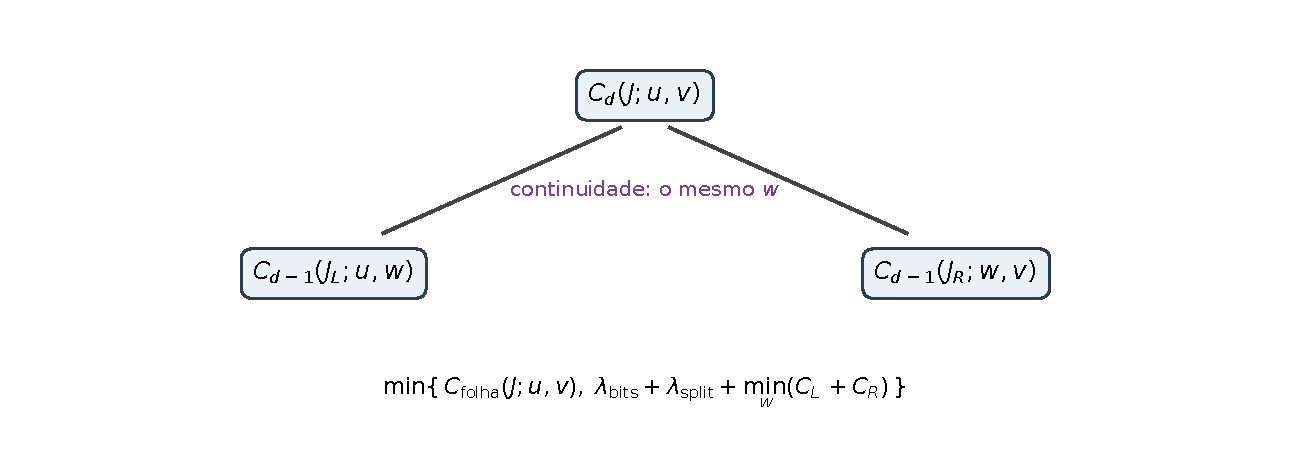
\includegraphics[width=.92\linewidth]{figuras/artigo_2/fig01_estado_fronteira.pdf}
 \caption{O estado registra os dois valores externos; o valor $w$ é
 compartilhado pelos filhos e impõe continuidade. O termo de subdivisão
 inclui o bit do nó interno e a penalidade estrutural.}
 \label{artigo_2:fig:boundary-state}
\end{figure}

% MAPA artigo_2:6.2
\begin{theorem}[correção para árvore fixa]\label{map:artigo_2:6.2}
\label{artigo_2:thm:fixed-correctness}
Para todo nó $J$ de $T$ e todo par de estados $(u,v)$,
\begin{equation}
 C_T(J;u,v)
 =\min_{R\in\Representations_H(T_J;u,v)}
 \cost_{\mathcal Z}(R),
 \label{artigo_2:eq:fixed-correctness}
\end{equation}
com valor $+\infty$ se o conjunto à direita for vazio. Se, em cada mínimo,
for armazenado também o candidato de menor chave \eqref{artigo_2:eq:tie-key}, a
retropropagação reconstrói uma única representação canônica. Em particular,
\begin{equation}
 \min_{u,v\in\Values_{D,H}(K)}C_T(K;u,v)
 =\min_{R\in\Representations_H(T)}\cost_{\mathcal Z}(R).
 \label{artigo_2:eq:fixed-global}
\end{equation}
\end{theorem}

\begin{proof}
Proceda por indução na altura da subárvore. Se $J$ é folha, a
\cref{artigo_2:prop:endpoint-dictionary} mostra que existe exatamente um rótulo com
fronteiras $(u,v)$ quando $(u,v)\in\Pairs_H(J)$, e nenhum nos demais casos.
Seu custo é precisamente \eqref{artigo_2:eq:leaf-cost}, provando
\eqref{artigo_2:eq:fixed-leaf}.

Suponha agora que $J$ tenha filhos. Toda montagem contínua em $T_J$ possui um
único valor $w$ na fronteira compartilhada. Sua restrição aos filhos pertence
a
\[
 \Representations_H(T_{J_L};u,w)
 \quad\text{e}\quad
 \Representations_H(T_{J_R};w,v).
\]
Reciprocamente, quaisquer duas representações desses conjuntos colam-se em
uma representação contínua de $T_J$. Pelo \cref{artigo_2:lem:recursive-stream}, a
colagem acrescenta um bit de nó interno; ela também acrescenta uma
subdivisão. A aditividade da perda e das duas penalidades dá
\eqref{artigo_2:eq:fixed-split}. Aplicar a hipótese de indução aos dois filhos prova
\eqref{artigo_2:eq:fixed-correctness}.

Há um número finito de estados e candidatos. A ordem de
\eqref{artigo_2:eq:tie-key} é total e, pelo \cref{artigo_2:lem:tie-concatenation}, guardar o
menor candidato em cada estado não elimina o minimizador canônico de nenhuma
superárvore. Os apontadores dos valores $w$ e das decisões recuperam esse
candidato. Minimizar também sobre os dois valores externos da raiz prova
\eqref{artigo_2:eq:fixed-global}.
\end{proof}

% MAPA artigo_2:6.3
\begin{algorithm}[rotulação exata de uma árvore fixa]\label{map:artigo_2:6.3}
\label{artigo_2:alg:fixed-tree}
Enumere $\Pairs_H(J)$ em cada folha. Percorra $T$ em pós-ordem. Em cada nó
interno, agrupe os estados do filho direito pelo valor de fronteira esquerdo
$w$ e una apenas pares com o mesmo $w$. Para cada estado externo $(u,v)$,
retenha a menor chave \eqref{artigo_2:eq:tie-key} e um apontador para os dois filhos.
Na raiz, escolha a menor entrada finita e siga os apontadores.
\end{algorithm}

O agrupamento por $w$ não altera a recorrência; ele apenas evita testar pares
de subárvores que violam continuidade de maneira evidente.

\section{Seleção simultânea da árvore e dos átomos}
\label{artigo_2:sec:variable-dp}

Para uma célula $J$ e um inteiro $d\ge0$, seja
\[
 \Representations_{d,H}(J;u,v)
\]
o conjunto das representações contínuas enraizadas em $J$, com profundidade
relativa no máximo $d$, folhas rotuladas por $\Library_H$ e valores externos
$u,v$. Diferentemente da seção anterior, a forma da árvore não é fixada.

A recorrência usa o princípio de otimalidade de \citet{artigo_2-bellman1957}. A
aproximação de curvas por segmentos via programação dinâmica já aparece em
\citet{artigo_2-bellman1961}, com antecedentes para segmentos lineares em
\citet{artigo_2-stone1961} e desenvolvimentos posteriores para aproximação poligonal
ótima em \citet{artigo_2-perezvidal1994}; aqui o estado contém os dois valores de
fronteira e a decisão de manter ou subdividir uma célula diádica.

% MAPA artigo_2:7.1
\begin{definition}[recorrência de Bellman com árvore variável]\label{map:artigo_2:7.1}
\label{artigo_2:def:variable-recurrence}
Para $d=0$, ponha
\begin{equation}
 C_0(J;u,v)=\Phi_H(J;u,v).
 \label{artigo_2:eq:variable-base}
\end{equation}
Para $d\ge1$, se $J_L,J_R$ são os filhos de $J$, defina
\begin{align}
 C_d(J;u,v)
 =\min\Bigl\{&
 \Phi_H(J;u,v),\notag\\
 &\lambda_{\rm bits}+\lambda_{\rm split}
 +\min_{w\in\Values_{D,H}(K)}
 \bigl[C_{d-1}(J_L;u,w)+C_{d-1}(J_R;w,v)\bigr]
 \Bigr\}.
 \label{artigo_2:eq:variable-recurrence}
\end{align}
\end{definition}

O primeiro ramo mantém $J$ como folha; o segundo subdivide, escolhe o valor
racional intermediário e reutiliza os ótimos dos dois filhos. A profundidade
global $D$ é usada somente para fixar um alfabeto comum suficientemente
grande; na chamada em $J$, $d$ é o número de níveis ainda disponíveis.

% MAPA artigo_2:7.2
\begin{theorem}[exatidão, existência e determinismo]\label{map:artigo_2:7.2}
\label{artigo_2:thm:variable-correctness}
Seja $J$ uma célula descendente de $K$ na profundidade relativa $r$. Para todo
$d\le D-r$ e todo $(u,v)\in\Values_{D,H}(K)^2$,
\begin{equation}
 C_d(J;u,v)
 =\min_{R\in\Representations_{d,H}(J;u,v)}
 \cost_{\mathcal Z}(R).
 \label{artigo_2:eq:variable-correctness}
\end{equation}
Consequentemente,
\begin{equation}
 C_{D,H}^{\star}(K)
 :=\min_{u,v\in\Values_{D,H}(K)}C_D(K;u,v)
 =\min_{R\in\Representations_{D,H}^{\Library}(K)}
 \cost_{\mathcal Z}(R).
 \label{artigo_2:eq:variable-global}
\end{equation}
O mínimo é finito quando
$H\ge\max\{2,k_0+1,|m_0|+1\}$. Com o desempate
\eqref{artigo_2:eq:tie-key}, o algoritmo devolve uma única representação, independentemente
da ordem em que estados, átomos ou valores intermediários sejam gerados.
\end{theorem}

\begin{proof}
A prova é por indução em $d$. Para $d=0$, apenas a árvore-folha é permitida,
e \eqref{artigo_2:eq:variable-base} coincide com seu custo ou vale $+\infty$ quando o
par é inadmissível.

Suponha o resultado para $d-1$. Toda representação de profundidade no máximo
$d$ está em exatamente um de dois casos: a raiz é folha; ou a raiz é interna
e possui duas subárvores de profundidade no máximo $d-1$. No segundo caso, a
continuidade produz um único valor compartilhado $w$. Reciprocamente, a
colagem de quaisquer duas subárvores com o mesmo $w$ é admissível. A
decomposição do custo é a mesma do \cref{artigo_2:thm:fixed-correctness}; portanto a
partição exaustiva dos candidatos nos dois casos é exatamente
\eqref{artigo_2:eq:variable-recurrence}. A hipótese de indução completa
\eqref{artigo_2:eq:variable-correctness}.

Minimizar os estados externos na raiz prova \eqref{artigo_2:eq:variable-global}. Sob a
hipótese sobre $H$, o átomo de parâmetros $(k_0,m_0,0,1)$ pertence a
$\Library_H$, logo o catálogo contém ao menos a árvore-folha e o mínimo é
finito. Todos os conjuntos examinados são finitos. A chave
\eqref{artigo_2:eq:tie-key} é total e depende somente do candidato, não da ordem de
geração, o que prova o determinismo.
\end{proof}

% MAPA artigo_2:7.3
\begin{corollary}[compatibilidade com a enumeração de formas]\label{map:artigo_2:7.3}
\label{artigo_2:cor:shape-enumeration}
Se $\Trees_D(K)$ é o conjunto finito de todas as formas de árvore de
profundidade no máximo $D$, então
\begin{equation}
 C_{D,H}^{\star}(K)
 =\min_{T\in\Trees_D(K)}
   \min_{u,v\in\Values_{D,H}(K)}C_T(K;u,v).
 \label{artigo_2:eq:shape-equivalence}
\end{equation}
O mesmo fluxo canônico vence nos dois lados.
\end{corollary}

\begin{proof}
As classes $\Representations_H(T)$, $T\in\Trees_D(K)$, particionam as
representações pela forma da árvore. Aplique os
\cref{artigo_2:thm:fixed-correctness,artigo_2:thm:variable-correctness} e o mesmo desempate
total.
\end{proof}

% MAPA artigo_2:7.4
\begin{algorithm}[seletor exato por programação dinâmica]\label{map:artigo_2:7.4}
\label{artigo_2:alg:variable-tree}
Construa as tabelas em pós-ordem na árvore diádica completa de profundidade
$D$. Inicialize cada estado com o candidato folha, quando admissível. Una as
tabelas dos filhos pelo valor intermediário $w$, acrescente o marcador e a
penalidade de subdivisão e substitua a entrada somente quando a chave completa
diminuir. A tabela da raiz e os apontadores guardados fornecem o ótimo global
e sua representação.
\end{algorithm}

\section{Orçamentos rígidos e erro uniforme}
\label{artigo_2:sec:hard-budgets}

Além do funcional penalizado, um orçamento explícito de folhas pode ser
incorporado ao estado sem alterar o princípio de otimalidade.

\subsection{Número exato de folhas}

Para $1\le n\le2^d$, defina $C_{d,n}(J;u,v)$ como o menor valor de
\eqref{artigo_2:eq:additive-objective} entre representações com exatamente $n$ folhas.
A recorrência é
\begin{align}
 C_{0,1}(J;u,v)&=\Phi_H(J;u,v),\label{artigo_2:eq:budget-base}\\
 C_{0,n}(J;u,v)&=+\infty,\qquad n>1,\notag\\
 C_{d,1}(J;u,v)&=\Phi_H(J;u,v),\qquad d\ge1,\label{artigo_2:eq:budget-one}\\
 C_{d,n}(J;u,v)&=\lambda_{\rm bits}+\lambda_{\rm split}\notag\\
 &\quad+\min_{\substack{n_L+n_R=n\\n_L,n_R\ge1}}
 \min_{w\in\Values_{D,H}(K)}
 \{C_{d-1,n_L}(J_L;u,w)+C_{d-1,n_R}(J_R;w,v)\},
 \quad n\ge2.
 \label{artigo_2:eq:budget-recurrence}
\end{align}

% MAPA artigo_2:8.1
\begin{theorem}[correção sob orçamento de folhas]\label{map:artigo_2:8.1}
\label{artigo_2:thm:leaf-budget}
As recorrências \eqref{artigo_2:eq:budget-base}--\eqref{artigo_2:eq:budget-recurrence}
calculam exatamente o menor custo entre representações de profundidade no
máximo $d$, altura no máximo $H$, fronteiras $(u,v)$ e exatamente $n$
folhas. Em particular, o ótimo com no máximo $N$ folhas é
\begin{equation}
 \min_{\substack{1\le n\le\min\{N,2^D\}\\
                  u,v\in\Values_{D,H}(K)}}
 C_{D,n}(K;u,v).
 \label{artigo_2:eq:at-most-N}
\end{equation}
\end{theorem}

\begin{proof}
A indução em $d$ é idêntica à do
\cref{artigo_2:thm:variable-correctness}, com uma coordenada adicional. Uma
representação com uma folha usa o primeiro ramo. Se possui $n\ge2$ folhas,
sua raiz é interna e as quantidades positivas de folhas dos filhos satisfazem
$n_L+n_R=n$. Reciprocamente, toda escolha listada em
\eqref{artigo_2:eq:budget-recurrence} cola duas representações com exatamente $n$
folhas. A união sobre $1\le n\le N$ prova \eqref{artigo_2:eq:at-most-N}.
\end{proof}

\subsection{Recorrência de gargalo para a norma uniforme}

Seja agora $f\in C(K)$ e suponha disponível, para cada par admissível, o erro
local exato
\begin{equation}
 e_f(J;u,v)=\|f-\ell_{J;u,v}\|_{\infty,J}.
 \label{artigo_2:eq:local-uniform-error}
\end{equation}
Quando o par é inadmissível, ponha $e_f=+\infty$. Não se supõe que esse oráculo
exista para toda apresentação de uma função contínua; para polinômios e
famílias elementares ele pode ser produzido por cálculo simbólico ou por
aritmética intervalar certificada.

Defina $B_{d,n}(J;u,v)$ substituindo soma de perdas pelo máximo entre folhas:
\begin{align}
 B_{0,1}(J;u,v)&=e_f(J;u,v),\label{artigo_2:eq:bottleneck-base}\\
 B_{0,n}(J;u,v)&=+\infty,\qquad n>1,\notag\\
 B_{d,1}(J;u,v)&=e_f(J;u,v),\label{artigo_2:eq:bottleneck-one}\\
 B_{d,n}(J;u,v)
 &=\min_{\substack{n_L+n_R=n\\n_L,n_R\ge1}}
 \min_{w\in\Values_{D,H}(K)}
 \max\{B_{d-1,n_L}(J_L;u,w),
       B_{d-1,n_R}(J_R;w,v)\}.
 \label{artigo_2:eq:bottleneck-recurrence}
\end{align}

Seja
\begin{equation}
 E_{N,H,D}^{\rm tree}(f)_\infty
 =\min\{\|f-\Eval(R)\|_{\infty,K}:
 R\in\Representations_{D,H}^{\Library}(K),\
 |\Lambda(R)|\le N\}.
 \label{artigo_2:eq:truncated-tree-error}
\end{equation}

% MAPA artigo_2:8.2
\begin{theorem}[cálculo exato do melhor erro truncado]\label{map:artigo_2:8.2}
\label{artigo_2:thm:bottleneck}
Sob o oráculo \eqref{artigo_2:eq:local-uniform-error},
\begin{equation}
 E_{N,H,D}^{\rm tree}(f)_\infty
 =\min_{\substack{1\le n\le\min\{N,2^D\}\\
                  u,v\in\Values_{D,H}(K)}}
 B_{D,n}(K;u,v).
 \label{artigo_2:eq:bottleneck-optimum}
\end{equation}
Se
\begin{equation}
 D\ge \max\{0,H-k_0-1\},
 \label{artigo_2:eq:depth-inactive}
\end{equation}
a restrição de profundidade já é inativa: nenhum átomo de $\Library_H$
apoiado em descendente de $K$ pode ocorrer abaixo desse nível.
\end{theorem}

\begin{proof}
Em uma montagem contínua, o erro uniforme global é o máximo dos erros nas
folhas. A mesma partição em raiz-folha ou raiz-interna usada no
\cref{artigo_2:thm:leaf-budget} produz
\eqref{artigo_2:eq:bottleneck-recurrence}, agora com o operador máximo na colagem.
A indução em $d$ prova que $B_{d,n}$ é o melhor gargalo com o estado e a
quantidade de folhas fixados. Minimizar essas coordenadas dá
\eqref{artigo_2:eq:bottleneck-optimum}.

Uma folha na profundidade relativa $r$ tem escala $k_0+r$. Pela altura
\eqref{artigo_2:eq:inherited-height}, sua admissibilidade exige
$k_0+r+1\le H$. Portanto $r\le H-k_0-1$, o que prova a última afirmação.
\end{proof}

% MAPA artigo_2:8.3
\begin{remark}[interação entre profundidade e translação]\label{map:artigo_2:8.3}
\label{artigo_2:rem:depth-vs-translation}
A condição \eqref{artigo_2:eq:depth-inactive} satura o ganho obtido pelo aumento de $D$
além de $H-k_0-1$. A admissibilidade de cada célula também depende de sua
posição.
Para $m_0\ge0$, a \cref{artigo_2:prop:translation-obstruction} mostra que o refinamento
uniforme completo exige também
$r\le\log_2\bigl(H/(m_0+1)\bigr)$. Quando esse segundo limiar é o menor, o
catálogo se torna espacialmente assimétrico antes de a escala se esgotar. Ao ler
\eqref{artigo_2:eq:bottleneck-optimum} para um dado $(N,H,D)$, portanto, o orçamento de
folhas $N$ compete com uma família de árvores que já está truncada pela
translação, não apenas pela profundidade.
\end{remark}

% MAPA artigo_2:8.4
\begin{corollary}[convergência para funções contínuas]\label{map:artigo_2:8.4}
\label{artigo_2:cor:uniform-convergence}
Para todo $f\in C(K)$,
\begin{equation}
 \inf_{N,H,D}E_{N,H,D}^{\rm tree}(f)_\infty=0.
 \label{artigo_2:eq:uniform-convergence}
\end{equation}
Mais precisamente, ao longo de qualquer sequência de triplas $(N,H,D)$ que
seja componente a componente não decrescente e cofinal, os erros convergem a
zero.
\end{corollary}

\begin{proof}
Os catálogos são aninhados em cada orçamento, logo os erros não crescem. O
teorema de densidade da \cref{artigo_2:sec:assemblies} afirma que, dado $\varepsilon>0$,
existe uma montagem contínua finita de átomos com erro menor que
$\varepsilon$. Essa representação possui números finitos de folhas,
profundidade e altura; portanto pertence a algum catálogo da união. Assim, o
ínfimo em \eqref{artigo_2:eq:uniform-convergence} é zero, e a monotonicidade prova a
convergência cofinal.
\end{proof}

\section{Complexidade, truncagem e estabilidade}
\label{artigo_2:sec:complexity-dp}

\subsection{Contagem de operações}

Escreva
\[
 M=|\Values_{D,H}(K)|,\qquad S_D=2^{D+1}-1.
\]
As cotas abaixo usam o modelo de custo unitário para operações e comparações
no corpo ordenado dos custos. O tamanho dos operandos racionais será discutido
separadamente. O custo do terceiro componente da chave \eqref{artigo_2:eq:tie-key}, o
\emph{fluxo binário completo}, é contado em bits. Comparar duas
chaves que empatam nas duas primeiras componentes custa
$O(L)$, onde
\begin{equation}
 L=\max_R|\ser_{\rm rec}(R)|
 \le S_D\bigl(2\lfloor\log_2|\Library_H|\rfloor+2\bigr)
 \label{artigo_2:eq:stream-length}
\end{equation}
é o comprimento máximo de fluxo no catálogo. Todas as cotas desta seção contam
comparações de chave e construção/concatenação de fluxos como unitárias;
multiplicá-las por $L$ dá uma cota superior correspondente no modelo em que
comparar ou copiar um bit tem custo unitário.
Pela mesma razão, as cotas de memória contam \emph{entradas} da tabela, e cada
entrada que armazena um fluxo ocupa até $L$ bits. Uma implementação que
guarde apenas ponteiros de reconstrução e recomponha o fluxo sob demanda
troca esse fator de memória por trabalho adicional na comparação.

% MAPA artigo_2:9.1
\begin{theorem}[complexidade em número de estados]\label{map:artigo_2:9.1}
\label{artigo_2:thm:state-complexity}
Suponha os custos de folha pré-computados. Uma implementação densa do
\cref{artigo_2:alg:variable-tree} usa
\begin{equation}
 O(S_DM^3)
 \label{artigo_2:eq:dense-time}
\end{equation}
operações e
\begin{equation}
 O(S_DM^2)
 \label{artigo_2:eq:dense-memory}
\end{equation}
entradas de memória quando preserva todos os apontadores de reconstrução.
A versão com orçamento de até $N$ folhas usa
\begin{equation}
 O(S_DN^2M^3)
 \label{artigo_2:eq:budget-time}
\end{equation}
operações e $O(S_DNM^2)$ entradas. Se cada custo local
\eqref{artigo_2:eq:local-loss} for calculado diretamente sobre $P$ observações, a
inicialização densa acrescenta $O(S_DPM^2)$ operações.
\end{theorem}

\begin{proof}
Cada nó tem no máximo $M^2$ estados externos $(u,v)$. Em um nó interno, a
recorrência testa no máximo $M$ valores intermediários $w$ por estado, logo
$O(M^3)$ operações. Há no máximo $S_D$ nós. Armazenar um custo e um apontador
por estado dá \eqref{artigo_2:eq:dense-memory}.

Com o número de folhas no estado, há $N$ camadas de custo. Somando, para todos
$n\le N$, as decomposições positivas $n_L+n_R=n$, obtêm-se $O(N^2)$ pares de
orçamentos por tripla $(u,w,v)$. Isso prova \eqref{artigo_2:eq:budget-time} e a cota de
memória. A última afirmação vem de somar até $P$ termos em cada custo local.
\end{proof}

% MAPA artigo_2:9.2
\begin{remark}[tabelas esparsas]\label{map:artigo_2:9.2}
\label{artigo_2:rem:sparse}
As cotas são deliberadamente densas. O algoritmo distribuído armazena apenas
pares realizáveis e agrupa o filho direito por $w$. Seu trabalho em um nó é
proporcional ao tamanho da junção
\[
 \#\{((u,w),(w,v)):\text{os dois estados estão presentes}\},
\]
que pode ser muito menor que $M^3$. Essa melhora depende da instância e não
altera a cota de pior caso.

Na instância principal da \cref{artigo_2:sec:numerical}, com
$(D,H)=(3,4)$, o alfabeto efetivo tem $M=475$ elementos, contra
$2S_Dq_H(q_H-1)=15\,180$ pela primeira cota de
\eqref{artigo_2:eq:value-alphabet-bound} e $36H^6=147\,456$ pela segunda; e a tabela da
raiz contém $3383$ estados realizáveis, contra $M^2=225\,625$ posições
densas, isto é, uma ocupação de $1{,}5\%$. Nas instâncias examinadas, a
estrutura esparsa reduz substancialmente o trabalho em relação à cota densa de
pior caso.
\end{remark}

\subsection{Modelo de custo e complexidade de bits}

Pelo \cref{artigo_2:lem:value-alphabet},
\[
 M\le36H^6,
\]
e portanto \eqref{artigo_2:eq:dense-time} fornece, de modo bruto,
\begin{equation}
 O(S_DH^{18})
 \label{artigo_2:eq:height-worst}
\end{equation}
operações de custo unitário. A expressão é polinomial no valor numérico de
$H$, cujo comprimento binário é $O(\log H)$, e
$S_D=2^{D+1}-1$. Trata-se, portanto, de uma cota pseudo-polinomial nos
orçamentos codificados em binário.

Para fechar também esse segundo nível, defina, para $r=p/q$ reduzido, $q>0$,
\begin{equation}
 \operatorname{bl}(r)
 :=1+\left\lceil\log_2(|p|+1)\right\rceil
    +\left\lceil\log_2(q+1)\right\rceil .
 \label{artigo_2:eq:rational-bit-length}
\end{equation}
Seja $B_{\mathcal Z}$ o maior comprimento \eqref{artigo_2:eq:rational-bit-length}
entre abscissas, respostas, pesos e penalidades racionais da instância. Denote
por $\mathsf M_{\mathbb Z}(b)$ uma cota para multiplicar inteiros de $b$ bits,
e recorde o limite $L$ de \eqref{artigo_2:eq:stream-length}.

% MAPA artigo_2:9.3
\begin{theorem}[cota grosseira de complexidade de bits]\label{map:artigo_2:9.3}
\label{artigo_2:thm:bit-complexity}
Todos os custos racionais que aparecem na recorrência possuem numeradores e
denominadores de comprimento no máximo
\begin{equation}
 B_{\rm cost}
 =O\!\left(
 P\bigl(B_{\mathcal Z}+D+|k_0|+\log(2H)\bigr)
 +B_{\mathcal Z}+D+\log(2L)
 \right).
 \label{artigo_2:eq:cost-bit-growth}
\end{equation}
Consequentemente, a versão densa sem orçamento de folhas pode ser executada em
\begin{equation}
 O\!\left(
 (S_DM^3+S_DPM^2)
 \bigl[\mathsf M_{\mathbb Z}(B_{\rm cost})
       \log(2B_{\rm cost})+L\bigr]
 \right)
 \label{artigo_2:eq:dense-bit-time}
\end{equation}
operações de bit e
\begin{equation}
 O\!\left(S_DM^2(B_{\rm cost}+L)\right)
 \label{artigo_2:eq:dense-bit-memory}
\end{equation}
bits de memória quando todos os estados e fluxos são armazenados. Na versão
com até $N$ folhas, substituem-se $S_DM^3$ e $S_DM^2$ por
$S_DN^2M^3$ e $S_DNM^2$, respectivamente. Com multiplicação escolar,
$\mathsf M_{\mathbb Z}(b)=O(b^2)$.
\end{theorem}

\begin{proof}
Um átomo admissível tem $\operatorname{bl}(y_0),
\operatorname{bl}(s)=O(\log(2H))$. Em uma célula descendente de profundidade
no máximo $D$, escrever o centro ou um extremo como racional expande o fator
diádico em no máximo $D+|k_0|+O(1)$ bits. Portanto a avaliação afim em uma
abscissa da amostra tem comprimento
\[
 O(B_{\mathcal Z}+D+|k_0|+\log(2H)).
\]
Subtrair a resposta, elevar ao quadrado e multiplicar pelo peso apenas altera
a constante dessa cota. Na soma ingênua de $P$ frações, pode-se tomar como
denominador o produto dos denominadores; logo numerador e denominador têm
comprimento no máximo $P$ vezes o maior comprimento de uma parcela. Os termos
de penalização acrescentam $O(B_{\mathcal Z}+D+\log(2L))$ bits. Isso prova
\eqref{artigo_2:eq:cost-bit-growth}; cancelamentos por máximo divisor comum só podem
reduzir os operandos.

Uma soma, comparação ou redução de frações com operandos de comprimento
$B_{\rm cost}$ custa
$O(\mathsf M_{\mathbb Z}(B_{\rm cost})\log(2B_{\rm cost}))$ operações de bit
por algoritmos inteiros usuais. Quando custos e número de folhas empatam, a
comparação shortlex lê no máximo $L$ bits. Multiplicar esse custo pelo número
de transições e inicializações do \cref{artigo_2:thm:state-complexity} dá
\eqref{artigo_2:eq:dense-bit-time}. Cada estado guarda um custo, um fluxo ou apontador
de reconstrução e índices de $O(\log(S_DM))$ bits, absorvidos pela cota exibida;
isso prova \eqref{artigo_2:eq:dense-bit-memory}. O argumento com a coordenada de
orçamento é idêntico.
\end{proof}

A cota é propositalmente conservadora: ela não explora cancelamentos nem
denominadores compartilhados. Ainda assim, fecha o modelo de Turing e torna
explícito o ponto essencial. Como $M\le36H^6$ e $S_D=2^{D+1}-1$, a
dependência continua pseudo-polinomial nos valores numéricos de $H$ e $2^D$,
mesmo após contabilizar o crescimento dos racionais.

\subsection{Valores sob truncagem}

Seja
\[
 \Representations_{\infty}^{\Library}(K)
 =\bigcup_{D,H}\Representations_{D,H}^{\Library}(K)
\]
o conjunto de todas as representações finitas enraizadas em $K$.

% MAPA artigo_2:9.4
\begin{proposition}[convergência dos mínimos penalizados]\label{map:artigo_2:9.4}
\label{artigo_2:prop:truncation-convergence}
Os valores $C_{D,H}^{\star}(K)$ de \eqref{artigo_2:eq:variable-global} são não
crescentes separadamente em $D$ e $H$, e
\begin{equation}
 \inf_{D,H}C_{D,H}^{\star}(K)
 =\inf_{R\in\Representations_{\infty}^{\Library}(K)}
   \cost_{\mathcal Z}(R).
 \label{artigo_2:eq:penalized-limit}
\end{equation}
Ao longo de qualquer sequência componente a componente não decrescente e
cofinal em $(D,H)$, os valores convergem ao lado direito.

Se o ínfimo em \eqref{artigo_2:eq:penalized-limit} é atingido, o minimizador global de
menor chave \eqref{artigo_2:eq:tie-key} pertence a algum catálogo finito; a partir de
uma truncagem que o contenha, o seletor canônico estabiliza.
\end{proposition}

\begin{proof}
Aumentar $D$ ou $H$ preserva toda representação já admissível, logo os
mínimos não crescem. A união dos domínios dos mínimos é exatamente
$\Representations_{\infty}^{\Library}(K)$, o que prova
\eqref{artigo_2:eq:penalized-limit}. Uma sequência cofinal eventualmente contém cada
representação finita; a monotonicidade conclui a convergência.

Se há minimizadores globais, seus comprimentos de fluxo formam um subconjunto
não vazio de $\Nzero$ e possuem mínimo. Entre as finitíssimas palavras desse
comprimento existe uma menor lexicograficamente. A representação
correspondente tem profundidade e altura finitas. Depois que ela entra no
catálogo, nenhum candidato posterior pode melhorar o custo ou a chave.
\end{proof}

\subsection{Um limite de estabilidade}

% MAPA artigo_2:9.5
\begin{proposition}[um seletor exato pode ser descontínuo]\label{map:artigo_2:9.5}
\label{artigo_2:prop:instability}
Considere, em $K=[0,1]$, o subcatálogo formado pelos dois átomos
\[
 g_+(x)=x,\qquad g_-(x)=-x,
\]
ambos de altura $2$. Para uma única observação $(x,z)=(1,z)$, custo igual à
perda quadrática e qualquer desempate determinístico, o mapa que envia $z$ ao
átomo selecionado é descontínuo em $z=0$ na norma uniforme.
\end{proposition}

\begin{proof}
Os custos são
\[
 \cost_z(g_+)=(z-1)^2,\qquad
 \cost_z(g_-)=(z+1)^2.
\]
Logo $g_+$ é o único minimizador para $z>0$, $g_-$ é o único minimizador para
$z<0$ e há empate em $z=0$. Qualquer regra escolhe um deles no empate, mas a
sequência que se aproxima por dados do lado oposto seleciona sempre o outro.
Como
\[
 \|g_+-g_-\|_{\infty,[0,1]}=2,
\]
não há continuidade.
\end{proof}

O exemplo separa exatidão de continuidade do seletor. Hipóteses de margem
entre custos produzem regiões de seleção localmente constante; nos empates,
uma saída a valores conjuntos preserva semicontinuidade. Essa distinção entre
existência, estabilidade e não unicidade também aparece na análise de problemas
de treinamento por perda quadrática em esquemas não lineares
\citep{artigo_1-christof2021}.

\section{Validação computacional exata}
\label{artigo_2:sec:numerical}

\subsection{Implementação}

O script
\path{verificacao/seletor_dinamico_exato.py}
implementa os \cref{artigo_2:alg:fixed-tree,artigo_2:alg:variable-tree}. O domínio numérico é
\texttt{Fraction}. As tabelas são dicionários esparsos indexados
por pares de \texttt{Fraction}; a junção dos filhos usa igualdade racional
exata no valor $w$. Perdas, penalidades, comparações de objetivo, alturas,
endereços $\Gamma^\sharp$ e desempates não usam ponto flutuante.
\texttt{NumPy} e \texttt{Matplotlib} aparecem somente depois da seleção, para
desenhar as figuras.

Cada execução verifica:
\begin{enumerate}[label=(\alph*),leftmargin=2em]
 \item a continuidade de todas as fronteiras da montagem vencedora;
 \item a altura de cada folha;
 \item a igualdade entre o ótimo da recorrência variável e o mínimo obtido ao
 enumerar separadamente todas as formas e resolver cada árvore fixa;
 \item a coincidência com uma enumeração direta de representações na
 instância mínima descrita abaixo;
 \item que uma derivação separada de $\mathcal Q_H$, dos pares de extremos
 e das perdas locais coincide com as rotinas usadas pela PD;
 \item as recorrências com número exato de folhas e de gargalo contra
 enumeração sem poda;
 \item a robustez da comparação num orçamento sem células eliminadas;
 \item que o valor exato não excede os valores das três referências.
\end{enumerate}

O verificador de (d) é independente da \emph{recorrência}, mas reutiliza o
catálogo local e a função de perda. Por isso (e) constitui uma segunda camada:
ela enumera $\mathcal Q_H$ diretamente pelas frações reduzidas, forma os pares
de extremos a partir de $(y_0,s)$ sem chamar o dicionário da PD e recompõe
\eqref{artigo_2:eq:local-loss} pela fórmula afim nos pontos observados. As duas
comparações possuem, assim, implementações independentes do dicionário e da
perda. O teste de erro uniforme em (f) usa $f\equiv0$, caso em que
$e_f(J;u,v)=\max\{|u|,|v|\}$ é calculado exatamente.

\subsection{Auditoria por enumeração direta}

Na instância de auditoria, tomam-se $(D,H)=(1,2)$, as cinco observações
racionais $x_i\in\{0,\tfrac14,\tfrac12,\tfrac34,1\}$ do alvo $2|x-1/2|$ e as
penalidades $\lambda_{\rm bits}=\tfrac1{200}$,
$\lambda_{\rm split}=\tfrac1{50}$. Há $42$ átomos admissíveis na
raiz. O verificador examina diretamente os $42$ candidatos de uma folha e
todos os $42^2=1764$ pares de átomos dos filhos, descartando os $1704$ pares
que não coincidem em $x=1/2$. Restam $60$ subdivisões contínuas, ou $102$
representações ao contar também as folhas. O custo e o fluxo vencedores
coincidem bit a bit com a programação dinâmica.

Nessa instância, como na instância principal, o minimizador de custo é único,
de modo que ela não chega a exercitar o desempate \eqref{artigo_2:eq:tie-key}. O script
inclui por isso três cenários dedicados, nos quais o vencedor da recorrência é
confrontado com a minimização exaustiva da chave completa sobre todas as
representações contínuas, enumeradas \emph{sem} poda por estado:
\begin{enumerate}[label=(\alph*),leftmargin=2em]
 \item com dados e penalidades nulos e $(D,H)=(1,2)$, todas as $102$
 representações têm custo zero e a seleção é decidida pelo comprimento do
 fluxo;
 \item o mesmo com $(D,H)=(2,3)$, em que as $1370$ representações contínuas
 empatam em custo, o que exercita dois níveis de concatenação;
 \item com dados identicamente nulos e $(D,H)=(2,3)$, dois candidatos empatam
 simultaneamente em custo e em comprimento, e a seleção é decidida pela ordem
 lexicográfica do fluxo.
\end{enumerate}
Nos três casos a recorrência devolve exatamente o mesmo fluxo que a
minimização exaustiva, o que verifica a compatibilidade de \eqref{artigo_2:eq:tie-key}
com a concatenação afirmada no \cref{artigo_2:thm:fixed-correctness}.

Para testar a \cref{artigo_2:sec:hard-budgets}, o script enumera sem poda todas as
$1370$ representações contínuas de $(D,H)=(2,3)$. Para cada número viável de
folhas e cada par de estados externos, compara tanto o melhor custo aditivo
$C_{d,n}$ quanto o melhor gargalo $B_{d,n}$ com a enumeração completa. Também
compara, para cada $N\in\{1,2,3,4\}$, o ótimo com no máximo $N$ folhas. Todas
as igualdades são verificadas em aritmética racional exata.

\begin{table}[t]
 \centering
 \caption{Verificações executáveis das duas instâncias.}
 \label{artigo_2:tab:dp-audit}
 \small
 \begin{tabularx}{\linewidth}{@{}Xr@{}}
\toprule
Verificação & resultado \\
\midrule
Dicionário/perdas derivados das definições & true \\
Enumeração direta $(D,H)=(1,2)$ & true \\
Pares de subárvores examinados diretamente & 1764 \\
Formas de árvore enumeradas na instância principal & 26 \\
Formas de árvore com catálogo não vazio & 11 \\
Células da árvore completa sem átomo admissível & 4 \\
DP variável $=$ mínimo sobre formas fixas & true \\
Empates de custo máximos resolvidos pela chave & 1370 \\
DP $=$ mínimo exaustivo sob empate & true \\
Fórmula geométrica (1350 casos) & true \\
Orçamento de folhas $=$ enumeração exaustiva & true \\
Gargalo uniforme $=$ enumeração exaustiva & true \\
Ótimo exato não pior que as três referências & true \\
\bottomrule
\end{tabularx}

\end{table}

As contagens e os fluxos da \cref{artigo_2:tab:dp-audit} coincidem com a enumeração
exaustiva independente em todas as instâncias indicadas, inclusive para a
recorrência de gargalo do \cref{artigo_2:thm:bottleneck}.

\subsection{Instância de regressão e rotas de controle}

A instância seguinte verifica a correção do seletor. As três rotas auxiliares fornecem candidatos admissíveis sob o mesmo funcional; seus custos são comparados ao mínimo exato do catálogo. A comparação se restringe a essa instância sintética.

A instância principal usa $K=[0,1]$, $(D,H)=(3,4)$ e as $17$ observações
diádicas $x_i=i/16$ do alvo racional
\begin{equation}
 f(x)=\frac{1}{1+16(x-\tfrac14)^2},
 \label{artigo_2:eq:experiment-target}
\end{equation}
com respostas $z_i=f(x_i)$ e pesos unitários $\omega_i=1$. As penalidades são
\[
 \lambda_{\rm bits}=\frac1{500},
 \qquad
 \lambda_{\rm split}=\frac1{100}.
\]
Há $23$ valores racionais e $22$ inclinações não nulas de altura no máximo
$4$, isto é, $506$ átomos por célula geometricamente admissível. A árvore
completa possui $15$ células, das quais $11$ são admissíveis: pela
\cref{artigo_2:prop:translation-obstruction}, as quatro células de profundidade $3$ que
cobrem $[\tfrac12,1]$ têm $m\in\{4,5,6,7\}$ e nenhum átomo de altura no
máximo $4$. Consequentemente, das $26$ formas de árvore de profundidade no
máximo $3$, apenas $11$ admitem alguma rotulação contínua; as $15$ restantes
--- todas as que subdividem a metade direita até a profundidade $3$ --- têm
catálogo vazio. As $26$ formas são enumeradas para auditoria, e o mínimo sobre
as viáveis coincide com a recorrência variável. A tabela esparsa da raiz
contém $3383$ estados realizáveis.

Essa assimetria deve ser mantida em vista ao ler a tabela: nesta instância a
metade esquerda do domínio é refinável até a profundidade $3$ e a metade
direita apenas até a profundidade $2$.

As rotas de controle são definidas sob o mesmo funcional:
\begin{itemize}[leftmargin=1.7em]
 \item \emph{malha uniforme}: escolhe o melhor entre as árvores completas de
 profundidades $0,1,2,3$, rotulando cada uma exatamente. Nesta instância a
 profundidade $3$ é \emph{inviável} --- sua metade direita não admite
 rotulação alguma ---, de modo que a escolha se dá de fato entre as
 profundidades $0$, $1$ e $2$, com objetivos $0{,}565803$, $0{,}572135$ e
 $0{,}376159$; vence a profundidade $2$, com quatro folhas;
 \item \emph{adaptativo certificado}: subdivide quando
 $M(J)|J|^2/8>\varepsilon_I$ e depois rotula a árvore exatamente; para
 \eqref{artigo_2:eq:experiment-target},
 \[
 f''(x)=
 \frac{32\bigl(48(x-\tfrac14)^2-1\bigr)}
      {\bigl(1+16(x-\tfrac14)^2\bigr)^3},
 \]
 e o máximo local é calculado racionalmente nos pontos críticos. O programa
 percorre $\varepsilon_I\in\{2^{-1},\dots,2^{-10}\}$ e retém o melhor
 resultado sob o mesmo objetivo da regressão; o caso retido é
 $\varepsilon_I=\tfrac12$. Registre-se que esse ajuste favorece a referência,
 e que apertar o certificado não ajuda: $\varepsilon_I\in\{2^{-3},2^{-4}\}$
 produz seis folhas e objetivo $0{,}571837$, e $\varepsilon_I\le2^{-5}$ exige
 uma árvore fora do catálogo;
 \item \emph{guloso}: começa na raiz, testa cada subdivisão de uma única folha,
 reotimiza exatamente todos os rótulos da árvore candidata e aceita apenas
 uma redução imediata do objetivo.
\end{itemize}

\begin{table}[t]
 \centering
 \caption{Regressão sob o mesmo custo racional. Os decimais são
 apresentações dos valores exatos registrados em
 \texttt{verificacao/resultados.json}.}
 \label{artigo_2:tab:selector-comparison}
 \small
 \begin{tabular}{lrrrr}
\toprule
Método & folhas & erro quadrático & bits & objetivo \\
\midrule
Ótimo exato & 3 & 0{,}041497 & 84 & 0{,}229497 \\
Malha uniforme & 4 & 0{,}116159 & 115 & 0{,}376159 \\
Adaptativo certificado & 3 & 0{,}041497 & 84 & 0{,}229497 \\
Heurística gulosa & 1 & 0{,}517803 & 24 & 0{,}565803 \\
\bottomrule
\end{tabular}

\end{table}

O ótimo exato possui três folhas:
\[
 [0,\tfrac14],\qquad[\tfrac14,\tfrac12],\qquad[\tfrac12,1],
\]
com valores nodais
\[
 \frac12,\quad1,\quad\frac12,\quad0.
\]
Suas inclinações são $2,-2,-1$ e sua altura máxima é $4$. O refinamento
certificado com $\varepsilon_I=\tfrac12$ coincide com essa árvore nesta
instância. 
A melhor malha uniforme viável usa quatro folhas e tem
custo maior. A heurística gulosa permanece na raiz: a única subdivisão isolada
disponível eleva o objetivo de $0{,}565803$ para $0{,}572135$, embora duas
subdivisões coordenadas o reduzam para $0{,}229497$. O exemplo torna
visível a razão algorítmica para preservar estados e subproblemas em vez de
tomar apenas decisões locais.

\begin{figure}[t]
 \centering
 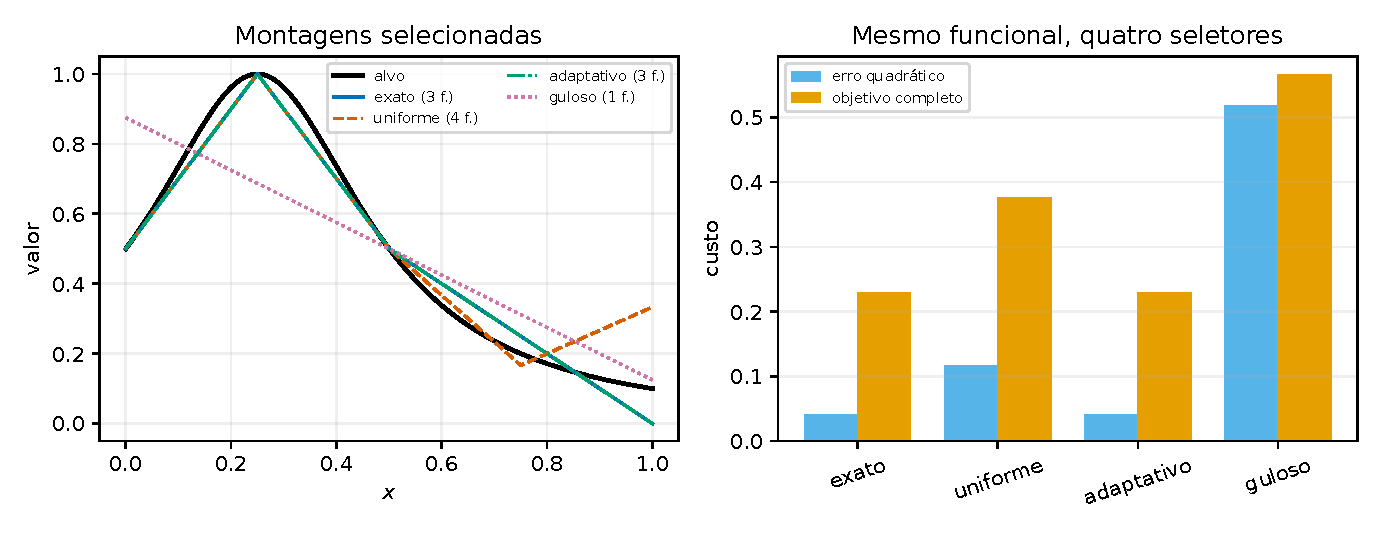
\includegraphics[width=\linewidth]{figuras/artigo_2/fig02_comparacao_seletores.pdf}
 \caption{À esquerda, o alvo e as quatro montagens. À direita, erro quadrático e objetivo completo. As decisões usam racionais exatos; o desenho usa ponto flutuante.}
 \label{artigo_2:fig:selector-comparison}
\end{figure}

As montagens da regressão aparecem na
\cref{artigo_2:fig:selector-comparison}; os valores exatos correspondentes estão na
\cref{artigo_2:tab:selector-comparison}.

\subsection{Propriedades verificadas}

A regressão confirma o mínimo do catálogo e o reaproveitamento de subproblemas. Na instância examinada, o candidato guloso permanece na raiz, enquanto duas subdivisões coordenadas reduzem o custo.

\subsection{Robustez sob truncagem do catálogo}
\label{artigo_2:sec:robustness}

Na instância $(D,H)=(3,4)$, a geometria do catálogo admite $11$ árvores e
elimina a malha uniforme mais fina. Para isolar esse efeito, tome
$(D,H)=(2,4)$, que satisfaz as duas
condições da \cref{artigo_2:prop:translation-obstruction} --- $k_0+D+1\le H$ e
$2^D(m_0+1)\le H$ ---, de modo que a árvore completa é integralmente
admissível: nenhuma célula é vazia e as cinco formas de profundidade no máximo
$2$ são viáveis. Com o mesmo alvo e as mesmas penalidades, as quatro rotas
produzem
\[
 0{,}229497,\quad 0{,}376159,\quad 0{,}229497,\quad 0{,}565803,
\]
com $3$, $4$, $3$ e $1$ folhas: exatamente os valores da
\cref{artigo_2:tab:selector-comparison}. O ótimo exato coincide, inclusive no fluxo
binário, com o da instância truncada --- pois suas três
folhas $[0,\tfrac14]$, $[\tfrac14,\tfrac12]$, $[\tfrac12,1]$ nunca descem
abaixo da profundidade $2$.

A truncagem por translação exclui corretamente a malha uniforme de
profundidade $3$, enquanto preserva o ótimo e seu fluxo binário. Em ambas as
instâncias, a rota gulosa implementada permanece presa na raiz; os valores indicados são os dessas duas instâncias.

\section{Erro interpolatório ótimo em árvores estritamente diádicas}
\label{artigo_2:sec:dyadic-asymptotic}

Fixe primeiro o objeto cuja constante será determinada. Para uma célula
diádica $J=[a,b]$ e $f\in C(J)$, denote por $P_Jf$ a reta que interpola
$f(a)$ e $f(b)$ e ponha
\begin{equation}
 e_f(J)=\|f-P_Jf\|_{\infty,J}.
 \label{artigo_2:eq:local-interpolation-error}
\end{equation}
Se $\Lambda$ é o conjunto de folhas de uma árvore diádica finita com raiz
$K$, as retas $P_Jf$, $J\in\Lambda$, concordam nos nós compartilhados e
definem o interpolante contínuo $P_\Lambda f$. Defina
\begin{equation}
 E_N^{\rm dia}(f)_\infty
 =\min_{\substack{\Lambda\text{ árvore diádica}\\ |\Lambda|\le N}}
   \|f-P_\Lambda f\|_{\infty,K}
 =\min_{\substack{\Lambda\text{ árvore diádica}\\ |\Lambda|\le N}}
   \max_{J\in\Lambda}e_f(J).
 \label{artigo_2:eq:optimal-dyadic-interpolation}
\end{equation}
O mínimo existe: há apenas um número finito de árvores binárias ordenadas e
cheias com no máximo $N$ folhas, e uma árvore com $n$ folhas tem profundidade
no máximo $n-1$.

O sobrescrito ``dia'' distingue \eqref{artigo_2:eq:optimal-dyadic-interpolation} do
erro truncado \eqref{artigo_2:eq:truncated-tree-error}. O primeiro otimiza a
\emph{árvore} e fixa em cada folha a reta interpoladora real; o segundo
otimiza simultaneamente árvore e rótulos racionais de altura no máximo $H$.
As constantes abaixo pertencem ao primeiro problema.
Elas serão comparadas com a referência de nós livres apresentada nas preliminares; a questão aqui é precisamente o custo adicional de
restringir todos os nós a uma árvore diádica.

\subsection{A árvore de limiar é exatamente mínima}

Para $\varepsilon>0$, construa $T_\varepsilon(f)$ recursivamente: uma célula
$J$ é mantida como folha quando $e_f(J)\le\varepsilon$ e é substituída por
seus dois filhos quando $e_f(J)>\varepsilon$. Denote por
\begin{equation}
 n_f(\varepsilon)=|\Lambda(T_\varepsilon(f))|
 \label{artigo_2:eq:threshold-count}
\end{equation}
o número de folhas. Essa regra usa o erro local \emph{exato}; o refinamento
certificado da descrição do refinamento certificado em \citet{artigo_2-oliveiraI} usa o majorante $|J|^2M(J)/8$.

% MAPA artigo_2:11.1
\begin{theorem}[minimalidade exata do limiar]\label{map:artigo_2:11.1}
\label{artigo_2:thm:threshold-optimality}
Se $f\in C(K)$, então $T_\varepsilon(f)$ é finita e é a única árvore
menos refinada (\emph{coarsest}) cuja interpolação tem erro no máximo $\varepsilon$. Em particular,
ela possui o menor número de folhas entre todas as árvores viáveis e
\begin{equation}
 E_N^{\rm dia}(f)_\infty\le\varepsilon
 \quad\Longleftrightarrow\quad
 n_f(\varepsilon)\le N,
 \qquad
 E_N^{\rm dia}(f)_\infty
 =\inf\{\varepsilon>0:n_f(\varepsilon)\le N\}.
 \label{artigo_2:eq:threshold-inversion}
\end{equation}
\end{theorem}

\begin{proof}
Se $\omega_f$ é o módulo de continuidade de $f$, a combinação convexa que
define $P_Jf$ dá
\[
 e_f(J)\le\omega_f(|J|).
\]
Logo todas as células de profundidade suficientemente grande satisfazem o
limiar, e a recursão termina. Quando $f\in C^2$, vale ainda a cota mais
precisa
\begin{equation}
 e_f(J)\le \frac{|J|^2}{8}\|f''\|_{\infty,J}.
 \label{artigo_2:eq:local-upper-basic}
\end{equation}

Se $e_f(J)>\varepsilon$, nenhuma árvore viável pode manter $J$ como folha;
ela é obrigada a subdividi-la. Se $e_f(J)\le\varepsilon$, manter $J$ já é
viável e usa menos folhas que qualquer subdivisão própria. Aplicar essa
dicotomia recursivamente prova, por indução na subárvore finita produzida,
que toda árvore viável refina $T_\varepsilon(f)$. Isso dá unicidade da árvore menos
refinada e minimalidade do número de folhas. A equivalência e a inversão seguem da
definição de \eqref{artigo_2:eq:optimal-dyadic-interpolation}.
\end{proof}

O \cref{artigo_2:thm:threshold-optimality} aplica-se ao funcional uniforme local: a
poda por limiar é exata porque a
viabilidade em norma uniforme é a conjunção dos testes locais
$e_f(J)\le\varepsilon$, e toda falha obriga a mesma subdivisão. Esse problema
escalar é uma especialização da recorrência min--max de
\cref{artigo_2:sec:variable-dp} na qual os
rótulos das folhas já foram fixados pelos dados interpolados. A literatura de
aproximação em árvores enfatiza que, para objetivos mais gerais, árvores
ótimas e algoritmos adaptativos quase ótimos são noções distintas
\citep{artigo_1-cohen2001,artigo_1-binev2004}.

\subsection{Lema local e funcional de curvatura}

Escreva
\[
 \omega_{f''}(t)=\sup_{|x-y|\le t}|f''(x)-f''(y)|,
 \qquad
 I(f)=\int_K\sqrt{|f''(x)|}\,\dd x.
\]

% MAPA artigo_2:11.2
\begin{lemma}[expansão local uniforme]\label{map:artigo_2:11.2}
\label{artigo_2:lem:local-asymptotic-error}
Para toda célula $J\subseteq K$ e todo $x\in J$,
\begin{equation}
 \left|e_f(J)-\frac{|f''(x)|}{8}|J|^2\right|
 \le \frac{\omega_{f''}(|J|)}{8}|J|^2.
 \label{artigo_2:eq:local-asymptotic-error}
\end{equation}
\end{lemma}

\begin{proof}
Seja $q_x$ o polinômio quadrático com $q_x''\equiv f''(x)$ obtido do jato de
$f$ em $x$. Como a interpolação reproduz funções afins,
\[
 \|q_x-P_Jq_x\|_{\infty,J}=\frac{|f''(x)|}{8}|J|^2.
\]
Aplicar \eqref{artigo_2:eq:local-upper-basic} a $f-q_x$ dá
\[
 \|(f-P_Jf)-(q_x-P_Jq_x)\|_{\infty,J}
 \le\frac{|J|^2}{8}\|f''-f''(x)\|_{\infty,J}.
\]
A desigualdade triangular inversa para normas conclui.
\end{proof}

\subsection{O envelope assintótico geral}

% MAPA artigo_2:11.3
\begin{theorem}[envelope diádico universal e agudo]\label{map:artigo_2:11.3}
\label{artigo_2:thm:general-dyadic-envelope}
Se $f\in C^2(K)$ e $I(f)>0$, então
\begin{align}
 \frac{I(f)}{\sqrt8}
 &\le \liminf_{\varepsilon\downarrow0}
       \sqrt\varepsilon\,n_f(\varepsilon)
 \le \limsup_{\varepsilon\downarrow0}
       \sqrt\varepsilon\,n_f(\varepsilon)
 \le \frac{I(f)}{\sqrt2},
 \label{artigo_2:eq:threshold-envelope}\\
 \frac{I(f)^2}{8}
 &\le \liminf_{N\to\infty}N^2E_N^{\rm dia}(f)_\infty
 \le \limsup_{N\to\infty}N^2E_N^{\rm dia}(f)_\infty
 \le \frac{I(f)^2}{2}.
 \label{artigo_2:eq:budget-envelope}
\end{align}
As afirmações continuam válidas se $f''$ possui zeros ou muda de sinal. Se
$I(f)=0$, então $f$ é afim e ambos os erros são identicamente zero.
\end{theorem}

\begin{proof}
Fixe uma partição uniforme diádica $\mathcal Q_q$ de $K$ e ponha
\[
 m_Q=\min_Q|f''|,
 \qquad M_Q=\max_Q|f''|,
 \qquad
 S_q=\sum_{Q\in\mathcal Q_q}|Q|\sqrt{m_Q},
 \quad U_q=\sum_{Q\in\mathcal Q_q}|Q|\sqrt{M_Q}.
\]
Por continuidade de $\sqrt{|f''|}$, $S_q\to I(f)$ e $U_q\to I(f)$.

Considere primeiro $Q$ com $m_Q>0$. O sinal de $f''$ é constante em $Q$.
Para $\varepsilon$ suficientemente pequeno, todos os ancestrais diádicos
próprios de $Q$ têm erro maior que $\varepsilon$: cada um contém um trecho
de curvatura não nula e, portanto, $f$ não é afim nele. Assim, as folhas de
$T_\varepsilon(f)$ que cobrem $Q$ estão contidas em $Q$. No ponto médio de
uma dessas folhas $J$, a fórmula do erro de interpolação fornece
\[
 e_f(J)\ge \frac{m_Q}{8}|J|^2.
\]
Como $e_f(J)\le\varepsilon$, são necessárias pelo menos
$|Q|\sqrt{m_Q}/\sqrt{8\varepsilon}$ folhas para cobrir $Q$. Somando os
$Q$ com $m_Q>0$,
\[
 \liminf_{\varepsilon\downarrow0}
 \sqrt\varepsilon\,n_f(\varepsilon)\ge S_q/\sqrt8.
\]
Fazer $q\to\infty$ dá a primeira desigualdade de
\eqref{artigo_2:eq:threshold-envelope}. Esse argumento também explica por que zeros e
mudanças de sinal não precisam ser excluídos: as células com $m_Q=0$ são
omitidas na soma inferior, e sua contribuição reaparece no limite de Riemann.

Para a cota superior, refine cada $Q\in\mathcal Q_q$ uniformemente até o
primeiro nível $r_Q$ para o qual
\[
 \frac{M_Q|Q|^2}{8}\,4^{-r_Q}\le\varepsilon.
\]
Essa é uma árvore viável por \eqref{artigo_2:eq:local-upper-basic}. Quando
$M_Q|Q|^2/8>\varepsilon$,
\[
 2^{r_Q}<2\sqrt{\frac{M_Q|Q|^2}{8\varepsilon}}
 =\frac{|Q|\sqrt{M_Q}}{\sqrt{2\varepsilon}};
\]
quando a desigualdade falha, usa-se uma única folha. Pela minimalidade do
\cref{artigo_2:thm:threshold-optimality},
\[
 n_f(\varepsilon)
 \le 2^q+\frac{U_q}{\sqrt{2\varepsilon}}.
\]
Primeiro faça $\varepsilon\downarrow0$ e depois $q\to\infty$ para concluir
\eqref{artigo_2:eq:threshold-envelope}.

As partições uniformes e \eqref{artigo_2:eq:local-upper-basic} mostram primeiro que
$E_N^{\rm dia}(f)_\infty\to0$. Se
$\varepsilon_N=E_N^{\rm dia}(f)_\infty$, então
$n_f(\varepsilon_N)\le N$ por \eqref{artigo_2:eq:threshold-inversion}; a cota inferior
acabada de provar dá
$\liminf N^2\varepsilon_N\ge I(f)^2/8$. Para a direção oposta, fixe
$\delta>0$, escolha $q$ com $U_q<I(f)+\delta$ e tome
\[
 \varepsilon=\frac{(I(f)+2\delta)^2}{2N^2}.
\]
Para $N$ grande, a estimativa anterior fornece
$n_f(\varepsilon)\le N$. Logo $E_N^{\rm dia}\le\varepsilon$ pela inversão.
Fazer $N\to\infty$ e depois $\delta\downarrow0$ prova a última desigualdade
de \eqref{artigo_2:eq:budget-envelope}.
\end{proof}

Uma função quadrática realiza os dois extremos de \eqref{artigo_2:eq:budget-envelope} e todos os valores intermediários, como mostra a seção seguinte.

\section{Casos exatos, fases diádicas e validação}
\label{artigo_2:sec:dyadic-exact-cases}

\subsection{Curvatura constante: resposta completa}

% MAPA artigo_2:12.1
\begin{theorem}[lei exata e intervalo de acumulação]\label{map:artigo_2:12.1}
\label{artigo_2:thm:quadratic-dyadic-constant}
Se $K$ é uma célula diádica de comprimento $L$ e
$q''\equiv\kappa\ne0$ em $K$, ponha
\begin{equation}
 A=\frac{|\kappa|L^2}{8}.
 \label{artigo_2:eq:quadratic-A}
\end{equation}
Então, para todo $N\ge1$,
\begin{equation}
 E_N^{\rm dia}(q)_\infty
 =A\,4^{-\lfloor\log_2N\rfloor}.
 \label{artigo_2:eq:quadratic-exact-law}
\end{equation}
Consequentemente,
\begin{equation}
 \liminf_{N\to\infty}N^2E_N^{\rm dia}(q)_\infty=A,
 \qquad
 \limsup_{N\to\infty}N^2E_N^{\rm dia}(q)_\infty=4A,
 \label{artigo_2:eq:quadratic-liminf-limsup}
\end{equation}
e o conjunto completo dos valores de acumulação de
$N^2E_N^{\rm dia}(q)_\infty$ é o intervalo $[A,4A]$. Em particular, a
constante obtida por um limite simples não existe.
\end{theorem}

\begin{proof}
Em uma folha $J$ de comprimento $\ell$,
\begin{equation}
 e_q(J)=\frac{|\kappa|}{8}\ell^2.
 \label{artigo_2:eq:quadratic-local-exact}
\end{equation}
Se $r=\lfloor\log_2N\rfloor$, a árvore uniforme de profundidade $r$ usa
$2^r\le N$ folhas, todas de comprimento $L2^{-r}$, e atinge o lado direito
de \eqref{artigo_2:eq:quadratic-exact-law}. Para obter erro estritamente menor seria
necessário que toda célula da profundidade $r$ fosse subdividida, pois
qualquer uma mantida como folha ainda teria o erro de
\eqref{artigo_2:eq:quadratic-exact-law}. Isso exigiria $2^{r+1}>N$ folhas. A fórmula
está provada.

Agora
\[
 N^2E_N^{\rm dia}=A\left(\frac{N}{2^r}\right)^2,
 \qquad 2^r\le N<2^{r+1}.
\]
As escolhas $N=2^r$ e $N=2^{r+1}-1$ dão os extremos de
\eqref{artigo_2:eq:quadratic-liminf-limsup}. Para qualquer $t\in[1,2)$, tomar
$N_r=\lfloor t2^r\rfloor$ produz o limite $At^2$; o valor $4A$ é obtido
pela segunda sequência. Isso dá exatamente $[A,4A]$.
\end{proof}

Como $I(q)=L\sqrt{|\kappa|}$, os extremos são
$A=I(q)^2/8$ e $4A=I(q)^2/2$. Logo ambas as constantes do
\cref{artigo_2:thm:general-dyadic-envelope} são agudas. Em contraste, a referência de
nós livres tem a constante inferior $I(q)^2/8$: a restrição diádica a
recupera nas potências de dois, mas perde um fator que tende a quatro logo
antes da potência seguinte.

A formulação dual em tolerância também é exata:
\begin{equation}
 n_q(\varepsilon)
 =2^{\max\{0,\lceil\log_4(A/\varepsilon)\rceil\}}.
 \label{artigo_2:eq:quadratic-threshold-count}
\end{equation}
Ela fornece a contagem exata do ótimo interpolatório e coincide, em curvatura
constante, com a lei de refinamento certificado da descrição do refinamento certificado em \citet{artigo_2-oliveiraI}.

\begin{table}[t]
 \centering
 \caption{Lei exata para $q(x)=x^2$ em $[0,1]$, quando $A=1/4$.}
 \label{artigo_2:tab:quadratic-exact}
 \small
 \begin{tabular}{rrrr}
\toprule
$N$ & $\lfloor\log_2N\rfloor$ & $E_N^{\rm dia}(q)_\infty$ & $N^2E_N/A$ \\
\midrule
1 & 0 & $\frac{1}{4}$ & 1{,}000000 \\
2 & 1 & $\frac{1}{16}$ & 1{,}000000 \\
3 & 1 & $\frac{1}{16}$ & 2{,}250000 \\
4 & 2 & $\frac{1}{64}$ & 1{,}000000 \\
7 & 2 & $\frac{1}{64}$ & 3{,}062500 \\
8 & 3 & $\frac{1}{256}$ & 1{,}000000 \\
15 & 3 & $\frac{1}{256}$ & 3{,}515625 \\
16 & 4 & $\frac{1}{1024}$ & 1{,}000000 \\
31 & 4 & $\frac{1}{1024}$ & 3{,}753906 \\
\bottomrule
\end{tabular}

\end{table}

\begin{figure}[t]
 \centering
 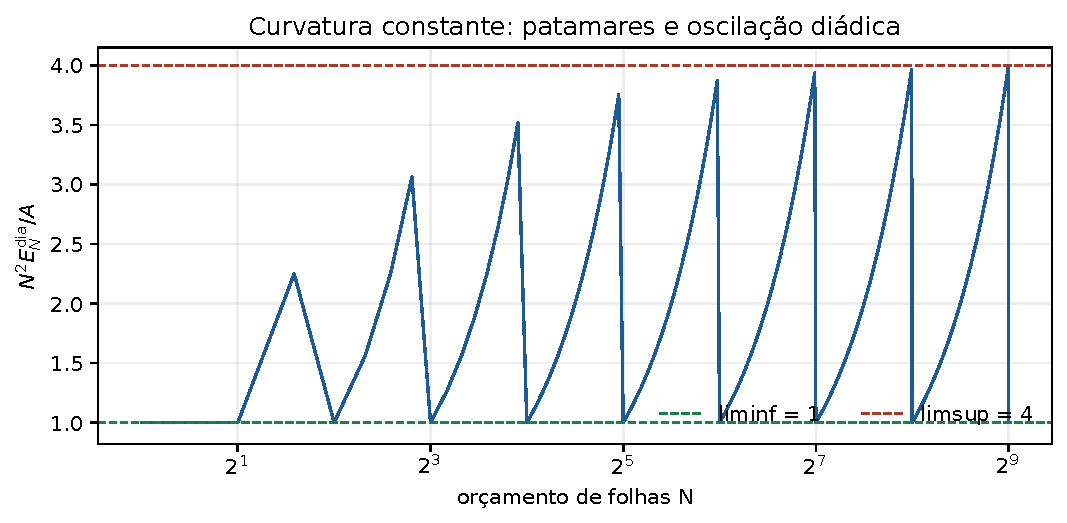
\includegraphics[width=.88\linewidth]{figuras/artigo_2/fig03_constante_quadratica.pdf}
 \caption{A normalização $N^2E_N^{\rm dia}/A$ reinicia em $1$ nas potências
 de dois e se aproxima de $4$ antes da potência seguinte.}
 \label{artigo_2:fig:quadratic-sawtooth}
\end{figure}

A \cref{artigo_2:tab:quadratic-exact} lista os valores racionais da lei, e a
\cref{artigo_2:fig:quadratic-sawtooth} exibe a oscilação normalizada entre as fases
diádicas consecutivas.

\subsection{Quadráticas por partes e lei de fase}

O caso seguinte separa a oscilação causada por uma única escala daquela
produzida por regiões com curvaturas diferentes.

% MAPA artigo_2:12.2
\begin{theorem}[contagem exata em uma malha diádica base]\label{map:artigo_2:12.2}
\label{artigo_2:thm:piecewise-quadratic-count}
Seja $\mathcal Q_{q_0}$ a partição uniforme de $K=[0,1]$ em células
$Q_i$ de comprimento $2^{-q_0}$. Suponha que $f\in C^1(K)$ seja quadrática
em cada $Q_i$ e
\[
 f''|_{\mathring Q_i}=\kappa_i\ne0,
 \qquad
 A_i=\frac{|\kappa_i||Q_i|^2}{8}.
\]
Existe $\varepsilon_0>0$ tal que, para
$0<\varepsilon<\varepsilon_0$,
\begin{equation}
 n_f(\varepsilon)
 =\sum_i2^{\lceil\log_4(A_i/\varepsilon)\rceil}.
 \label{artigo_2:eq:piecewise-count-law}
\end{equation}
Se $s=-\log_4\varepsilon$ e $a_i=\log_4A_i$, então
\begin{equation}
 \sqrt\varepsilon\,n_f(\varepsilon)
 =\Phi(s),
 \qquad
 \Phi(s)=\sum_i\sqrt{A_i}\,
 2^{\lceil s+a_i\rceil-(s+a_i)}.
 \label{artigo_2:eq:piecewise-phase-law}
\end{equation}
A função $\Phi$ é $1$-periódica e não constante. Portanto nem mesmo a
normalização em tolerância possui, em geral, um limite simples.
\end{theorem}

\begin{proof}
Todo ancestral da malha base que contém algum $Q_i$ é não afim, logo possui
erro local positivo. Como há apenas um número finito desses ancestrais,
escolha $\varepsilon_0$ menor que todos os seus erros e que todos os $A_i$.
O \cref{artigo_2:thm:threshold-optimality} obriga então a árvore de limiar a alcançar
cada $Q_i$. Dentro de $Q_i$, a identidade
\eqref{artigo_2:eq:quadratic-local-exact} mostra que são necessárias e suficientes
$2^{\lceil\log_4(A_i/\varepsilon)\rceil}$ folhas. Somar prova
\eqref{artigo_2:eq:piecewise-count-law}; a reescrita algébrica dá
\eqref{artigo_2:eq:piecewise-phase-law}. A periodicidade segue de
$\lceil s+1+a_i\rceil-(s+1+a_i)=\lceil s+a_i\rceil-(s+a_i)$.
Em qualquer intervalo aberto sem uma das finitíssimas fases de salto, todos
os tetos permanecem fixos e $\Phi$ é um múltiplo positivo de $2^{-s}$;
portanto é estritamente decrescente ali e não pode ser constante.
\end{proof}

% MAPA artigo_2:12.3
\begin{corollary}[fases sincronizadas]\label{map:artigo_2:12.3}
\label{artigo_2:cor:synchronized-phases}
Nas hipóteses do \cref{artigo_2:thm:piecewise-quadratic-count}, suponha ainda que
$A_i/A_j\in4^{\mathbb Z}$ para todos $i,j$. Então
\begin{equation}
 \liminf_{N\to\infty}N^2E_N^{\rm dia}(f)_\infty=\frac{I(f)^2}{8},
 \qquad
 \limsup_{N\to\infty}N^2E_N^{\rm dia}(f)_\infty=\frac{I(f)^2}{2}.
 \label{artigo_2:eq:synchronized-extremes}
\end{equation}
\end{corollary}

\begin{proof}
Seja $A_\ast=\min_iA_i>0$. Pela hipótese de sincronia, $A_i=A_\ast4^{\rho_i}$ com
$\rho_i\in\mathbb Z$, e a minimalidade de $A_\ast$ dá $\rho_i\ge0$. Ponha
$M=\sum_i2^{\rho_i}\ge1$.

Pelo \cref{artigo_2:thm:piecewise-quadratic-count}, existe $\varepsilon_0>0$ tal que,
para $0<\varepsilon<\varepsilon_1:=\min\{\varepsilon_0,A_\ast\}$,
$n_f(\varepsilon)=\sum_i2^{\lceil\log_4(A_i/\varepsilon)\rceil}$. Com
$D(\varepsilon)=\lceil\log_4(A_\ast/\varepsilon)\rceil$ e $\varepsilon<A_\ast$, vale
$\lceil\log_4(A_\ast4^{\rho_i}/\varepsilon)\rceil=\rho_i+D(\varepsilon)$, logo
\[
 n_f(\varepsilon)=M\,2^{D(\varepsilon)},
 \qquad
 D(\varepsilon)\le j\iff A_\ast4^{-j}\le\varepsilon .
\]

Fixe $R_0$ com $A_\ast4^{-R_0}<\varepsilon_1$ e, para $N\ge M2^{R_0}$, ponha
$j(N)=\lfloor\log_2(N/M)\rfloor\ge R_0$. Para $0<\varepsilon<\varepsilon_1$, o
\cref{artigo_2:thm:threshold-optimality} dá
$E_N^{\rm dia}(f)_\infty\le\varepsilon\iff n_f(\varepsilon)\le N\iff
M2^{D(\varepsilon)}\le N\iff D(\varepsilon)\le j(N)\iff A_\ast4^{-j(N)}\le\varepsilon$.
Como $A_\ast4^{-j(N)}<\varepsilon_1$, as duas quantidades têm os mesmos majorantes
em $(0,\varepsilon_1)$, e portanto
\[
 E_N^{\rm dia}(f)_\infty=A_\ast4^{-\lfloor\log_2(N/M)\rfloor}
 \qquad(N\ge M2^{R_0}).
\]
É a lei exata do \cref{artigo_2:thm:quadratic-dyadic-constant}, com $A$ substituído
por $A_\ast$ e o orçamento medido em unidades de $M$. Se
$M2^j\le N<M2^{j+1}$, então $M^2A_\ast\le N^2E_N^{\rm dia}(f)_\infty<4M^2A_\ast$;
o valor $M^2A_\ast$ é atingido em $N=M2^j$ e
$(M2^{j+1}-1)^2A_\ast4^{-j}\to4M^2A_\ast$. Logo
\[
 \liminf_{N\to\infty}N^2E_N^{\rm dia}(f)_\infty=M^2A_\ast,
 \qquad
 \limsup_{N\to\infty}N^2E_N^{\rm dia}(f)_\infty=4M^2A_\ast .
\]
Finalmente, no interior de cada $Q_i$ tem-se $|f''|=|\kappa_i|$, de modo que
\[
 I(f)=\sum_i\sqrt{|\kappa_i|}\,|Q_i|=\sum_i\sqrt{8A_i}
 =\sqrt{8A_\ast}\sum_i2^{\rho_i}=\sqrt{8A_\ast}\,M,
\]
isto é, $M^2A_\ast=I(f)^2/8$ e $4M^2A_\ast=I(f)^2/2$, o que prova
\eqref{artigo_2:eq:synchronized-extremes}. A demonstração usa apenas a contagem
exata do \cref{artigo_2:thm:piecewise-quadratic-count} e a periodicidade em
$4^{\mathbb Z}$; não recorre ao envelope do
\cref{artigo_2:thm:general-dyadic-envelope}, cuja hipótese $C^2$ uma quadrática por
partes pode não satisfazer.
\end{proof}

A presença de sinais diferentes entre os $\kappa_i$ não altera essas
fórmulas: os erros locais dependem de $|\kappa_i|$. Para uma função global
$C^2$, uma mudança de sinal passa por zeros e a lei finita por fases deixa de
ser literalmente aplicável, mas o \cref{artigo_2:thm:general-dyadic-envelope} continua
válido sem alteração.

\begin{figure}[t]
 \centering
 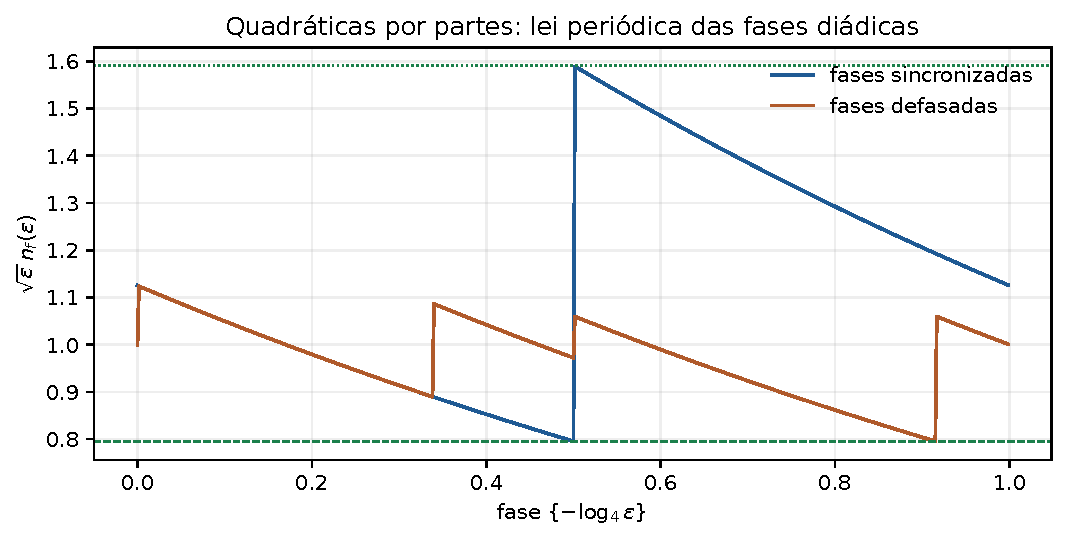
\includegraphics[width=.88\linewidth]{figuras/artigo_2/fig04_fases_piecewise.pdf}
 \caption{A lei \eqref{artigo_2:eq:piecewise-phase-law} em uma família sincronizada e
 outra defasada. Deslocar $-\log_4\varepsilon$ por uma unidade repete
 exatamente o perfil.}
 \label{artigo_2:fig:piecewise-phases}
\end{figure}

A sincronização e a defasagem previstas por
\eqref{artigo_2:eq:piecewise-phase-law} são comparadas na
\cref{artigo_2:fig:piecewise-phases}.

\subsection{Implementação e auditorias independentes}

O programa \path{verificacao/constante_diadica.py} implementa duas rotas que não
reutilizam a mesma recorrência: a árvore menos refinada do
\cref{artigo_2:thm:threshold-optimality} e uma programação dinâmica por número exato
de folhas,
\begin{equation}
 D(J,1)=e_f(J),\qquad
 D(J,n)=\min_{n_L+n_R=n}\max\{D(J_L,n_L),D(J_R,n_R)\}.
 \label{artigo_2:eq:independent-tree-dp}
\end{equation}
Para funções quadráticas por partes, $f$, $f'$, todos os pontos críticos e
todos os erros locais são calculados com \texttt{Fraction}. A fórmula
quadrática foi comparada com \eqref{artigo_2:eq:independent-tree-dp} para
$1\le N\le14$; a lei por partes foi confrontada com a construção explícita
do limiar em 14 escalas e a inversão do limiar foi comparada com a DP para
$1\le N\le12$.

Os dois diagnósticos $C^2$ usam apenas ponto flutuante determinístico para
avaliar extremos analíticos: $e^x$, cuja curvatura é estritamente positiva,
e $(x-1/2)^3$, cuja segunda derivada muda de sinal. Eles não participam de
nenhuma prova de igualdade; verificam apenas que os valores finitos
$\varepsilon n_f(\varepsilon)^2$ permanecem dentro do envelope teórico nas
$400$ tolerâncias examinadas.

% MAPA artigo_2:12.4
\begin{remark}[agudeza uniforme e comportamento pontual]\label{map:artigo_2:12.4}
\label{artigo_2:rem:envelope-not-pointwise}
O \cref{artigo_2:thm:general-dyadic-envelope} é agudo \emph{uniformemente sobre a
classe} $C^2$: a mesma função quadrática do
\cref{artigo_2:thm:quadratic-dyadic-constant} realiza $I(f)^2/8$ e $I(f)^2/2$ ao longo
de subsequências. Logo as duas constantes são ótimas em teoremas uniformes
sobre $C^2$. Para uma função fixa, o conjunto de acumulação pode ser um
subconjunto próprio do envelope.

No modelo finito do \cref{artigo_2:thm:piecewise-quadratic-count}, essa distinção pode
ser tornada exata. Ponha $w_i=\sqrt{A_i}$ e considere os resíduos de
$a_i=\log_4A_i$ módulo $1$. Cada fator
\[
 g(s+a_i)=2^{\lceil s+a_i\rceil-(s+a_i)}
\]
pertence a $[1,2)$ e vale $1$ precisamente quando $s+a_i\in\mathbb Z$. Se os
resíduos não são todos iguais, não existe fase que torne simultaneamente
todos os fatores iguais a $1$, nem uma sequência de fases que os faça tender
simultaneamente a $2$. Como há apenas um número finito de fases de salto no
círculo, existem $\delta_-,\delta_+>0$ tais que
\[
 \frac{I(f)}{\sqrt8}+\delta_-
 \le \Phi(s)
 \le \frac{I(f)}{\sqrt2}-\delta_+
 \qquad(s\in\mathbb R).
\]
Assim, a normalização dual $\varepsilon n_f(\varepsilon)^2$ permanece
estritamente dentro do envelope para todas as tolerâncias suficientemente
pequenas nessa família defasada. No caso sincronizado, a condição
$A_i/A_j\in4^{\mathbb Z}$ do \cref{artigo_2:cor:synchronized-phases} alinha os
resíduos e permite recuperar os extremos.

A prova finita usa o número discreto de fases de salto e, portanto, é
específica da curvatura quadrática por partes. A
\cref{artigo_2:tab:smooth-diagnostics} registra que, em $400$ tolerâncias entre
$10^{-3}$ e $10^{-10}$, os dois exemplos suaves permanecem estritamente no
interior. A caracterização, para $f$ dada, do conjunto exato de acumulação de
$N^2E_N^{\rm dia}(f)_\infty$ dentro de
$[I(f)^2/8,\allowbreak I(f)^2/2]$ constitui o problema de fases para curvatura variável.
\end{remark}

\begin{table}[t]
 \centering
 \caption{Diagnósticos determinísticos em 400 tolerâncias entre
 $10^{-3}$ e $10^{-10}$. As colunas externas são teóricas.}
 \label{artigo_2:tab:smooth-diagnostics}
 \small
 \begin{tabular}{lrrr}
\toprule
função & $I(f)^2/8$ & faixa observada de $\varepsilon n_f(\varepsilon)^2$ & $I(f)^2/2$ \\
\midrule
$e^x$ & 0{,}210420 & [0{,}339008; 0{,}515293] & 0{,}841679 \\
$(x-\frac{1}{2})^3$ & 0{,}166667 & [0{,}275877; 0{,}417099] & 0{,}666667 \\
\bottomrule
\end{tabular}

\end{table}

\begin{figure}[t]
 \centering
 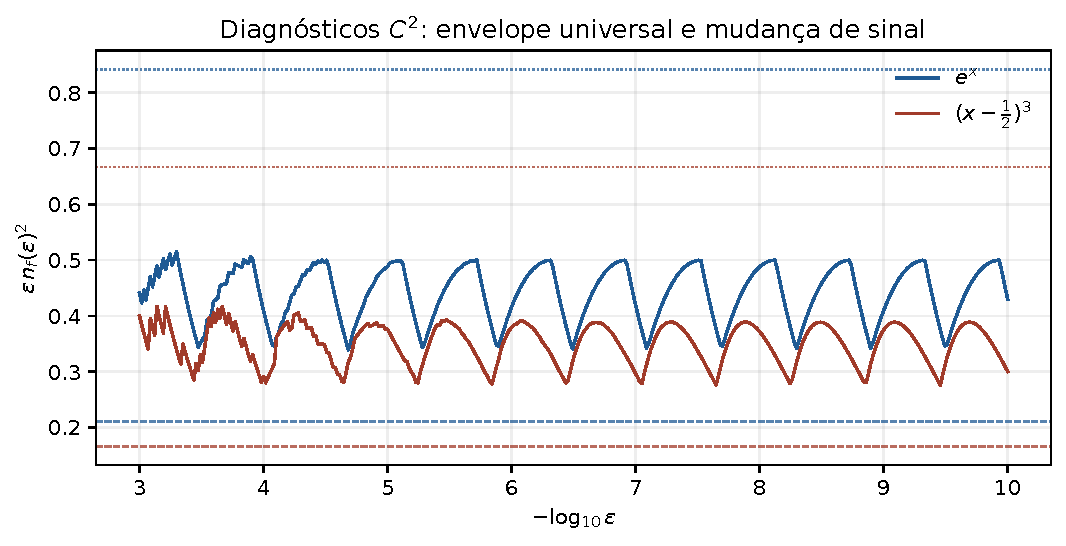
\includegraphics[width=.88\linewidth]{figuras/artigo_2/fig05_envelope_c2.pdf}
 \caption{Diagnósticos para curvatura positiva e para mudança de sinal. As
 linhas tracejadas e pontilhadas são, respectivamente, $I(f)^2/8$ e
 $I(f)^2/2$.}
 \label{artigo_2:fig:c2-envelope}
\end{figure}

Os dois exemplos suaves da \cref{artigo_2:fig:c2-envelope} permanecem dentro do
envelope teórico em todas as tolerâncias auditadas.

\begin{table}[t]
 \centering
 \caption{Auditoria executável das constantes diádicas.}
 \label{artigo_2:tab:dyadic-constants-audit}
 \small
 \begin{tabularx}{\linewidth}{@{}Xr@{}}
\toprule
Verificação & resultado \\
\midrule
Fórmula quadrática $=$ DP independente & true \\
Limiar quadrático $=$ contagem fechada & true \\
Contagem por partes $=$ árvore de limiar & true \\
DP por partes $=$ inversão do limiar & true \\
Fases sincronizadas atingem os dois extremos & true \\
Diagnóstico $C^2$ positivo dentro do envelope & true \\
Mudança de sinal dentro do envelope & true \\
Varreduras suaves estritamente interiores (400 pontos) & true \\
Execução sem números pseudoaleatórios & true \\
\bottomrule
\end{tabularx}

\end{table}

A \cref{artigo_2:tab:dyadic-constants-audit} reúne, em uma única trilha, as
identidades exatas e os testes independentes desta seção.

\subsection{Compatibilidade com a altura aritmética}

Os teoremas desta seção permitem todos os descendentes da raiz. Na biblioteca
$\Library$, uma malha uniforme de profundidade relativa $r$ em
$K=J_{k_0,m_0}$, $m_0\ge0$, só está espacialmente disponível quando
\[
 H\ge k_0+r+1,
 \qquad H\ge2^r(m_0+1)
\]
pela \cref{artigo_2:prop:translation-obstruction}. Como as escalas relevantes têm
$2^r\asymp N$, a segunda condição já força $H=\Omega(N(m_0+1))$, antes de
se contabilizar a altura necessária para racionalizar os valores nodais.
Assim, a passagem de \eqref{artigo_2:eq:budget-envelope} para uma agenda $H(N)$ inclui
esse acoplamento geométrico.

Para cada árvore fixa, o teorema de racionalização da \cref{artigo_2:sec:assemblies}
aproxima os valores nodais reais por racionais compartilhados e aproxima
$P_\Lambda f$ arbitrariamente bem por uma montagem da biblioteca. Os
interpolantes pertencem, portanto, à aderência quando a altura cresce. O
problema interpolatório \eqref{artigo_2:eq:optimal-dyadic-interpolation} e o melhor
erro racional com deslocamentos nodais são objetos distintos; a constante
assintótica do segundo sob uma agenda fixa de altura permanece em aberto.
\section{Verificações de codificação e entropia}
\label{artigo_2:sec:coding-validation}
Os registros desta seção acompanham o programa \path{verificacao/reproduzir_curvas.py}. As verificações usam aritmética racional para os formatos e parâmetros; as curvas e as sondas de distorção são diagnósticos numéricos.

\subsection{Roundtrip dos formatos de codificação}

Os codificadores de \cref{artigo_2:subsec:coding-formats} e seus decodificadores foram
executados em $4096$ montagens racionais de teste. Em
todos os casos, o fluxo atômico recuperou a assinatura linear por partes e os
dois fluxos ReLU recuperaram exatamente cada \texttt{Fraction} da rede. Foram
também verificadas, parâmetro a parâmetro, as cotas
\eqref{artigo_2:eq:slope-jump-height}--\eqref{artigo_2:eq:intercept-height}.

A fatia $N=2$ da família de \eqref{artigo_2:eq:coding-gap-family} permite comparar os
comprimentos sem regressão nem ajuste assintótico. A
\cref{artigo_2:tab:codificacoes-pt} dá os valores exatos e a
\cref{artigo_2:fig:codificacoes-pt} mostra as ordens de crescimento:
\begin{table}[t]
\centering
\caption{Comprimentos exatos dos três fluxos prefix-free na família crítica.}
\label{artigo_2:tab:codificacoes-pt}
\small
\begin{tabular}{rrrrr}
\toprule
$H$ & $L_{\rm atom}$ & $L_{\rm ReLU,str}$ & $L_{\rm ReLU,rat}$ & razão rat./str.\\
\midrule
4 & 29 & 31 & 35 & 1{,}129\\
8 & 33 & 35 & 51 & 1{,}457\\
16 & 37 & 39 & 83 & 2{,}128\\
32 & 41 & 43 & 147 & 3{,}419\\
64 & 45 & 47 & 275 & 5{,}851\\
128 & 49 & 51 & 531 & 10{,}412\\
\bottomrule
\end{tabular}

\end{table}

\begin{figure}[t]
 \centering
 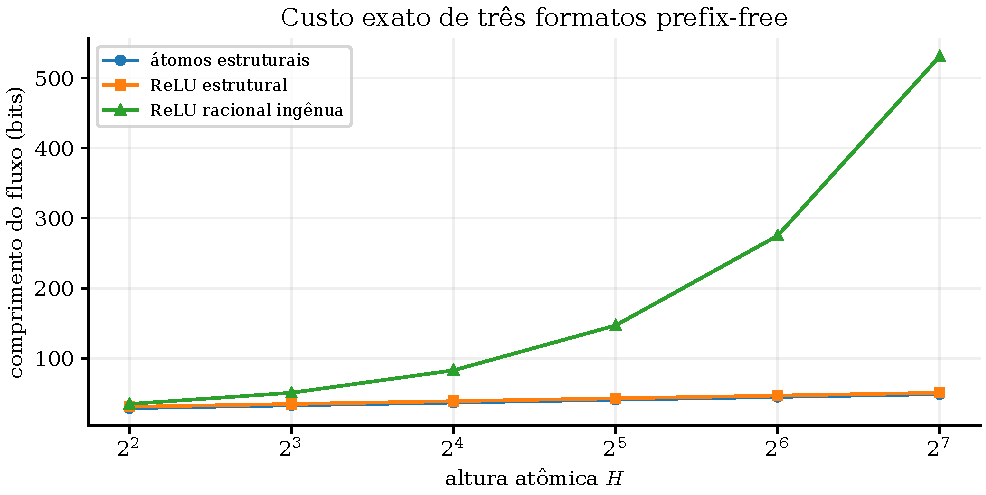
\includegraphics[width=.82\linewidth]{figuras/artigo_2/fig08_codificacoes.pdf}
 \caption{O par diádico estrutural mantém o custo logarítmico; expandir o
 denominador $2^k$ como parte de uma fração racional produz a sobrecarga
 linear prevista pelo \cref{artigo_2:thm:coding-formats}.}
 \label{artigo_2:fig:codificacoes-pt}
\end{figure}


\subsection{Restrição de curvatura e codebook sem fator logarítmico}

A contagem de \eqref{artigo_2:eq:code-length} restringe os vetores admissíveis pelas diferenças segundas, mantendo os mesmos átomos e grades.

O script avalia quatro sondas determinísticas. Cada uma é reescalada pelo fator
\[\min\{R/\|f\|_\infty,\,M/\|f''\|_\infty\}\]
para que pertença a
$\mathcal F_{R,M}$ com $R=1$ e $M=8$: a quadrática que satura as duas
restrições simultaneamente, dois harmônicos e a função de Runge reescalada.
Antes do reescalamento, a sonda de Runge tem $\|f''\|_\infty=200$. Para cada tolerância, verifica-se que
$\varepsilon/2<\delta\le\varepsilon$, que $Mh^2\le4\varepsilon$, que o erro
nodal não excede $\delta/2$, que valores adjacentes são distintos, que cada
peça é um átomo de inclinação racional não nula e que a distorção fica dentro
de $\varepsilon$.

\begin{table}[t]
\centering
\caption{Sucessores admissíveis por nó e comprimento do índice global reescalado.}
\label{artigo_2:tab:codebook-pt}
\small
\begin{tabular}{rrrrrr}
\toprule
$\varepsilon$ & $N$ & sucessores & distorção & $L_\varepsilon^{\mathrm{global}}\sqrt{\varepsilon}$ & antigo $\cdot\sqrt{\varepsilon}$\\
\midrule
$6{,}250\,10^{-2}$ & 8   & 9 & $3{,}90\,10^{-2}$ & $10{,}68$ & $13{,}50$\\
$1{,}562\,10^{-2}$ & 16  & 9 & $9{,}68\,10^{-3}$ & $10{,}34$ & $17{,}00$\\
$3{,}906\,10^{-3}$ & 32  & 9 & $2{,}26\,10^{-3}$ & $10{,}00$ & $20{,}62$\\
$9{,}766\,10^{-4}$ & 64  & 9 & $6{,}98\,10^{-4}$ & $9{,}74$  & $24{,}38$\\
$2{,}441\,10^{-4}$ & 128 & 9 & $1{,}62\,10^{-4}$ & $9{,}56$  & $28{,}22$\\
\bottomrule
\end{tabular}
\end{table}

Na \cref{artigo_2:tab:codebook-pt}, O número de sucessores
admissíveis por nó, dados os dois valores anteriores, é $9$ em todas as
tolerâncias --- abaixo da constante $K=25$ usada na demonstração, que é
portanto conservadora e não ajustada aos dados. As duas últimas colunas são o
diagnóstico do fator logarítmico: o comprimento do índice global da cota por diferenças segundas,
multiplicado por $\sqrt{\varepsilon}$, permanece limitado e até decresce
levemente, enquanto a contagem termo a termo de cada nó cresce
como $\log(1/\varepsilon)$ na mesma normalização. É exatamente a diferença
entre $O(\varepsilon^{-1/2})$ e $O(\varepsilon^{-1/2}\log(1/\varepsilon))$.


\subsection{Contagem de átomos e otimalidade minimax do endereço}

A \cref{artigo_2:tab:enderecos-pt} confronta a contagem exata $|\Library_H|$ com as cotas do
\cref{artigo_2:lem:atom-count} e compara, no pior caso sobre $\Library_H$, o endereço
aritmético $n$ do gerador $\Gamma$ com o endereço $n^\sharp$ da enumeração por
altura da \cref{artigo_2:def:sharp}. A coluna final registra a cota inferior universal,
quanto ao endereçamento sob o calibre fixado, do
\cref{artigo_2:thm:address-lower}. Os expoentes empíricos, obtidos por regressão de
$\log_2(\cdot)$ contra $\log_2H$ nas últimas linhas, aproximam $6$ para
$|\Library_H|$ e $n^\sharp$ e $8$ para $n$, como previsto.

\begin{table}[t]
\centering
\caption{Contagem de átomos por altura e comprimento de endereço no pior caso.}
\label{artigo_2:tab:enderecos-pt}
\small
\begin{tabular}{rrrrr}
\toprule
$H$ & $|\Library_H|$ & $|\Library_H|/(18H^6)$ & $\max n$ ($\Gamma$) & $\max n^\sharp=$ cota inf.\\
\midrule
2 & 252 & 0{,}2188 & 3231 & 251\\
3 & 3150 & 0{,}2401 & 87\,127 & 3149\\
4 & 14\,168 & 0{,}1922 & 519\,638 & 14\,167\\
6 & 142\,692 & 0{,}1699 & 9\,515\,572 & 142\,691\\
8 & 897\,840 & 0{,}1903 & 113\,062\,957 & 897\,839\\
12 & 9\,192\,456 & 0{,}1710 & 2\,233\,224\,112 & 9\,192\,455\\
16 & 50\,315\,232 & 0{,}1666 & 20\,668\,188\,575 & 50\,315\,231\\
24 & 582\,320\,976 & 0{,}1693 & 534\,070\,940\,833 & 582\,320\,975\\
32 & 3\,378\,271\,680 & 0{,}1748 & 5\,622\,328\,883\,731 & 3\,378\,271\,679\\
48 & 36\,947\,682\,720 & 0{,}1678 & 131\,374\,552\,971\,847 & 36\,947\,682\,719\\
64 & 206\,341\,325\,696 & 0{,}1668 & 1\,289\,353\,431\,661\,883 & 206\,341\,325\,695\\
\bottomrule
\end{tabular}

\end{table}

A \cref{artigo_2:fig:enderecos-pt} torna visível a diferença entre os expoentes do
gerador aritmético e da enumeração por cascas, sempre para o calibre
\eqref{artigo_2:eq:atom-height}.

\begin{figure}[t]
 \centering
 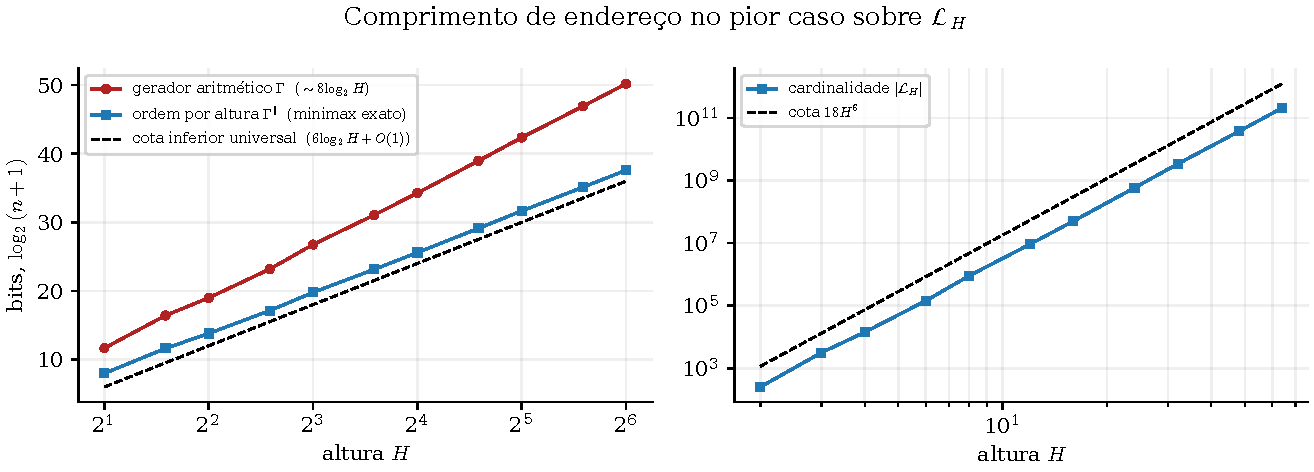
\includegraphics[width=.92\linewidth]{figuras/artigo_2/fig06_enderecos.pdf}
 \caption{Comprimento de endereço no pior caso sobre $\Library_H$. A enumeração
 por altura $\Gamma^\sharp$ acompanha a cota inferior relativa a $\Library_H$ com uma folga
 limitada; o gerador aritmético $\Gamma$ paga um fator constante $4/3$ no
 expoente em troca de inversa em forma fechada.}
 \label{artigo_2:fig:enderecos-pt}
\end{figure}

Foi ainda verificada, para $0\le n^\sharp<20\,000$, a bijetividade de
$\Gamma^\sharp$ nos dois sentidos e a coincidência dos conjuntos
$\Gamma(\{0,\ldots,N\})$ e $\Gamma^\sharp(\{0,\ldots,N'\})$ quando restritos a
uma mesma casca de altura.

\FloatBarrier
\clearpage
\section{Conclusão}
O calibre adotado produz $\Theta(H^6)$ átomos e uma enumeração por altura que minimiza exatamente o pior índice. Os três formatos de codificação explicitam como a representação dos diádicos altera o comprimento da palavra. A restrição de curvatura reduz a cardinalidade do codebook e realiza a ordem entrópica $\varepsilon^{-1/2}$.

Na seleção, os valores racionais de fronteira fornecem estados suficientes para preservar continuidade e admissibilidade. As recorrências calculam o mínimo do catálogo, com desempate canônico e custos separados em operações e bits. A estabilização sob truncagem exige que o mínimo global seja atingido; a seleção exata pode ser descontínua em empates.

Para a interpolação estritamente diádica, o erro normalizado admite o envelope $[I(f)^2/8,\allowbreak I(f)^2/2]$. Curvatura constante e quadráticas por partes explicitam as fases responsáveis pela oscilação. A caracterização das fases para curvatura variável e o efeito de uma agenda fixa sobre o melhor erro racional permanecem questões distintas dos resultados interpolatórios demonstrados.




% IV | fonte original: artigos/artigo_3/Artigo_3.tex
\volumeparte{Agendas de altura e teoria direta--inversa}
% Reconstruído de artigos/artigo_3/Artigo_3.tex


\renewcommand{\abstractname}{Resumo}
\begin{abstract}Estudamos taxas de aproximação por montagens racionais sob agendas de altura aritmética. O funcional de melhor erro define estratos, mas falha em ser homogêneo por escalares reais. Construímos aproximantes em malhas diádicas com altura suficiente de ordem $N^{\max\{1,s\}}$, com fator logarítmico para a somabilidade crítica quando $q<\infty$, e cotas uniformes sobre bolas de Besov. Para erro bruto de ordem $N^{-\alpha}$ e crescimento de Lipschitz $N^\gamma$, obtemos regularidade inversa de ordem $\alpha/(\alpha+\gamma)$; um pente de tendas demonstra agudeza na biblioteca original quando $0<\alpha\le\gamma$. A extensão marcada caracteriza a reversibilidade exata com redes ReLU rasas racionais, e uma construção quantizada trata parâmetros reais. Ao somar ao erro a segunda diferença do aproximante na escala correspondente, obtemos uma caracterização direta e inversa das classes de Besov. A cota inversa desse funcional é universal; a direção direta fornece o controle aritmético específico da biblioteca.\end{abstract}
\renewcommand{\abstractname}{Abstract}
\begin{abstract}We study approximation rates of rational assemblies under arithmetic height schedules. The best-error functional defines approximation strata but fails real homogeneity. We construct dyadic approximants with sufficient height of order $N^{\max\{1,s\}}$, with a logarithmic factor for critical summability when $q<\infty$, and uniform bounds on Besov balls. A raw rate $N^{-\alpha}$ under Lipschitz growth $N^\gamma$ implies inverse regularity of order $\alpha/(\alpha+\gamma)$; a tent comb proves sharpness in the original library for $0<\alpha\le\gamma$. A marked completion characterizes exact reversal of rational shallow ReLU networks, while quantization handles real parameters. Adding the approximant's second-order modulus at the matching scale yields a direct and inverse characterization of Besov classes. The inverse bound is universal; the direct construction supplies the arithmetic control specific to the library.\end{abstract}
\renewcommand{\abstractname}{Resumo}
\section{Introdução}
Uma função linear por partes pode ter erro de aproximação nulo em todas as escalas posteriores e conservar quinas. Por isso, uma taxa rápida do melhor erro, tomada isoladamente, não caracteriza suavidade de ordem superior a um. Sob restrições aritméticas, soma-se outra questão: o catálogo de altura fixa não é invariante por multiplicação por escalares reais.

Este artigo formula as classes de aproximação compatíveis com essa estrutura e estabelece suas relações com espaços de Besov. A biblioteca e os resultados de custo e seleção foram desenvolvidos nos dois primeiros artigos \citep{artigo_2-oliveiraI,artigo_2-oliveiraII}. A teoria de aproximação não linear e os teoremas diretos e inversos fornecem o contexto funcional \citep{artigo_1-devore1998,artigo_2-devorepopov1988,artigo_2-petrushev1988,artigo_2-devorelorentz1993}. Funcionais de realização relacionam aproximação restrita e módulos de suavidade \citep{artigo_2-hristovivanov1990}. As relações com redes ReLU e restrições de pesos são tratadas em \citet{artigo_2-devorehaninpetrova2021,artigo_1-daubechies2022,artigo_2-gribonval2022,artigo_2-grohs2023,artigo_1-guhring2021}.

O primeiro resultado acompanha o denominador racional comum e fornece agendas suficientes de altura. O segundo relaciona erro bruto e crescimento das inclinações a uma regularidade inversa com perda. A agudeza na biblioteca original é demonstrada na faixa $0<\alpha\le\gamma$. A reversibilidade exata com redes rasas exige parâmetros racionais e quebras diádicas; a extensão marcada conserva explicitamente o suporte de peças constantes.

Para recuperar uma caracterização de Besov, somamos ao erro o módulo de segunda ordem do aproximante na escala pareada. A desigualdade inversa vale para qualquer família de funções. A racionalização estabelece a direção direta com altura controlada, inclusive uniformemente sobre bolas. As igualdades obtidas são igualdades de conjuntos sob as agendas declaradas.

\section{Biblioteca, altura e erro de aproximação}
\label{artigo_3:sec:baseIII}
Usamos a biblioteca racional do primeiro artigo \citep{artigo_2-oliveiraI} e o controle de recursos do segundo \citep{artigo_2-oliveiraII}. Para $r=p/q$ reduzido, $q>0$, ponha $\height(r)=\max\{|p|,q\}$. Um átomo em $J_{k,m}=[m2^{-k},(m+1)2^{-k}]$ tem a forma
\begin{equation}
 \ell(x)=y_0+s(x-x_{k,m}),\quad x_{k,m}=(m+1/2)2^{-k},\quad y_0\in\mathbb Q,\ s\in\Qstar,
 \label{artigo_3:eq:inherited-atom}
\end{equation}
e altura
\begin{equation}
 \height_{\rm at}=\max\{2,k+1,|m|+1,\height(y_0),\height(s)\}.
 \label{artigo_3:eq:inherited-height}
\end{equation}
Fixe uma raiz $K=J_{k_0,m_0}$. Uma montagem é uma função contínua que coincide com um átomo em cada folha de uma árvore diádica finita com raiz $K$. Escreva $\Aclass_{N,H}(K)$ para as funções que admitem uma mesma representação com até $N$ folhas e altura máxima $H$, e
\[
 E_{N,H}^{\Library}(f)_\infty=\inf_{g\in\Aclass_{N,H}(K)}\|f-g\|_{\infty,K}.
\]
Os catálogos são finitos, pois a altura limita todas as coordenadas atômicas. Ao longo de orçamentos cofinalmente crescentes, suas montagens são densas em $C(K)$.

Na malha uniforme de $n=2^r$ folhas, os índices são $(k_0+r,2^rm_0+j)$, $0\le j<n$. Se $m_0\ge0$, a admissibilidade geométrica de todas as folhas equivale a $k_0+r+1\le H$ e $n(m_0+1)\le H$. Em particular, em $[0,1]$ a malha uniforme exige $H\ge n$.

O segundo artigo demonstra que, para $\mathcal F_{R,M}=\{f\in C^2[0,1]:\|f\|_\infty\le R,\ \|f''\|_\infty\le M\}$ e $C_H=\max\{4(R+1),2(4R+M/2+1)\}$,
\[
 E_{N,\lceil C_HN^2\rceil}^{\Library}(f)_\infty<\frac{M+4}{2N^2},\qquad N\ge2.
\]
A construção usa valores nodais racionais em grades alternadas, preserva inclinações não nulas e admite $O_{R,M}(N\log(2N))$ bits nos formatos atômico, ReLU estrutural e ReLU racional. Esses resultados fornecem o endpoint $C^2$ usado adiante.

\section{Classes de aproximação sob uma agenda de altura}
\label{artigo_3:sec:approximation-classes}

O número de folhas e a altura aritmética desempenham papéis independentes. A
racionalização por denominador comum absorve o fator da malha e fornece
altura suficiente $N^2$ no caso $s=2$. Ao mesmo tempo, catálogos racionais de
altura fixa falham em ser invariantes por escalares reais. O funcional
associado será, por isso, formulado como funcional de taxa e sua obstrução de
homogeneidade será demonstrada explicitamente.

\subsection{Erro apontado e funcional de taxa}

Seja $H:\mathbb N\to\mathbb N$, $H(N)\ge2$, uma agenda não decrescente.
Estenda a notação $\Aclass_{N,H}(K)$ ao caso $N=1$ pela mesma
definição: no máximo uma folha e altura no máximo $H$. Essa classe pode não
conter a função nula, pois a
biblioteca exclui inclinações nulas. Para obter um erro com ponto-base sem
alterar nenhum aproximante não nulo, ponha
\begin{equation}
 \Sigma_N^{\Library,H}(K)
 :=\{0\}\cup\Aclass_{N,H(N)}(K),
 \qquad
 e_N^{\Library,H}(f)
 :=\inf_{g\in\Sigma_N^{\Library,H}(K)}\|f-g\|_{\infty,K}.
 \label{artigo_3:eq:pointed-error}
\end{equation}
Em termos do erro conjunto da seção de custos do segundo artigo \citep{artigo_2-oliveiraII}, estendido pela mesma fórmula
ao caso $N=1$,
\begin{equation}
 e_N^{\Library,H}(f)
 =\min\bigl\{\|f\|_{\infty,K},
 E_{N,H(N)}^{\Library}(f)_\infty\bigr\}.
 \label{artigo_3:eq:pointed-inherited}
\end{equation}
A origem completa o esquema apontado usado para medir taxas.

% MAPA artigo_3:3.1
\begin{proposition}[aninhamento da agenda]\label{map:artigo_3:3.1}
\label{artigo_3:prop:schedule-nesting}
Se $H$ é não decrescente, então
\begin{equation}
 \Sigma_N^{\Library,H}(K)
 \subseteq\Sigma_{N+1}^{\Library,H}(K)
 \quad\text{e}\quad
 e_{N+1}^{\Library,H}(f)\le e_N^{\Library,H}(f)\le\|f\|_\infty.
 \label{artigo_3:eq:schedule-nesting}
\end{equation}
Para cada $N$, o ínfimo em \eqref{artigo_3:eq:pointed-error} é atingido.
\end{proposition}

\begin{proof}
Uma representação com no máximo $N$ folhas e altura no máximo $H(N)$
continua admissível sob os limites $N+1$ e $H(N+1)$. A função nula pertence
a ambas as classes. Isso prova as inclusões e as desigualdades. O calibre de
altura limita escala, translação, valor central e inclinação; portanto há
somente um número finito de átomos e de árvores admissíveis. Assim
$\Sigma_N^{\Library,H}(K)$ é finito e a distância mínima é atingida.
\end{proof}

A definição de classes por sequências de melhores erros é padrão na teoria de
espaços de aproximação não linear \citep{artigo_1-devore1998}. O funcional seguinte
acrescenta a essa construção o catálogo apontado e a agenda aritmética de
altura.

Para $\alpha>0$ e $0<q\le\infty$, defina o \emph{funcional de taxa}
\begin{align}
 \mathfrak a_{\alpha,q}^{\Library,H}(f)
 &:=\left(\sum_{N=1}^{\infty}
       \bigl[N^\alpha e_N^{\Library,H}(f)\bigr]^q\frac1N
       \right)^{1/q}, &&0<q<\infty,
 \label{artigo_3:eq:rate-functional-finite}\\
 \mathfrak a_{\alpha,\infty}^{\Library,H}(f)
 &:=\sup_{N\ge1}N^\alpha e_N^{\Library,H}(f).
 \label{artigo_3:eq:rate-functional-infty}
\end{align}
Escreva
\begin{equation}
 \mathscr A_{q}^{\alpha}(\Library,H)
 :=\{f\in C(K):\mathfrak a_{\alpha,q}^{\Library,H}(f)<\infty\}.
 \label{artigo_3:eq:approximation-stratum}
\end{equation}
O termo \emph{classe} ou \emph{estrato} será usado para
\eqref{artigo_3:eq:approximation-stratum}; \emph{espaço quase-normado} será reservado
a situações em que homogeneidade e quase-triângulo tenham sido efetivamente
provados. Essa distinção é necessária no catálogo presente e não ocorre
automaticamente a partir da literatura de esquemas cônicos ou de redes
\citep{artigo_2-gribonval2022,artigo_2-grohs2023}.

% MAPA artigo_3:3.2
\begin{theorem}[redução exata às escalas diádicas]\label{map:artigo_3:3.2}
\label{artigo_3:thm:dyadic-rate-equivalence}
Para toda agenda não decrescente, $\alpha>0$ e $0<q\le\infty$,
\begin{equation}
 \mathfrak a_{\alpha,q}^{\Library,H}(f)
 \asymp_{\alpha,q}
 \left\|\bigl(2^{r\alpha}
 e_{2^r}^{\Library,H}(f)\bigr)_{r\ge0}\right\|_{\ell^q},
 \label{artigo_3:eq:dyadic-rate-equivalence}
\end{equation}
com a interpretação usual por supremo quando $q=\infty$. As constantes não
dependem de $f$ nem de $H$.
\end{theorem}

\begin{proof}
No bloco $2^r\le N<2^{r+1}$, a monotonicidade fornece
\[
 e_{2^{r+1}}^{\Library,H}(f)
 \le e_N^{\Library,H}(f)
 \le e_{2^r}^{\Library,H}(f),
\]
enquanto $2^{r\alpha}\le N^\alpha<2^{(r+1)\alpha}$ e
\[
 \sum_{N=2^r}^{2^{r+1}-1}\frac1N\asymp1.
\]
Somar as duas estimativas de bloco e deslocar o índice inferior por uma
unidade prova \eqref{artigo_3:eq:dyadic-rate-equivalence}. Para $q=\infty$, basta
tomar o supremo nos mesmos blocos.
\end{proof}

\subsection{Obstrução de homogeneidade}

% MAPA artigo_3:3.3
\begin{proposition}[falha exata de homogeneidade]\label{map:artigo_3:3.3}
\label{artigo_3:prop:nonhomogeneous-functional}
Suponha $K=[0,1]$ e $H(1)\ge2$. O funcional
$\|f\|_\infty+\mathfrak a_{\alpha,q}^{\Library,H}(f)$ não é homogêneo sobre
$C(K)$ e, portanto, não é uma quase-norma. Mais precisamente, para
$f(x)=x$ e $c=\sqrt2$,
\begin{equation}
 \mathfrak a_{\alpha,q}^{\Library,H}(f)=0,
 \qquad
 \mathfrak a_{\alpha,q}^{\Library,H}(cf)>0.
 \label{artigo_3:eq:nonhomogeneous-certificate}
\end{equation}
\end{proposition}

\begin{proof}
A função $f(x)=x$ é o átomo $(k,m,y_0,s)=(0,0,1/2,1)$, de altura $2$.
Logo $f\in\Sigma_N^{\Library,H}(K)$ para todo $N$ e todos os erros de
$f$ são nulos. Por outro lado, toda função não nula em
$\Sigma_1^{\Library,H}(K)$ possui inclinação racional em $[0,1]$, enquanto
$cf$ possui inclinação irracional $\sqrt2$. Como o primeiro catálogo é
finito, $cf$ tem distância estritamente positiva a ele. Assim o termo
$N=1$ de \eqref{artigo_3:eq:rate-functional-finite}, ou o mesmo termo no supremo,
é positivo. Consequentemente,
\[
 \|cf\|_\infty+\mathfrak a_{\alpha,q}^{\Library,H}(cf)
 >|c|\bigl(\|f\|_\infty+
 \mathfrak a_{\alpha,q}^{\Library,H}(f)\bigr).
\]
\end{proof}

% MAPA artigo_3:3.4
\begin{remark}[estrutura aritmética do funcional]\label{map:artigo_3:3.4}
\label{artigo_3:rem:quasinorm-scope}
Adicionar $0$ fornece o ponto-base, enquanto a obstrução de homogeneidade real
permanece. O fecho cônico ou o envoltório linear admite escalares reais
externos e elimina o custo aritmético medido por $H$. Assim, os objetos
naturais são os estratos \eqref{artigo_3:eq:approximation-stratum} e seus funcionais de
taxa.
\end{remark}

\section{Teoremas diretos e agendas de altura}
\label{artigo_3:sec:direct-height}

O paradigma de teoremas diretos e inversos tem antecedentes tanto na
aproximação por splines e em espaços de Besov quanto na aproximação por funções
racionais \citep{artigo_2-petrushev1988,artigo_2-petrushevpopov1987}. Nesta última expressão,
``racional'' significa quociente de polinômios, e não a aritmética dos
coeficientes da biblioteca; o elemento novo desta seção é acompanhar
explicitamente a altura desses coeficientes.

Fixe a raiz diádica $K=J_{k_0,m_0}$ e escreva $L=|K|=2^{-k_0}$. Para
$f\in C(K)$, defina
\begin{align}
 \omega_1(f,t)_{\infty,K}
 &=\sup_{\substack{0<h\le t\\x,x+h\in K}}
   |f(x+h)-f(x)|,\label{artigo_3:eq:first-modulus}\\
 \omega_2(f,t)_{\infty,K}
 &=\sup_{\substack{0<h\le t\\x,x+2h\in K}}
   |f(x+2h)-2f(x+h)+f(x)|.
 \label{artigo_3:eq:second-modulus-direct}
\end{align}
Para $0<s<2$ e $0<q\le\infty$, usaremos a caracterização diádica equivalente da
quase-norma de Besov
\begin{equation}
 \|f\|_{B^s_{\infty,q}(K)}^*
 :=\|f\|_{\infty,K}
 +\left\|\bigl(2^{rs}\omega_2(f,L2^{-r})_{\infty,K}
           \bigr)_{r\ge0}\right\|_{\ell^q}.
 \label{artigo_3:eq:dyadic-besov-norm}
\end{equation}
Ela é equivalente à definição integral com medida $\dd t/t$; essa
discretização é clássica e decorre das desigualdades de escala do módulo de
suavidade \citep{artigo_2-devorelorentz1993,artigo_2-devorepopov1988}.

Também será usada a desigualdade de Whitney de ordem dois
\citep{artigo_2-whitney1957,artigo_1-devore1998}: existe uma
constante universal $C_W$ tal que, em todo subintervalo $J\subset K$,
\begin{equation}
 \inf_{\ell\ \text{afim}}\|f-\ell\|_{\infty,J}
 \le C_W\omega_2(f,|J|)_{\infty,J}.
 \label{artigo_3:eq:whitney-direct}
\end{equation}
Como o interpolador nos extremos reproduz funções afins e tem norma de
operador $1$, seu erro é no máximo duas vezes o lado direito.

Ponha
\begin{equation}
 \nu_s=\max\{1,s\},
 \qquad C_K=4(k_0+|m_0|+2).
 \label{artigo_3:eq:height-schedule-constants}
\end{equation}

\subsection{Racionalização com denominador comensurável}

A prova precisa acompanhar também primeiras diferenças. A desigualdade de
Marchaud de ordens um e dois
\citep{artigo_2-devorelorentz1993,artigo_1-lorentz1996} implica, para $0<t\le L/2$,
\begin{equation}
 \omega_1(f,t)_{\infty,K}
 \le C_s\|f\|_{B^s_{\infty,\infty}(K)}^*
 \begin{cases}
  (t/L)^s,&0<s<1,\\
  (t/L)\log(eL/t),&s=1,\\
  t/L,&1<s<2.
 \end{cases}
 \label{artigo_3:eq:marchaud-regimes}
\end{equation}
Essa estimativa limita a inclinação quando
o denominador disponível é menor que o inverso da malha.

% MAPA artigo_3:4.1
\begin{lemma}[Jackson racional com altura explícita]\label{map:artigo_3:4.1}
\label{artigo_3:lem:rational-jackson-height}
Seja $f\in B^s_{\infty,\infty}(K)$, $R=\|f\|_\infty$. Existe
$n_0=n_0(f,K,s)$ tal que, para toda potência de dois $n=2^r\ge n_0$ e todo
inteiro
\[
 H\ge\max\{C_Kn^{\nu_s},16(R+1)\}
\]
que satisfaça
\begin{equation}
 H\ge\max\{2,k_0+r+1,
      \max_{0\le j<n}|2^rm_0+j|+1\},
 \label{artigo_3:eq:height-geometry-condition}
\end{equation}
existe $g_{n,H}\in\Aclass_{n,H}(K)$ tal que
\begin{equation}
 \|f-g_{n,H}\|_\infty
 \le 2C_W\omega_2(f,L/n)_{\infty,K}
      +\frac{C(R+1)}{H},
 \label{artigo_3:eq:rational-jackson-height}
\end{equation}
onde $C$ é absoluto e $C_W$ é a constante de Whitney.

Além disso, existe $A_{K,s}\ge1$, independente de $f$, com a seguinte versão
uniforme. Se $B\ge1$, $\|f\|_{B^s_{\infty,\infty}(K)}^*\le B$, $n=2^r\ge2$
e
\begin{equation}
 H\ge A_{K,s}(B+1)n^{\nu_s},
 \label{artigo_3:eq:uniform-ball-height-threshold}
\end{equation}
então todas as conclusões anteriores valem sem limiar dependente de $f$ e com
o último termo de \eqref{artigo_3:eq:rational-jackson-height} igual a
$8(B+1)/H$. A constante $A_{K,s}$ também torna automática a condição
geométrica \eqref{artigo_3:eq:height-geometry-condition}.
\end{lemma}

\begin{proof}
Escolha a maior potência de dois $Q$ tal que
$8(R+1)Q\le H$. Para $H\ge16(R+1)$,
\begin{equation}
 \frac{H}{16(R+1)}<Q\le\frac{H}{8(R+1)}.
 \label{artigo_3:eq:Q-window}
\end{equation}
Nos nós $t_j=\inf K+jL/n$, use as grades alternadas
\[
 G_j=\frac1Q\left(\mathbb Z+\frac{j\bmod2}{2}\right)
\]
e escolha $v_j\in G_j$ mais próximo de $f(t_j)$; se os dois vizinhos da grade
forem equidistantes, escolha o menor. Então
$|v_j-f(t_j)|\le(2Q)^{-1}$ e $v_j\ne v_{j+1}$. Escrevendo
$v_j=b_j/(2Q)$ com $b_j\equiv j\pmod2$, obtém-se
\begin{equation}
 |b_j|\le2QR+1.
 \label{artigo_3:eq:general-b-bound}
\end{equation}
Na célula $J_{k_0+r,2^rm_0+j}$, os parâmetros são
\begin{equation}
 y_{0,j}=\frac{b_j+b_{j+1}}{4Q},
 \qquad
 s_j=2^{k_0+r}\frac{b_{j+1}-b_j}{2Q}.
 \label{artigo_3:eq:general-atom-parameters}
\end{equation}
A janela \eqref{artigo_3:eq:Q-window} e \eqref{artigo_3:eq:general-b-bound} dão
$\height(y_{0,j})\le H$. Como $b_{j+1}-b_j$ é ímpar, não há cancelamento
oculto com $2Q$. Se $2^{k_0+r}\le2Q$, a fração reduzida de $s_j$ tem
numerador $b_{j+1}-b_j$ e denominador $2Q/2^{k_0+r}$; a cota grosseira
$|b_{j+1}-b_j|\le4QR+2$ prova $\height(s_j)\le H$ após um aumento absoluto
do limiar inicial.

Se $2^{k_0+r}>2Q$, a inclinação é inteira e
\begin{equation}
 |s_j|
 \le \frac nL\left(\omega_1(f,L/n)+\frac1Q\right).
 \label{artigo_3:eq:slope-marchaud-bound}
\end{equation}
Nos três regimes de \eqref{artigo_3:eq:marchaud-regimes}, o primeiro termo é limitado,
respectivamente, por
\[
 C_{K,s}\|f\|_{B^s_{\infty,\infty}}^*n^{1-s},\qquad
 C_{K}\|f\|_{B^1_{\infty,\infty}}^*\log(en),\qquad
 C_{K,s}\|f\|_{B^s_{\infty,\infty}}^*;
\]
o segundo é $O((R+1)n/H)$. Com o coeficiente fixo da primeira parte, essas
quantidades ficam abaixo de $H$ quando $n\ge n_0(f,K,s)$. Se a norma é no
máximo $B$, as desigualdades elementares
$n^{1-s}\le n$, $\log(en)\le2n$ e $1\le n^{\nu_s}$, juntamente com
\eqref{artigo_3:eq:uniform-ball-height-threshold}, dão a mesma conclusão para todo
$n\ge2$ após escolher $A_{K,s}$ suficientemente grande. Como
\[
 k_0+r+1\le C_Kn,\qquad
 \max_{0\le j<n}|2^rm_0+j|+1\le(|m_0|+1)n+1,
\]
essa escolha também cobre a geometria. Logo cada peça pertence a
$\Library_H$ em ambas as versões.

Se $P_nf$ é o interpolante dos valores exatos nos mesmos nós, a estimativa
de Whitney \eqref{artigo_3:eq:whitney-direct} dá
\[
 \|f-P_nf\|_\infty
 \le2C_W\omega_2(f,L/n)_{\infty,K}.
\]
A diferença entre os dois interpolantes é, em cada célula, uma combinação
convexa dos erros nodais e não excede $(2Q)^{-1}$. Usando
\eqref{artigo_3:eq:Q-window}, esse termo é estritamente menor que
$8(R+1)/H\le8(B+1)/H$ na versão uniforme. Isso prova as duas afirmações.
\end{proof}

\subsection{Imersões diretas com altura controlada}

Para $\kappa\ge0$, defina a agenda inteira
\begin{equation}
 H_{s,\kappa}(N)
 =\left\lceil C_K(N+1)^{\nu_s}
        [\log(eN)]^\kappa\right\rceil.
 \label{artigo_3:eq:corrected-height-schedule}
\end{equation}
Ela é não decrescente e satisfaz a obstrução geométrica de
\eqref{artigo_3:eq:height-geometry-condition} em toda malha uniforme com no máximo
$N$ folhas.

% MAPA artigo_3:4.2
\begin{theorem}[direção direta com altura aritmética]\label{map:artigo_3:4.2}
\label{artigo_3:thm:direct-besov-height}
Se $0<s<2$, então as seguintes inclusões de conjuntos valem:
\begin{align}
 B^s_{\infty,\infty}(K)
 &\subset
 \mathscr A^s_\infty(\Library,H_{s,0}),
 \label{artigo_3:eq:direct-endpoint}\\
 B^s_{\infty,q}(K)
 &\subset
 \mathscr A^s_q(\Library,H_{s,0}),
 &&0<q<\infty,\qquad 0<s<1,
 \label{artigo_3:eq:direct-subcritical}\\
 B^s_{\infty,q}(K)
 &\subset
 \mathscr A^s_q(\Library,H_{s,\kappa}),
 &&0<q<\infty,\qquad 1\le s<2,\qquad\kappa>1/q.
 \label{artigo_3:eq:direct-critical-log}
\end{align}
Em particular, para $s\ge1$, o endpoint $q=\infty$ admite
$H(N)=O_K(N^s)$; para $q<\infty$, basta acrescentar um fator logarítmico
crítico. Como
alternativa sem logaritmo, para qualquer $\eta>0$ pode-se substituir
$H_{s,\kappa}$ em \eqref{artigo_3:eq:direct-critical-log} por
\begin{equation}
 \widetilde H_{s,\eta}(N)
 =\left\lceil C_K(N+1)^{\max\{1,s+\eta\}}\right\rceil.
 \label{artigo_3:eq:polynomial-slack-schedule}
\end{equation}
\end{theorem}

\begin{proof}
Seja $n=2^r$. Para $r$ suficientemente grande, o
\cref{artigo_3:lem:rational-jackson-height} aplicado a
$H=H_{s,\kappa}(n)$ dá
\begin{equation}
 n^s e_n^{\Library,H}(f)
 \le C n^s\omega_2(f,L/n)_{\infty,K}
     +C_f\frac{n^s}{H_{s,\kappa}(n)}.
 \label{artigo_3:eq:direct-sequence-bound}
\end{equation}
Um número finito de escalas iniciais não afeta pertinência a $\ell^q$. O
primeiro termo do lado direito pertence a $\ell^q$ por
\eqref{artigo_3:eq:dyadic-besov-norm}. Se $s<1$, o segundo decai geometricamente como
$n^{s-1}$. Se $s\ge1$, ele é $O(r^{-\kappa})$, pois
$\log(en)\asymp r$; pertence a $\ell^q$ quando $\kappa q>1$ e é limitado
quando $q=\infty$ e $\kappa=0$. A agenda
\eqref{artigo_3:eq:polynomial-slack-schedule} produz, em vez disso, o fator
$n^{-\eta}$. O \cref{artigo_3:thm:dyadic-rate-equivalence} transfere as conclusões
das potências de dois para todos os orçamentos $N$.
\end{proof}

A versão uniforme do \cref{artigo_3:lem:rational-jackson-height} calibra uma agenda para cada bola de Besov. As cotas são formuladas sobre bolas porque o funcional de taxa satisfaz a obstrução de homogeneidade da \cref{artigo_3:prop:nonhomogeneous-functional}.

% MAPA artigo_3:4.3
\begin{corollary}[imersões quantitativas uniformes sobre bolas]\label{map:artigo_3:4.3}
\label{artigo_3:cor:uniform-besov-ball-embedding}
Para $B\ge1$ e $\kappa\ge0$, defina
\begin{equation}
 \widehat H_{s,\kappa}^{[B]}(N)
 =\left\lceil A_{K,s}(B+1)(N+1)^{\nu_s}
        [\log(eN)]^\kappa\right\rceil .
 \label{artigo_3:eq:ball-calibrated-height-schedule}
\end{equation}
Existem constantes independentes de $B$ e de $f$ tais que
\begin{align}
 \sup_{\|f\|_{B^s_{\infty,\infty}(K)}^*\le B}
 \mathfrak a_{s,\infty}^{\Library,
       \widehat H_{s,0}^{[B]}}(f)
 &\le C_{K,s}(B+1), &&0<s<2,\label{artigo_3:eq:uniform-ball-endpoint}\\
 \sup_{\|f\|_{B^s_{\infty,q}(K)}^*\le B}
 \mathfrak a_{s,q}^{\Library,
       \widehat H_{s,0}^{[B]}}(f)
 &\le C_{K,s,q}(B+1), &&0<s<1,\quad0<q<\infty,
 \label{artigo_3:eq:uniform-ball-subcritical}\\
 \sup_{\|f\|_{B^s_{\infty,q}(K)}^*\le B}
 \mathfrak a_{s,q}^{\Library,
       \widehat H_{s,\kappa}^{[B]}}(f)
 &\le C_{K,s,q,\kappa}(B+1),
 &&1\le s<2,\quad0<q<\infty,\quad\kappa>1/q.
 \label{artigo_3:eq:uniform-ball-critical}
\end{align}
Assim, cada bola de Besov é enviada uniformemente a uma bola do funcional de
taxa sob uma única agenda, sem qualquer limiar dependente da função.
\end{corollary}

\begin{proof}
Para $n=2^r\ge2$, a versão uniforme do
\cref{artigo_3:lem:rational-jackson-height} fornece
\[
 n^s e_n^{\Library,\widehat H}(f)
 \le C_{K,s}n^s\omega_2(f,L/n)_{\infty,K}
 +C_{K,s}\frac{n^s}{n^{\nu_s}[\log(en)]^\kappa}.
\]
O primeiro termo tem norma $\ell^q$ limitada por $C_{K,s}B$ na
caracterização \eqref{artigo_3:eq:dyadic-besov-norm}. O segundo é limitado para
$q=\infty$; é geometricamente somável se $s<1$ e $\kappa=0$; e pertence a
$\ell^q$ se $s\ge1$ e $\kappa q>1$. A escala $N=1$ é limitada por
$\|f\|_\infty\le B$. A equivalência diádica do
\cref{artigo_3:thm:dyadic-rate-equivalence} conclui as três cotas.
\end{proof}

% MAPA artigo_3:4.4
\begin{remark}[o papel do índice $q$]\label{map:artigo_3:4.4}
\label{artigo_3:rem:q-height-role}
O denominador comum determina o expoente aritmético e o índice $q$ determina
a somabilidade. Uma quantização de ordem
$H(N)^{-1}=N^{-s}$ deixa o termo normalizado $N^se_N$ apenas limitado; isso
é suficiente para o supremo, mas a sequência constante não pertence a
$\ell^q$ para $q<\infty$. O fator $[\log(eN)]^\kappa$, $\kappa>1/q$, torna
\[
 \sum_{N\ge2}\frac1{N[\log(eN)]^{\kappa q}}<\infty.
\]
Esse fator logarítmico é suficiente no argumento uniforme por
racionalização.
\end{remark}

\subsection{Endpoint quadrático e agudeza da agenda construtiva}

% MAPA artigo_3:4.5
\begin{corollary}[endpoint $C^2$]\label{map:artigo_3:4.5}
\label{artigo_3:cor:c2-direct-endpoint}
Na raiz $K=[0,1]$, seja
$\mathcal F_{R,M}=\{f\in C^2[0,1]:\|f\|_\infty\le R,
\|f''\|_\infty\le M\}$ e
\[
 C_H=\max\{4(R+1),\,2(4R+M/2+1)\}.
\]
Com $H_2(N)=\lceil C_HN^2\rceil$,
\begin{equation}
 \sup_{f\in\mathcal F_{R,M}}
 \mathfrak a_{2,\infty}^{\Library,H_2}(f)
 \le\max\left\{R,\frac{M+4}{2}\right\}.
 \label{artigo_3:eq:c2-direct-endpoint}
\end{equation}
As montagens que realizam a cota para $N\ge2$ usam
$O_{R,M}(N\log(2N))$ bits nos três formatos prefix-free do
segundo artigo \citep{artigo_2-oliveiraII}.
\end{corollary}

\begin{proof}
A estimativa conjunta retomada na \cref{artigo_3:sec:baseIII} fornece, para todo $N\ge2$,
\[
 E_{N,\lceil C_HN^2\rceil}^{\Library}(f)_\infty
 <\frac{M+4}{2N^2}.
\]
O erro apontado não é maior que esse erro; para $N=1$, ele não excede
$\|f\|_\infty\le R$. Tomar o supremo prova
\eqref{artigo_3:eq:c2-direct-endpoint}. A afirmação de bits é a mesma construção,
sem alteração de formato.
\end{proof}

Há um sentido uniforme no qual o expoente aritmético $s$ não pode ser
reduzido por esse tipo de teorema. Denote
$\mathcal Q_H=\{p/q\in\mathbb Q:\height(p/q)\le H\}$.

% MAPA artigo_3:4.6
\begin{proposition}[piso aritmético uniforme]\label{map:artigo_3:4.6}
\label{artigo_3:prop:arithmetic-floor}
Para cada $H\ge2$, seja $a_H=1/(2H)$ e $f_H\equiv a_H$ em $K$. Então, para
todo $N$,
\begin{equation}
 e_N^{\Library,H}(f_H)
 \ge\operatorname{dist}(a_H,\mathcal Q_H)
 =\frac1{2H}.
 \label{artigo_3:eq:arithmetic-floor}
\end{equation}
Consequentemente, se uma classe contém todas as constantes
$f\equiv a$, $|a|\le1/4$, e satisfaz
$\sup_f e_N^{\Library,H}(f)\le C N^{-s}$, então
$H(N)\ge(2C)^{-1}N^s$ para todo $N$ com $H(N)\ge2$.
\end{proposition}

\begin{proof}
No centro de qualquer folha, uma montagem não nula assume o valor central
$y_0\in\mathcal Q_H$ do átomo; a função nula assume o valor $0$, que também
pertence a $\mathcal Q_H$. Não existe racional de altura no máximo $H$
estritamente entre $0$ e $1/H$: todo racional positivo nessa faixa teria
numerador pelo menos $1$ e denominador maior que $H$. Portanto
$a_H$ está a distância $1/(2H)$ de $\mathcal Q_H$. Avaliar o erro em um
centro de folha prova a cota. Como $a_{H(N)}\le1/4$, a hipótese uniforme
aplicada a essa constante dá
$1/(2H(N))\le CN^{-s}$, que é a última afirmação.
\end{proof}

Por outro lado, a condição geométrica da \cref{artigo_3:sec:baseIII} mostra que a malha
uniforme de $N=2^r$ folhas em $[0,1]$ só está inteiramente disponível quando
$H\ge N$. Assim, a construção uniforme combina dois pisos distintos:
\begin{equation}
 H(N)\gtrsim N^s\quad\text{(aritmética)},
 \qquad
 H(N)\gtrsim N\quad\text{(geometria uniforme)}.
 \label{artigo_3:eq:two-height-floors}
\end{equation}
Isso explica o expoente $\max\{1,s\}$ em
\eqref{artigo_3:eq:corrected-height-schedule}. A segunda cota é a barreira geométrica
da realização por malha uniforme sob o calibre atual; métodos adaptativos
possuem distribuições de folhas distintas.

\subsection{Validação executável}

A \cref{artigo_3:tab:height-schedules} resume as agendas provadas.
\begin{table}[t]
 \centering
 \small
 \begin{tabularx}{\linewidth}{@{}cclX@{}}
\toprule
regularidade & $q$ & agenda suficiente & mecanismo dominante\\
\midrule
$0<s<1$ & $0<q\le\infty$ & $H(N)\asymp N$ & geometria; a quantização $H^{-1}$ é subcrítica\\
$1\le s<2$ & $q=\infty$ & $H(N)\asymp N^s$ & altura da ordenada racional\\
$1\le s<2$ & $q<\infty$ & $H(N)\asymp N^s\log^\kappa(eN)$, $\kappa>1/q$ & somabilidade do piso aritmético\\
$1\le s<2$ & $q<\infty$ & $H(N)\asymp N^{s+\eta}$, $\eta>0$ & alternativa puramente polinomial\\
$s=2$ & $q=\infty$ & $H(N)\asymp N^2$ & endpoint uniforme de $C^2$\\
\bottomrule
\end{tabularx}

 \caption{Agendas suficientes. O fator logarítmico pertence à
 somabilidade para $q<\infty$, não à propagação algébrica da inclinação.}
 \label{artigo_3:tab:height-schedules}
\end{table}

O caso $f_\star(x)=4x(x-1)$ realiza exatamente a construção do
estimativa conjunta retomada na \cref{artigo_3:sec:baseIII}.
Na \cref{artigo_3:tab:height-audit}, $\height(y_0)$ e $\height(s)$ são os
máximos efetivos entre as folhas; $4N^2$ é a escala efetiva observada e
$N^3$ é exibido apenas como escala comparativa.
\begin{table}[t]
 \centering
 \small
 \begin{tabular}{rrrrrr}
\toprule
$N$ & $\height(y_0)$ & $\height(s)$ & $H_{\rm efetivo}$ & $4N^2$ & $N^3$\\
\midrule
4 & 64 & 25 & 64 & 64 & 64\\
8 & 256 & 57 & 256 & 256 & 512\\
16 & 1024 & 121 & 1024 & 1024 & 4096\\
32 & 4096 & 249 & 4096 & 4096 & 32768\\
64 & 16384 & 505 & 16384 & 16384 & 262144\\
128 & 65536 & 1017 & 65536 & 65536 & 2097152\\
\bottomrule
\end{tabular}

 \caption{Auditoria racional exata da agenda para $f_\star$. Em $N=32$ e
 $128$, recuperam-se respectivamente
 $(\height(y_0),\height(s))=(4096,249)$ e $(65536,1017)$. Os valores
 tabulados são exatos; em
 \texttt{resultados\_espacos\_aproximacao.json}, somente os diagnósticos
 logarítmicos auxiliares são armazenados em ponto flutuante e, por isso, não
 se exige identidade byte a byte desses campos entre plataformas.}
 \label{artigo_3:tab:height-audit}
\end{table}

\begin{figure}[t]
 \centering
 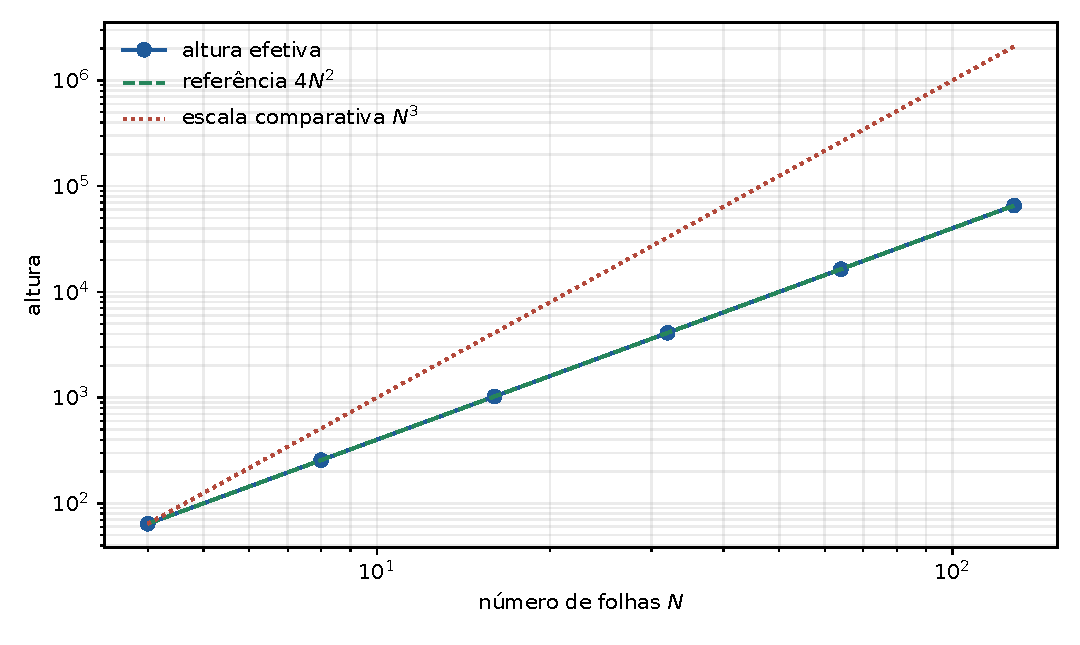
\includegraphics[width=.88\linewidth]{figuras/artigo_3/fig_altura_agendas.pdf}
 \caption{A altura efetiva da construção quadrática acompanha $N^2$; a
 curva $N^3$ corresponde ao fator de malha que o denominador comum absorve.}
 \label{artigo_3:fig:height-schedules}
\end{figure}

A \cref{artigo_3:fig:height-schedules} confirma, na construção quadrática auditada, a
separação entre a agenda provada $N^2$ e a escala comparativa $N^3$.

O programa \texttt{espacos\_aproximacao.py} usa
\texttt{fractions.Fraction} para reconstruir todos os valores nodais,
parâmetros, alturas e erros quadráticos. Ele verifica ainda, por enumeração
de $\mathcal Q_H$, a igualdade \eqref{artigo_3:eq:arithmetic-floor}; reproduz a
altura geométrica mínima $H=N$ das malhas uniformes em $[0,1]$; registra o
teste integral da série logarítmica; e emite o certificado simbólico da
\cref{artigo_3:prop:nonhomogeneous-functional}. Os testes são executados
independentemente da programação dinâmica das
seções de programação dinâmica do segundo artigo \citep{artigo_2-oliveiraII}.

\section{Reversibilidade regularizada e ponte quantitativa com redes ReLU}
\label{artigo_3:sec:regularized-reversibility}

Uma função linear por partes pode ser representada exatamente por uma rede ReLU
rasa por meio de uma expansão em hinges
\citep{artigo_2-devorehaninpetrova2021,artigo_1-daubechies2022}. Ela pode, portanto, ter poucas
folhas e, por isso, ter erro bruto nulo em todas as escalas posteriores sem
ganhar suavidade clássica. Essa barreira determina a forma dos teoremas
inversos desta seção.

Há três respostas, em níveis diferentes. Primeiro, o erro bruto admite uma
imersão inversa com perda, desde que se controle a inclinação efetivamente
realizada pelos aproximantes. Segundo, uma extensão marcada da biblioteca
remove a obstrução das regiões planas e dá uma equivalência exata com redes
ReLU rasas racionais de quebras diádicas; redes reais genéricas admitem uma
volta aproximada com recursos explícitos. Terceiro, usa-se um funcional de
realização, no sentido clássico de \citet{artigo_2-hristovivanov1990}, que soma ao erro
a autorregularidade do próprio aproximante. Nesse terceiro nível, a
desigualdade inversa é universal; a contribuição específica da biblioteca é o
lado direto de Jackson sob uma agenda explícita de altura racional.

A necessidade de orçar o crescimento dos coeficientes e a profundidade em
espaços de aproximação neural é enfatizada em
\citet{artigo_2-gribonval2022,artigo_2-grohs2023,artigo_1-guhring2021}. Em particular, o expoente crítico de Hölder
que surgirá no \cref{artigo_3:thm:raw-lossy-inverse} é a contraparte unidimensional e
uniforme do mecanismo de imersão de \citet{artigo_2-grohs2023}. As provas abaixo usam
apenas os módulos de suavidade e a altura da biblioteca.

\subsection{A obstrução que toda volta deve respeitar}

Escreva
\begin{equation}
 \psi(x)=\left|x-\frac12\right|,
 \qquad x\in[0,1].
 \label{artigo_3:eq:reverse-kink}
\end{equation}
Ela é uma montagem de duas folhas e altura $4$. Logo, para toda agenda que
eventualmente satisfaz $H(N)\ge4$,
\begin{equation}
 e_N^{\Library,H}(\psi)=0
 \quad\text{para todo $N$ suficientemente grande},
 \qquad
 \psi\in\mathscr A_q^\alpha(\Library,H)
 \quad(\alpha>0,\ 0<q\le\infty).
 \label{artigo_3:eq:kink-zero-raw-error}
\end{equation}
Por outro lado,
\begin{equation}
 \omega_2(\psi,h)_{\infty,[0,1]}=2h,
 \qquad 0<h\le\frac12,
 \label{artigo_3:eq:kink-exact-modulus-reverse}
\end{equation}
e, portanto,
\begin{equation}
 \psi\in B^s_{\infty,q}([0,1])
 \quad\Longleftrightarrow\quad
 s<1\ \text{ ou }\ (s=1\text{ e }q=\infty),
 \qquad 0<s<2.
 \label{artigo_3:eq:kink-besov-reverse}
\end{equation}
Com efeito, o salto de inclinação de $\psi$ é $2$, logo toda segunda diferença
de passo $h$ tem módulo no máximo $2h$; nos pontos
$1/2-h,1/2,1/2+h$ ela tem módulo exatamente $2h$. Substituir essa identidade
na caracterização diádica \eqref{artigo_3:eq:dyadic-besov-norm} prova
\eqref{artigo_3:eq:kink-besov-reverse}. Em particular, nenhum
teorema da forma
\begin{equation}
 e_N(f)=O(N^{-\alpha})\quad\Longrightarrow\quad
 f\in B^s_{\infty,q},
 \qquad s>1,
 \label{artigo_3:eq:forbidden-unregularized-converse}
\end{equation}
pode valer para o erro bruto do catálogo. Uma versão reversível deve conservar
informação sobre as quinas do aproximante, e não apenas sobre a distância de
$f$ a ele.

\subsection{A extensão marcada e a volta ReLU exata}

A inclinação nula foi
excluída da biblioteca original porque a imagem de um segmento constante não
recupera o suporte. Para estudar a volta, introduzimos uma extensão auxiliar
que guarda esse suporte como parte do código.

% MAPA artigo_3:5.1
\begin{definition}[biblioteca marcada completa]\label{map:artigo_3:5.1}
\label{artigo_3:def:marked-completion}
A biblioteca $\Library^\square$ é formada pelas quádruplas marcadas
\begin{equation}
 (k,m,y_0,s)\in\Nzero\times\mathbb Z\times\mathbb Q\times\mathbb Q,
 \label{artigo_3:eq:marked-atoms}
\end{equation}
com o mesmo segmento \eqref{artigo_3:eq:inherited-atom} e a mesma altura
\eqref{artigo_3:eq:inherited-height}. A marca $(k,m)$ é conservada na decodificação,
inclusive quando $s=0$. Denote por $\Aclass^\square(K)$ suas montagens
contínuas e por $\Aclass^\square_{N,H}(K)$ aquelas com no máximo $N$
folhas e altura atômica no máximo $H$.
\end{definition}

Tem-se $\Library\subset\Library^\square$. Para $s\ne0$, a marca é redundante
e a recuperação pela imagem coincide com a de $\Library$; para $s=0$, o
suporte é conservado explicitamente no par $(k,m)$.

Considere a forma ReLU reduzida
\begin{equation}
 R(x)=c+qx+\sum_{j=1}^{M}a_j\rho(x-\tau_j),
 \qquad 0<\tau_1<\cdots<\tau_M<1,
 \qquad a_j\ne0,
 \label{artigo_3:eq:reduced-relu-reverse}
\end{equation}
e suas inclinações locais
\begin{equation}
 \sigma_i=q+\sum_{j=1}^{i}a_j,
 \qquad 0\le i\le M.
 \label{artigo_3:eq:reverse-local-slopes}
\end{equation}
Para um conjunto finito $S\subset\mathbb D\cap(0,1)$, seja
$\mathcal T(S)$ a árvore diádica menos refinada cujas folhas não contêm
pontos de $S$ no interior. Ela é obtida subdividindo exatamente os ancestrais
necessários para transformar cada ponto de $S$ em fronteira.

% MAPA artigo_3:5.2
\begin{theorem}[reversibilidade rasa exata]\label{map:artigo_3:5.2}
\label{artigo_3:thm:exact-marked-reversal}
Uma função na forma reduzida \eqref{artigo_3:eq:reduced-relu-reverse} pertence a
$\Aclass^\square([0,1])$ se e somente se
\begin{equation}
 c,q,a_1,\ldots,a_M\in\mathbb Q,
 \qquad
 \tau_1,\ldots,\tau_M\in\mathbb D.
 \label{artigo_3:eq:marked-reversal-conditions}
\end{equation}
Nessas condições, $\mathcal T(\{\tau_1,\ldots,\tau_M\})$ é a única árvore
menos refinada que realiza $R$. Se $N_{\rm can}(R)$ é seu número de folhas e
$d_j$ é a profundidade diádica reduzida de $\tau_j$, então
\begin{equation}
 M+1\le N_{\rm can}(R)
 \le 1+\sum_{j=1}^{M}d_j.
 \label{artigo_3:eq:canonical-tree-leaf-bounds}
\end{equation}
A função pertence à biblioteca original $\Aclass([0,1])$ exatamente quando,
além de \eqref{artigo_3:eq:marked-reversal-conditions},
\begin{equation}
 \sigma_i\ne0\qquad(0\le i\le M).
 \label{artigo_3:eq:original-nonflat-condition}
\end{equation}
\end{theorem}

\begin{proof}
Suponha \eqref{artigo_3:eq:marked-reversal-conditions}. A árvore canônica transforma
todas as quebras em fronteiras. Em cada folha $J$, a função $R$ é afim, sua
inclinação é uma das $\sigma_i\in\mathbb Q$ e seu valor no centro é racional.
Esses dados determinam um átomo marcado; a continuidade de $R$ cola as peças.

Reciprocamente, toda montagem marcada é racional e afim no interior de cada
folha. Toda quebra real está em uma fronteira diádica, seu valor em $0$, a
inclinação inicial e os saltos de inclinação são racionais. Pela unicidade da
forma reduzida, obtém-se \eqref{artigo_3:eq:marked-reversal-conditions}.

Qualquer árvore que realize $R$ deve separar suas $M$ quebras reais, logo tem
ao menos $M+1$ folhas e refina $\mathcal T(S)$. Para inserir uma quebra de
profundidade $d_j$, bastam no máximo $d_j$ subdivisões novas. Como cada
subdivisão acrescenta uma folha, resulta a cota superior em
\eqref{artigo_3:eq:canonical-tree-leaf-bounds}. Finalmente, um átomo da biblioteca
original possui inclinação não nula; a condição é também suficiente folha a
folha.
\end{proof}

O teorema distingue duas contagens que coincidem apenas em partições já
alinhadas. $M+1$ conta regiões afins máximas; $N_{\rm can}$ conta células
diádicas. Por exemplo, uma única quebra em $1/4$ produz duas regiões, mas a
região $[1/4,1]$ precisa de duas folhas diádicas.

% MAPA artigo_3:5.3
\begin{definition}[altura canônica de rede]\label{map:artigo_3:5.3}
\label{artigo_3:def:canonical-network-height}
Para uma rede que satisfaz \eqref{artigo_3:eq:marked-reversal-conditions}, defina
\begin{equation}
 H_{\rm can}(R)=
 \max_{J_{k,m}\in\operatorname{leaf}(\mathcal T(S))}
 \max\{2,k+1,|m|+1,\height(R(x_{k,m})),\height(R'|_{J_{k,m}})\}.
 \label{artigo_3:eq:canonical-network-height}
\end{equation}
\end{definition}

Por construção, $H_{\rm can}(R)$ é exatamente a maior altura dos átomos na
montagem canônica. Essa é a medida que torna a ida e a volta isométricas no
recurso aritmético. A altura ingênua dos coeficientes
$(c,q,a_1,\ldots,a_M)$ não tem essa propriedade: somas de racionais podem
multiplicar denominadores.

% MAPA artigo_3:5.4
\begin{proposition}[forma ancorada e comprimento estrutural]\label{map:artigo_3:5.4}
\label{artigo_3:prop:anchored-relu-code}
Se $g\in\Aclass^\square_{N,H}([0,1])$, sua forma reduzida possui
$M\le N-1$ hinges e pode ser escrita, tomando o centro $x_*$ da folha mais à
esquerda, como
\begin{equation}
 g(x)=g(x_*)+\sigma_0(x-x_*)
      +\sum_{j=1}^{M}(\sigma_j-\sigma_{j-1})\rho(x-\tau_j).
 \label{artigo_3:eq:anchored-relu-form}
\end{equation}
Os valores $g(x_*)$ e $\sigma_i$ têm altura no máximo $H$, os saltos têm
altura no máximo $2H^2$, e os pontos diádicos são transmitidos por seus pares
estruturais. Consequentemente, existe uma codificação prefix-free da forma
ancorada com
\begin{equation}
 L_{\rm ReLU}^{\rm anc}(g)=O(N\log(2H)).
 \label{artigo_3:eq:anchored-network-bits}
\end{equation}

Na direção contrária, se os coeficientes de
\eqref{artigo_3:eq:reduced-relu-reverse} têm altura no máximo $W$ e as quebras têm
profundidade no máximo $D$ (e as quebras são diádicas em $(0,1)$), então
\begin{equation}
 H_{\rm can}(R)\le 2^{D+1}\,(M+2)\,W^{M+3},
 \qquad
 \log_2 H_{\rm can}(R)
 \le 5\bigl[(M+1)\log_2(2W)+D+\log_2(M+1)\bigr].
 \label{artigo_3:eq:reverse-height-bit-bound}
\end{equation}
\end{proposition}

\begin{proof}
Na ida, cada salto é a diferença de duas inclinações de altura no máximo
$H$, logo sua altura não excede $2H^2$. A altura atômica limita os inteiros
estruturais da célula, e todos os campos usam $O(\log(2H))$ bits. Somar os
$O(N)$ campos prova \eqref{artigo_3:eq:anchored-network-bits}, com constante explícita:
o código formalizado usa no máximo $40\,N\lfloor\log_2(2H)\rfloor$ bits. O ancoramento evita
expandir desnecessariamente $g(x_*)-\sigma_0x_*$ em um intercepto com
denominador diádico explícito.

Na volta, toda folha $J_{k,m}$ de $\mathcal T(S)$ tem $k\le D$ e
$|m|+1\le 2^k\le 2^D$. Cada inclinação local $\sigma_i$ é soma de no máximo $M+1$
racionais de altura $\le W$: um denominador comum é $\le W^{M+1}$ e
$|\sigma_i|\le(M+1)W$, logo $\operatorname{ht}\sigma_i\le (M+1)W^{M+2}$. O centro
$x_{k,m}=(2m+1)/2^{k+1}$ e as quebras têm denominador dividindo $2^{D+1}$, e
$0\le \max\{0,x_{k,m}-\tau_j\}\le1$. Assim, $R(x_{k,m})=c+qx_{k,m}+\sum_j
a_j\max\{0,x_{k,m}-\tau_j\}$ admite o denominador comum
$\operatorname{den}(c)\operatorname{den}(q)\,2^{D+1}\prod_j\operatorname{den}(a_j)\le
2^{D+1}W^{M+2}$ (a parte diádica é compartilhada por todas as parcelas) e módulo
$\le (M+2)W$; portanto $\operatorname{ht}R(x_{k,m})\le 2^{D+1}(M+2)W^{M+3}$. Os
demais termos de \eqref{artigo_3:eq:canonical-network-height} ($2$, $k+1\le D+1$,
$|m|+1\le 2^D$) são menores, o que dá $H_{\rm can}(R)\le 2^{D+1}(M+2)W^{M+3}$.
Tomando $\log_2$, e usando $W\ge1$, $\log_2(M+2)\le 1+\log_2(M+1)$ e
$(M+1)\log_2(2W)\ge1$, obtém-se
\[
 \log_2 H_{\rm can}\le D+1+\bigl(1+\log_2(M+1)\bigr)+(M+3)\log_2 W
 \le 5\bigl[(M+1)\log_2(2W)+D+\log_2(M+1)\bigr].
\]
\end{proof}

\begin{observacaoSN}\label{artigo_3:rem:reverse-height-correction}
O fator é $M+1$, e não $M$, no primeiro termo: há $M+1$ inclinações locais e
cada uma é soma de até $M+1$ racionais. A versão com $M\log(2W)$ é falsa já para
$M=0$: em $R(x)=x$ ($M=0$, $D=0$, $W=1$) tem-se $H_{\rm can}=2$, de modo que
$\log_2 H_{\rm can}=1$ e o lado direito é $0$; e em $R(x)=Wx$ tem-se
$H_{\rm can}\ge W$ (a altura da inclinação), de modo que nenhum termo constante
repara a cota. A volta corrigida está formalizada em
\texttt{Pendencias/AlturaInversa.lean}; a ida (forma ancorada e código prefix-free)
está formalizada em \texttt{Pendencias/FormaAncorada.lean} e
\texttt{Pendencias/CodigoAncorado.lean}.
\end{observacaoSN}

Assim, a reversibilidade exata preserva comprimento binário em ordem
polinomial, mas não preserva a altura ingênua coeficiente a coeficiente. A
altura correta do lado neural é \eqref{artigo_3:eq:canonical-network-height}, isto é,
o recurso aritmético depois da função ser colocada em sua partição diádica
canônica.

\subsection{Volta aproximada para redes rasas reais}

Quebras não diádicas e coeficientes irracionais impedem igualdade exata, mas
não uma conversão quantitativa. Cotas de erro e de recursos para aproximação
ReLU, inclusive sob restrições de codificação, são estudadas em
\citet{artigo_1-yarotsky2017,artigo_1-bolcskei2019}. A próxima estimativa dá uma forma explícita
da densidade compatível com a biblioteca.

% MAPA artigo_3:5.5
\begin{theorem}[reversão aproximada quantizada]\label{map:artigo_3:5.5}
\label{artigo_3:thm:quantized-approximate-reverse}
Seja $R$ como em \eqref{artigo_3:eq:reduced-relu-reverse}, agora com parâmetros reais,
e suponha
\begin{equation}
 |c|,|q|,|a_1|,\ldots,|a_M|\le W,
 \qquad W\ge1.
 \label{artigo_3:eq:real-network-weight-bound}
\end{equation}
Para todo $0<\varepsilon\le1$, existe uma montagem da biblioteca original
$g_\varepsilon\in\Aclass([0,1])$ tal que
\begin{align}
 \|R-g_\varepsilon\|_\infty&\le\varepsilon,
 \label{artigo_3:eq:approximate-reverse-error}\\
 |\Lambda(g_\varepsilon)|&\le1+MD_\varepsilon,
 \qquad
 D_\varepsilon=
 \left\lceil\log_2\frac{C(M+1)(W+1)}{\varepsilon}\right\rceil,
 \label{artigo_3:eq:approximate-reverse-leaves}\\
 \height_{\max}(g_\varepsilon)
 &\le
 C(M+1)^3(W+1)^3\varepsilon^{-2},
 \label{artigo_3:eq:approximate-reverse-height}
\end{align}
onde $C$ é universal. A conclusão permanece válida quando $R$ possui regiões
planas.
\end{theorem}

\begin{proof}
Ponha
\[
 \delta=\frac{\varepsilon}{16(M+1)(W+1)}.
\]
Escolha um denominador comum $Q\asymp\delta^{-1}$ e aproxime
$c,q,a_1,\ldots,a_M$ por múltiplos de $1/Q$ com erro no máximo $\delta$.
Aproxime cada $\tau_j$ por um diádico de profundidade
$D\le D_\varepsilon$. A função $z\mapsto\rho(x-z)$ é $1$-Lipschitz e
$0\le\rho(x-z)\le1$ em $[0,1]$, de modo que a soma dos erros de coeficientes
e deslocamentos é no máximo
\[
 (M+2)\delta+M(W+\delta)\delta.
\]
Nós que colidem são combinados; nós que chegam a $0$ são absorvidos no termo
linear e os que chegam a $1$ desaparecem no domínio.

Resta impedir inclinações locais nulas. Depois da quantização há no máximo
$M+1$ valores proibidos para uma perturbação global da inclinação. Entre
$M+2$ múltiplos positivos consecutivos de $1/Q$, escolha um que não seja
proibido e acrescente o termo correspondente $\eta x$. A escolha de $Q$ e a
folga em $\delta$ mantêm o erro total abaixo de $\varepsilon$.

A árvore canônica exige no máximo $1+MD$ folhas pelo
\cref{artigo_3:thm:exact-marked-reversal}. Inclinações locais têm denominador comum
$Q$ e numeradores $O((M+1)(W+1)Q)$. Valores nos centros têm denominador que
divide $Q2^{D+1}$ e numeradores
$O((M+1)(W+1)Q2^D)$. Como
$Q,2^D=O((M+1)(W+1)\varepsilon^{-1})$, segue
\eqref{artigo_3:eq:approximate-reverse-height}. A perturbação final permite usar a
biblioteca original, não apenas sua extensão marcada.
\end{proof}

% MAPA artigo_3:5.6
\begin{corollary}[redes profundas medidas pela função realizada]\label{map:artigo_3:5.6}
\label{artigo_3:cor:deep-functional-reverse}
Se uma rede ReLU univariada arbitrária realiza uma função $F$ com $R(F)$
regiões afins máximas, norma uniforme no máximo $B$ e constante de Lipschitz
no máximo $L_F$, então o \cref{artigo_3:thm:quantized-approximate-reverse} vale com
\begin{equation}
 M=R(F)-1,
 \qquad
 W\le2\max\{1,B,L_F\}.
 \label{artigo_3:eq:deep-realized-resources}
\end{equation}
\end{corollary}

\begin{proof}
Toda função ReLU univariada é linear por partes e admite a forma hinge rasa
canônica, independentemente da arquitetura que a produziu. A inclinação
inicial tem módulo no máximo $L_F$, cada salto tem módulo no máximo $2L_F$ e
$|F(0)|\le B$. Aplique o teorema anterior.
\end{proof}

A relação entre profundidade e número de regiões pode ser exponencial, como nas
construções de separação por profundidade de \citet{artigo_2-telgarsky2016}. Para o bloco
tenda
\[
 T(x)=2\rho(x)-4\rho(x-\tfrac12),\qquad x\in[0,1],
\]
a iterada $T_L=T^{\circ L}$ possui exatamente $2^L$ regiões afins máximas,
com inclinações $\pm2^L$: cada composição bissecta todas as regiões do nível
anterior. Assim, toda montagem que realize $T_L$ exatamente requer ao menos
$2^L$ folhas e altura atômica ao menos $2^L$. A dependência do corolário nos
recursos realizados conserva, portanto, essa separação exponencial.

A \cref{artigo_3:tab:deep-tent-network} explicita os primeiros oito níveis dessa lei,
e a \cref{artigo_3:fig:network-restrictions} contrasta número de blocos, regiões
realizadas e recursos mínimos da biblioteca.

\begin{table}[t]
 \centering
 \small
 \begin{tabular}{rrrr}
\toprule
profundidade $L$ & blocos & regiões/folhas mín. & altura mín.\\
\midrule
1 & 1 & 2 & 2\\
2 & 2 & 4 & 4\\
3 & 3 & 8 & 8\\
4 & 4 & 16 & 16\\
5 & 5 & 32 & 32\\
6 & 6 & 64 & 64\\
7 & 7 & 128 & 128\\
8 & 8 & 256 & 256\\
\bottomrule
\end{tabular}

 \caption{Separação exata para a tenda iterada: $L$ blocos produzem $2^L$
 regiões, e qualquer montagem exata requer ao menos $2^L$ folhas e altura
 atômica ao menos $2^L$.}
 \label{artigo_3:tab:deep-tent-network}
\end{table}

\begin{figure}[t]
 \centering
 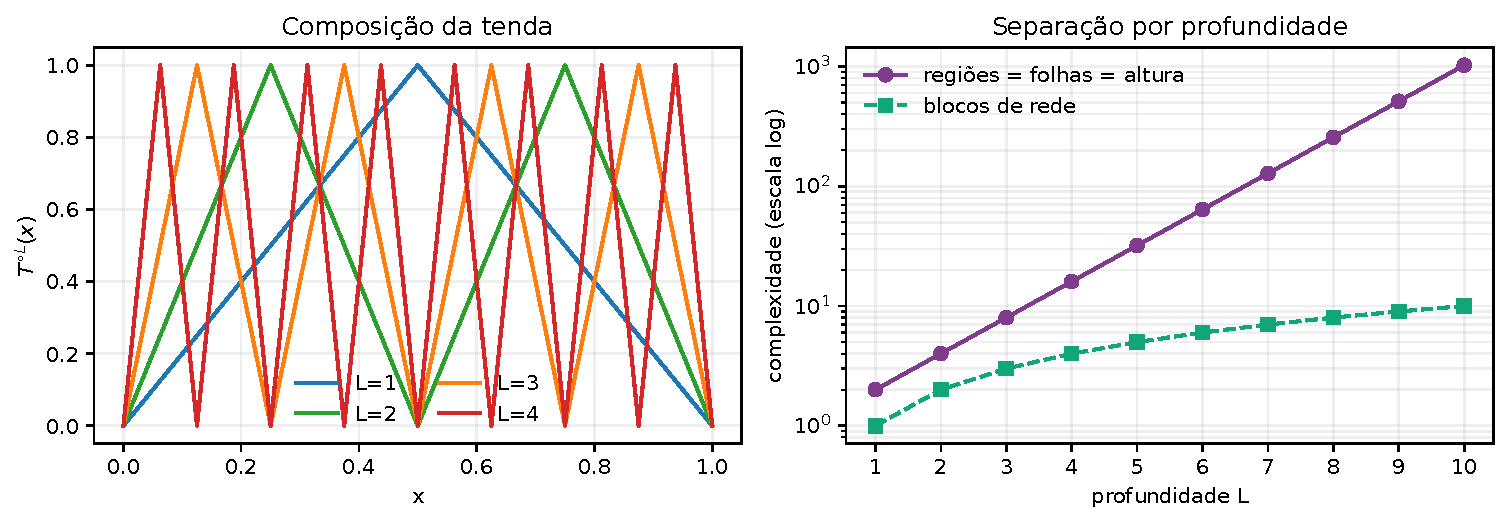
\includegraphics[width=.88\linewidth]{figuras/artigo_3/fig_restricoes_rede.pdf}
 \caption{Crescimento dos recursos realizados pela tenda iterada. Os pontos
 provêm de identidades exatas; as linhas apenas guiam a leitura.}
 \label{artigo_3:fig:network-restrictions}
\end{figure}

\begin{table}[t]
 \centering
 \small
 \begin{tabular}{rrrrrr}
\toprule
$M$ & $\varepsilon$ & $D$ & folhas & cota de folhas & erro/$\varepsilon$\\
\midrule
1 & $1/32$ & 12 & 13 & 13 & 0.0099\\
1 & $1/64$ & 13 & 14 & 14 & 0.0037\\
1 & $1/128$ & 14 & 15 & 15 & 0.0131\\
1 & $1/32$ & 11 & 12 & 12 & 0.0245\\
1 & $1/64$ & 12 & 13 & 13 & 0.0099\\
1 & $1/128$ & 13 & 14 & 14 & 0.0120\\
\bottomrule
\end{tabular}

 \caption{Auditoria racional da reversão aproximada. As redes de entrada
 possuem quebras não diádicas. O erro é calculado exatamente no conjunto
 unido de quebras, onde o máximo de uma diferença linear por partes é
 atingido.}
 \label{artigo_3:tab:approximate-reverse-audit}
\end{table}

Os casos quantizados da \cref{artigo_3:tab:approximate-reverse-audit} verificam, com
frações exatas, a cota de erro e a permanência na biblioteca original.

\subsection{A melhor recíproca para o erro bruto}

Todo $g\in\Sigma_N^{\Library,H}$ é $H(N)$-Lipschitz, pois em cada folha sua
inclinação $s$ satisfaz $|s|\le\height(s)\le H(N)$. Consequentemente,
$\omega_2(g,t)_\infty\le2H(N)t$. Essa desigualdade de tipo Bernstein contém
uma recíproca verdadeira, desde que se aceite a perda imposta pelo crescimento
das inclinações. A formulação seguinte não depende da aritmética.

% MAPA artigo_3:5.7
\begin{theorem}[imersão inversa sob crescimento de Lipschitz]\label{map:artigo_3:5.7}
\label{artigo_3:thm:raw-lossy-inverse}
Sejam $\mathcal G_N\subset C([0,1])$ famílias de aproximantes tais que
\begin{equation}
 \operatorname{Lip}(g)\le C_LN^\gamma
 \qquad(g\in\mathcal G_N),
 \qquad \gamma\ge0,
 \label{artigo_3:eq:lipschitz-growth-family}
\end{equation}
e defina
$e_N^{\mathcal G}(f)=\inf_{g\in\mathcal G_N}\|f-g\|_\infty$. Se
\begin{equation}
 A_\alpha(f):=\sup_{N\ge1}N^\alpha e_N^{\mathcal G}(f)<\infty,
 \qquad \alpha>0,
 \label{artigo_3:eq:raw-rate-assumption}
\end{equation}
então, com
\begin{equation}
 \theta_* = \frac{\alpha}{\alpha+\gamma},
 \label{artigo_3:eq:critical-reverse-exponent}
\end{equation}
vale
\begin{equation}
 \omega_2(f,t)_\infty
 \le C_{\alpha,\gamma}(A_\alpha(f)+C_L)t^{\theta_*},
 \qquad 0<t\le\frac12.
 \label{artigo_3:eq:raw-inverse-modulus}
\end{equation}
Consequentemente,
\begin{equation}
 f\in B^{\theta_*}_{\infty,\infty}([0,1])
 \quad\text{e}\quad
 f\in B^\theta_{\infty,r}([0,1])
 \quad(0<\theta<\theta_*,\ 0<r\le\infty).
 \label{artigo_3:eq:raw-inverse-besov}
\end{equation}
\end{theorem}

\begin{proof}
Para qualquer $g\in\mathcal G_N$, a desigualdade triangular para segundas
diferenças e a propriedade Lipschitz dão
\begin{equation}
 \omega_2(f,t)_\infty
 \le4\|f-g\|_\infty+2C_LN^\gamma t.
 \label{artigo_3:eq:inverse-balance}
\end{equation}
Escolha $N$ comparável a $t^{-1/(\alpha+\gamma)}$ e use um aproximante
arbitrariamente próximo do ínfimo. Os dois termos do lado direito passam a
ser $O(t^{\alpha/(\alpha+\gamma)})$, o que prova
\eqref{artigo_3:eq:raw-inverse-modulus}. A caracterização diádica de Besov fornece o
endpoint por supremo. Para $\theta<\theta_*$, a sequência normalizada ganha o
fator geométrico $2^{-j(\theta_*-\theta)}$ e pertence a todo $\ell^r$.
\end{proof}

% MAPA artigo_3:5.8
\begin{corollary}[aplicação às agendas diretas]\label{map:artigo_3:5.8}
\label{artigo_3:cor:raw-library-inverse}
Se $H(N)\le C N^\gamma$, então
\begin{equation}
 \mathscr A_q^\alpha(\Library,H)
 \subset B^{\alpha/(\alpha+\gamma)}_{\infty,\infty}([0,1]),
 \qquad 0<q\le\infty.
 \label{artigo_3:eq:raw-library-inverse}
\end{equation}
Para as agendas $H_{s,0}$ da \cref{artigo_3:sec:direct-height}, isso dá
\begin{equation}
 \mathscr A_q^s(\Library,H_{s,0})
 \subset B^{\vartheta_s}_{\infty,\infty},
 \qquad
 \vartheta_s=
 \begin{cases}
 s/(s+1),&0<s<1,\\
 1/2,&1\le s<2.
 \end{cases}
 \label{artigo_3:eq:corrected-schedule-raw-inverse}
\end{equation}
Se a agenda possui ainda um fator logarítmico, a mesma conclusão vale para
toda ordem estritamente menor que $\vartheta_s$.
\end{corollary}

\begin{proof}
Todo elemento de $\Sigma_N^{\Library,H}$ é $H(N)$-Lipschitz. O funcional com
$q<\infty$ controla o de supremo pela redução diádica do
\cref{artigo_3:thm:dyadic-rate-equivalence}. Um fator logarítmico é dominado por
$N^\eta$ para qualquer $\eta>0$; aplique o teorema com
$\gamma+\eta$ e faça $\eta\downarrow0$.
\end{proof}

O \cref{artigo_3:thm:critical-tent-comb} realiza o expoente \eqref{artigo_3:eq:critical-reverse-exponent} na biblioteca original, com inclinações locais não nulas, na faixa $0<\alpha\le\gamma$.

% MAPA artigo_3:5.9
\begin{theorem}[agudeza por um pente de tendas]\label{map:artigo_3:5.9}
\label{artigo_3:thm:critical-tent-comb}
Fixe $0<\alpha\le\gamma$ e ponha
$\theta_*=\alpha/(\alpha+\gamma)$. Existe
$f\in C([0,1])$ e uma constante $C$ tais que, para a biblioteca original sob
$H(N)=\lceil CN^\gamma\rceil$,
\begin{equation}
 e_N^{\Library,H}(f)\le CN^{-\alpha},
 \label{artigo_3:eq:comb-approximation-rate}
\end{equation}
mas
\begin{equation}
 f\notin B^\theta_{\infty,\infty}\quad(\theta>\theta_*),
 \qquad
 f\notin B^{\theta_*}_{\infty,r}\quad(0<r<\infty).
 \label{artigo_3:eq:comb-sharpness}
\end{equation}
\end{theorem}

\begin{proof}
Escolha um inteiro $J_0$ tão grande que
$J_0(\alpha+\gamma)>3$. Para $j\ge1$, ponha
\[
 a_j=\lceil J_0\alpha j\rceil,
 \qquad b_j=\lfloor J_0\gamma j\rfloor,
 \qquad r_j=a_j+b_j-1.
\]
No intervalo diádico $J_{r_j,1}$, coloque uma tenda $\phi_j$ de altura
$2^{-a_j}$, nula nas extremidades e linear em cada metade. As escolhas
garantem que os suportes são disjuntos e acumulam apenas em $0$. Defina
$f=\sum_{j\ge1}\phi_j$.

A inclinação da $j$-ésima tenda tem módulo $2^{b_j}$ e os valores centrais de
suas duas metades têm altura $2^{a_j+1}$. Seja $T_j$ a árvore diádica em pente
que isola as duas metades das primeiras $j$ tendas. Ela possui
$O(r_j+j)$ folhas; fora dessas tendas, a soma parcial
$f_j=\sum_{i\le j}\phi_i$ é nula em cada folha restante.

Para eliminar todas as inclinações nulas sem alterar o alvo $f$, subdivida uma
vez cada folha plana $J$ de $T_j$ e, sobre $J$, acrescente uma tenda
$\psi_{J,j}$ nula nos extremos e de altura
\[
 \delta_j=2^{-a_{j+1}-2}
\]
no ponto médio. Os suportes dessas pequenas tendas são disjuntos. A função
\[
 g_j=f_j+\sum_{J\ {\rm plano\ em}\ T_j}\psi_{J,j}
\]
é contínua e tem inclinação não nula em toda folha da árvore refinada. Logo
$g_j$ é uma montagem da biblioteca original, não da extensão marcada.

Resta conferir os dois orçamentos. A árvore refinada tem ainda
$O(r_j+j)$ folhas. Em uma folha plana de profundidade $d\le r_j+1$, a nova
inclinação tem módulo $2^{d+1}\delta_j$; sua altura é limitada por
\[
 \max\{2^{a_{j+1}+1},\,2^{r_j-a_{j+1}}\}
 \le C2^{J_0\gamma j}.
\]
Os valores centrais novos têm altura no máximo $2^{a_{j+1}+3}$, e os
parâmetros das tendas originais são limitados por
$C\max\{2^{a_j},2^{b_j}\}$. As células profundas do pente têm índices
$m\in\{0,1,2,3\}$; portanto escala e translação obedecem à mesma cota.
Como $\alpha\le\gamma$, todos esses termos são no máximo
$CN_j^\gamma$ para $N_j=2^{J_0j}$, depois de aumentar $C$. Também
$O(r_j+j)\le N_j$ para $j$ grande; as finitíssimas escalas iniciais são
absorvidas em $C$ e por uma reindexação finita.

Por disjunção dos suportes,
\[
 \|f-g_j\|_\infty
 \le \Bigl\|\sum_{i>j}\phi_i\Bigr\|_\infty+\delta_j
 \le 2^{-a_{j+1}}+\delta_j
 \le C N_j^{-\alpha}.
\]
Para $N_j\le N<N_{j+1}$, use $g_j$; a razão
$N_{j+1}/N_j=2^{J_0}$ é fixa. A monotonicidade da agenda e o ajuste dessa
constante provam \eqref{artigo_3:eq:comb-approximation-rate} para todo $N$.

Se $h_j=2^{-(r_j+1)}$ é a meia-largura da tenda, os valores
$0,2^{-a_j},0$ dão
\[
 \omega_2(f,h_j)_\infty\ge2^{1-a_j}\asymp h_j^{\theta_*}.
\]
Isso exclui toda ordem maior no supremo e torna constante uma subsequência do
coeficiente crítico, que não pertence a nenhum $\ell^r$ finito.
\end{proof}

A exigência $\alpha\le\gamma$ cobre em particular as agendas críticas da
\cref{artigo_3:sec:direct-height}. Ela também expõe por que a informação correta é a inclinação
realizada, não a altura do endereço isoladamente.

\subsection{Funcional de realização: lado direto com altura controlada}

A agudeza do teorema anterior fixa a regularidade determinada pelo erro bruto
e por uma cota de Lipschitz. Para comparar com a suavidade clássica, considere
o funcional de realização associado ao módulo de segunda ordem. Funcionais
desse tipo foram introduzidos para substituir $K$-funcionais degenerados em
aproximação restrita \citep{artigo_2-hristovivanov1990}. Para $N\ge2$, defina
\begin{equation}
 \mathcal R_N^{\Library,H}(f)
 :=\inf_{g\in\Sigma_N^{\Library,H}([0,1])}
 \left\{\|f-g\|_\infty+
 \omega_2(g,N^{-1})_\infty\right\}.
 \label{artigo_3:eq:self-roughness-certificate}
\end{equation}
O primeiro termo mede fidelidade; o segundo impede que uma função com quinas
receba suavidade apenas porque já pertence ao catálogo.

% MAPA artigo_3:5.10
\begin{lemma}[desigualdade inversa universal]\label{map:artigo_3:5.10}
\label{artigo_3:lem:universal-regularized-inverse}
Para toda agenda, toda $f\in C([0,1])$ e todo $N\ge2$,
\begin{equation}
 \frac14\omega_2(f,N^{-1})_\infty
 \le \mathcal R_N^{\Library,H}(f).
 \label{artigo_3:eq:universal-regularized-lower}
\end{equation}
\end{lemma}

\begin{proof}
Para qualquer $g$ admissível,
\[
 \omega_2(f,N^{-1})_\infty
 \le4\|f-g\|_\infty+\omega_2(g,N^{-1})_\infty
 \le4\bigl(\|f-g\|_\infty+\omega_2(g,N^{-1})_\infty\bigr).
\]
Tome o ínfimo.
\end{proof}

% MAPA artigo_3:5.11
\begin{remark}[o que o funcional mede]\label{map:artigo_3:5.11}
\label{artigo_3:rem:realization-functional-scope}
A cota inversa decorre da desigualdade triangular para segundas diferenças e vale para qualquer família de candidatos. O lado direto usa a biblioteca para construir aproximantes sob a agenda aritmética da \cref{artigo_3:sec:direct-height}.
\end{remark}

% MAPA artigo_3:5.12
\begin{theorem}[Jackson racional para o funcional de realização]\label{map:artigo_3:5.12}
\label{artigo_3:thm:regularized-jackson-bernstein}
Se $0<s<2$ e $f\in B^s_{\infty,\infty}([0,1])$, então, para toda potência de
dois $N$ suficientemente grande e toda altura que satisfaz as hipóteses do
\cref{artigo_3:lem:rational-jackson-height},
\begin{equation}
 \frac14\omega_2(f,N^{-1})_\infty
 \le \mathcal R_N^{\Library,H}(f)
 \le C_0\omega_2(f,N^{-1})_\infty+\frac{C_f}{H(N)},
 \label{artigo_3:eq:two-sided-regularized-equivalence}
\end{equation}
onde $C_0$ é universal e $C_f$ depende apenas de $\|f\|_\infty$ e das
constantes fixadas na racionalização.
Se $\|f\|_{B^s_{\infty,\infty}}^*\le B$, $B\ge1$, e
$H(N)\ge\widehat H_{s,0}^{[B]}(N)$, a mesma estimativa vale para toda potência
diádica $N\ge2$, com $C_f/H(N)$ substituído por $C(B+1)/H(N)$ e constantes
independentes de $f$.
\end{theorem}

\begin{proof}
A cota inferior é o lema anterior. Para a superior, tome o aproximante
racional $g_{N,H}$ do \cref{artigo_3:lem:rational-jackson-height}. Ele satisfaz
\[
 \|f-g_{N,H}\|_\infty
 \le2C_W\omega_2(f,N^{-1})_\infty+C_fH(N)^{-1}.
\]
Além disso, a desigualdade triangular aplicada na direção contrária dá
\[
 \omega_2(g_{N,H},N^{-1})_\infty
 \le\omega_2(f,N^{-1})_\infty+4\|f-g_{N,H}\|_\infty.
\]
Somar as duas estimativas e usar $g_{N,H}$ na definição de
$\mathcal R_N$ prova a cota superior. Na versão sobre a bola, aplique a parte
uniforme do mesmo lema; ela substitui o termo de quantização por
$8(B+1)/H(N)$ em todas as escalas diádicas, e o mesmo cálculo apenas altera a
constante universal.
\end{proof}

Defina o estrato reversível
\begin{equation}
 \mathscr R_q^s(\Library,H)
 :=\left\{f\in C([0,1]):
 \left\|\bigl(2^{rs}\mathcal R_{2^r}^{\Library,H}(f)\bigr)_{r\ge1}
 \right\|_{\ell^q}<\infty\right\}.
 \label{artigo_3:eq:reversible-stratum}
\end{equation}

% MAPA artigo_3:5.13
\begin{theorem}[caracterização pelo funcional de realização]\label{map:artigo_3:5.13}
\label{artigo_3:thm:complete-besov-reversibility}
Para $0<s<2$, valem as igualdades de conjuntos
\begin{align}
 B^s_{\infty,\infty}([0,1])
 &=\mathscr R_\infty^s(\Library,H_{s,0}),
 \label{artigo_3:eq:complete-reverse-endpoint}\\
 B^s_{\infty,q}([0,1])
 &=\mathscr R_q^s(\Library,H_{s,0}),
 &&0<q<\infty,\quad0<s<1,
 \label{artigo_3:eq:complete-reverse-subcritical}\\
 B^s_{\infty,q}([0,1])
 &=\mathscr R_q^s(\Library,H_{s,\kappa}),
 &&0<q<\infty,\quad1\le s<2,\quad\kappa>1/q.
 \label{artigo_3:eq:complete-reverse-critical}
\end{align}
Pode-se substituir a agenda logarítmica da última linha por qualquer agenda
com folga polinomial \eqref{artigo_3:eq:polynomial-slack-schedule}.
\end{theorem}

\begin{proof}
Se o funcional em \eqref{artigo_3:eq:reversible-stratum} é finito, a desigualdade
universal do \cref{artigo_3:lem:universal-regularized-inverse}, na forma
\eqref{artigo_3:eq:universal-regularized-lower}, e a caracterização diádica
\eqref{artigo_3:eq:dyadic-besov-norm} dão imediatamente
$f\in B^s_{\infty,q}$.

Na direção direta, aplique a cota superior. O termo do módulo pertence a
$\ell^q$ pela definição de Besov. Para $s<1$,
\[
 \frac{N^s}{H_{s,0}(N)}=O(N^{s-1}),
\]
que é geometricamente somável nas potências de dois. Para $q=\infty$ e
$s\ge1$, $N^s/H_{s,0}(N)$ é limitado. Para $q<\infty$ e $s\ge1$, a agenda
logarítmica produz $(\log(eN))^{-\kappa}$, cuja subsequência diádica pertence
a $\ell^q$ exatamente sob $\kappa q>1$. A folga polinomial produz
$N^{-\eta}$. Um número finito de escalas iniciais não altera pertinência.
\end{proof}

O dado adicional que torna a taxa reversível é a segunda diferença do próprio
aproximante na escala pareada. A altura permanece aritmética e usa as agendas
da \cref{artigo_3:sec:direct-height}; a uniformidade quantitativa sobre bolas é dada
pelos \cref{artigo_3:thm:direct-besov-height,artigo_3:cor:uniform-besov-ball-embedding}. A caracterização refere-se ao funcional de realização.

Para a quina \eqref{artigo_3:eq:reverse-kink}, tomar $g=\psi$ zera o primeiro termo,
mas deixa
\begin{equation}
 \mathcal R_N^{\Library,H}(\psi)
 \le\omega_2(\psi,N^{-1})_\infty=\frac2N.
 \label{artigo_3:eq:kink-regularized-rate}
\end{equation}
A cota universal mostra a mesma ordem. Logo a taxa reversível é exatamente
um, em acordo com \eqref{artigo_3:eq:kink-besov-reverse}, e não infinita.

\begin{table}[t]
 \centering
 \small
 \begin{tabular}{rrrrr}
\toprule
$N$ & $e_N(\psi)$ & $\omega_2(\psi,N^{-1})$ & $N\omega_2$ & $N^{3/2}\omega_2$\\
\midrule
4 & 0 & $1/2$ & 2.000 & 4.000\\
8 & 0 & $1/4$ & 2.000 & 5.657\\
16 & 0 & $1/8$ & 2.000 & 8.000\\
32 & 0 & $1/16$ & 2.000 & 11.314\\
64 & 0 & $1/32$ & 2.000 & 16.000\\
128 & 0 & $1/64$ & 2.000 & 22.627\\
\bottomrule
\end{tabular}

 \caption{A quina sob o erro bruto e a parcela de autorregularidade obtida
 com o candidato $g=\psi$. Embora $e_N(\psi)=0$, essa parcela é $2/N$; a
 cota universal \eqref{artigo_3:eq:universal-regularized-lower} garante que o ínfimo
 completo tem a mesma ordem $N^{-1}$.}
 \label{artigo_3:tab:kink-regularized-certificate}
\end{table}

A \cref{artigo_3:tab:kink-regularized-certificate} torna explícita a diferença entre
erro bruto nulo e autorregularidade de ordem $N^{-1}$.

\subsection{Estabilidade da caracterização ao ampliar a arquitetura}

O certificado é definido no espaço de funções, independentemente de uma
parametrização neural, o que permite comparar famílias arquiteturais inteiras.

% MAPA artigo_3:5.14
\begin{theorem}[reversibilidade estável por inclusão de redes]\label{map:artigo_3:5.14}
\label{artigo_3:thm:architecture-stable-reversibility}
Seja $(\mathcal N_N)$ qualquer família de funções realizadas por redes ReLU
aninhada no orçamento, isto é,
\begin{equation}
 0\in\mathcal N_N,
 \qquad \mathcal N_N\subseteq\mathcal N_{N+1}
 \qquad(N\ge1),
 \label{artigo_3:eq:network-family-nesting}
\end{equation}
e suponha que, para alguma constante $c\ge1$,
\begin{equation}
 \Sigma_N^{\Library,H}([0,1])\subseteq\mathcal N_{\lceil cN\rceil}
 \qquad(N\ge1).
 \label{artigo_3:eq:network-family-contains-library}
\end{equation}
Defina
\begin{equation}
 \mathcal R_N^{\mathcal N}(f)
 =\inf_{R\in\mathcal N_N}
 \left\{\|f-R\|_\infty+\omega_2(R,N^{-1})_\infty\right\}.
 \label{artigo_3:eq:network-regularized-certificate}
\end{equation}
Sob cada uma das agendas do
\cref{artigo_3:thm:complete-besov-reversibility}, substituir
$\mathcal R_N^{\Library,H}$ por $\mathcal R_N^{\mathcal N}$ preserva as
igualdades \eqref{artigo_3:eq:complete-reverse-endpoint}--
\eqref{artigo_3:eq:complete-reverse-critical}.
\end{theorem}

\begin{proof}
A desigualdade inversa
\[
 \omega_2(f,N^{-1})_\infty\le4\mathcal R_N^{\mathcal N}(f)
\]
vale para toda função contínua $R$, independentemente da arquitetura. Essa é
a inclusão do estrato neural no Besov. Na direção direta, realize na família
neural o aproximante racional da
\cref{artigo_3:thm:regularized-jackson-bernstein}. Ponha
$d=2^{\lceil\log_2c\rceil}$. Para todo orçamento diádico $M=2^r\ge d$, o
número $n=M/d$ é também uma potência de dois e
$\lceil cn\rceil\le M$. Por \eqref{artigo_3:eq:network-family-contains-library} e pelo
aninhamento \eqref{artigo_3:eq:network-family-nesting},
\[
 \Sigma_n^{\Library,H}([0,1])
 \subseteq\mathcal N_{\lceil cn\rceil}
 \subseteq\mathcal N_M.
\]
Se $g_{n,H}$ é o aproximante usado naquele teorema, a monotonicidade do módulo
na escala fornece
\begin{align*}
 \mathcal R_M^{\mathcal N}(f)
 &\le \|f-g_{n,H}\|_\infty+\omega_2(g_{n,H},M^{-1})_\infty\\
 &\le \|f-g_{n,H}\|_\infty+\omega_2(g_{n,H},n^{-1})_\infty\\
 &\le C_0\omega_2(f,n^{-1})_\infty+\frac{C_f}{H(n)}.
\end{align*}
Como $M=dn$, multiplicar por $M^s$ introduz apenas o fator fixo $d^s$, e a
passagem de $M$ a $n$ desloca por $\log_2d$ índices as sequências diádicas.
As mesmas estimativas de $\ell^q$ da
\cref{artigo_3:thm:complete-besov-reversibility} concluem a direção direta. Um número
finito de escalas $M<d$ não afeta o estrato.
\end{proof}

Pelo \cref{artigo_3:thm:architecture-stable-reversibility}, ampliar a família de redes preserva a caracterização: a cota inferior depende do módulo do alvo. Redes profundas podem reduzir o erro, mas o certificado permanece maior ou igual a um quarto desse módulo.

\begin{figure}[t]
 \centering
 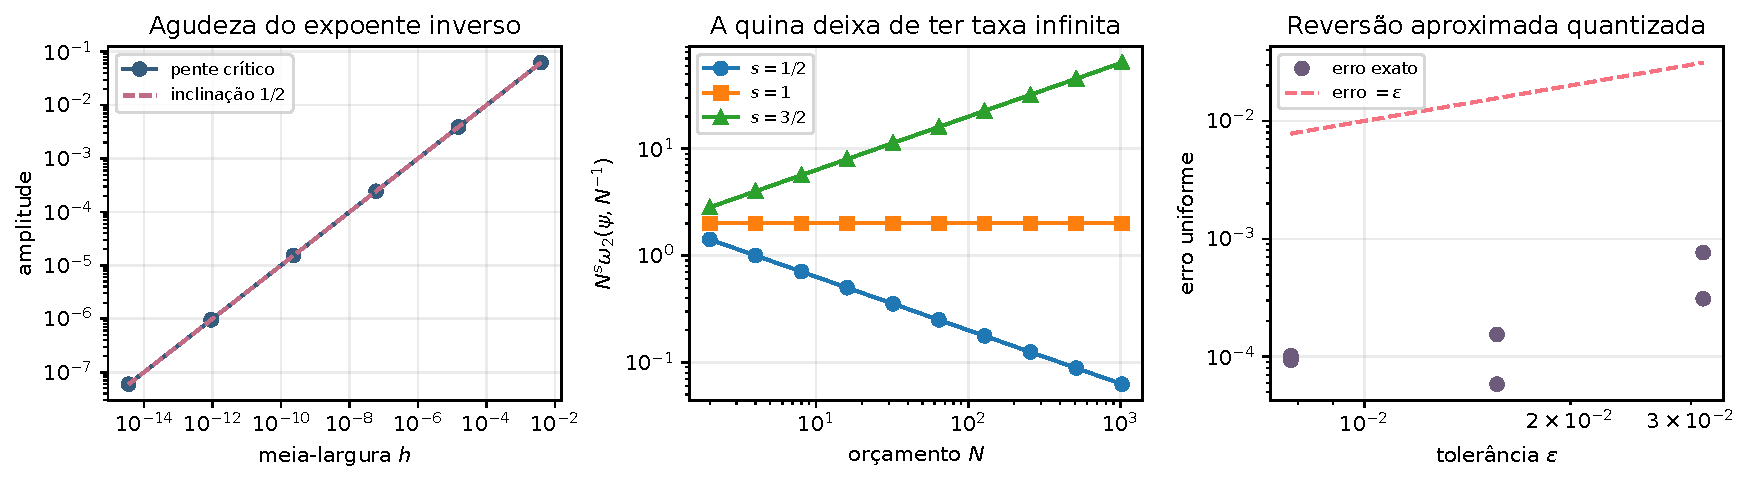
\includegraphics[width=.98\linewidth]{figuras/artigo_3/fig_reversibilidade_regularizada.pdf}
 \caption{Três diagnósticos da reversibilidade. À esquerda, o pente de tendas
 realiza o expoente crítico $\alpha/(\alpha+\gamma)$. Ao centro, o certificado
 atribui à quina exatamente a ordem um. À direita, a quantização de redes com
 quebras não diádicas permanece abaixo da tolerância prescrita.}
 \label{artigo_3:fig:regularized-reversibility}
\end{figure}

Os três mecanismos aparecem lado a lado na
\cref{artigo_3:fig:regularized-reversibility}; o painel do pente usa a
construção na biblioteca original do \cref{artigo_3:thm:critical-tent-comb}.

\subsection{Validação executável}

O programa \texttt{reversibilidade\_regularizada.py} executa uma auditoria
independente em aritmética \texttt{Fraction}. Ele:
\begin{enumerate}[label=(\roman*),leftmargin=2.2em]
 \item executa $2952$ idas e voltas exatas entre formas hinge e árvores
 canônicas, das quais $1160$ contêm ao menos uma região plana;
 \item verifica em todos os casos as duas cotas de folhas de
 \eqref{artigo_3:eq:canonical-tree-leaf-bounds};
 \item quantiza $84$ redes com quebras não diádicas e confere exatamente erro,
 número de folhas, inclinações não nulas e altura;
 \item testa $1260$ instâncias da desigualdade universal que sustenta
 \eqref{artigo_3:eq:universal-regularized-lower};
 \item reproduz a quina em dez escalas, a tenda profunda até $1024$ regiões e
 seis níveis do pente crítico, verificando em cada nível a perturbação, o erro,
 a altura, o número de folhas e a ausência de inclinações nulas na biblioteca
 original.
\end{enumerate}

A reversibilidade assume três formas. A biblioteca $\Library$ corresponde
exatamente à imagem rasa caracterizada por dados racionais, nós diádicos e
inclinações não nulas. A extensão marcada inclui regiões planas e produz uma
bijeção funcional rasa. Redes reais genéricas admitem aproximações inversas
com recursos explícitos. No nível de classes funcionais, o erro bruto possui a recíproca com perda do
\cref{artigo_3:thm:raw-lossy-inverse}, enquanto o certificado
\eqref{artigo_3:eq:self-roughness-certificate} fornece a caracterização direta e
inversa completa do \cref{artigo_3:thm:complete-besov-reversibility}. Essas três formas
separam representação exata, quantização e regularidade funcional.
\section{Conclusão}
As agendas de altura acompanham simultaneamente a geometria da malha e a quantização racional. A construção direta usa o expoente $\max\{1,s\}$ e, na faixa crítica com $q<\infty$, um fator logarítmico suficiente para a somabilidade. O piso aritmético uniforme exige crescimento de ordem $N^s$ quando a classe contém um intervalo de funções constantes.

O erro bruto e o crescimento das inclinações fornecem a regularidade inversa $\alpha/(\alpha+\gamma)$, aguda na biblioteca original para $0<\alpha\le\gamma$. A representação exata por redes rasas depende da racionalidade dos parâmetros e da posição diádica das quebras; redes com parâmetros reais admitem uma conversão aproximada com recursos explícitos.

O funcional de realização conserva a informação de segunda ordem que o melhor erro isolado perde. Sua cota inversa universal e o lado direto racional caracterizam os estratos de Besov sob as agendas declaradas. A mesma caracterização permanece válida para famílias de redes que contêm os aproximantes da biblioteca com sobrecusto linear de orçamento.




% V | fonte original: artigos/complemento_original_77/complemento.tex
\volumeparte{Complementos do manuscrito original}
% Reconstruído de artigos/complemento_original_77/complemento.tex


Este complemento conserva os três resultados da seção 6 e o lema 21.1 do documento original de 77 páginas. A numeração original é mantida para permitir o cruzamento com os três artigos da série. As hipóteses e conclusões foram reproduzidas integralmente; as remissões externas foram convertidas em referências textuais aos artigos correspondentes.

Usamos a biblioteca e a densidade das montagens racionais do primeiro artigo. Para o interpolante afim nos extremos de um intervalo $J$, vale a estimativa clássica
\begin{equation}
\|f-P_Jf\|_{\infty,J}\le\frac{|J|^2}{8}\|f''\|_{\infty,J}.
\label{complemento_original:eq:interpolation-remainder}
\end{equation}
O primeiro artigo contém a racionalização por valores nodais compartilhados. Os resultados abaixo servem de ponte entre as taxas uniformes, a comparação com nós livres e a teoria direta com altura do terceiro artigo.
\setcounter{section}{5}
% INICIO artigos/complemento_original_77/06_arvores_besov.tex
\section{Árvores diádicas, nós livres e regularidade de Besov}
\label{complemento_original:sec:dyadic-trees}

\subsection{Partições em árvore}

Se $K$ é uma célula diádica, uma partição em árvore $\Lambda$ é o conjunto de folhas de uma subárvore diádica finita com raiz $K$. Seja $P_\Lambda f$ o interpolante de $f$ nos extremos das folhas e defina
\begin{equation}
 \sigma_N^{\mathrm{dia}}(f)_\infty
 =\inf\{\|f-P_\Lambda f\|_{\infty,K}:\Lambda\text{ árvore},\ |\Lambda|\le N\}.
 \label{complemento_original:eq:sigma-dyadic}
\end{equation}

% MAPA complemento_original:6.1 | fonte artigos/complemento_original_77/06_arvores_besov.tex:13
\begin{theorem}[taxa garantida em árvores]\label{map:complemento_original:6.1}\label{complemento_original:thm:tree-rate}
Se $f\in C^2(K)$, $L=|K|$, $M=\|f''\|_{\infty,K}$ e $N\ge2$, então
\begin{equation}
 \sigma_N^{\mathrm{dia}}(f)_\infty\le\frac{ML^2}{2N^2}.
 \label{complemento_original:eq:tree-general}
\end{equation}
Se $N=2^r$, a constante melhora para
\begin{equation}
 \sigma_N^{\mathrm{dia}}(f)_\infty\le\frac{ML^2}{8N^2}.
 \label{complemento_original:eq:tree-power}
\end{equation}
Para qualquer árvore finita $\Lambda$ e $\delta>0$, há uma montagem racional na mesma árvore cujo erro é menor que $\|f-P_\Lambda f\|_\infty+\delta$.
\end{theorem}

\begin{proof}
Tome $r=\lfloor\log_2N\rfloor$ e refine $K$ uniformemente $r$ vezes. Há $2^r\le N$ folhas de largura $L2^{-r}$. Aplicando \eqref{complemento_original:eq:interpolation-remainder} em cada folha,
\[
 \|f-P_\Lambda f\|_\infty\le\frac{ML^2}{8}4^{-r}.
\]
Se $N=2^r$, resulta \eqref{complemento_original:eq:tree-power}. Em geral, $2^r>N/2$, logo $4^{-r}<4N^{-2}$, o que dá \eqref{complemento_original:eq:tree-general}. Para a racionalização, ordene os nós, aproxime os valores de $f$ por racionais compartilhados com erro menor que $\delta$ e evite igualdade entre vizinhos. Em cada folha, a diferença entre o interpolante exato e o racional é combinação convexa dos erros nodais; o argumento de densidade do primeiro artigo da série identifica cada peça como átomo.
\end{proof}

\subsection{Referência assintótica com nós livres}

Se $E_N^{\mathrm{lv}}(f)$ é o menor erro de interpolação linear com $N$
subintervalos e nós arbitrários, o regime de nós livres fornece a referência
contínua para comparação com árvores diádicas
\citep{artigo_1-deboor1973,artigo_1-burchard1974,artigo_1-deboor2001,artigo_1-powell1981,artigo_1-schumaker2007}.

% MAPA complemento_original:6.2 | fonte artigos/complemento_original_77/06_arvores_besov.tex:42
\begin{theorem}[cota assintótica com nós livres]\label{map:complemento_original:6.2}\label{complemento_original:thm:free-knots}
Para $f\in C^2[\alpha,\beta]$,
\begin{equation}
 \limsup_{N\to\infty}N^2E_N^{\mathrm{lv}}(f)
 \le\frac18\left(\int_\alpha^\beta |f''(x)|^{1/2}\dd x\right)^2.
 \label{complemento_original:eq:free-knot}
\end{equation}
\end{theorem}

\begin{proof}
Fixe $\eta>0$ e ponha $\rho_\eta=(|f''|+\eta)^{1/2}$ e $I_\eta=\int_\alpha^\beta\rho_\eta$. Como $\rho_\eta$ é contínua e estritamente positiva, existem nós $\alpha=x_{N,0}<\cdots<x_{N,N}=\beta$ tais que
\[
 \int_{x_{N,j-1}}^{x_{N,j}}\rho_\eta=I_\eta/N.
\]
O comprimento máximo das células tende uniformemente a zero. Em $J_j=[x_{N,j-1},x_{N,j}]$, \eqref{complemento_original:eq:interpolation-remainder} e $|f''|\le\rho_\eta^2$ dão
\[
 \|f-P_{J_j}f\|_{\infty,J_j}
 \le\frac18\left(\frac{I_\eta}{N}\right)^2
 \left(\frac{\sup_{J_j}\rho_\eta}{\inf_{J_j}\rho_\eta}\right)^2.
\]
Por continuidade uniforme e positividade, a última razão converge uniformemente a $1$. Assim,
\[
 \limsup_{N\to\infty}N^2E_N^{\mathrm{lv}}(f)\le I_\eta^2/8.
\]
Fazendo $\eta\downarrow0$ e usando convergência dominada, obtém-se \eqref{complemento_original:eq:free-knot}.
\end{proof}

A constante em \eqref{complemento_original:eq:free-knot} pertence ao regime de nós livres. A
constante sob restrição diádica será determinada nas seções de interpolação diádica do segundo artigo da série; é essa comparação, retomada explicitamente nos resultados de envelope e curvatura constante do segundo artigo, que mede o
custo da restrição de malha.

\subsection{Estimativa direta na escala de Besov}

As relações diretas e inversas entre aproximação por partes, splines e classes
de suavidade têm uma tradição ampla
\citep{artigo_2-birman1967,artigo_2-petrushev1988,artigo_2-devorepopov1988}. A formulação abaixo fixa a
escala estritamente diádica e o interpolante linear usados neste artigo.

Para $f\in C(K)$, defina
\begin{equation}
 \omega_2(f,t)_{\infty,K}
 =\sup_{\substack{0<h\le t\\x,x+2h\in K}}
 |f(x+2h)-2f(x+h)+f(x)|,
\end{equation}
e, para $0<s<2$,
\begin{equation}
 |f|_{B^s_{\infty,\infty}(K)}
 =\sup_{0<t\le|K|}t^{-s}\omega_2(f,t)_{\infty,K}.
 \label{complemento_original:eq:besov-seminorm}
\end{equation}

% MAPA complemento_original:6.3 | fonte artigos/complemento_original_77/06_arvores_besov.tex:93
\begin{theorem}[estimativa direta]\label{map:complemento_original:6.3}\label{complemento_original:thm:besov}
Se $0<s<2$, $|K|=L$ e o seminorma em \eqref{complemento_original:eq:besov-seminorm} é finito, então, para $N\ge2$,
\begin{equation}
 \sigma_N^{\mathrm{dia}}(f)_\infty
 \le C_sL^s|f|_{B^s_{\infty,\infty}(K)}N^{-s},
 \label{complemento_original:eq:besov-rate}
\end{equation}
onde $C_s$ independe de $f$ e $N$. Para todo $\delta>0$, uma montagem racional com no máximo $N$ folhas alcança o lado direito de \eqref{complemento_original:eq:besov-rate} acrescido de $\delta$.
\end{theorem}

\begin{proof}
A desigualdade de Whitney de ordem dois afirma que existe constante universal $C_W$ tal que, em todo intervalo $J$ \citep{artigo_2-whitney1957,artigo_1-devore1998},
\[
 E_1(f;J)_\infty:=\inf_{\ell\ \mathrm{afim}}\|f-\ell\|_{\infty,J}
 \le C_W\omega_2(f,|J|)_{\infty,J}.
\]
O interpolante de extremos $P_J$ reproduz funções afins e tem norma de operador no máximo $1$. Logo, para toda $\ell$ afim,
\[
 \|f-P_Jf\|_\infty
 \le\|f-\ell\|_\infty+\|P_J(f-\ell)\|_\infty
 \le2\|f-\ell\|_\infty.
\]
Tomando o ínfimo e observando que o módulo em $J\subset K$ não excede o de $K$,
\[
 \|f-P_Jf\|_{\infty,J}
 \le2C_W|J|^s|f|_{B^s_{\infty,\infty}(K)}.
\]
Refine $K$ uniformemente $r=\lfloor\log_2N\rfloor$ vezes. As folhas têm largura $L2^{-r}<2L/N$, e o máximo das estimativas locais prova \eqref{complemento_original:eq:besov-rate} com $C_s=2^{s+1}C_W$. A racionalização segue do último enunciado do \cref{complemento_original:thm:tree-rate}.
\end{proof}

% FIM artigos/complemento_original_77/06_arvores_besov.tex
\setcounter{section}{20}
% INICIO artigos/complemento_original_77/21_runge.tex
\section{Referência analítica para o exemplo de Runge}
Para
\begin{equation}
 f(x)=\frac{1}{1+25x^2},\qquad
 f''(x)=\frac{50(75x^2-1)}{(1+25x^2)^3},
 \label{complemento_original:eq:runge}
\end{equation}
o refinamento certificado do primeiro artigo usa majorantes intervalares racionais. O máximo analítico abaixo é uma referência independente para medir a folga do certificado, sem substituir a garantia intervalar.

% MAPA complemento_original:21.1 | fonte artigos/complemento_original_77/21_runge.tex:10
\begin{lemma}[majorante local da função de Runge]\label{map:complemento_original:21.1}\label{complemento_original:lem:runge-majorant}
Em todo intervalo fechado $J\subset[-1,1]$, o máximo de $|f''|$ é atingido em um extremo de $J$ ou em um ponto de $\{0,-0{,}2,0{,}2\}\cap J$.
\end{lemma}

\begin{proof}
Derivando \eqref{complemento_original:eq:runge},
\[
 f'''(x)=\frac{7500x(2-50x^2)}{(1+25x^2)^4},
\]
cujos únicos zeros são $0$ e $\pm0{,}2$. Um máximo interior não nulo de $|f''|$ deve ser ponto crítico de $f''$; os zeros de $f''$ têm módulo zero e não introduzem máximos positivos. Restam os três pontos críticos e os extremos do intervalo.
\end{proof}
% FIM artigos/complemento_original_77/21_runge.tex


\clearpage\part*{Correspondência documental e formal}\addcontentsline{toc}{part}{Correspondência documental e formal}
\section*{Estado da correspondência}
As categorias abaixo reproduzem a matriz recebida. Correspondência inspecionada identifica declarações relevantes; integração à base exige as pontes documentadas. Contratos abstratos, cobertura parcial e pendências conservam seu alcance. O arquivo \texttt{mapas/MAPA\_TEX\_LEAN.md} reúne os nomes Lean, os caminhos e as posições de cada resultado.

Todos os 42 casos do dossiê de pendências estão fechados: 41 por prova Lean compilada e auditada e III.12.3 por prova textual sincronizada. Permanecem como ressalvas: a reverificação da leitura de $g(t_0)$ em I.4.3 contra o enunciado Lean; o enunciado de IV.5.4, cuja cota impressa era falsa para $M=0$ (contraexemplo documentado e certificado separadamente) e foi corrigida no texto; os modelos de custo de III.9.1 (operações unitárias; o desempate por $\kappa$ não está no programa denso) e de III.9.3 (o custo da aritmética racional em bits é hipótese do modelo). Os demais estados e ressalvas constam das linhas abaixo. As correspondências herdadas não são promovidas a provas verificadas por esta revisão.

Até 13/11/2026, 41 resultados antes pendentes passaram ao estado ``Formalizado e compilado'': provas Lean compiladas com Lean/Mathlib 4.28.0 nas bibliotecas \texttt{Pendencias} e \texttt{PendenciasParte1} dos ambientes \texttt{artigo\_2} e \texttt{base\_integrada}, sem \texttt{sorry} e apenas com os axiomas \texttt{propext}, \texttt{Classical.choice} e \texttt{Quot.sound}. Os demais estados e ressalvas seguem descritos acima.

\subsection*{Parte I}
\small
\begin{longtable}{@{}p{.11\linewidth}p{.09\linewidth}p{.09\linewidth}p{.59\linewidth}@{}}
\toprule Resultado & Original & Página & Estado e ressalva\\\midrule\endhead
\hyperref[map:artigo_1:2.1]{I.2.1} & 2.1 & \pageref{map:artigo_1:2.1} & Correspondência inspecionada\\[4pt]
\hyperref[map:artigo_1:2.2]{I.2.2} & 2.2 & \pageref{map:artigo_1:2.2} & Correspondência inspecionada\\[4pt]
\hyperref[map:artigo_1:2.3]{I.2.3} & 2.3 & \pageref{map:artigo_1:2.3} & Correspondência inspecionada\\[4pt]
\hyperref[map:artigo_1:2.4]{I.2.4} & 2.4 & \pageref{map:artigo_1:2.4} & Correspondência inspecionada\\[4pt]
\hyperref[map:artigo_1:2.5]{I.2.5} & 2.5 & \pageref{map:artigo_1:2.5} & Correspondência inspecionada\\[4pt]
\hyperref[map:artigo_1:3.1]{I.3.1} & 3.1 & \pageref{map:artigo_1:3.1} & Correspondência inspecionada\\[4pt]
\hyperref[map:artigo_1:3.2]{I.3.2} & 3.2 & \pageref{map:artigo_1:3.2} & Correspondência inspecionada\\[4pt]
\hyperref[map:artigo_1:3.3]{I.3.3} & 3.3 & \pageref{map:artigo_1:3.3} & Correspondência inspecionada\\[4pt]
\hyperref[map:artigo_1:3.4]{I.3.4} & 3.4 & \pageref{map:artigo_1:3.4} & Correspondência inspecionada\\[4pt]
\hyperref[map:artigo_1:3.5]{I.3.5} & 3.5 & \pageref{map:artigo_1:3.5} & Correspondência inspecionada\\[4pt]
\hyperref[map:artigo_1:3.6]{I.3.6} & 3.6 & \pageref{map:artigo_1:3.6} & Correspondência inspecionada\\[4pt]
\hyperref[map:artigo_1:4.1]{I.4.1} & 4.1 & \pageref{map:artigo_1:4.1} & Integrado à base. Identificação com os tipos concretos da v2 provada nos módulos NormalizationAtoms, Contracts, Enumerations, Classes, Errors e ReLU. Hipóteses, domínio, função e orçamentos preservados.\\[4pt]
\hyperref[map:artigo_1:4.2]{I.4.2} & 4.2 & \pageref{map:artigo_1:4.2} & Correspondência inspecionada\\[4pt]
\hyperref[map:artigo_1:4.3]{I.4.3} & 4.3 & \pageref{map:artigo_1:4.3} & Divergência documentada. O operador de extensão normalizado foi integrado à classe concreta da Fase 2. O enunciado TeX deste volume lê $g(t_0)$ como o valor em $t_0$ da primeira peça ($t_0$ pode estar fora de $K$); essa leitura não foi reverificada contra o enunciado Lean.\\[4pt]
\hyperref[map:artigo_1:4.4]{I.4.4} & 4.4 & \pageref{map:artigo_1:4.4} & Correspondência inspecionada\\[4pt]
\hyperref[map:artigo_1:4.5]{I.4.5} & 4.5 & \pageref{map:artigo_1:4.5} & Correspondência inspecionada\\[4pt]
\hyperref[map:artigo_1:5.1]{I.5.1} & 5.1 & \pageref{map:artigo_1:5.1} & Correspondência inspecionada\\[4pt]
\hyperref[map:artigo_1:5.2]{I.5.2} & 5.2 & \pageref{map:artigo_1:5.2} & Correspondência inspecionada\\[4pt]
\hyperref[map:artigo_1:6.1]{I.6.1} & 7.1 & \pageref{map:artigo_1:6.1} & Correspondência inspecionada\\[4pt]
\hyperref[map:artigo_1:6.2]{I.6.2} & 7.2 & \pageref{map:artigo_1:6.2} & Correspondência inspecionada\\[4pt]
\hyperref[map:artigo_1:6.3]{I.6.3} & 7.3 & \pageref{map:artigo_1:6.3} & Formalizado e compilado. Provas: \code{PendenciasParte1.certRefine, PendenciasParte1.certified_refinement} (raízes contidas em $[\alpha,\beta]$) e, para coberturas diádicas externas, \code{CoberturaExterna.certRefineProjected, CoberturaExterna.projected_certificate_sound}. Ver declarações e contratos nas fontes Lean. Compilado com Lean/Mathlib 4.28.0 (\texttt{lake build PendenciasParte1}); axiomas: \texttt{propext}, \texttt{Classical.choice}, \texttt{Quot.sound}. Ressalva: o refinamento é uma definição \texttt{noncomputable}, e as escolhas nodais e os endereços são dados por existência, como no texto.\\[4pt]
\hyperref[map:artigo_1:6.4]{I.6.4} & 7.4 & \pageref{map:artigo_1:6.4} & Formalizado e compilado. Provas: \code{PendenciasParte1.certified_refinement} (raízes contidas em $[\alpha,\beta]$) e, para coberturas diádicas externas, \code{CoberturaExterna.refinement_contract_external, CoberturaExterna.certified_refinement_external}, com o exemplo $[1/3,2/3]$ em \code{CoberturaExterna.thirds_success}. Ver declarações e contratos nas fontes Lean. Compilado com Lean/Mathlib 4.28.0 (\texttt{lake build PendenciasParte1}); axiomas: \texttt{propext}, \texttt{Classical.choice}, \texttt{Quot.sound}. Ressalva: término e correção sob o contrato de majorante (hipótese de entrada), sem certificar uma implementação executável ligada ao avaliador intervalar.\\[4pt]
\hyperref[map:artigo_1:6.5]{I.6.5} & 7.5 & \pageref{map:artigo_1:6.5} & Correspondência inspecionada\\[4pt]
\hyperref[map:artigo_1:6.6]{I.6.6} & 7.6 & \pageref{map:artigo_1:6.6} & Correspondência inspecionada\\[4pt]
\bottomrule\end{longtable}\normalsize

\subsection*{Parte II}
\small
\begin{longtable}{@{}p{.11\linewidth}p{.09\linewidth}p{.09\linewidth}p{.59\linewidth}@{}}
\toprule Resultado & Original & Página & Estado e ressalva\\\midrule\endhead
\hyperref[map:normalizacao:2.1]{II.2.1} & -- & \pageref{map:normalizacao:2.1} & Correspondência inspecionada. Resultado recebido preservado. A identificação dos tipos de átomos, endereços, classes e erros com a v2 está provada nas pontes Normalization; consultar INTEGRACAO\_NORMALIZACAO.md.\\[4pt]
\hyperref[map:normalizacao:2.2]{II.2.2} & -- & \pageref{map:normalizacao:2.2} & Correspondência inspecionada. Resultado recebido preservado. A identificação dos tipos de átomos, endereços, classes e erros com a v2 está provada nas pontes Normalization; consultar INTEGRACAO\_NORMALIZACAO.md.\\[4pt]
\hyperref[map:normalizacao:2.3]{II.2.3} & -- & \pageref{map:normalizacao:2.3} & Correspondência inspecionada. Resultado recebido preservado. A identificação dos tipos de átomos, endereços, classes e erros com a v2 está provada nas pontes Normalization; consultar INTEGRACAO\_NORMALIZACAO.md.\\[4pt]
\hyperref[map:normalizacao:2.4]{II.2.4} & -- & \pageref{map:normalizacao:2.4} & Integrado à base. Identificação com os tipos concretos da v2 provada nos módulos NormalizationAtoms, Contracts, Enumerations, Classes, Errors e ReLU. Hipóteses, domínio, função e orçamentos preservados.\\[4pt]
\hyperref[map:normalizacao:2.5]{II.2.5} & -- & \pageref{map:normalizacao:2.5} & Integrado à base. Identificação com os tipos concretos da v2 provada nos módulos NormalizationAtoms, Contracts, Enumerations, Classes, Errors e ReLU. Hipóteses, domínio, função e orçamentos preservados.\\[4pt]
\hyperref[map:normalizacao:3.1]{II.3.1} & -- & \pageref{map:normalizacao:3.1} & Integrado à base. Identificação com os tipos concretos da v2 provada nos módulos NormalizationAtoms, Contracts, Enumerations, Classes, Errors e ReLU. Hipóteses, domínio, função e orçamentos preservados.\\[4pt]
\hyperref[map:normalizacao:3.2]{II.3.2} & -- & \pageref{map:normalizacao:3.2} & Correspondência inspecionada. Resultado recebido preservado. A identificação dos tipos de átomos, endereços, classes e erros com a v2 está provada nas pontes Normalization; consultar INTEGRACAO\_NORMALIZACAO.md.\\[4pt]
\hyperref[map:normalizacao:3.3]{II.3.3} & -- & \pageref{map:normalizacao:3.3} & Correspondência inspecionada. Resultado recebido preservado. A identificação dos tipos de átomos, endereços, classes e erros com a v2 está provada nas pontes Normalization; consultar INTEGRACAO\_NORMALIZACAO.md.\\[4pt]
\hyperref[map:normalizacao:3.4]{II.3.4} & -- & \pageref{map:normalizacao:3.4} & Correspondência inspecionada. Resultado recebido preservado. A identificação dos tipos de átomos, endereços, classes e erros com a v2 está provada nas pontes Normalization; consultar INTEGRACAO\_NORMALIZACAO.md.\\[4pt]
\hyperref[map:normalizacao:3.5]{II.3.5} & -- & \pageref{map:normalizacao:3.5} & Integrado à base. Identificação com os tipos concretos da v2 provada nos módulos NormalizationAtoms, Contracts, Enumerations, Classes, Errors e ReLU. Hipóteses, domínio, função e orçamentos preservados.\\[4pt]
\hyperref[map:normalizacao:3.6]{II.3.6} & -- & \pageref{map:normalizacao:3.6} & Integrado à base. Identificação com os tipos concretos da v2 provada nos módulos NormalizationAtoms, Contracts, Enumerations, Classes, Errors e ReLU. Hipóteses, domínio, função e orçamentos preservados.\\[4pt]
\hyperref[map:normalizacao:4.1]{II.4.1} & -- & \pageref{map:normalizacao:4.1} & Correspondência inspecionada. Resultado recebido preservado. A identificação dos tipos de átomos, endereços, classes e erros com a v2 está provada nas pontes Normalization; consultar INTEGRACAO\_NORMALIZACAO.md.\\[4pt]
\hyperref[map:normalizacao:4.2]{II.4.2} & -- & \pageref{map:normalizacao:4.2} & Integrado à base. Identificação com os tipos concretos da v2 provada nos módulos NormalizationAtoms, Contracts, Enumerations, Classes, Errors e ReLU. Hipóteses, domínio, função e orçamentos preservados.\\[4pt]
\hyperref[map:normalizacao:4.3]{II.4.3} & -- & \pageref{map:normalizacao:4.3} & Integrado à base. Identificação com os tipos concretos da v2 provada nos módulos NormalizationAtoms, Contracts, Enumerations, Classes, Errors e ReLU. Hipóteses, domínio, função e orçamentos preservados.\\[4pt]
\hyperref[map:normalizacao:4.4]{II.4.4} & -- & \pageref{map:normalizacao:4.4} & Correspondência inspecionada. Resultado recebido preservado. A identificação dos tipos de átomos, endereços, classes e erros com a v2 está provada nas pontes Normalization; consultar INTEGRACAO\_NORMALIZACAO.md.\\[4pt]
\hyperref[map:normalizacao:4.5]{II.4.5} & -- & \pageref{map:normalizacao:4.5} & Integrado à base. Identificação com os tipos concretos da v2 provada nos módulos NormalizationAtoms, Contracts, Enumerations, Classes, Errors e ReLU. Hipóteses, domínio, função e orçamentos preservados.\\[4pt]
\hyperref[map:normalizacao:4.6]{II.4.6} & -- & \pageref{map:normalizacao:4.6} & Correspondência inspecionada. Resultado recebido preservado. A identificação dos tipos de átomos, endereços, classes e erros com a v2 está provada nas pontes Normalization; consultar INTEGRACAO\_NORMALIZACAO.md.\\[4pt]
\hyperref[map:normalizacao:4.7]{II.4.7} & -- & \pageref{map:normalizacao:4.7} & Integrado à base. Identificação com os tipos concretos da v2 provada nos módulos NormalizationAtoms, Contracts, Enumerations, Classes, Errors e ReLU. Hipóteses, domínio, função e orçamentos preservados.\\[4pt]
\hyperref[map:normalizacao:5.1]{II.5.1} & -- & \pageref{map:normalizacao:5.1} & Correspondência inspecionada. Resultado recebido preservado. A identificação dos tipos de átomos, endereços, classes e erros com a v2 está provada nas pontes Normalization; consultar INTEGRACAO\_NORMALIZACAO.md.\\[4pt]
\hyperref[map:normalizacao:5.2]{II.5.2} & -- & \pageref{map:normalizacao:5.2} & Integrado à base. Identificação com os tipos concretos da v2 provada nos módulos NormalizationAtoms, Contracts, Enumerations, Classes, Errors e ReLU. Hipóteses, domínio, função e orçamentos preservados.\\[4pt]
\hyperref[map:normalizacao:5.3]{II.5.3} & -- & \pageref{map:normalizacao:5.3} & Integrado à base. Identificação com os tipos concretos da v2 provada nos módulos NormalizationAtoms, Contracts, Enumerations, Classes, Errors e ReLU. Hipóteses, domínio, função e orçamentos preservados.\\[4pt]
\hyperref[map:normalizacao:5.4]{II.5.4} & -- & \pageref{map:normalizacao:5.4} & Correspondência inspecionada. Resultado recebido preservado. A identificação dos tipos de átomos, endereços, classes e erros com a v2 está provada nas pontes Normalization; consultar INTEGRACAO\_NORMALIZACAO.md.\\[4pt]
\hyperref[map:normalizacao:5.5]{II.5.5} & -- & \pageref{map:normalizacao:5.5} & Correspondência inspecionada. Resultado recebido preservado. A identificação dos tipos de átomos, endereços, classes e erros com a v2 está provada nas pontes Normalization; consultar INTEGRACAO\_NORMALIZACAO.md.\\[4pt]
\hyperref[map:normalizacao:5.6]{II.5.6} & -- & \pageref{map:normalizacao:5.6} & Integrado à base. Identificação com os tipos concretos da v2 provada nos módulos NormalizationAtoms, Contracts, Enumerations, Classes, Errors e ReLU. Hipóteses, domínio, função e orçamentos preservados.\\[4pt]
\hyperref[map:normalizacao:6.1]{II.6.1} & -- & \pageref{map:normalizacao:6.1} & Integrado à base. Identificação com os tipos concretos da v2 provada nos módulos NormalizationAtoms, Contracts, Enumerations, Classes, Errors e ReLU. Hipóteses, domínio, função e orçamentos preservados.\\[4pt]
\hyperref[map:normalizacao:6.2]{II.6.2} & -- & \pageref{map:normalizacao:6.2} & Integrado à base. Identificação com os tipos concretos da v2 provada nos módulos NormalizationAtoms, Contracts, Enumerations, Classes, Errors e ReLU. Hipóteses, domínio, função e orçamentos preservados.\\[4pt]
\hyperref[map:normalizacao:6.3]{II.6.3} & -- & \pageref{map:normalizacao:6.3} & Integrado à base. Identificação com os tipos concretos da v2 provada nos módulos NormalizationAtoms, Contracts, Enumerations, Classes, Errors e ReLU. Hipóteses, domínio, função e orçamentos preservados.\\[4pt]
\hyperref[map:normalizacao:6.4]{II.6.4} & -- & \pageref{map:normalizacao:6.4} & Integrado à base. Identificação com os tipos concretos da v2 provada nos módulos NormalizationAtoms, Contracts, Enumerations, Classes, Errors e ReLU. Hipóteses, domínio, função e orçamentos preservados.\\[4pt]
\hyperref[map:normalizacao:6.5]{II.6.5} & -- & \pageref{map:normalizacao:6.5} & Correspondência inspecionada. Resultado recebido preservado. A identificação dos tipos de átomos, endereços, classes e erros com a v2 está provada nas pontes Normalization; consultar INTEGRACAO\_NORMALIZACAO.md.\\[4pt]
\hyperref[map:normalizacao:7.1]{II.7.1} & -- & \pageref{map:normalizacao:7.1} & Correspondência inspecionada. Resultado recebido preservado. A identificação dos tipos de átomos, endereços, classes e erros com a v2 está provada nas pontes Normalization; consultar INTEGRACAO\_NORMALIZACAO.md.\\[4pt]
\hyperref[map:normalizacao:7.2]{II.7.2} & -- & \pageref{map:normalizacao:7.2} & Correspondência inspecionada. Resultado recebido preservado. A identificação dos tipos de átomos, endereços, classes e erros com a v2 está provada nas pontes Normalization; consultar INTEGRACAO\_NORMALIZACAO.md.\\[4pt]
\hyperref[map:normalizacao:7.3]{II.7.3} & -- & \pageref{map:normalizacao:7.3} & Correspondência inspecionada. Resultado recebido preservado. A identificação dos tipos de átomos, endereços, classes e erros com a v2 está provada nas pontes Normalization; consultar INTEGRACAO\_NORMALIZACAO.md.\\[4pt]
\hyperref[map:normalizacao:7.4]{II.7.4} & -- & \pageref{map:normalizacao:7.4} & Correspondência inspecionada. Resultado recebido preservado. A identificação dos tipos de átomos, endereços, classes e erros com a v2 está provada nas pontes Normalization; consultar INTEGRACAO\_NORMALIZACAO.md.\\[4pt]
\hyperref[map:normalizacao:8.1]{II.8.1} & -- & \pageref{map:normalizacao:8.1} & Correspondência inspecionada. Resultado recebido preservado. A identificação dos tipos de átomos, endereços, classes e erros com a v2 está provada nas pontes Normalization; consultar INTEGRACAO\_NORMALIZACAO.md.\\[4pt]
\hyperref[map:normalizacao:8.2]{II.8.2} & -- & \pageref{map:normalizacao:8.2} & Correspondência inspecionada. Resultado recebido preservado. A identificação dos tipos de átomos, endereços, classes e erros com a v2 está provada nas pontes Normalization; consultar INTEGRACAO\_NORMALIZACAO.md.\\[4pt]
\hyperref[map:normalizacao:8.3]{II.8.3} & -- & \pageref{map:normalizacao:8.3} & Correspondência inspecionada. Resultado recebido preservado. A identificação dos tipos de átomos, endereços, classes e erros com a v2 está provada nas pontes Normalization; consultar INTEGRACAO\_NORMALIZACAO.md.\\[4pt]
\hyperref[map:normalizacao:8.4]{II.8.4} & -- & \pageref{map:normalizacao:8.4} & Integrado à base. Identificação com os tipos concretos da v2 provada nos módulos NormalizationAtoms, Contracts, Enumerations, Classes, Errors e ReLU. Hipóteses, domínio, função e orçamentos preservados.\\[4pt]
\hyperref[map:normalizacao:8.5]{II.8.5} & -- & \pageref{map:normalizacao:8.5} & Correspondência inspecionada. Resultado recebido preservado. A identificação dos tipos de átomos, endereços, classes e erros com a v2 está provada nas pontes Normalization; consultar INTEGRACAO\_NORMALIZACAO.md.\\[4pt]
\hyperref[map:normalizacao:8.6]{II.8.6} & -- & \pageref{map:normalizacao:8.6} & Integrado à base. Identificação com os tipos concretos da v2 provada nos módulos NormalizationAtoms, Contracts, Enumerations, Classes, Errors e ReLU. Hipóteses, domínio, função e orçamentos preservados.\\[4pt]
\hyperref[map:normalizacao:8.7]{II.8.7} & -- & \pageref{map:normalizacao:8.7} & Integrado à base. Identificação com os tipos concretos da v2 provada nos módulos NormalizationAtoms, Contracts, Enumerations, Classes, Errors e ReLU. Hipóteses, domínio, função e orçamentos preservados.\\[4pt]
\bottomrule\end{longtable}\normalsize

\subsection*{Parte III}
\small
\begin{longtable}{@{}p{.11\linewidth}p{.09\linewidth}p{.09\linewidth}p{.59\linewidth}@{}}
\toprule Resultado & Original & Página & Estado e ressalva\\\midrule\endhead
\hyperref[map:artigo_2:2.1]{III.2.1} & -- & \pageref{map:artigo_2:2.1} & Correspondência inspecionada\\[4pt]
\hyperref[map:artigo_2:2.2]{III.2.2} & -- & \pageref{map:artigo_2:2.2} & Correspondência inspecionada\\[4pt]
\hyperref[map:artigo_2:2.3]{III.2.3} & -- & \pageref{map:artigo_2:2.3} & Formalizado e compilado. Cota de interpolação provada com \texttt{ContDiffOn} de ordem 2 em \texttt{Icc a b} e \texttt{derivWithin}, via extensão $C^2$ portada da Fase 3 (\texttt{Pendencias/Extensao.lean}); densidade e forma ReLU já batiam. Compilado com Lean/Mathlib 4.28.0 (\texttt{lake build Pendencias}); axiomas: \texttt{propext}, \texttt{Classical.choice}, \texttt{Quot.sound}. Ressalva anterior: Resultados globais ou classe FRM usam regularidade $C^2$ na reta. O artigo admite $C^2$ no intervalo; transportar a extensão Fase3.extF e preservar valores, erros e curvatura. Conferir individualmente as hipóteses dos componentes citados.\\[4pt]
\hyperref[map:artigo_2:3.1]{III.3.1} & 8.1 & \pageref{map:artigo_2:3.1} & Correspondência inspecionada\\[4pt]
\hyperref[map:artigo_2:3.2]{III.3.2} & 8.2 & \pageref{map:artigo_2:3.2} & Correspondência inspecionada\\[4pt]
\hyperref[map:artigo_2:3.3]{III.3.3} & 8.3 & \pageref{map:artigo_2:3.3} & Correspondência inspecionada\\[4pt]
\hyperref[map:artigo_2:3.4]{III.3.4} & 8.4 & \pageref{map:artigo_2:3.4} & Correspondência inspecionada\\[4pt]
\hyperref[map:artigo_2:3.5]{III.3.5} & 8.5 & \pageref{map:artigo_2:3.5} & Observação editorial. Observação ou diagnóstico do texto; não é um teorema Lean autônomo.\\[4pt]
\hyperref[map:artigo_2:3.6]{III.3.6} & 8.6 & \pageref{map:artigo_2:3.6} & Correspondência inspecionada\\[4pt]
\hyperref[map:artigo_2:3.7]{III.3.7} & 8.7 & \pageref{map:artigo_2:3.7} & Correspondência inspecionada\\[4pt]
\hyperref[map:artigo_2:3.8]{III.3.8} & 8.8 & \pageref{map:artigo_2:3.8} & Observação editorial. Observação ou diagnóstico do texto; não é um teorema Lean autônomo.\\[4pt]
\hyperref[map:artigo_2:3.9]{III.3.9} & 8.9 & \pageref{map:artigo_2:3.9} & Correspondência inspecionada\\[4pt]
\hyperref[map:artigo_2:3.10]{III.3.10} & 8.10 & \pageref{map:artigo_2:3.10} & Observação editorial. Observação ou diagnóstico do texto; não é um teorema Lean autônomo.\\[4pt]
\hyperref[map:artigo_2:3.11]{III.3.11} & 8.11 & \pageref{map:artigo_2:3.11} & Correspondência inspecionada\\[4pt]
\hyperref[map:artigo_2:3.12]{III.3.12} & 8.12 & \pageref{map:artigo_2:3.12} & Formalizado e compilado. Provas: \code{Pendencias.coding_formats_comparison}. Ver declarações e contratos nas fontes Lean. Compilado com Lean/Mathlib 4.28.0 (\texttt{lake build Pendencias}); axiomas: \texttt{propext}, \texttt{Classical.choice}, \texttt{Quot.sound}. Ressalva anterior, superada: \code{coding_gap_family} provava só a cadeia de átomos para $N$ par; a árvore de raiz única $J_{H-1-r,0}$, com $N=2^r$, é construída por \code{Pendencias.famTree} e tratada em \code{Pendencias.coding_formats_comparison}.\\[4pt]
\hyperref[map:artigo_2:3.13]{III.3.13} & 8.13 & \pageref{map:artigo_2:3.13} & Correspondência inspecionada\\[4pt]
\hyperref[map:artigo_2:3.14]{III.3.14} & 8.14 & \pageref{map:artigo_2:3.14} & Correspondência inspecionada\\[4pt]
\hyperref[map:artigo_2:3.15]{III.3.15} & 8.15 & \pageref{map:artigo_2:3.15} & Formalizado e compilado. Classe \texttt{FRMIcc R M} ($C^2$ apenas em $[0,1]$, $f''$ unilateral); $\mathrm{FRM}\subseteq\mathrm{FRMIcc}$ e \texttt{extF f 0 1} pertence a FRM e coincide com $f$ em $[0,1]$; $|f'|\le 4R+M/2$ com $f'$ unilateral. Compilado com Lean/Mathlib 4.28.0 (\texttt{lake build Pendencias}); axiomas: \texttt{propext}, \texttt{Classical.choice}, \texttt{Quot.sound}. Ressalva anterior: Resultados globais ou classe FRM usam regularidade $C^2$ na reta. O artigo admite $C^2$ no intervalo; transportar a extensão Fase3.extF e preservar valores, erros e curvatura. Conferir individualmente as hipóteses dos componentes citados.\\[4pt]
\hyperref[map:artigo_2:3.16]{III.3.16} & 8.16 & \pageref{map:artigo_2:3.16} & Formalizado e compilado. Classe \texttt{FRMIcc R M} como em III.3.15; mesma árvore determinística \texttt{uniformTree (jvals f r)}, que só amostra $f$ em $[0,1]$, e consequência para todo $N\ge 2$. Compilado com Lean/Mathlib 4.28.0 (\texttt{lake build Pendencias}); axiomas: \texttt{propext}, \texttt{Classical.choice}, \texttt{Quot.sound}. Ressalva anterior: Resultados globais ou classe FRM usam regularidade $C^2$ na reta. O artigo admite $C^2$ no intervalo; transportar a extensão Fase3.extF e preservar valores, erros e curvatura. Conferir individualmente as hipóteses dos componentes citados.\\[4pt]
\hyperref[map:artigo_2:3.17]{III.3.17} & 8.17 & \pageref{map:artigo_2:3.17} & Formalizado e compilado. Classe \texttt{FRMIcc R M} como em III.3.15; $n_\varepsilon$ e $H_\varepsilon$ inalterados; \texttt{jointErr}, \texttt{heightFor} e \texttt{supDist} só dependem de $f$ em $[0,1]$. Compilado com Lean/Mathlib 4.28.0 (\texttt{lake build Pendencias}); axiomas: \texttt{propext}, \texttt{Classical.choice}, \texttt{Quot.sound}. Ressalva anterior: Resultados globais ou classe FRM usam regularidade $C^2$ na reta. O artigo admite $C^2$ no intervalo; transportar a extensão Fase3.extF e preservar valores, erros e curvatura. Conferir individualmente as hipóteses dos componentes citados.\\[4pt]
\hyperref[map:artigo_2:3.18]{III.3.18} & 8.18 & \pageref{map:artigo_2:3.18} & Formalizado e compilado. Classe \texttt{FRMIcc R M} como em III.3.15; as coberturas de FRMIcc e FRM coincidem (\texttt{isCover\_iff}), logo as entropias coincidem; codebook transportado. Compilado com Lean/Mathlib 4.28.0 (\texttt{lake build Pendencias}); axiomas: \texttt{propext}, \texttt{Classical.choice}, \texttt{Quot.sound}. Ressalva anterior: Resultados globais ou classe FRM usam regularidade $C^2$ na reta. O artigo admite $C^2$ no intervalo; transportar a extensão Fase3.extF e preservar valores, erros e curvatura. Conferir individualmente as hipóteses dos componentes citados.\\[4pt]
\hyperref[map:artigo_2:3.19]{III.3.19} & 8.19 & \pageref{map:artigo_2:3.19} & Correspondência inspecionada\\[4pt]
\hyperref[map:artigo_2:3.20]{III.3.20} & 8.20 & \pageref{map:artigo_2:3.20} & Correspondência inspecionada\\[4pt]
\hyperref[map:artigo_2:3.21]{III.3.21} & 8.21 & \pageref{map:artigo_2:3.21} & Correspondência inspecionada\\[4pt]
\hyperref[map:artigo_2:3.22]{III.3.22} & 8.22 & \pageref{map:artigo_2:3.22} & Correspondência inspecionada\\[4pt]
\hyperref[map:artigo_2:3.23]{III.3.23} & 8.23 & \pageref{map:artigo_2:3.23} & Correspondência inspecionada\\[4pt]
\hyperref[map:artigo_2:3.24]{III.3.24} & 8.24 & \pageref{map:artigo_2:3.24} & Correspondência inspecionada\\[4pt]
\hyperref[map:artigo_2:3.25]{III.3.25} & 8.25 & \pageref{map:artigo_2:3.25} & Formalizado e compilado. Provas: \code{Pendencias.gen_eq_RepCat, Pendencias.enumSelect_eq_canon}. Ver declarações e contratos nas fontes Lean. Compilado com Lean/Mathlib 4.28.0 (\texttt{lake build Pendencias}); axiomas: \texttt{propext}, \texttt{Classical.choice}, \texttt{Quot.sound}. Ressalva anterior: A recorrência ou existência matemática tem prova; falta implementar e certificar a execução e a reconstrução com comparação exata.\\[4pt]
\hyperref[map:artigo_2:4.1]{III.4.1} & 9.1 & \pageref{map:artigo_2:4.1} & Correspondência inspecionada\\[4pt]
\hyperref[map:artigo_2:4.2]{III.4.2} & 9.2 & \pageref{map:artigo_2:4.2} & Correspondência inspecionada\\[4pt]
\hyperref[map:artigo_2:4.3]{III.4.3} & 9.3 & \pageref{map:artigo_2:4.3} & Correspondência inspecionada\\[4pt]
\hyperref[map:artigo_2:4.4]{III.4.4} & 9.4 & \pageref{map:artigo_2:4.4} & Correspondência inspecionada\\[4pt]
\hyperref[map:artigo_2:4.5]{III.4.5} & 9.5 & \pageref{map:artigo_2:4.5} & Correspondência inspecionada\\[4pt]
\hyperref[map:artigo_2:4.6]{III.4.6} & 9.6 & \pageref{map:artigo_2:4.6} & Observação editorial. Observação ou diagnóstico do texto; não é um teorema Lean autônomo.\\[4pt]
\hyperref[map:artigo_2:5.1]{III.5.1} & 10.1 & \pageref{map:artigo_2:5.1} & Correspondência inspecionada\\[4pt]
\hyperref[map:artigo_2:5.2]{III.5.2} & 10.2 & \pageref{map:artigo_2:5.2} & Correspondência inspecionada\\[4pt]
\hyperref[map:artigo_2:6.1]{III.6.1} & 11.1 & \pageref{map:artigo_2:6.1} & Correspondência inspecionada\\[4pt]
\hyperref[map:artigo_2:6.2]{III.6.2} & 11.2 & \pageref{map:artigo_2:6.2} & Correspondência inspecionada\\[4pt]
\hyperref[map:artigo_2:6.3]{III.6.3} & 11.3 & \pageref{map:artigo_2:6.3} & Formalizado e compilado. Provas: \code{Pendencias.DPprog.fixTable_cost, Pendencias.DPprog.fixRoot_spec}. Ver declarações e contratos nas fontes Lean. Compilado com Lean/Mathlib 4.28.0 (\texttt{lake build Pendencias}); axiomas: \texttt{propext}, \texttt{Classical.choice}, \texttt{Quot.sound}. Ressalva anterior: A recorrência ou existência matemática tem prova; falta implementar e certificar a execução e a reconstrução com comparação exata.\\[4pt]
\hyperref[map:artigo_2:7.1]{III.7.1} & 12.1 & \pageref{map:artigo_2:7.1} & Correspondência inspecionada\\[4pt]
\hyperref[map:artigo_2:7.2]{III.7.2} & 12.2 & \pageref{map:artigo_2:7.2} & Correspondência inspecionada\\[4pt]
\hyperref[map:artigo_2:7.3]{III.7.3} & 12.3 & \pageref{map:artigo_2:7.3} & Correspondência inspecionada\\[4pt]
\hyperref[map:artigo_2:7.4]{III.7.4} & 12.4 & \pageref{map:artigo_2:7.4} & Formalizado e compilado. Provas: \code{Pendencias.DPprog.varTable_cost, Pendencias.DPprog.varRoot_spec}. Ver declarações e contratos nas fontes Lean. Compilado com Lean/Mathlib 4.28.0 (\texttt{lake build Pendencias}); axiomas: \texttt{propext}, \texttt{Classical.choice}, \texttt{Quot.sound}. Ressalva anterior: A recorrência ou existência matemática tem prova; falta implementar e certificar a execução e a reconstrução com comparação exata.\\[4pt]
\hyperref[map:artigo_2:8.1]{III.8.1} & 13.1 & \pageref{map:artigo_2:8.1} & Correspondência inspecionada\\[4pt]
\hyperref[map:artigo_2:8.2]{III.8.2} & 13.2 & \pageref{map:artigo_2:8.2} & Correspondência inspecionada\\[4pt]
\hyperref[map:artigo_2:8.3]{III.8.3} & 13.3 & \pageref{map:artigo_2:8.3} & Observação editorial. Observação ou diagnóstico do texto; não é um teorema Lean autônomo.\\[4pt]
\hyperref[map:artigo_2:8.4]{III.8.4} & 13.4 & \pageref{map:artigo_2:8.4} & Correspondência inspecionada\\[4pt]
\hyperref[map:artigo_2:9.1]{III.9.1} & 14.1 & \pageref{map:artigo_2:9.1} & Formalizado e compilado. Complexidade em número de estados: prova \code{DenseDP.state_complexity_dense}; modelo de custo unitário explícito (leitura/escrita da tabela, soma, comparação); constantes 8 e 7. Compilado com Lean/Mathlib 4.28.0 (\texttt{lake build Pendencias}); axiomas: \texttt{propext}, \texttt{Classical.choice}, \texttt{Quot.sound}. Ressalva anterior: Prova cardinalidades das tabelas e transições; não certifica tempo e memória de um programa com execução ligada a essas cardinalidades.\\[4pt]
\hyperref[map:artigo_2:9.2]{III.9.2} & 14.2 & \pageref{map:artigo_2:9.2} & Observação editorial. Observação ou diagnóstico do texto; não é um teorema Lean autônomo.\\[4pt]
\hyperref[map:artigo_2:9.3]{III.9.3} & 14.3 & \pageref{map:artigo_2:9.3} & Formalizado e compilado. Complexidade de bits: prova \code{DenseDP.bit_complexity_dense}; custo de operação aritmética em bits é hipótese do modelo (\code{BitModel}). Compilado com Lean/Mathlib 4.28.0 (\texttt{lake build Pendencias}); axiomas: \texttt{propext}, \texttt{Classical.choice}, \texttt{Quot.sound}. Ressalva anterior: bit\_complexity limita o tamanho dos custos racionais. As cotas de tempo e memória em bits do artigo exigem semântica de execução e custo de operações/desempate.\\[4pt]
\hyperref[map:artigo_2:9.4]{III.9.4} & 14.4 & \pageref{map:artigo_2:9.4} & Correspondência inspecionada\\[4pt]
\hyperref[map:artigo_2:9.5]{III.9.5} & 14.5 & \pageref{map:artigo_2:9.5} & Correspondência inspecionada\\[4pt]
\hyperref[map:artigo_2:11.1]{III.11.1} & 16.1 & \pageref{map:artigo_2:11.1} & Correspondência inspecionada\\[4pt]
\hyperref[map:artigo_2:11.2]{III.11.2} & 16.2 & \pageref{map:artigo_2:11.2} & Formalizado e compilado. $f\in C^2(K)$ via \texttt{ContDiffOn}; $e_f(J)$, $f''$ e $\omega_{f''}$ unilaterais em $K$, por \texttt{extF} e lemas de congruência. Compilado com Lean/Mathlib 4.28.0 (\texttt{lake build Pendencias}); axiomas: \texttt{propext}, \texttt{Classical.choice}, \texttt{Quot.sound}. Ressalva anterior: Resultados globais ou classe FRM usam regularidade $C^2$ na reta. O artigo admite $C^2$ no intervalo; transportar a extensão Fase3.extF e preservar valores, erros e curvatura. Conferir individualmente as hipóteses dos componentes citados.\\[4pt]
\hyperref[map:artigo_2:11.3]{III.11.3} & 16.3 & \pageref{map:artigo_2:11.3} & Formalizado e compilado. $f\in C^2(K)$ via \texttt{ContDiffOn}, com \texttt{curvIOn} ($I(f)$ com $f''$ unilateral); as três formas (eventual, $\liminf/\limsup$, caso $I(f)=0$). Compilado com Lean/Mathlib 4.28.0 (\texttt{lake build Pendencias}); axiomas: \texttt{propext}, \texttt{Classical.choice}, \texttt{Quot.sound}. Ressalva anterior: Resultados globais ou classe FRM usam regularidade $C^2$ na reta. O artigo admite $C^2$ no intervalo; transportar a extensão Fase3.extF e preservar valores, erros e curvatura. Conferir individualmente as hipóteses dos componentes citados.\\[4pt]
\hyperref[map:artigo_2:12.1]{III.12.1} & 17.1 & \pageref{map:artigo_2:12.1} & Formalizado e compilado. Mesmas seis conclusões de \texttt{quadratic\_dyadic\_constant} com $q\in C^2(K)$ (\texttt{ContDiffOn}) e $q''\equiv\kappa$ unilateral em $K$; usa \texttt{extF} e lemas de congruência (\texttt{Edia\_congr}, \texttt{nThr\_congr}). Compilado com Lean/Mathlib 4.28.0 (\texttt{lake build Pendencias}); axiomas: \texttt{propext}, \texttt{Classical.choice}, \texttt{Quot.sound}. Ressalva anterior: Resultados globais ou classe FRM usam regularidade $C^2$ na reta. O artigo admite $C^2$ no intervalo; transportar a extensão Fase3.extF e preservar valores, erros e curvatura. Conferir individualmente as hipóteses dos componentes citados.\\[4pt]
\hyperref[map:artigo_2:12.2]{III.12.2} & 17.2 & \pageref{map:artigo_2:12.2} & Generalização documentada. A hipótese $C^1$ foi enfraquecida no texto para continuidade, que é o que a prova usa; o Lean tem essa mesma hipótese, pois a igualdade com quadráticas nas células fechadas conserva compatibilidade nos extremos.\\[4pt]
\hyperref[map:artigo_2:12.3]{III.12.3} & 17.3 & \pageref{map:artigo_2:12.3} & Prova textual sincronizada. Demonstração textual sincronizada com \code{Artigo.synchronized_phases}; usa contagem exata e periodicidade, sem o envelope $C^2$ global.\\[4pt]
\hyperref[map:artigo_2:12.4]{III.12.4} & 17.4 & \pageref{map:artigo_2:12.4} & Observação editorial. Observação ou diagnóstico do texto; não é um teorema Lean autônomo.\\[4pt]
\bottomrule\end{longtable}\normalsize

\subsection*{Parte IV}
\small
\begin{longtable}{@{}p{.11\linewidth}p{.09\linewidth}p{.09\linewidth}p{.59\linewidth}@{}}
\toprule Resultado & Original & Página & Estado e ressalva\\\midrule\endhead
\hyperref[map:artigo_3:3.1]{IV.3.1} & 18.1 & \pageref{map:artigo_3:3.1} & Formalizado e compilado. Definições \texttt{Sigma} e \texttt{pErr} sobre $K=[0,1]$ (domínio de \texttt{jointErr}); inclusão, monotonia, cota por $\|f\|$ e atingimento do ínfimo (catálogo finito), além da fórmula $\min\{\|f\|,E_{N,H(N)}\}$. Compilado com Lean/Mathlib 4.28.0 (\texttt{lake build Pendencias}); axiomas: \texttt{propext}, \texttt{Classical.choice}, \texttt{Quot.sound}. Ressalva anterior: Não foi localizado resultado Lean que certifique este enunciado. Fase3 é uma etapa da formalização do Artigo 1, não o atual Artigo 3.\\[4pt]
\hyperref[map:artigo_3:3.2]{IV.3.2} & 18.2 & \pageref{map:artigo_3:3.2} & Formalizado e compilado. Provas: \code{Pendencias.Agenda.dyadic_reduction, Pendencias.Agenda.dyadic_reduction_inf}. Ver declarações e contratos nas fontes Lean. Compilado com Lean/Mathlib 4.28.0 (\texttt{lake build Pendencias}); axiomas: \texttt{propext}, \texttt{Classical.choice}, \texttt{Quot.sound}. Ressalva anterior: Não foi localizado resultado Lean que certifique este enunciado. Fase3 é uma etapa da formalização do Artigo 1, não o atual Artigo 3.\\[4pt]
\hyperref[map:artigo_3:3.3]{IV.3.3} & 18.3 & \pageref{map:artigo_3:3.3} & Formalizado e compilado. Provas: \code{Pendencias.Agenda.homogeneity_failure, Pendencias.Agenda.homogeneity_failure_inf}. Ver declarações e contratos nas fontes Lean. Compilado com Lean/Mathlib 4.28.0 (\texttt{lake build Pendencias}); axiomas: \texttt{propext}, \texttt{Classical.choice}, \texttt{Quot.sound}. Ressalva anterior: Não foi localizado resultado Lean que certifique este enunciado. Fase3 é uma etapa da formalização do Artigo 1, não o atual Artigo 3.\\[4pt]
\hyperref[map:artigo_3:3.4]{IV.3.4} & 18.4 & \pageref{map:artigo_3:3.4} & Observação editorial. Não foi localizado resultado Lean que certifique este enunciado. Fase3 é uma etapa da formalização do Artigo 1, não o atual Artigo 3.\\[4pt]
\hyperref[map:artigo_3:4.1]{IV.4.1} & 19.1 & \pageref{map:artigo_3:4.1} & Formalizado e compilado. Jackson racional em raiz diádica geral, constante absoluta 8 e versão uniforme sobre bolas; Whitney demonstrada, sem hipótese adicional não provada. Compilado com Lean/Mathlib 4.28.0 (\texttt{lake build Pendencias}); axiomas: \texttt{propext}, \texttt{Classical.choice}, \texttt{Quot.sound}. Ressalva anterior: Não foi localizado resultado Lean que certifique este enunciado. Fase3 é uma etapa da formalização do Artigo 1, não o atual Artigo 3.\\[4pt]
\hyperref[map:artigo_3:4.2]{IV.4.2} & 19.2 & \pageref{map:artigo_3:4.2} & Formalizado e compilado. Inclusões diretas de Besov para os regimes do enunciado, inclusive agenda com folga polinomial, em raiz diádica geral. Compilado com Lean/Mathlib 4.28.0 (\texttt{lake build Pendencias}); axiomas: \texttt{propext}, \texttt{Classical.choice}, \texttt{Quot.sound}. Ressalva anterior: Não foi localizado resultado Lean que certifique este enunciado. Fase3 é uma etapa da formalização do Artigo 1, não o atual Artigo 3.\\[4pt]
\hyperref[map:artigo_3:4.3]{IV.4.3} & 19.3 & \pageref{map:artigo_3:4.3} & Formalizado e compilado. Cotas quantitativas uniformes sobre bolas nos três regimes, com constantes independentes da função e do raio. Compilado com Lean/Mathlib 4.28.0 (\texttt{lake build Pendencias}); axiomas: \texttt{propext}, \texttt{Classical.choice}, \texttt{Quot.sound}. Ressalva anterior: Não foi localizado resultado Lean que certifique este enunciado. Fase3 é uma etapa da formalização do Artigo 1, não o atual Artigo 3.\\[4pt]
\hyperref[map:artigo_3:4.4]{IV.4.4} & 19.4 & \pageref{map:artigo_3:4.4} & Observação editorial. Não foi localizado resultado Lean que certifique este enunciado. Fase3 é uma etapa da formalização do Artigo 1, não o atual Artigo 3.\\[4pt]
\hyperref[map:artigo_3:4.5]{IV.4.5} & 19.5 & \pageref{map:artigo_3:4.5} & Formalizado e compilado. Funcional \texttt{rateInf} ($\mathfrak{a}_{\alpha,\infty}$) e agenda \texttt{H2 R M N} $=\lceil C_H N^2\rceil$; supremo sobre \texttt{FRMIcc R M} de $\mathfrak{a}_{2,\infty}\le\max\{R,(M+4)/2\}$; para $N\ge 2$, montagem admissível com códigos $\le C_b N\log_2(2N)$. Base: \texttt{joint\_all\_N\_Icc}, \texttt{joint\_budget\_Icc}, \texttt{pErr\_eq\_min}. Compilado com Lean/Mathlib 4.28.0 (\texttt{lake build Pendencias}); axiomas: \texttt{propext}, \texttt{Classical.choice}, \texttt{Quot.sound}. Ressalva anterior: A estimativa $C^2$ de base existe. Falta transportá-la para as definições de agenda, erro e classe do atual Artigo 3; não contado como teorema integralmente formalizado.\\[4pt]
\hyperref[map:artigo_3:4.6]{IV.4.6} & 19.6 & \pageref{map:artigo_3:4.6} & Formalizado e compilado. Piso $e_N\ge 1/(2H(N))$, $\mathrm{dist}(1/(2H),\mathcal{Q}_H)=1/(2H)$ e a consequência $H(N)\ge (2C)^{-1}N^s$ (para $N\ge 1$), sobre $K=[0,1]$. Compilado com Lean/Mathlib 4.28.0 (\texttt{lake build Pendencias}); axiomas: \texttt{propext}, \texttt{Classical.choice}, \texttt{Quot.sound}. Ressalva anterior: Não foi localizado resultado Lean que certifique este enunciado. Fase3 é uma etapa da formalização do Artigo 1, não o atual Artigo 3.\\[4pt]
\hyperref[map:artigo_3:5.1]{IV.5.1} & 20.1 & \pageref{map:artigo_3:5.1} & Formalizado e compilado. Provas: \code{Pendencias.Marcada.marked_extends, Pendencias.Marcada.Atom.toM_injective}. Ver declarações e contratos nas fontes Lean. Compilado com Lean/Mathlib 4.28.0 (\texttt{lake build Pendencias}); axiomas: \texttt{propext}, \texttt{Classical.choice}, \texttt{Quot.sound}. Ressalva anterior: Não foi localizado resultado Lean que certifique este enunciado. Fase3 é uma etapa da formalização do Artigo 1, não o atual Artigo 3.\\[4pt]
\hyperref[map:artigo_3:5.2]{IV.5.2} & 20.2 & \pageref{map:artigo_3:5.2} & Formalizado e compilado. Reversibilidade rasa completa para parâmetros reais: equivalência aritmética, árvore canônica única (inclusive rótulos), cotas explícitas de folhas e condição de inclinações não nulas para a biblioteca original. Prova: \code{RealReLU.exact_shallow_reversal}; funções em $[0,1]$, incluindo $M=0$. Compilado com Lean/Mathlib 4.28.0 (\texttt{lake build Pendencias}); axiomas: \texttt{propext}, \texttt{Classical.choice}, \texttt{Quot.sound}. Ressalva anterior: Não foi localizado resultado Lean que certifique este enunciado. Fase3 é uma etapa da formalização do Artigo 1, não o atual Artigo 3.\\[4pt]
\hyperref[map:artigo_3:5.3]{IV.5.3} & 20.3 & \pageref{map:artigo_3:5.3} & Formalizado e compilado. Provas: \code{Pendencias.Marcada.RedReLU.Hcan, Pendencias.Marcada.RedReLU.Hcan_eq_maxHeight, Pendencias.Marcada.canonShape_no_interior, Pendencias.Marcada.RedReLU.canon_leaves_free}. Ver declarações e contratos nas fontes Lean. Compilado com Lean/Mathlib 4.28.0 (\texttt{lake build Pendencias}); axiomas: \texttt{propext}, \texttt{Classical.choice}, \texttt{Quot.sound}. Ressalva anterior: Não foi localizado resultado Lean que certifique este enunciado. Fase3 é uma etapa da formalização do Artigo 1, não o atual Artigo 3.\\[4pt]
\hyperref[map:artigo_3:5.4]{IV.5.4} & 20.4 & \pageref{map:artigo_3:5.4} & Formalizado e compilado. Formalizado nas duas direções; a cota inversa foi corrigida (fator $M+1$, constante $C=5$) porque a impressa é falsa para $M=0$. Provas: \code{Pendencias.Marcada.AlturaInversa.reverse_height_bit_bound} e \code{Pendencias.Marcada.Ancorada.direct_part}. Compilado com Lean/Mathlib 4.28.0 (\texttt{lake build Pendencias}); axiomas: \texttt{propext}, \texttt{Classical.choice}, \texttt{Quot.sound}. Ressalva anterior: Não foi localizado resultado Lean que certifique este enunciado. Fase3 é uma etapa da formalização do Artigo 1, não o atual Artigo 3.\\[4pt]
\hyperref[map:artigo_3:5.5]{IV.5.5} & 20.5 & \pageref{map:artigo_3:5.5} & Formalizado e compilado. Reversão aproximada quantizada com $C=320$. Prova: \code{QuantIV55.quantized_approximate_reverse}; erro em $[0,1]$, folhas da montagem e altura atômica máxima. Compilado com Lean/Mathlib 4.28.0 (\texttt{lake build Pendencias}); axiomas: \texttt{propext}, \texttt{Classical.choice}, \texttt{Quot.sound}. Ressalva anterior: Não foi localizado resultado Lean que certifique este enunciado. Fase3 é uma etapa da formalização do Artigo 1, não o atual Artigo 3.\\[4pt]
\hyperref[map:artigo_3:5.6]{IV.5.6} & 20.6 & \pageref{map:artigo_3:5.6} & Formalizado e compilado. Corolário para redes profundas: prova em \code{DeepIV56.deep_functional_reverse}; $R(F)$ é o mínimo de peças afins de $[0,1]$, $B$ e $L_F$ medidos em $[0,1]$. Compilado com Lean/Mathlib 4.28.0 (\texttt{lake build Pendencias}); axiomas: \texttt{propext}, \texttt{Classical.choice}, \texttt{Quot.sound}. Ressalva anterior: Não foi localizado resultado Lean que certifique este enunciado. Fase3 é uma etapa da formalização do Artigo 1, não o atual Artigo 3.\\[4pt]
\hyperref[map:artigo_3:5.7]{IV.5.7} & 20.7 & \pageref{map:artigo_3:5.7} & Formalizado e compilado. Provas: \code{Pendencias.Agenda.inverse_modulus, Pendencias.Agenda.inverse_besov}. Ver declarações e contratos nas fontes Lean. Compilado com Lean/Mathlib 4.28.0 (\texttt{lake build Pendencias}); axiomas: \texttt{propext}, \texttt{Classical.choice}, \texttt{Quot.sound}. Ressalva anterior: Não foi localizado resultado Lean que certifique este enunciado. Fase3 é uma etapa da formalização do Artigo 1, não o atual Artigo 3.\\[4pt]
\hyperref[map:artigo_3:5.8]{IV.5.8} & 20.8 & \pageref{map:artigo_3:5.8} & Formalizado e compilado. Provas: \code{Pendencias.Agenda.raw_library_inverse_inf, Pendencias.Agenda.raw_library_inverse, Pendencias.Agenda.schedule_raw_inverse, Pendencias.Agenda.vartheta_eq}. Ver declarações e contratos nas fontes Lean. Compilado com Lean/Mathlib 4.28.0 (\texttt{lake build Pendencias}); axiomas: \texttt{propext}, \texttt{Classical.choice}, \texttt{Quot.sound}. Ressalva anterior: Não foi localizado resultado Lean que certifique este enunciado. Fase3 é uma etapa da formalização do Artigo 1, não o atual Artigo 3.\\[4pt]
\hyperref[map:artigo_3:5.9]{IV.5.9} & 20.9 & \pageref{map:artigo_3:5.9} & Formalizado e compilado. Teorema formalizado na biblioteca original: continuidade, taxa para todo $N\ge1$ e não pertencimento às classes Besov prescritas. Prova: \code{Pendencias.PenteGemini.critical_tent_comb}. Compilado com Lean/Mathlib 4.28.0 (\texttt{lake build Pendencias}); axiomas: \texttt{propext}, \texttt{Classical.choice}, \texttt{Quot.sound}. Ressalva anterior: Não foi localizado resultado Lean que certifique este enunciado. Fase3 é uma etapa da formalização do Artigo 1, não o atual Artigo 3.\\[4pt]
\hyperref[map:artigo_3:5.10]{IV.5.10} & 20.10 & \pageref{map:artigo_3:5.10} & Formalizado e compilado. Provas: \code{Pendencias.Agenda.universal_inverse}. Ver declarações e contratos nas fontes Lean. Compilado com Lean/Mathlib 4.28.0 (\texttt{lake build Pendencias}); axiomas: \texttt{propext}, \texttt{Classical.choice}, \texttt{Quot.sound}. Ressalva anterior: Não foi localizado resultado Lean que certifique este enunciado. Fase3 é uma etapa da formalização do Artigo 1, não o atual Artigo 3.\\[4pt]
\hyperref[map:artigo_3:5.11]{IV.5.11} & 20.11 & \pageref{map:artigo_3:5.11} & Observação editorial. Não foi localizado resultado Lean que certifique este enunciado. Fase3 é uma etapa da formalização do Artigo 1, não o atual Artigo 3.\\[4pt]
\hyperref[map:artigo_3:5.12]{IV.5.12} & 20.12 & \pageref{map:artigo_3:5.12} & Formalizado e compilado. Jackson para o funcional de realização em $[0,1]$, cota bilateral e versão uniforme; constantes universais explícitas. Compilado com Lean/Mathlib 4.28.0 (\texttt{lake build Pendencias}); axiomas: \texttt{propext}, \texttt{Classical.choice}, \texttt{Quot.sound}. Ressalva anterior: Não foi localizado resultado Lean que certifique este enunciado. Fase3 é uma etapa da formalização do Artigo 1, não o atual Artigo 3.\\[4pt]
\hyperref[map:artigo_3:5.13]{IV.5.13} & 20.13 & \pageref{map:artigo_3:5.13} & Formalizado e compilado. Igualdades de classes de Besov e realização em todos os regimes declarados, incluindo folga polinomial. Compilado com Lean/Mathlib 4.28.0 (\texttt{lake build Pendencias}); axiomas: \texttt{propext}, \texttt{Classical.choice}, \texttt{Quot.sound}. Ressalva anterior: Não foi localizado resultado Lean que certifique este enunciado. Fase3 é uma etapa da formalização do Artigo 1, não o atual Artigo 3.\\[4pt]
\hyperref[map:artigo_3:5.14]{IV.5.14} & 20.14 & \pageref{map:artigo_3:5.14} & Formalizado e compilado. Estabilidade das igualdades para famílias aninhadas que contêm zero e as montagens na escala linear declarada. Compilado com Lean/Mathlib 4.28.0 (\texttt{lake build Pendencias}); axiomas: \texttt{propext}, \texttt{Classical.choice}, \texttt{Quot.sound}. Ressalva anterior: Não foi localizado resultado Lean que certifique este enunciado. Fase3 é uma etapa da formalização do Artigo 1, não o atual Artigo 3.\\[4pt]
\bottomrule\end{longtable}\normalsize

\subsection*{Parte V}
\small
\begin{longtable}{@{}p{.11\linewidth}p{.09\linewidth}p{.09\linewidth}p{.59\linewidth}@{}}
\toprule Resultado & Original & Página & Estado e ressalva\\\midrule\endhead
\hyperref[map:complemento_original:6.1]{V.6.1} & 6.1 & \pageref{map:complemento_original:6.1} & Formalizado e compilado. Provas: \code{Pendencias.tree_rate_pow, Pendencias.tree_rate, Pendencias.tree_rationalization}. Ver declarações e contratos nas fontes Lean. Compilado com Lean/Mathlib 4.28.0 (\texttt{lake build Pendencias}); axiomas: \texttt{propext}, \texttt{Classical.choice}, \texttt{Quot.sound}. Ressalva anterior: Resultado original integralmente preservado no complemento; a correspondência editorial não afirma prova Lean.\\[4pt]
\hyperref[map:complemento_original:6.2]{V.6.2} & 6.2 & \pageref{map:complemento_original:6.2} & Formalizado e compilado. Cota assintótica com nós livres e derivadas unilaterais para funções $C^2$ no intervalo fechado. Compilado com Lean/Mathlib 4.28.0 (\texttt{lake build Pendencias}); axiomas: \texttt{propext}, \texttt{Classical.choice}, \texttt{Quot.sound}. Ressalva anterior: Resultado original integralmente preservado no complemento; a correspondência editorial não afirma prova Lean.\\[4pt]
\hyperref[map:complemento_original:6.3]{V.6.3} & 6.3 & \pageref{map:complemento_original:6.3} & Formalizado e compilado. Estimativa direta em raiz diádica geral, constante de Whitney explícita e montagem racional com erro adicional arbitrário. Compilado com Lean/Mathlib 4.28.0 (\texttt{lake build Pendencias}); axiomas: \texttt{propext}, \texttt{Classical.choice}, \texttt{Quot.sound}. Ressalva anterior: Resultado original integralmente preservado no complemento; a correspondência editorial não afirma prova Lean.\\[4pt]
\hyperref[map:complemento_original:21.1]{V.21.1} & 21.1 & \pageref{map:complemento_original:21.1} & Formalizado e compilado. Provado; a forma \texttt{runge\_majorant} dispensa $J\subseteq[-1,1]$. Inclui \texttt{deriv2\_runge}. Compilado com Lean/Mathlib 4.28.0 (\texttt{lake build Pendencias}); axiomas: \texttt{propext}, \texttt{Classical.choice}, \texttt{Quot.sound}. Ressalva anterior: Resultado original integralmente preservado no complemento; a correspondência editorial não afirma prova Lean.\\[4pt]
\bottomrule\end{longtable}\normalsize

\clearpage\bibliographystyle{plainnat}
\bibliography{referencias}
\end{document}
